\documentclass[../thesis.tex]{subfiles}

\usepackage{wrapfig}
\usepackage{cite}
% \usepackage{natbib}
% \usepackage[round]{natbib}

\begin{document}

% \blfootnote{This chapter is based on \cite{fu2019diagnosing}, published at ICML 2019, which is joint work with Justin Fu, Matthew Soh, and Sergey Levine.}

% Off-policy reinforcement learning aims to leverage experience collected from prior policies for sample-efficient learning. However, in practice, commonly used off-policy approximate dynamic programming methods based on Q-learning and actor-critic methods are highly sensitive to the data distribution, and can make only limited progress without collecting additional on-policy data. As a step towards more robust off-policy algorithms, we study the setting where the off-policy experience is fixed and there is no further interaction with the environment. We identify \emph{bootstrapping error} as a key source of instability in current methods. Bootstrapping error is due to bootstrapping from actions that lie outside of the training data distribution, and it accumulates via the Bellman backup operator. We theoretically analyze bootstrapping error, and demonstrate how carefully constraining action selection in the backup can mitigate it. Based on our analysis, we propose a practical algorithm, bootstrapping error accumulation reduction (BEAR). We demonstrate that BEAR is able to learn robustly from different off-policy distributions, including random and suboptimal demonstrations, on a range of continuous control tasks.

%%SL.4.23: maybe make above sentence more explicit? readers might not actually realize what kinds of issues Q-learning has with off-policy data (also, it's not just Q-learning, maybe say "commonly used dynamic programming methods, such as Q-learning and actor-critic algorithms,...")
% In this paper, we analyze and control two sources of error that arise from off-policy training - 
% %%SL.4.23: Somehow understates our contribution, maybe say something like: In this paper, we aim to systematically analyze and correct the issues that result in poor off-policy training. We identify [whatever] (and make it clear that this is our contribution)
% bootstrapping error which arises from errors propagating via the Bellman backup operator, and evaluation error arising from executing a policy at states not seen during training. We propose OUR METHOD, an actor-critic method which carefully selects actions so as to minimize the accumulation of such errors. We demonstrate that OUR METHOD is able to learn robustly from different off-policy distributions on a wide range of challenging continuous control tasks.


% \section{Introduction}
\label{sec:intro}

% One of the primary drivers
% %\blfootnote{Correspondence to: Aviral Kumar (\texttt{aviralk@berkeley.edu})} 
% of the success of machine learning methods in open-world perception settings, such as computer vision~\cite{he2016resnet} and NLP~\cite{devlin2018bert}, has been the ability of high-capacity function approximators, such as deep neural networks, to learn generalizable models from large amounts of data. Reinforcement learning (RL) has proven comparatively difficult to scale to unstructured real-world settings because most RL algorithms require active data collection. As a result, RL algorithms can learn complex behaviors in simulation, where data collection is straightforward, 
% %~\cite{} \TODO{what's a good reference here?},
% %%SL.5.20: I think we could just omit any citation here, and cite all the RL stuff in the related work section. No need to needlessly spark a debate about whether Atari games, Go, or GTA driving require more or less generalization.
% but real-world performance is limited by the expense of active data collection. 
% %If we can develop effective off-policy RL methods, we would be able to train autonomous agents using large previously collected datasets. 
% In some domains, such as autonomous driving~\cite{yu2018bdd} and recommender systems~\citep{bennett2007netflix}, previously collected datasets are plentiful. Algorithms that can utilize such datasets effectively would not only make real-world RL more practical, but also would enable substantially better generalization by incorporating diverse prior experience.  

% aim in this paper is to devise off-policy RL algorithms that are stable and performant when trained entirely on off-policy experience, without any on-policy data collection.  
% Recent off-policy RL methods   (e.g.,~\citep{haarnoja2018sac,munos2016safe,kalashnikov18qtopt,impala2018}) have demonstrated sample-efficient performance on complex tasks in robotics~\cite{kalashnikov18qtopt} and simulated environments~\cite{mujoco}. 
% However, these methods can still fail to learn when presented with arbitrary off-policy data without the opportunity to collect more experience from the environment. This issue persists even when the off-policy data comes from effective expert policies, which in principle should address any exploration challenge~\citep{deBruin2015importance,fujimoto2018off,fu2019diagnosing}. This sensitivity to the training data distribution is a limitation of practical off-policy RL algorithms, and one would hope that an off-policy algorithm should be able to learn reasonable policies through training on static datasets before being deployed in the real world. %, without performance on the task decreasing as learning progresses. 

While state-of-the-art off-policy RL methods   (e.g.,~\citep{haarnoja2018sac,munos2016safe,kalashnikov18qtopt,impala2018}) have demonstrated sample-efficient performance on complex tasks in robotics~\cite{kalashnikov18qtopt} and in simulation~\cite{mujoco}, previously, we saw that these methods fail to learn when presented with arbitrary offline datasets. This issue persists even when the off-policy data comes from effective expert policies, which in principle should address any exploration challenge~\citep{deBruin2015importance,fujimoto2018off,fu2019diagnosing}. In this chapter, we aim to understand the root cause behind this inability and then develop off-policy, value-based RL methods that can learn from static, offline datasets. 

We show that a crucial challenge in applying value-based methods to off-policy scenarios arises in the bootstrapping process employed
when Q-functions are evaluated on out of \textit{out-of-distribution} action inputs for computing the backup when training from off-policy data. This may introduce errors in the Q-function and the algorithm is unable to collect new data in order to remedy those errors, making training unstable and divergent. We will first formalize and analyze the reasons for instability and poor performance when learning from off-policy data. Then, we will show that, through careful action selection, error propagation through the Q-function can be mitigated. We will then propose a principled algorithm called \emph{bootstrapping error accumulation reduction} (BEAR) to control bootstrapping error in practice, which uses the notion of \emph{support-set matching} to prevent error accumulation. Finally, through systematic experiments, we will show the effectiveness of our method on continuous-control MuJoCo Gym tasks, with a variety of off-policy datasets: generated by a random, suboptimal, or optimal policies. BEAR is consistently robust to the training dataset, matching or exceeding the state-of-the-art in all cases, whereas existing algorithms only perform well for specific datasets.


%Through systematic experiments, we demonstrate that this issue can lead to unstable, diverging, behavior (Sec.~\ref{sec:Problem Description}) during training.  %%SL.5.11: the above sentence doesn't actually say what we do -- what does it mean "we focus"? what are we doing?
%This includes state-of-the-art methods based on Q-learning~\citep{mnih2015humanlevel}, as well as actor-critic methods such as DDPG~\citep{lillicrap2015ddpg}, TD3~\cite{fujimoto18addressing}, and SAC~\citep{haarnoja2018sac}. This class of methods have been the focus of several theoretical analysis works that highlight the instabilities and sources of error that arise from the bootstrapping process employed by ADP methods~\citep{farahmand2010error}.
% In a standard supervised learning setup in machine learning, discrepancies between training performance and testing performance are often attributed to ``overfitting.'' However in reinforcement learning, agents suffer from substantial distribution shift, since updating the policy will change the distribution of states that the agent will experience. Simply obtaining more off-policy data from the same distribution is insufficient to guarantee stability in the learning process -- the design of stable off-policy algorithms must be observant of the fact that models will be evaluated at states with little data support over the course of training. In order to address problems related to learning from off-policy distributions, we analyze and address two major sources of error that arise from off-policy learning: bootstrapping error and evaluation error \textcolor{red}{TODO: make up better names for these}.
%Most of these ADP methods use bootstrapping to perform fixed point iteration with function approximators, which outputs an optimal policy at convergence. In this work, we analyse one major source of error that arises in these algorithms when learning with  static datasets -- which we call \textit{bootstrapping error}, and define next.
%%SL.5.11: We need to focus. The above paragraph casts the net a bit too broadly. If we focus on out-of-distribution actions, let's just motive that directly, instead of getting distracted with problems that are not the primary focus of our work. My recommendation would be to rewrite the above paragraph to focus exclusively on out-of-distribution action issues, and leave the rest for the discussion section.
%As Bellman error is typically minimized via supervised learning, the Q-values outside of training data. Moreover, function approximators used to model Q-functions in practice, have no guarantees whatsoever to produce reasonable values when queried with out-of-distribution inputs and can often generalize in unpredictable and undesired ways. These errors are hence, largely uncontrolled and these values can propagate to Q-values of neighboring states (which are then propagated further on subsequent iterations). 
%%SL.4.23: I think the above paragraph is reasonable, but it somewhat sweeps under the rug the critical observation: The issue here is that function approximators have no guarantees whatsoever to produce reasonable values when queried with out-of-distribution inputs. But this idea is missing in the above paragraph, and instead the issue is described in a way that is needlessly convoluted. Can we just state much more clearly that the problem is due to out-of-distribution inputs? This is good because it's not really an issue that prior work has thoroughly studied or addressed, due to lack of focus on function approximation. 
% The second source of error occurs from \textit{evaluating} the policy at states and actions not seen during training. When a policy is executed in an environment, it may inadvertently visit states that have not been experienced before. This can cause the policy to drift away from the training data during evaluation, causing compounding error over the course of an episode. This can happen, for instance, when training data exclusively comes from an expert policy, and during evaluation the policy visits a suboptimal state. Such issues have been extensively studied in imitation learning~\citep{ross2011dagger}, and we demonstrate that even in absence of bootstrapping error, this evaluation error can cause policies to be arbitrarily bad (Sec.~\ref{}).
%%SL.4.23: do we actually have a solution to this?
%%SL.4.23: The current introduction gets across the main idea, but it's a bit hard to parse and a bit technical. Can we more clearly draw out the common themes and state them out front? At a very fundamental level, both of these issues are issues due to out-of-distribution inputs, but they are also different from each other in perhaps a surprising way. Describing this simple fact early will make things look more coherent, and less like two disconnected and overly technical ideas.
%%SL.5.11: please address the above...
%%SL.5.11: also, the above discussion says nothing about how we address any of these problems
% Our primary contribution is 
%%SL.5.20: This seems like a pretty disappointing way to state the contribution. Can you more clearly state that the main contribution of our work is an analysis of bootstrapping error and a practical method for addressing it?
%%SL.4.23: another sentence about the results?
%%JF.4.25: I think we can just put a sentence on results in when we actually have them.

%%SL.5.11: We should rewrite the last paragraph to more directly describe what we do. Here is a potential phrasing:
% The main contribution in our paper is an analysis of several methods for stabilizing off-policy reinforcement learning. We first analyze the reasons for instability and poor performance when learning from off-policy data with approximate dynamic programming algorithms, using Q-learning and soft actor-critic~\cite{} in our analysis. We identify the out-of-distribution action problem and discuss its causes, and then propose three potential solutions. First, we show that actor-critic algorithms mitigate the issue both in theory and in practice, but only to a limited degree. Such methods remain susceptible to overtraining. Second, we show that a robust variant of importance sampling can greatly alleviate the out-of-distribution action problem, at the cost of severely conservative learning with poor final performance. Finally, we show that a combination of a pessimistic Q-value bound and a distributional support constraint mitigates the issue while maintaining good final performance. We analyze our method when learning from off-policy data with differing quality, ranging from random to near optimal, and on a range of discrete and continuous tasks. Our results show that mitigating the problem of out-of-distribution actions greatly improves the final performance and stability of off-policy RL.

% \vspace{-0.2cm}
\section{Related Work}
\label{sec:related}
\vspace{-0.2cm}

Errors arising from inadequate sampling, distributional shift, and function approximation have been rigorously studied as ``error propagation'' in approximate dynamic programming (ADP)~\citep{bertsekas1996ndp,munos2003errorapi,farahmand2010error,bruno2015approximate}. These works often study how Bellman errors accumulate and propagate to nearby states via bootstrapping. In this chapter, we build upon tools from this analysis to show that performing Bellman backups on static datasets leads to error accumulation due to out-of-distribution values. Our approach is motivated as reducing the rate of propagation of error propagation between states.

BEAR constrains actor updates so that the actions remain in the support of the training dataset. Several works have explored similar ideas in the context of off-policy learning learning in online settings. \citet{kakade2002cpi} shows that large policy updates can be destructive, and propose a conservative policy iteration scheme which constrains actor updates to be small for provably convergent learning. \citet{grau-moya2018soft} use a learned prior over actions in the maximum entropy RL framework~\citep{levine2018rlasinference} and justify it as a regularizer based on mutual information. However, none of these methods use static datasets. Importance Sampling based distribution re-weighting~\cite{munos2016safe,gelada2019off,precup2001offpol,mahmood2015emphatic} has also been explored primarily in the context of off-policy policy evaluation.

Most closely related to our approach is batch-constrained Q-learning (BCQ)~\citep{fujimoto2018off} and SPIBB~\citep{laroche2019spibb}, which also discuss instability arising from previously unseen actions. \citet{fujimoto2018off} show convergence properties of an action-constrained Bellman backup operator in tabular, error-free settings. We prove stronger results under approximation errors and provide a bound on the \emph{suboptimality} of the solution. This is crucial as it drives the design choices for a practical algorithm. As a consequence, although we experimentally find that \citep{fujimoto2018off} outperforms standard Q-learning methods when the off-policy data is collected by an expert, BEAR outperforms \cite{fujimoto2018off} when the off-policy data is collected by a suboptimal policy, as is common in real-life applications. SPIBB~\citep{laroche2019spibb}, like BEAR, is an algorithm based on constraining the learned policy to the support of a behavior policy. However, the authors of SPIBB do not extend safe performance guarantees from the batch-constrained case to the relaxed support-constrained case, and do not study high-dimensional control tasks. 
% REM~\citep{agarwal19striving} is a concurrent work that uses a random convex combination of an ensemble of Q-networks to perform offline reinforcement learning from a static dataset consisting of interaction data generated while training a DQN agent.

% \section{Background}
\label{sec:background}
\vspace{-0.1in}
We represent the environment as a Markov decision process (MDP) defined by a tuple $(\mathcal{S}, \mathcal{A}, \trans, R, \rhoinit, \gamma)$, where $\mathcal{S}$ is the state space, $\mathcal{A}$ is the action space, $\trans(s' | s, a)$ is the transition distribution, $\rhoinit(s)$ is the initial state distribution, $R(s,a)$ is the reward function, and $\gamma \in (0,1)$ is the discount factor. The goal in RL is to find a policy $\pi(a|s)$ that maximizes the expected cumulative discounted rewards which is also known as the return. The notation $\mu_\pi(s)$ denotes the discounted state marginal of a policy $\pi$, defined as the average state visited by the policy, $\sum_{t=0}^\infty \gamma^t p^t_\pi(s)$. $\trans^\pi$ is shorthand for the transition matrix from $s$ to $s'$ following a certain policy $\pi$, $p(s'|s) = E_{\pi}[p(s'|s,a)]$.

Q-learning learns the optimal state-action value function 
% \mbox{$\pi^* = \argmax{\pi} E_{s_{t+1} \sim \trans(\cdot|s_t, a_t), a_t \sim \pi(\cdot|s_t)}\left[\sum_{t=0}^\infty \gamma^t R(s_t, a_t)\right]$}. 
$Q^*(s,a)$, which represents the expected cumulative discounted reward starting in $s$ taking action $a$ and then acting optimally thereafter. The optimal policy can be recovered from $Q^*$ by choosing the maximizing action. Q-learning algorithms are based on iterating the Bellman optimality operator $\backup$, defined as
\begin{align*}
(\backup \hat{Q})(s, a) \coloneqq R(s, a) + \gamma \expec_{T(s'|s,a)}[\max_{a'}\hat{Q}(s', a')].~~~~~
%V(s') \coloneqq: \max_{a'} Q(s', a')    .
\end{align*}
%Tabular Q-learning is a dynamic programming algorithm that iterates the Bellman backup $Q^{t+1} \leftarrow \backup Q^t$. 
%Because the Bellman backup is a $\gamma$-contraction in the L-$\infty$ norm, and $Q^*$ (the Q-values of $\pi^*$) is its fixed point, Q-iteration can be shown to converge to $Q^*$~\citep{suttonrlbook}. A deterministic optimal policy can then be obtained as $\pi^*(s) = \argmax{a} Q^*(s,a)$.
When the state space is large, we represent $\hat{Q}$ as a hypothesis from the set of function approximators $\Qclass$ (e.g., neural networks). In theory, the estimate of the $Q$-function is updated by projecting $\backup \hat{Q}$ into $\Qclass$ (i.e., minimizing the mean squared Bellman error $\expec_{\nu}[( Q - \backup \hat{Q})^2]$, where $\nu$ is the state occupancy measure under the behaviour policy). This is also referred to a \emph{Q-iteration}. In practice, an empirical estimate of $\backup \hat{Q}$ is formed with samples, and treated as a supervised $\ell_2$ regression target to form the next approximate $Q$-function iterate. %Q-function is updated by minimizing %a $\mu$-weighted
%%SL.5.20: what is mu?
%$\ell_2$-projection onto $\Qclass$ (chosen class of Q-function approximators):
%%SL.5.20: \Qclass was never defined?
% $Q^{t+1} \leftarrow \Projmu(\backup \bar{Q)}$
%via supervised learning. The values produced by the Bellman backup, $(\backup \bar{Q})(s,a)$, are commonly referred to as \textit{target values}. The \textit{target network}, $\bar{Q}$, is usually delayed in time, for stability reasons, and is updated periodically to match the current Q-network. 
%%SL.5.20: I think the replay buffer discussion can be deleted to make this more concise (in general, there is too much background), since it is not actually relevant for off-policy RL -- in off-policy RL, there is just a buffer of off-policy experience, and the notion of updating online doesn't make sense anyway.
In large action spaces (e.g., continuous), the maximization $\max_{a'} Q(s', a')$
is generally intractable. Actor-critic methods~\cite{suttonrlbook,fujimoto18addressing,haarnoja2018sac} address this by additionally learning a policy $\pi_{\theta}$ that maximizes the $Q$-function. %by maximizing the expected Q-value under its specified action distribution, such that $\pi_\theta \leftarrow \max_{\theta} \mathbb{E}_{s \in \mathcal{B}}[Q(s, \pi_\theta(s)]$.
In this work, we study off-policy learning from a static dataset of transitions $\dataset = \{(s, a, s', R(s, a))\}$, collected under an unknown behavior policy $\beta(\cdot|s)$. We denote the distribution over states and actions induced by $\beta$ as $\mu(s,a)$.
%$Q_k$ refers to the Q-values at the $k$-th step of Q-learning. $Q*$ denotes the optimal Q-function. 


%%SL.5.20: In general, the background section is too long right now. We need to find some way to trim this, we should have the new stuff (Sec 4) start no later than the middle of page 3. Maybe we can trim the related work section a bit too, and tighten up the rhetoric in Section 1.

% \vspace{-0.2cm}
\section{Out-of-Distribution Actions in Q-Learning}
\label{sec:bear_problem}
\vspace{-0.2cm}

% Q-learning and other ADP methods which rely on iterating the Bellman backup operator are particularly susceptible to out-of-distribution inputs, because any errors incurred on these inputs can be propagated to neighbor states via the backup and keep compounding over iterations of the algorithm. Unfortunately, error on a single state can propagate to other states and can potentially cause inaccurate predictions across the entire Q-function. As we will show, these inaccuracies do affect the performance of off-policy algorithms in practice.

\begin{figure}
\vspace{-10pt}
\begin{center}
\vspace{-0.1in}
    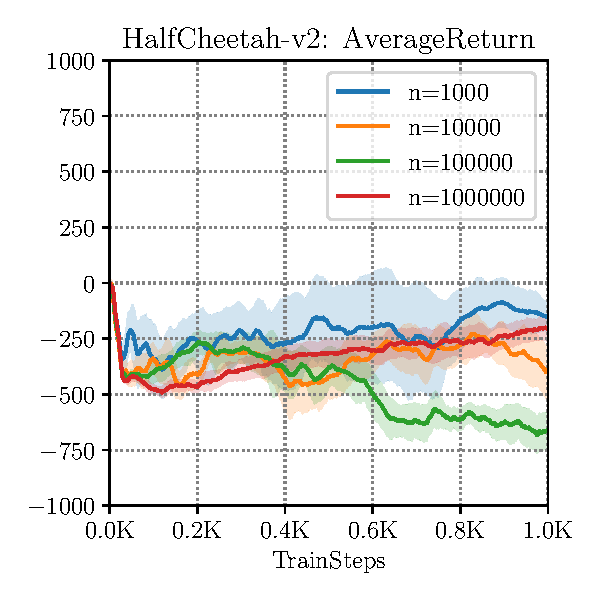
\includegraphics[width=0.45\linewidth]{chapters/bear/images/cheetah_divergence.pdf}
    ~
    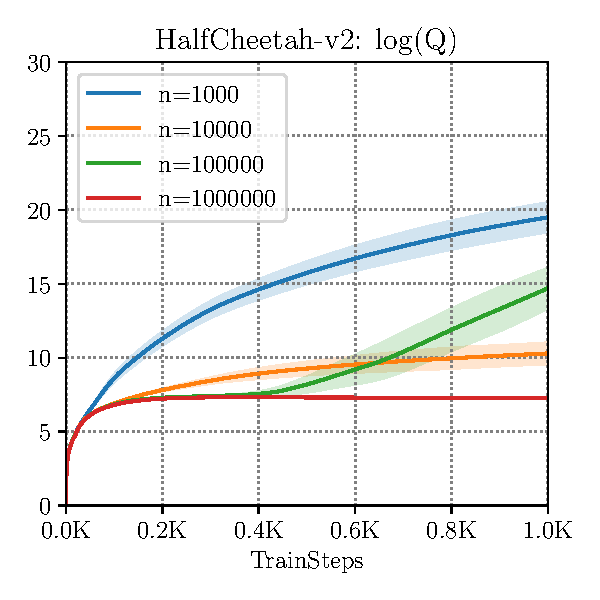
\includegraphics[width=0.45\linewidth]{chapters/bear/images/cheetah_divergence_q_val.pdf}
  \end{center}
 \vspace{-10pt}
 %%SL.5.22: Very important: the y-axes are not labeled right now, and it took me a while to figure out which plot was showing what. What is log(Q)? I guess you're trying to show that the right plot has Bellman error (?), while the left has performance? A couple more things: (1) always put space before ( (you often omit this space) (2) consider a caption like this (once the figures are labeled more clearly): Off-policy learning with SAC on HalfCheetah-v2 for different dataset sizes ($n$). The performance (left) does not correlate with $n$, while the Q-values (right) diverge or saturate at values far from the actual return.
  \caption{ \footnotesize Performance of SAC on HalfCheetah-v2 (return (left) and $\log$ Q-values (right)) with off-policy expert data w.r.t. number of training samples ($n$). Note the large discrepancy between returns (which are negative) and $\log$ Q-values (which have large positive values), which is not solved with additional samples.} 
 \vspace{-15pt}
 \label{fig:divergence}
\end{figure}
Building upon the discoveries presented in Chapter~\ref{chapter:diagnosing}, we have observed that Q-learning methods frequently struggle to learn from static, off-policy data, particularly in high-dimensional tasks. This difficulty is evident in Figure \ref{fig:divergence}. As outlined in the discussion of Chapter~\ref{chapter:diagnosing}, the primary cause of this instability lies in the challenges of handling distributional shift and statistical error. However, a crucial question remains: which factor plays a more significant role in this example? Furthermore, what mechanism underlies the emergence of this instability?

First of all, note that increasing the size of the static dataset does not rectify the problem (compare $n=1M$ vs $n=1000$), suggesting the issue in this setting is largely due to distributional shift. We can understand the source of this instability by examining the form of the Bellman backup. Although minimizing the mean squared Bellman error corresponds to a supervised regression problem, the targets for this regression are themselves derived from the current Q-function estimate. The targets are calculated by maximizing the learned $Q$-values with respect to the action at the next state. However, the $Q$-function estimator is only reliable on inputs from the same distribution as its training set. As a result, na\"{i}vely maximizing the value may evaluate the $\hat{Q}$ estimator on actions that lie far outside of the training distribution, resulting in pathological values that incur large error. We refer to these actions as out-of-distribution (OOD) actions. 

Formally, let $\valerr_k(\bs, \mathbf{a}) = |Q_k(\bs, \mathbf{a}) - Q^*(\bs, \mathbf{a})|$ denote the total error at iteration $k$ of Q-learning, and let $\projerr_k(\bs, \mathbf{a}) = |Q_k(\bs, \mathbf{a}) - \mathcal{B} Q_{k-1}(\bs, \mathbf{a})|$ denote the current Bellman error. Then, we have \mbox{$\valerr_k(\bs, \mathbf{a}) \le \projerr_k(\bs, \mathbf{a}) + \gamma \max_{\mathbf{a}'} \expec_{\bs'}[\valerr_{k-1}(\bs', \mathbf{a}')]$}. In other words, errors from $(\bs', \mathbf{a}')$ are discounted, then accumulated with new errors $\projerr_k(\bs, \mathbf{a})$ from the current iteration. We expect $\projerr_k(\bs, \mathbf{a})$ to be high on OOD states and actions, as errors at these state-actions are never directly minimized while training.

To mitigate bootstrapping error, we can restrict the policy to ensure that it output actions that lie in the support of the training distribution. This is distinct from previous work~\citep{jaques2019way} which implicitly constrains the \emph{distribution} of the learned policy to be close to the behavior policy, similarly to behavioral cloning~\cite{Schaal99isimitation}.
While this is sufficient to ensure that actions lie in the training set with high probability, it is overly restrictive. For example, if the behavior policy is close to uniform, the learned policy will behave randomly, resulting in poor performance, even when the data is sufficient to learn a strong policy (see Figure~\ref{fig:gridworld}
for an illustration). {Formally, this means that a learned policy $\pi(\mathbf{a}| \bs)$ has positive density\textit{ only where} the density of the behaviour policy $\beta(\mathbf{a}|s)$ is more than a threshold (i.e., $\forall \mathbf{a}, \beta(\mathbf{a}|\bs) \leq \varepsilon \implies \pi(\mathbf{a}|\bs) = 0$), instead of a closeness constraint on the value of the density $\pi(\mathbf{a}|\bs)$ and $\beta(\mathbf{a}|\bs)$.}
Our analysis instead reveals a tradeoff between staying within the data distribution and finding a suboptimal solution when the constraint is too restrictive. Our analysis motivates us to restrict the support of the learned policy, but not the probabilities of the actions lying within the support. This avoids evaluating the Q-function estimator on OOD actions, but remains flexible in order to find a performant policy. Our proposed algorithm leverages this insight. 

\vspace{-0.2cm}
\section{Formal Analysis and Distribution-Constrained Backups}
\label{sec:dist_constrained}
\vspace{-0.2cm}
In this section, we define and analyze a backup operator that restricts the set of policies used in the maximization of the Q-function, and we derive performance bounds which depend on the restricted set. This provides motivation for constraining policy support to the data distribution, allowing us to address the issue discussed above. We begin with the definition of a distribution-constrained operator:

\begin{tcolorbox}[colback=blue!6!white,colframe=black,boxsep=0pt,top=3pt,bottom=5pt]
\begin{definition}[Distribution-constrained operators]
Given a set of policies $\Pi$, the distribution-constrained backup operator is defined as:
%\[ \TPi Q(s, a) \coloneqq \expec \big[ R(s, a) + \gamma \expec_{\trans(s' | s, a)}\left[\max_{\pi \in \Pi} \expec_{\pi}[Q(s', a')] \right] \big] \]
\begin{align*}
\TPi Q(\mathbf{s}, \mathbf{a}) \defeq \expec \big[ R(\bs, \mathbf{a}) + \gamma \max_{\pi \in \Pi} \expec_{\trans(\bs' | \bs, \mathbf{a})}\left[V(\bs') \right] \big]
\ \ \ \ \ \ \ \ \ \ \ \ 
V(\bs) \defeq \max_{\pi \in \Pi} \expec_{\pi}[Q(\mathbf{s}, \mathbf{a})]\ \ .
\end{align*}
\end{definition}
\end{tcolorbox}
This backup operator satisfies properties of the standard Bellman backup, such as convergence to a fixed point, as discussed in Appendix~\ref{app:constrained_backup}. To analyze the (sub)optimality of performing this backup under approximation error, we first quantify two sources of error. The first is a \emph{suboptimality bias}. The optimal policy may lie outside the policy constraint set, and thus a suboptimal solution will be found. The second arises from distribution shift between the training distribution and the policies used for backups. This formalizes the notion of OOD actions. %and states.
To capture suboptimality in the final solution, we define a \emph{suboptimality constant}, which measures how far $\pi^*$ is from $\Pi$. 

\begin{definition}[Suboptimality constant]
The suboptimality constant is defined as:
\[ \alpha(\Pi) = \max_{\bs, \mathbf{a}} |\TPi Q^*(\bs, \mathbf{a}) - \backup Q^*(\bs, \mathbf{a})|. \]
\end{definition}
\vspace{-10pt}
Next, we define a concentrability coefficient~\citep{munos2005erroravi}, which quantifies how far the visitation distribution generated by policies from $\Pi$ is  from the training data distribution. This constant captures the degree to which states and actions are out of distribution.
\begin{tcolorbox}[colback=blue!6!white,colframe=black,boxsep=0pt,top=3pt,bottom=5pt]
\begin{assumption}[Concentrability]
Let $\rhoinit$ denote the initial state distribution, and $\mu(\bs, \mathbf{a})$ denote the distribution of the training data over $\mathcal{S} \times \mathcal{A}$, with marginal $\mu(\bs)$ over $\mathcal{S}$. Suppose there exist coefficients $c(k)$ such that for any $\pi_1, ... \pi_k \in \Pi$ and $s \in \mathcal{S}$:
\[
\rhoinit P^{\pi_1}P^{\pi_2}...P^{\pi_k}(s) \le c(k) \mu(\bs),
\]
where $P^{\pi_i}$ is the transition operator on states induced by $\pi_i$.
Then, define the concentrability coefficient $C(\Pi)$ as
\[
C(\Pi) \defeq (1-\gamma)^2\sum_{k=1}^\infty k\gamma^{k-1}c(k).
\] \label{assumption:conc} \end{assumption} 
\end{tcolorbox}
% \vspace{-10pt}
To provide some intuition for $C(\Pi)$, if $\mu$ was generated by a single policy $\pi$, and $\Pi = \{\pi\}$ was a singleton set, then we would have $C(\Pi)=1$, which is the smallest possible value. However, if $\Pi$ contained policies far from $\pi$, the value could be large, potentially infinite if the support of $\Pi$ is not contained in $\pi$. Now, we bound the performance of approximate distribution-constrained Q-iteration:

\begin{tcolorbox}[colback=blue!6!white,colframe=black,boxsep=0pt,top=3pt,bottom=5pt]
\begin{theorem}
\label{thm:avi_bound}
Suppose we run approximate distribution-constrained value iteration with a set constrained backup $\TPi$. Assume that $\delta(\bs,\mathbf{a}) \ge \max_k |Q_k(\bs, \mathbf{a}) - \TPi Q_{k-1}(\bs, \mathbf{a})|$ bounds the Bellman error. Then,
\[\lim_{k \to \infty} \expec_{\rhoinit}[|V^{\pi_k}(\bs) - V^*(\bs)|] \le
\frac{\gamma}{(1-\gamma)^2}\left[ C(\Pi)\expec_\mu[\max_{\pi \in \Pi} \expec_{\pi}[\projerr(\bs, \mathbf{a})]] + \frac{1-\gamma}{\gamma}\alpha(\Pi) \right]
\]
\end{theorem}
\end{tcolorbox}
\begin{proof} See Appendix~\ref{app:error_prop}, Theorem~\ref{thm:avi_bound_proof} \end{proof}
This bound formalizes the tradeoff between keeping policies chosen during backups close to the data (captured by $C(\Pi)$) and keeping the set $\Pi$ large enough to capture well-performing policies (captured by $\alpha(\Pi)$). When we expand the set of policies $\Pi$, we are increasing $C(\Pi)$ but decreasing $\alpha(\Pi)$. An example of this tradeoff, and how a careful choice of $\Pi$ can yield superior results, is given in a tabular gridworld example in Fig.~\ref{fig:gridworld}, where we visualize errors accumulated during distribution-constrained Q-iteration for different choices of $\Pi$. 

Finally, we motivate the use of support sets to construct $\Pi$. We are interested in the case where $\Pi_\epsilon = \{ \pi ~|~ \pi( \mathbf{a} | \bs) = 0 \text{ whenever } \beta( \mathbf{a} | \bs) < \epsilon \}$, where $\beta$ is the behavior policy (i.e., $\Pi$ is the set of policies that have support in the probable regions of the behavior policy). Defining $\Pi_\epsilon$ in this way allows us to bound the concentrability coefficient:

\begin{tcolorbox}[colback=blue!6!white,colframe=black,boxsep=0pt,top=3pt,bottom=5pt]
\begin{theorem}
\label{thm:conc_coeff_bound}
% Assume the data distribution $\mu$ is generated by a policy $\beta$, such that $\mu(s,a) = d_\beta(s,a)$. Let $\mu_\beta(s)$ be the state-visitation marginal for $\beta$. Let us define $\Pi_\epsilon = \{ \pi ~|~ \pi( a | s) = 0 \text{ whenever } \beta( a | s) < \epsilon \}$. Let $\mu_{\Pi}(s)$ be the maximum discounted visitation marginal of a state generated by some sequence of policies $\{\pi_i\}_{i} \in \Pi$ and let $f(\epsilon) \defeq \min_{s \in \mathcal{S}, \mu_\Pi(s) > 0} [\mu(s)]$. Then, Assumption~\ref{assumption:conc} is satisfied for a $C(\Pieps)$ that is bounded as:
% \[
% C(\Pi_\epsilon) \leq C(\beta) \cdot \Big(1 + \frac{\gamma}{(1 - \gamma) f(\epsilon)} (1 - \epsilon)\Big)
% \]
Assume the data distribution $\mu$ is generated by a behavior policy $\beta$. %, such that $\mu(s,a) = d_\beta(s,a)$. 
Let $\mu(\bs)$ be the marginal state distribution under the data distribution. Define $\Pieps = \{ \pi ~|~ \pi( \mathbf{a} | \bs) = 0 \text{ whenever } \beta( \mathbf{a} | \bs) < \epsilon \}$ and let $\mu_\Pieps$ be the highest discounted marginal state distribution starting from the initial state distribution $\rho$ and following policies $\pi \in \Pieps$ at each time step thereafter. Then, there exists a concentrability coefficient $C(\Pieps)$ which is bounded:
\[
C(\Pi_\epsilon) \leq C(\beta) \cdot \Big(1 + \frac{\gamma}{(1 - \gamma) f(\epsilon)} (1 - \epsilon)\Big)
\]
where $f(\epsilon) \defeq \min_{\bs \in \mathcal{S}, \mu_\Pieps(\bs) > 0} [\mu(\bs)] > 0$.
\end{theorem}
\end{tcolorbox}
% \vspace{-10pt}
\begin{proof} See Appendix~\ref{app:error_prop}, Theorem~\ref{thm:conc_coeff_proof} \end{proof}
% \vspace{-10pt}
Qualitatively, $f(\epsilon)$ is the minimum discounted visitation marginal of a state under the behaviour policy if only actions which are more than $\epsilon$ likely are executed in the environment. Thus, using support sets gives us a single lever, $\epsilon$, which simultaneously trades off the value of $C(\Pi)$ and $\alpha(\Pi)$. Not only can we provide theoretical guarantees, we will see in our experiments (Sec.~\ref{sec:experiments}) that constructing $\Pi$ in this way provides a simple and effective method for implementing distribution-constrained algorithms. 

Intuitively, this means we can prevent an increase in overall error in the Q-estimate by selecting policies supported on the support of the training action distribution, which would ensure roughly bounded projection error $\delta_k(\mathbf{s}, \mathbf{a})$ while reducing the suboptimality bias, potentially by a large amount. Bounded error $\delta_k(\bs, \mathbf{a})$ on the support set of the training distribution is a reasonable assumption when using highly expressive function approximators, such as deep networks, especially if we are willing to reweight the transition set~\cite{Schaul2015,fu2019diagnosing}. We further elaborate on this point in Appendix~\ref{app:bearql-more}.

\begin{figure}
    \centering
    \vspace{-0.1in}
    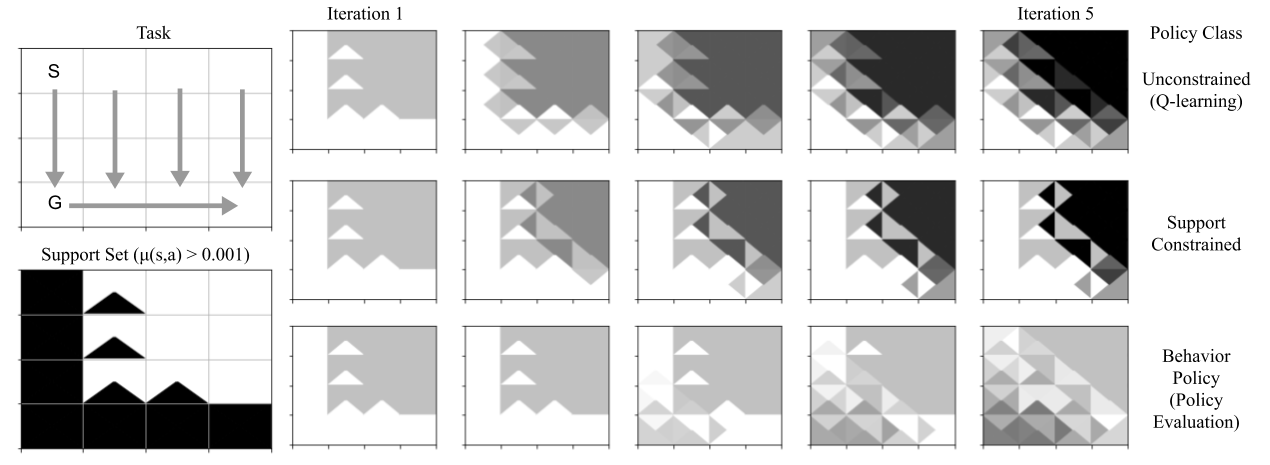
\includegraphics[width=0.9\textwidth]{chapters/bear/images/gridworld}
    \caption{ \footnotesize Visualized error propagation in Q-learning for various choices of the constraint set $\Pi$:
    unconstrained (top row) distribution-constrained (middle),
    and constrained to the behavior policy (policy-evaluation, bottom). Triangles represent Q-values for actions that move in different directions. The task (left) is to reach the bottom-left corner (G) from the top-left (S), but the behaviour policy (visualized as arrows in the task image, support state-action pairs are shown in black on the support set image) travels to the bottom-right with a small amount of $\epsilon$-greedy exploration. Dark values indicate high error, and light values indicate low error. Standard backups propagate large errors from the low-support regions into the high-support regions, leading to high error. Policy evaluation reduces error propagation from low-support regions, but introduces significant suboptimality bias, as the data policy is not optimal. A carefully chosen distribution-constrained backup strikes a balance between these two extremes, by confining error propagation in the low-support region while introducing minimal suboptimality bias.}
    \label{fig:gridworld}
    \vspace{-0.1in}
\end{figure}

% \subsection{Choosing Backup Policies for OOD Action Error Reduction}
% \label{sec:choosing_policies}
% Argument in Sec.~\ref{sec:tradeoff} tells us that, with a careful selection of the policy under which the target value is computed, the overall error of value estimates from the optimal value function $\|V^* - V_k\|$ can be reduced. How should we search for a policy that minimizes the overall error? Our choice is to backup from policies which maintain high-support over the action set of the data.
% %%SL.5.22: I think it's not obvious to readers that "policy for the backup" means the distribution over the actions under which the target value is calculated. -- addressed

% To justify this choice,
% %%SL.5.22: What choice? -- choice of backing up from any policy that maintains high support over data.
% we note that the error analysis relies on being able to quantify $\delta_k(s, a)$ (the per-state-action bellman error) for OOD actions. Outside of the support of the data distribution, it is hard to provide guarantees on $\delta_k$. However, when $a$ lies inside the support of the training distribution for a given state $s$, high-capacity function approximators trained with supervised learning are expected to produce a bounded error, given enough samples.
% %Even if they don't produce bounded error on such in-support inputs, techniques such as Prioritized Replay~\cite{Schaul2016PrioritizedER} can be employed to ensure bounded error on all in-support inputs. 
% %Furthermore, often the quantity of interest is the Bellman error weighted by the inverse density of the behaviour policy~\cite{antos07fitted}, which depends only on the support of the behaviour policy and this error metric is the equal for two policies provided they share the same support.
% Therefore, backing up from all actions that have non-negligible support under the training distribution is sufficient (but not necessary) to prevent error accumulation. Hence, we restrict the set $\Pi$
% %%SL.5.22: Did we define \Pi before? since we cut the set backup operator stuff, now this is much harder to follow. Maybe we can bring it back (but call it something else)?
% of policies used for distribution-constrained backups to the set of policies that are supported on the probable regions of the behaviour policy. That is, $\Pi = \{ \pi | \pi( a | s) = 0 \text{ whenever } \beta( a | s) < \epsilon \}$, where $\beta$ is the behavior policy (i.e., the set of policies that have support in the probable regions of the behavior policy). This means that we are allowed to backup from any action distribution supported over the support of the behaviour policy. Previous work~\cite{fujimoto2018off} restricts the choice of actions to be a distribution close to the behaviour policy. 

%%SL.5.22: I don't really understand what the above paragraph is saying. Read literally, it seems to say "prior work does something similar, and in the worst case we are equally bad." That's not very satisfying. Maybe just delete this paragraph, or rephrase if that's not what you meant?
%Now, explain why this does a good job of balancing the terms. Next, we explain how this bound motivates the use of set-constrained backups to reduce accumulation of bootstrapping error. \TODO{explanation about $\delta1$ goes here} -- addressed -- removed this paragraph


% we need to determine how to formulate the appropriate constraint and how to implement so as to back up only values of policies in $\Pi$.
% %%SL.5.20: Rephrase. In order to develop a practical algorithm based on the set-constrained backup, we need to determine how to formulate the appropriate constraint and how to implement so as to back up only values of policies in $\Pi$.
% Intuitively, we would like $\Pi(s)$ for a particular state $s$ to contain only those policies that permit actions within the support of the dataset distribution. Instead of inferring $\Pi$, we use a notion of divergence between the uniform distribution over the support-set of the current policy and the current policy for optimization.  

% %%SL.5.20: Rephrase. Intuitively, we would like $\Pi(s)$ for a particular state $s$ to contain only those policies that permit actions withi
% In order confidence support set perform the $\max$ on the high-over actions from only these policies, we need to define a tractable objective. Instead of inferring the set of policies $\Pi$ we rather resort to specifying a notion of divergence between the set $\mathcal{A}_\varepsilon^\dataset$ and the current policy, $\operatorname{Divergence}(\mathcal{A}^{\mathcal{D}}_{\varepsilon}(s), \pi)$ thereby fitting the problem of inferring $\Pi$ in an optimization setup.
% %%SL.5.20: I don't really understand the above sentence. Try rewriting it to be clearer?
% Next, we move on to presenting our method, which we call \emph{bootstrap error accumulation reduction} (BEAR).

\vspace{-0.2cm}
\section{Bootstrapping Error Accumulation Reduction (BEAR)}
\label{sec:bear}
\vspace{-0.2cm}

% \vspace{-0.1in}
We now propose a practical actor-critic algorithm (built on the framework of TD3~\cite{fujimoto18addressing} or SAC~\cite{haarnoja2018sac}) that uses distribution-constrained backups to reduce accumulation of bootstrapping error. The key insight is that we can search for a policy with the same support as the training distribution, while preventing accidental error accumulation.
Our algorithm has two main components. Analogous to BCQ~\citep{fujimoto18addressing}, we use $K$ Q-functions and use the minimum Q-value for policy improvement, and design a constraint which will be used for searching over the set of policies $\Pieps$, which share the same support as the behavior policy. Both of these components will appear as modifications of the policy improvement step in actor-critic style algorithms. We also note that policy improvement can be performed with the mean of the K Q-functions, and we found that this scheme works as good in our experiments. 

% n components. Analogous to BBCQ~\citep{fujimoto2018off}, we use two Q-functions and linearly combine their predictions the Q-function for policy improvement, and design a constraint which will be used for searching over the set of policies $\Pieps$, which share the same support as the behaviour policy. Both of these components will appear as modifications of the policy improvement step in actor-critic style algorithms.

We denote the set of Q-functions as: $\hat{Q}_1, \cdots, \hat{Q}_K$.
% compute a conservative estimate of the Q-values: $\frac{1}{K} \sum_{i=1}^K \hat{Q}_i (s, a) - \lambda \sqrt{\operatorname{var}_k \hat{Q}_k(s, a)}$, where $\lambda \in \mathbb{R}^+$ is a hyperparameter. %We use this value as a conservative estimate of the Q-function. This can be derived using Cantelli's inequality. 
Then, the policy is updated to maximize the conservative estimate of the Q-values within $\Pieps$: 
% \vspace{-10pt}
$$ \pi_\phi(\bs) := \max_{\pi \in \Pieps} \expec_{a \sim \pi(\cdot|\bs)} \left[\min_{j=1,..,K} \hat{Q}_j(\bs, \mathbf{a})\right] $$
% \lambda \sqrt{ \operatorname{var_k}\expec_{a \sim \pi(\cdot |s) }[\hat{Q}_k(s, a)]}.$$
% \vspace{-5pt}
% Let $\mathcal{F}_t$ be the sigma-algebra generated by the training procedure until iteration $t$, and let $\operatorname{var}_{t} \hat{Q}(s,a) := \mathbb{E}[(\hat{Q}_t(s, a) - \mathbb{E}[(\hat{Q}_t(s, a) | \mathcal{F}_t))^2|\mathcal{F}_t]$
%%SL.5.20: use mbox. And for clarity, it might be good to indicate what the expectation is over (and use [ instead of ( for E so that parens don't get cluttered). Also, what is up with this (s,a) hanging out at the end? do you mean to put (s,a) inside (after \hat{Q})?
% denote the variance of the Q-function $\hat{Q}_t$, at time $t$ during training. Then, for each state-action pair $(s, a)$, 
% ${Pr (\hat{Q}_t \geq \mathbb{E}(\hat{Q}_t|\mathcal{F}_t) + \sqrt{\frac{(1 - \delta) \operatorname{var}_{t} \hat{Q}_t }{\delta}})  \leq \delta}$
%%SL.5.20: can you state in words what this means for the purpose of this section? also, rhetoric-wise, amybe better state as a theorem (it's kind of obvious, but still) and then after say that this is easy to show via Cantelli's inequality or something?

%%SL.5.20: It's not clear what the concentration bound is actually used for.

 %In the above concentration bound, $\mathbb{E}(\hat{Q}_t|\mathcal{F}_t)$ refers to the true Q-value, which can be obtained given no stochasticity in the procedure.


%%SL.5.20: The logical thread here is broken. What are you doing with set divergence? State the issue first, then th e resolution, else it's hard for the reader to follow.
In practice, the behavior policy $\beta$ is unknown, so we need an approximate way to constrain $\pi$ to $\Pi$. We define a differentiable constraint that approximately constrains $\pi$ to $\Pi$, and then approximately solve the constrained optimization problem via dual gradient descent.  We use the sampled version of maximum mean discrepancy (MMD)~\cite{gretton2012kernel}
%%SL.5.22: Alg names are not capitalized unless they contain proper nouns, put a space after the words and before open paren (I fixed it above, but this issue happens often, please take this comment into account) -- Thanks for pointing this out!
between the unknown behavior policy $\beta$ and the actor $\pi$ because it can be estimated based solely on samples from the distributions. Given samples $x_1, \cdots, x_n \sim P$ and $y_1, \cdots, y_m \sim Q$, the sampled MMD between $P$ and $Q$ is given by:\\
$$\operatorname{MMD}^2(\{x_1, \cdots, x_n\}, \{y_1, \cdots, y_m\}) = \frac{1}{n^2} \sum_{i, i'} k(x_i, x_{i'}) - \frac{2}{nm} \sum_{i, j} k(x_i, y_j) + \frac{1}{m^2} \sum_{j, j'} k(y_j, y_{j'}).
$$
Here, $k(\cdot, \cdot)$ is any universal kernel. In our experiments, we find both Laplacian and Gaussian kernels work well.
%As the $\operatorname{MMD}$ distance does not depend on the density function of either distribution, minimizing it using samples is a reasonable proxy for enforcing that $Q$ lies inside the support of $P$. This is because, 
The expression for MMD does not involve the density of either distribution and it can be optimized directly through samples. Empirically we find that, in the low-intermediate sample regime, the sampled MMD between $P$ and $Q$ is similar to the MMD between a uniform distribution over $P$'s support and $Q$, which makes MMD roughly suited for constraining distributions to a given support set. (See Appendix~\ref{app:mmd} for numerical simulations justifying this approach).

% and hence, we parameterize the set $\mathcal{A}^{\mathcal{D}}_{\varepsilon}(s)$ as a distribution $\pi_{set}(a|s)$ such that $\mathcal{A}(s) := \mathcal{A}^{\pi_{set}}_{\varepsilon}(s) := \{a \in \mathcal{A} | \pi_{set}(a|s) \geq \varepsilon \}$, in other words, $\mathcal{A}(s)$ is the high-confidence support set of the distribution $\pi_{set}$, and we train for a parametric $\pi_{set}$.
%%SL.5.20: I don't actually understand at this point what you are doing. Are you optimizing a neural net that denotes \pi_set? or something else?

% \paragraph{Deriving the update:} Let $\hat{Q}_k$ be the Q-function at the k-th step of the algorithm. Actor-critic Q-learning algorithms maintain a parameterized policy, $\pi_k$ that is updated towards the maximizing the Q-function.
% %-- $\pi_{k+1}(s) := \max_{\pi \in \Delta_{|S|}} E_{a \sim \pi(\cdot|s)} [\hat{Q}_{k}(s, a)]$. 
% In order to reduce the number of moving parts, we let the actor in this case serve both its regular function of maximizing the Q-function while also constraining the action distribution close to $\mathcal{A}^\dataset_\varepsilon$, which is the the task of $\pi_{set}$. We use the bound derived on Q-values to update the policy in the direction of maximizing a conservative estimate of the true Q-value -- $$ \pi_{k+1}(s) := \max_{\pi \in \Delta_{|S|}} E_{a \sim \pi(\cdot|s)} [\hat{Q}_{k}(s, a)] - \lambda \sqrt{ \operatorname{var_k}E_{a \sim \pi(\cdot |s) }[\hat{Q}_k(s, a)]}$$
% %TODO{may want to mention that this amounts to subtracting a constant times the std, which sounds reasonable}
% We still need to account for the problem of specifying support divergence. In order to enforce this constraint, we use a measure of support matching between the training distribution $\Pi$ and the policy $\pi(\cdot|s)$, which we choose to be a sampled version of the Maximum Mean Discrepancy(MMD) Distance between $\Pi$ and the actor $\pi$. Sampled MMD distance between two probability distributions $P$ and $Q$ is given by, $\operatorname{MMD}(P, Q)$, where $x_1, \cdots, x_n \sim P$ and $y_1, \cdots, y_m \sim Q$ is given by:\\
% $$\operatorname{MMD}^2(\{x_1, \cdots, x_n\}, \{y_1, \cdots, y_m\}) = \frac{1}{n^2} \sum_{i, i'} k(x_i, x_{i'}) - \frac{2}{nm} \sum_{i, j} k(x_i, y_j) + \frac{1}{m^2} \sum_{j, j'} k(y_j, y_{j'})
% $$
% When the number of samples $n$ is an intermediate number (4-10), the above sampled objective can also be approximately considered as a distance between a uniform distribution over the high confidence support set of the distribution $P$ and the distribution $Q$ -- therefore, if trained perfectly, $Q$ should have the same support as $P$. That is, $\operatorname{MMD}(P, Q)$ is a reasonable proxy for $\operatorname{MMD}(\mathcal{U}(\mathcal{A}_{\varepsilon}(P)), Q)$. 
% %\TODO{what does it mean MMD between a set and distribution}
% The expression for $\operatorname{MMD}$ does not use the density function of either distribution, thereby making it suited as an approximate way of support matching.

Putting together, the optimization problem in the policy improvement step is
% \vspace{-5pt}
\begin{multline}
    \label{eqn:policy_update}
   \pi_\phi := \max_{\pi \in \Delta_{|S|}} \expec_{\bs \sim \mathcal{D}} \expec_{\mathbf{a} \sim \pi(\cdot|\bs)} \left[\min_{j=1,..,K} \hat{Q}_j(\bs, \mathbf{a})\right] 
%   - \lambda \sqrt{ \operatorname{var_k}\expec_{a \sim \pi(\cdot |s) }[\hat{Q}_k(s, a)]}\\
   \text{~~s.t.~~} \mathbb{E}_{\bs \sim \mathcal{D}} [\operatorname{MMD}(\mathcal{D}(\bs), \pi(\cdot|\bs))] \leq \varepsilon \quad
\end{multline}
where $\varepsilon$ is an approximately chosen threshold. We choose a threshold of $\varepsilon=0.05$ in our experiments. The algorithm is summarized in Algorithm~\ref{algo:bear_ql}. 
% Step 5 of the algorithm performs a stochastic version of the distribution-constrained backup, where Dirac-delta policies $\delta_{a_i}, \cdots, \delta_{a_p},(~\forall~i, \delta_{a_i} \in \Pi)$ are sampled, an expectation of the target Q-value under these Dirac-delta policies is computed and then the maximum value across these policies is backed up as defined by the backup operator. We provide more explanation in Appendix \ref{app:bearql-more}.

\textbf{How does BEAR connect with distribution-constrained backups described in Section 4.1?} Step 5 of the algorithm restricts $\pi_\phi$ to lie in the support of $\beta$. This insight is formally justified in Theorems 4.1 \& 4.2 ($C(\Pi_\varepsilon)$ is bounded). Computing distribution-constrained backup exactly by maximizing over $\pi \in \Pi_\varepsilon$ is intractable in practice. As an approximation, we sample Dirac policies in the support of $\beta$ (Alg 1, Line 5) and perform empirical maximization to compute the backup. As the maximization is performed over a \textit{narrower} set of Dirac policies ($\{ \delta_{\mathbf{a}_i} \} \subseteq \Pi_\varepsilon$), the bound in the above Theorem still holds. Empirically, we show in Section~\ref{sec:experiments} that this approximation is sufficient to outperform previous methods. This connection is briefly discussed in Appendix~\ref{app:bear_dist_constrained}.
% $\operatorname{var}(\hat{Q}_k(s, a)) \approx \frac{1}{M} \sum_{i=1}^{M} (\hat{Q}_{\theta_i, k}(s, a) - \bar{Q}_{\theta, k}(s, a))^2$, where $\bar{Q}_{\theta, k}(s, a) = \frac{1}{M} \sum_{i=1}^{M} \hat{Q}_{\theta_i, k}(s, a)$ is the sample mean of the ensemble. 

%AK.05.15: Note to Sergey: this is the actor-critic version, optional depends on results.
% Another variant of the above approach can be where this single policy improvement step can be decomposed into two decoupled steps -- (1) Learning a policy $\pi_{set}$, whose high-confidence set defines the support set $\mathcal{A}_{\varepsilon}(s)$ at a state $s$, by minimizing the sampling error in $\hat{Q}_k$ and accounting for the deviation from the dataset, and then, (2) Learning to maximize the expected Q-function $\hat{Q}_k$ on this set $\mathcal{A}_{\varepsilon}(s)$, in practice obtained by sampling from $\pi_{set}$. In practice, we found using Equation~\ref{eqn:policy_update} working better than the latter approach and hence, we stick to this formulation for our experiments. The overall algorithm is summarized in Algorithm~\ref{alg:q_learning}, and the actor-critic version is described in Algorithm~\ref{alg:actor_critic}.   
% \vspace{-5pt}
\begin{algorithm}[h]
\small
\caption{Q-learning variant of BEAR (BEAR)}
\label{alg:q_learning}
\begin{algorithmic}[1]
    \State Dataset $\mathcal{D}$, target network rate $\tau$, batch size $N$, sampled actions for MMD $n$, minimum $\lambda$
    \State Initialize Q-ensemble $\{Q_{\theta_i} \}_{i=1}^{K}$, actor $\pi_{\phi}$, multiplier $\alpha$, target networks $\{ Q_{\theta'_i} \}_{i=1}^K$, and a target actor $\pi_{\phi'}$, with $\phi' \leftarrow \phi, \theta'_i \leftarrow \theta_i$
    \ForAll{$t$ in \{1, \dots, N\}}
        \State Sample mini-batch of transitions $(\bs, \mathbf{a}, r, \bs') \sim \mathcal{D}$\\
        \textbf{Q-update:}
            \State Sample $p$ action samples, $\{\mathbf{a}_i \sim \pi_{\phi'}(\cdot|\bs')\}_{i=1}^p$
            \State Define $y(\bs, \mathbf{a}) := \max_{\mathbf{a}_i} [ \lambda \min_{j=1,..,K} Q_{\theta'_j}(\bs', \mathbf{a}_i) + (1 - \lambda) \max_{j=1,..,K} Q_{\theta'_j}(\bs', \mathbf{a}_i)]$
            \State $\forall i, \theta_i \leftarrow \arg \min_{\theta_i} (Q_{\theta_i}(\bs, \mathbf{a}) - (r + \gamma y(\bs, \mathbf{a})))^2$\\
        \textbf{Policy-update:}
        \State Sample actions $\{ \hat{\mathbf{a}}_i \sim \pi_{\phi}(\cdot | \bs) \}_{i=1}^{m}$ and $\{ \mathbf{a}_j \sim \mathcal{D}(\bs)\}_{j=1}^{n}$. % $n$ preferably an intermediate integer(1-10)
        \State Update $\phi$, $\alpha$ by minimizing Equation~\ref{eqn:policy_update} with Lagrange multiplier $\alpha$.
        \State \textbf{Update Target Networks: } $\theta'_i \leftarrow \tau \theta_i + (1 - \tau)\theta'_i$; $\phi' \leftarrow \tau \phi + (1 -\tau) \phi'$ 
    \EndFor
\end{algorithmic}
\label{algo:bear_ql}
\end{algorithm}

In summary, the actor is updated towards maximizing the Q-function while still being constrained to remain in the valid search space defined by $\Pieps$. The Q-function uses actions sampled from the actor to then perform distribution-constrained Q-learning, over a reduced set of policies. {At test time, we sample $p$ actions from $\pi_\phi(\bs)$ and the Q-value maximizing action out of these is executed in the environment.}  %The maximization step in the actor-update empirically helps, but can be coupled with maximization in Step 5. Similar to \cite{fujimoto2018off} we use a soft-minimum to compute target values for updating Q-functions. 
Implementation and other details are present in Appendix \ref{app:bear_additional_details}.
%%SL.5.22: Remember to fill this in.

% \begin{algorithm}[H]
% \small
% \caption{BEAR Actor-Critic}
% \label{alg:actor_critic}
% \begin{algorithmic}[1]
%     \INPUT: Dataset $\mathcal{D}$, target network update rate $\tau$, mini-batch size $N$, sampled actions for MMD $n$, minimum $\lambda$, policy gradient clipping constants $\beta_1, \beta_2; \beta_1 \leq \beta_2$, MMD threshold constant $\varepsilon$
%     \STATE Initialize Q-ensemble $\{Q_{\theta_i} \}_{i=1}^{M}$, actor $\pi_{\phi}$, set-determining policy $\pi_{set}$, Lagrange multiplier $\alpha$, target networks $\{ Q_{\theta'_i} \}_{i=1}^M$, and a target actor $\pi_{\phi'}$, with $\phi' \leftarrow \phi, \theta'_i \leftarrow \theta_i$
%     \FOR{$t$ in \{1, \dots, N\}}
%         \STATE Sample mini-batch of transitions $(s, a, r, s') \sim \mathcal{D}$\\
%         \textbf{Q-update:}
%             \STATE Sample $m$ action samples, $\{a_i \sim \pi_{\phi'}(\cdot|s')\}_{i=1}^n$
%             \STATE Define $y = \frac{1}{m} \sum_{a_i} [ \lambda \min_{j=1,..,M} Q_{\theta'_j}(s', a_i) + (1 - \lambda) \max_{j=1,..,M} Q_{\theta'_j}(s', a_i)]$
%             \STATE $\forall i, \theta_i \leftarrow \arg \min_{\theta_i} (Q_{\theta_i}(s, a) - (r + \gamma y))^2$\\
%         \textbf{Set-update and Actor-update:}
%         \STATE Sample actions $A_1(s) \equiv \{ \hat{a}_i \sim \pi_{set}(\cdot | s) \}_{i=1}^{m}$ and $A_2(s) \equiv \{ a_j \sim \mathcal{D}(s)\}_{j=1}^{n}$, $n << m$
%         \STATE Update $\pi_{set}, \alpha$: $$ \pi_{set}, \alpha \leftarrow \arg \min_{\pi_{set}} \max_{\alpha \geq 0} \sqrt{\frac{(1 - \delta) \operatorname{var_k}E_{a \sim \pi_{set}(\cdot |s) }[\hat{Q}_k(s, a)]}{\delta}} + \alpha \mathbb{E}_{s \sim \mathcal{D}} ([\operatorname{MMD}(A_1, A_2)] -  \varepsilon) $$
%         \STATE Update $\phi$ using Importance Sampled Policy Gradient: 
%         $$ \pi_{\phi} \leftarrow  \max_{\pi_{\phi}} \mathbb{E}_{s \sim \mathcal{D}} \mathbb{E}_{a \sim \pi_{set}(\cdot|s)} \Big( \Big[ \frac{\pi_\phi(a|s)}{\pi_{set}(a|s)} \Big]_{\beta_1}^{\beta_2} Q(s, a) \Big)$$
%         \STATE \textbf{Update Target Networks: } $\theta'_i \leftarrow \tau \theta_i + (1 - \tau)\theta'_i$; $\phi' \leftarrow \tau \phi + (1 -\tau) \phi'$ 
%     \ENDFOR
% \end{algorithmic}
% \end{algorithm}


% Let $\bar{Q}(\cdot, \cdot)$ be the delayed target network, and $Q(\cdot, \cdot)$ be the current Q-function. Define $d_i$ be the the TD error for the $i^{th}$ datapoint.
% $$
% d_{i}(Q ; \bar{Q}, \pi)=R_{t}+\gamma \bar{Q}\left(s'_{i}, \pi_{set} \left(s'_i\right)\right)-Q\left(s_{i}, a_{i}\right)

% $$
% Further we define the empirical loss function by
% $$
% \hat{L}_{N}(Q ; \bar{Q}, \pi)=\frac{1}{N} \sum_{t=1}^{N} \frac{d_{t}^{2}(Q ; \bar{Q}, \pi_{set})}{\lambda(\mathcal{A})}
% $$
% where normalization $\lambda{\mathcal{A}}$ is introduced for mathematical convenience. Then, each policy evaluation step can be written as:  

% If we solely backup from actions present in our dataset, there is no way the algorithm can perform better than the policy that collected the data. The capacity of Q-learning and other ADP algorithms to ``stitch'' together performant sub-trajectories is lost. Hence, our method does allow the agent to backup from actions that occur outside the dataset, while still being constrained to not go farther away from the support of $\mathcal{D}$. In principle, a measure of distance from a given dataset can only be obtained using Bayesian Approaches (?). In practice, we use the variance of the ensemble as a measure to approximately quantify closeness to the support set. Our overall approach is described in the next paragraph.




% Our problem setting does not allow any interaction with the environment, and only lets us use the dataset $\mathcal{D}$. Since we see a limited subset of state-action pairs from the environment, the expected estimate of the Q-function conditioned on all training history in our case, $\mathbb{E}(\hat{Q}|\mathcal{F}_t)$, is biased. \TODO{aviral: finish this argument} 

% We train an ensemble of $N$ parametric Q-functions, $Q_{\theta_1}, \cdots, Q_{\theta_N}$ by using bootstrap masks on the data points of the dataset $\mathcal{D}$. This is done to simulate epistemic variance. To make sure that the actions chosen for backing up Q-functions are valid, we learn a set selection policy, $\pi_{set}$ -- a policy that can provide high densities to actions that don't propagate errors.   
% \section{Experimental Evaluation}
\label{sec:experiments}
In our experiments, we study how BEAR performs when learning from static offline data on a variety of continuous control benchmark tasks. We evaluate our algorithm in three settings: when the dataset $\dataset$ is generated by \textbf{(1)} a completely random behavior policy, \textbf{(2)} a partially trained, medium scoring policy, and \textbf{(3)} an optimal policy. Condition \textbf{(2)} is of particular interest, as it captures many common use-cases in practice, such as learning from imperfect demonstration data (e.g., of the sort that are commonly available for autonomous driving~\cite{DBLP:conf/iclr/GaoXLYLD18}), or reusing previously collected experience during off-policy RL. We compare our method to several prior methods: a baseline actor-critic algorithm (TD3), the BCQ  algorithm~\citep{fujimoto2018off}, which aims to address a similar problem, as discussed in Section~\ref{sec:Problem Description}, KL-control~\citep{jacques19way} (which solves a KL-penalized RL problem similarly to maximum entropy RL), a static version of DQfD~\citep{hester2018dqfd} (where a constraint to upweight Q-values of state-action pairs observed in the dataset is added as an auxiliary loss on top a regular actor-critic algorithm), and a behavior cloning (BC) baseline, which simply imitates the data distribution. This serves to measure whether each method actually performs effective RL, or simply copies the data. We report the average evaluation return over 5 seeds of the policy given by the learned algorithm, in the form of a learning curve as a function of number of gradient steps taken by the algorithm. These samples are only collected for evaluation, and are not used for training.

\subsection{Performance on Medium-Quality Data}

We first discuss the evaluation of condition with ``mediocre'' data \textbf{(2)}, as this condition resembles the settings where we expect training on offline data to be most useful. We collected one million transitions from a partially trained policy, so as to simulate imperfect demonstration data or data from a mediocre prior policy.
In this scenario, we found that BEAR consistently outperforms BCQ~\cite{fujimoto2018off} and a na\"ive off-policy RL baseline (TD3) (by large margins), as shown in Figure~\ref{fig:mediocre}. This scenario is the most relevant from an application point of view, as access to optimal data may not be feasible, and random data might have inadequate exploration to efficient learn a good policy. We also evaluate the accuracy with which the learned Q-functions predict actual policy returns. These trends are provided in Appendix~\ref{app:q_vs_mc}. 
% Note that the performance of BCQ often tracks the performance of the BC baseline, suggesting that BCQ primarily imitates the data. 
Our KL-control baseline uses automatic temperature tuning~\citep{haarnoja2018sac}. We find that KL-control usually performs similar or worse to BC, whereas DQfD tends to diverge, and often exhibits a huge variance across different runs (for example, HalfCheetah-v2 environment).  

\begin{figure}
    \centering
    \begin{subfigure}[t]{0.23\textwidth}
        \centering
        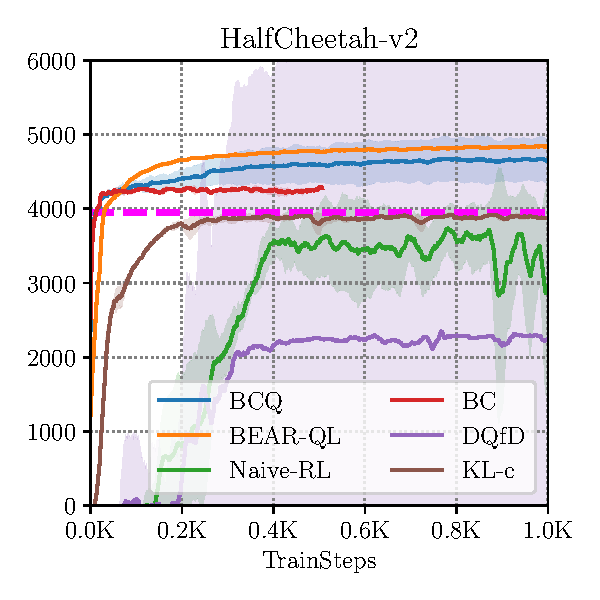
\includegraphics[width=0.99\linewidth]{chapters/bear/images/images_camera_ready/cheetah_mediocre_camera_ready.pdf}
    \end{subfigure}
    \begin{subfigure}[t]{0.23\textwidth}
        \centering
        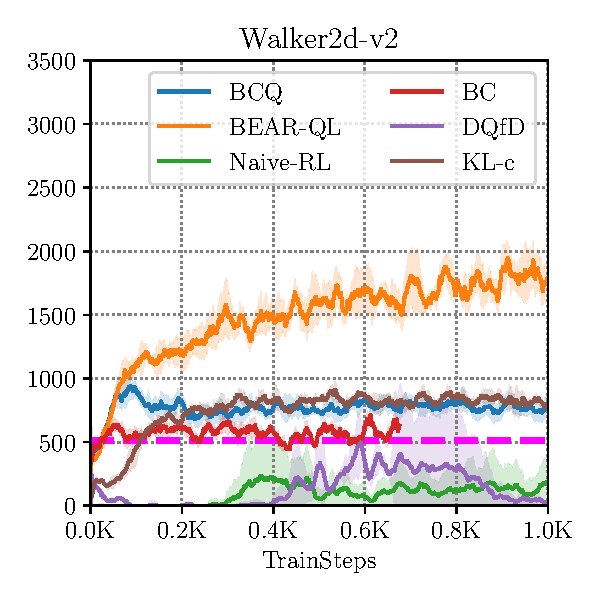
\includegraphics[width=0.99\linewidth]{chapters/bear/images/images_camera_ready/walker_mediocre_camera_ready.pdf}
        % \caption{}
    \end{subfigure}
    ~
    \begin{subfigure}[t]{0.23\textwidth}
        \centering
        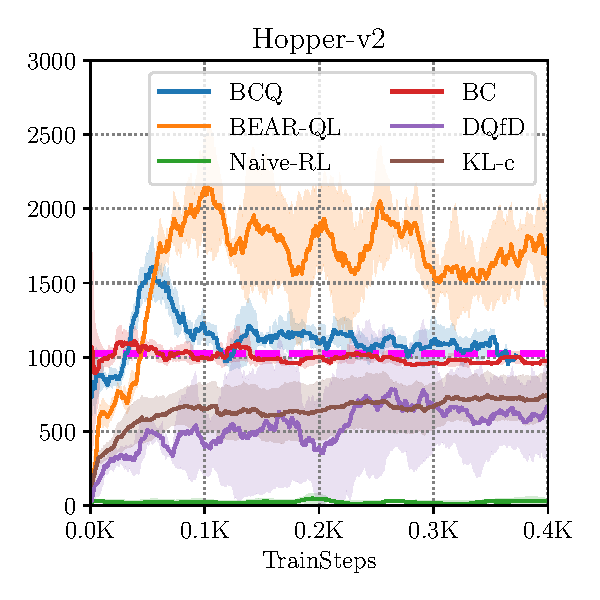
\includegraphics[width=0.99\linewidth]{chapters/bear/images/images_camera_ready/hopper_mediocre_camera_ready.pdf}
        % \caption{}
    \end{subfigure}
    ~
    \begin{subfigure}[t]{0.23\textwidth}
        \centering
        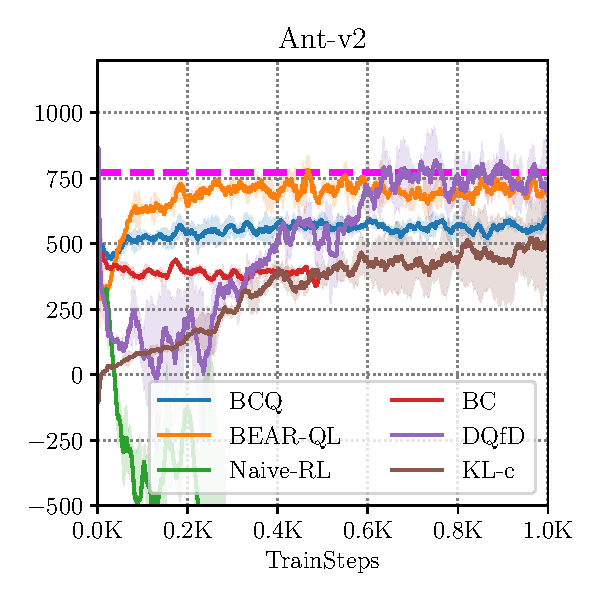
\includegraphics[width=0.99\linewidth]{chapters/bear/images/images_camera_ready/ant_mediocre_camera_ready.pdf}
        % \caption{}
    \end{subfigure}
    \caption{\label{fig:mediocre} \footnotesize Average performance of BEAR, BCQ, Na\"ive RL and BC on medium-quality data averaged over 5 seeds. BEAR outperforms both BCQ and Na\"ive RL. Average return over the training data is indicated by the magenta line. One step on the x-axis corresponds to 1000 gradient steps.}
\end{figure}

% \begin{figure*}[t!]
%     \centering
%     \vspace{-0.05in}
%     \begin{subfigure}[t]{0.23\textwidth}
%         \centering
%         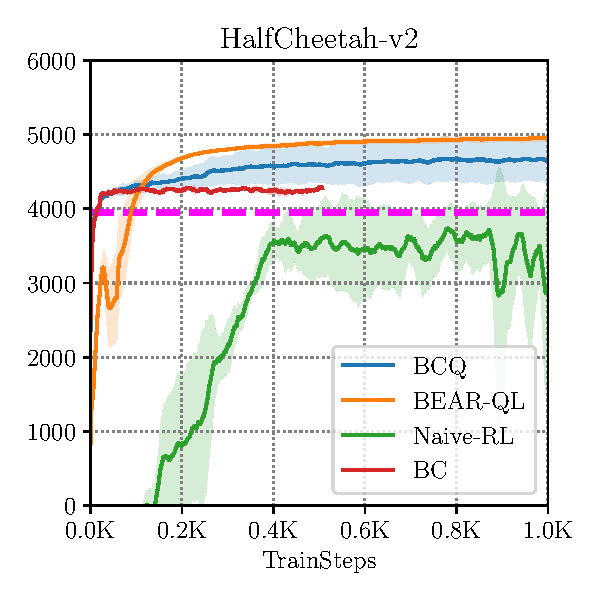
\includegraphics[width=0.99\linewidth]{chapters/bear/images/cheetah_mediocre.pdf}
%     \end{subfigure}
%     \begin{subfigure}[t]{0.23\textwidth}
%         \centering
%         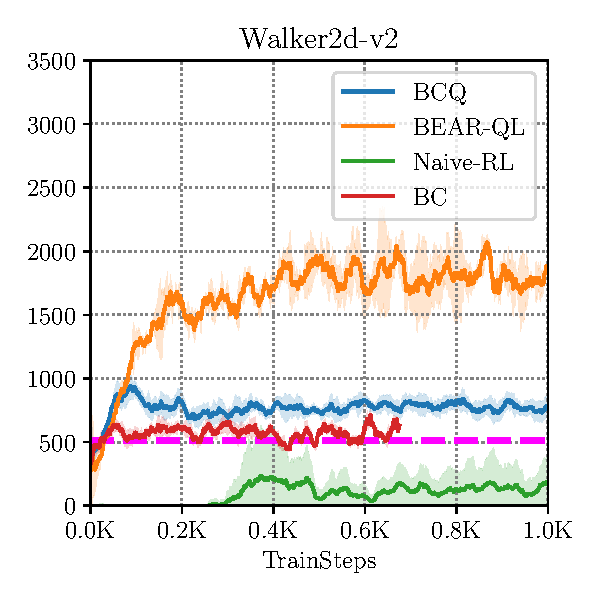
\includegraphics[width=0.99\linewidth]{chapters/bear/images/walker_mediocre_final_again.pdf}
%         % \caption{}
%     \end{subfigure}
%     ~
%     \begin{subfigure}[t]{0.23\textwidth}
%         \centering
%         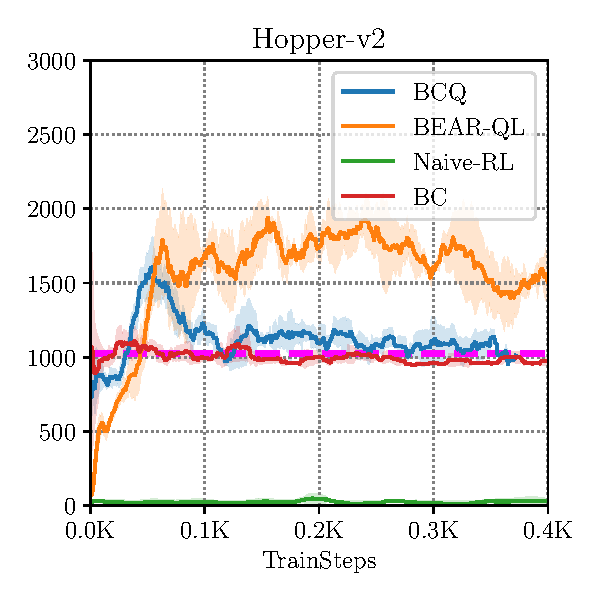
\includegraphics[width=0.99\linewidth]{chapters/bear/images/hopper_mediocre_final_new.pdf}
%         % \caption{}
%     \end{subfigure}
%     ~
%     \begin{subfigure}[t]{0.23\textwidth}
%         \centering
%         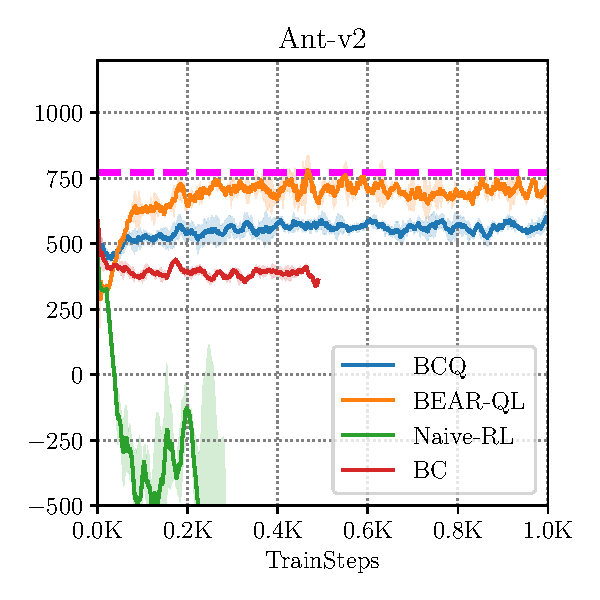
\includegraphics[width=0.99\linewidth]{chapters/bear/images/ant_mediocre_final.pdf}
%         % \caption{}
%     \end{subfigure}
%     \caption{ \footnotesize Average performance of BEAR, BCQ, Na\"ive RL and BC on medium-quality data averaged over 5 seeds. BEAR outperforms both BCQ and Na\"ive RL. Average return over the training data is indicated by the magenta line. One step on the x-axis corresponds to 1000 gradient steps.}
%     \label{fig:mediocre}
%     \vspace{-0.1in}
% \end{figure*}

% \vspace{-5pt}
\subsection{Performance on Random and Optimal Datasets}
In Figure~\ref{fig:optimal_random}, we show the performance of each method when trained on data from a random policy (top) and a near-optimal policy (bottom). In both cases, our method BEAR achieves good results, consistently exceeding the average dataset return on random data, and matching the optimal policy return on optimal data. Na\"{i}ve RL also often does well on random data. For a random data policy, all actions are in-distribution, since they all have equal probability. This is consistent with our hypothesis that OOD actions are one of the main sources of error in off-policy learning on static datasets. The prior BCQ method~\cite{fujimoto2018off} performs well on optimal data but performs poorly on random data, where the constraint is too strict. These results show that BEAR is more robust to the dataset composition, and can learn consistently in a variety of settings. We find that KL-control and DQfD can be unstable in these settings.  

{Finally, in Figure \ref{fig:humanoid}, we  show that BEAR outperforms other considered prior methods in the challenging Humanoid-v2 environment as well, in two cases -- Medium-quality data and random data.}

\begin{figure}
        \centering
        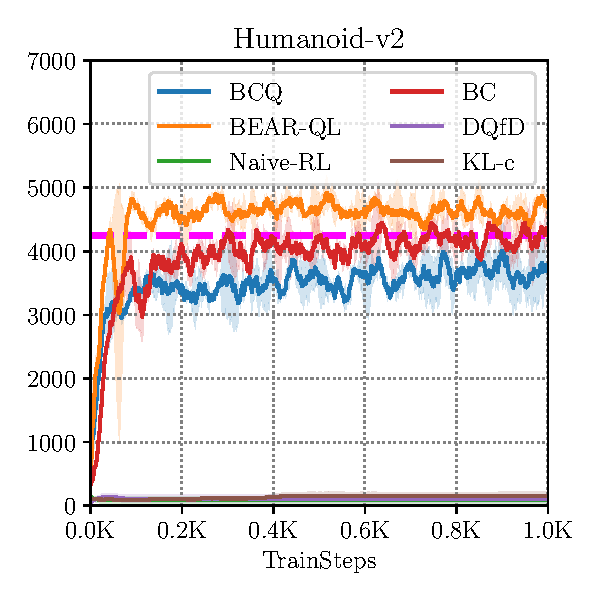
\includegraphics[width=0.4\linewidth]{chapters/bear/images/images_camera_ready/humanoid_mediocre_camera_ready.pdf}
       ~
        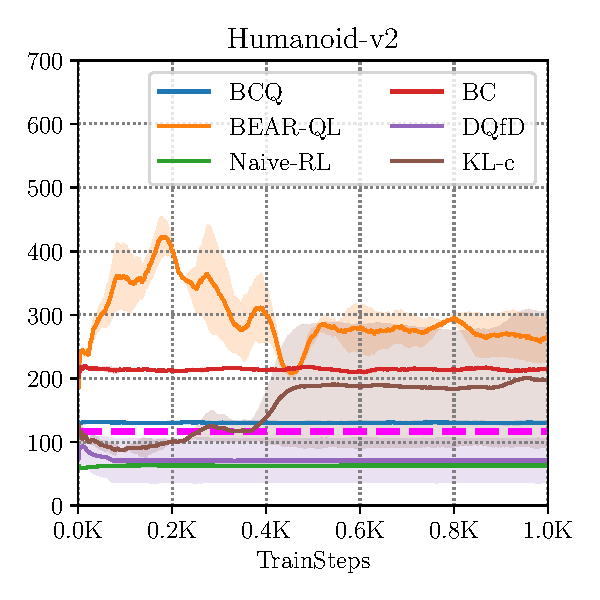
\includegraphics[width=0.4\linewidth]{chapters/bear/images/images_camera_ready/humanoid_random_camera_ready.pdf}
      \caption{\label{fig:humanoid} \footnotesize Performance of BEAR, BCQ, Na\"ive RL and BC on medium-quality (left) and random (right) data in the Humanoid-v2 environment. Note that BEAR outperforms prior methods.}
\end{figure}

%With random data, BCQ is expected to not perform well, as it constrains actions to the actions seen in the dataset at a particular state. On the other hand, a na\"ive off-policy RL algorithm is expected to perform well in these settings. In Figure~\ref{fig:optimal_random}, we show that BEAR outperforms \cite{fujimoto2018off} drastically while still performing comparable to the na\"ive RL algorithm in HalfCheetah-v2, and Hopper-v2, and outperforming it on Walker2d-v2 and Ant-v2 tasks. On optimal data, as the suboptimality bias is small, the best solution is to imitate the behavior policy. BEAR learns to imitate the behavior policy, and maintains stably there. In this setting, na\"ive-RL algorithm fails to learn (and mostly converges to the minimum possible reward, that can be obtained in the environment). Overall, BEAR is robust to the dataset composition, and can consistently perform in all settings -- mediocre, random and optimal data. Figure~\ref{fig:optimal_random} summarizes the average evaluation return of the learned policy as a function of training steps.

% show that DQNs are empirically less stable than off-policy actor critic algorithms(TD3). In all cases, note that BCQ~\cite{fujimoto18addressing} often ends up imitating the baseline, which explains the reason for poor performance on random data, and fast convergence to optimal performance on optimal data. However, the versatility of BEAR demonstrates its use as a practical algorithm irrespective of the quality of the dataset $\dataset$. We also examine the amount of deviation from the true MC-returns of the actor and the learned estimate of the Q-value, which again suggests that BEAR can learn reliable estimates of Q-values without excessive overestimation as observed in TD3, while achieving better expected return performance over BCQ. \TODO{Q vs MC figure left}

\begin{figure}
    \centering
    \begin{subfigure}[t]{0.23\textwidth}
        \centering
        % 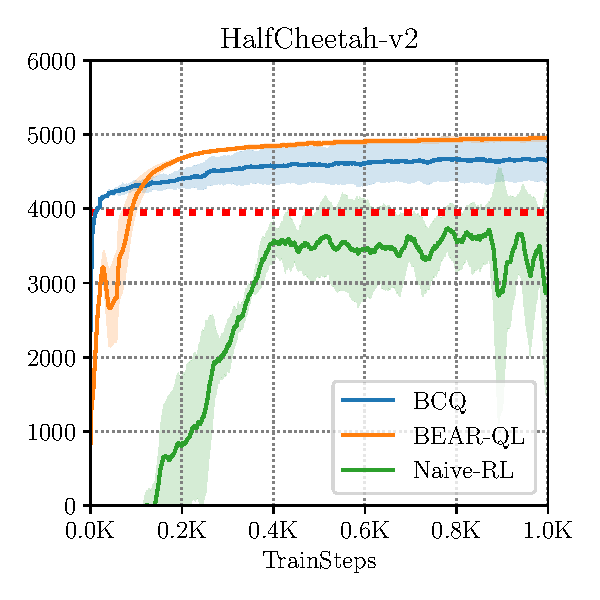
\includegraphics[width=0.99\linewidth]{chapters/bear/images/cheetah_mediocre_final.pdf}
        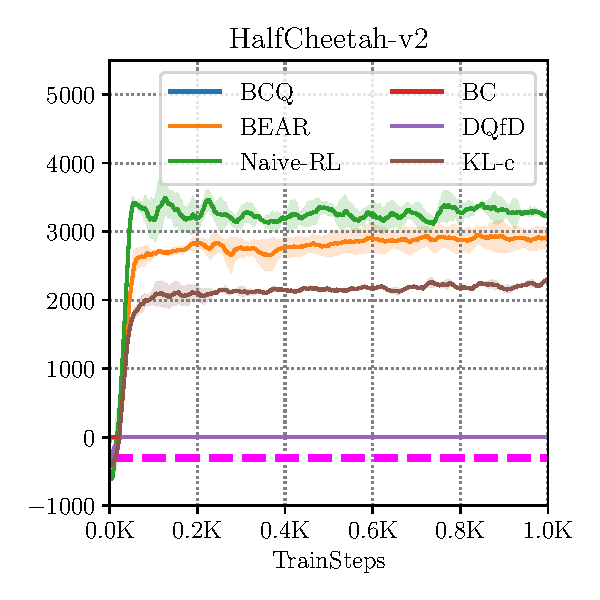
\includegraphics[width=0.99\linewidth]{chapters/bear/images/images_camera_ready/cheetah_random_final_camera_ready.pdf}
        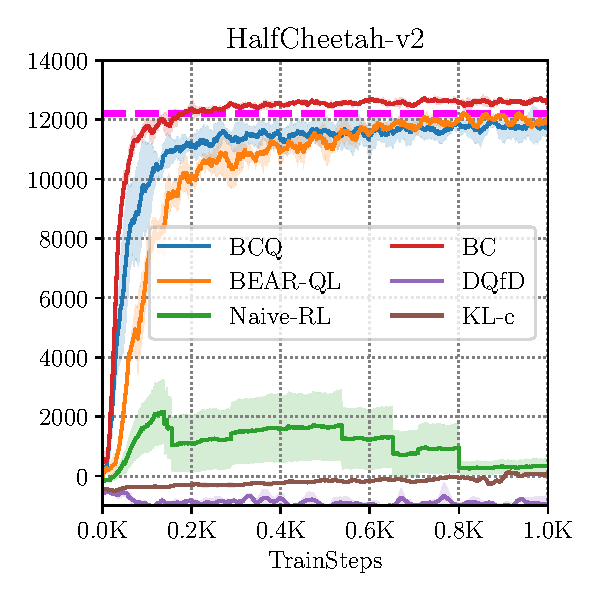
\includegraphics[width=0.99\linewidth]{chapters/bear/images/images_camera_ready/cheetah_optimal_camera_ready_new.pdf}
        % \caption{}
    \end{subfigure}%
    ~ 
    \begin{subfigure}[t]{0.23\textwidth}
        \centering
        % 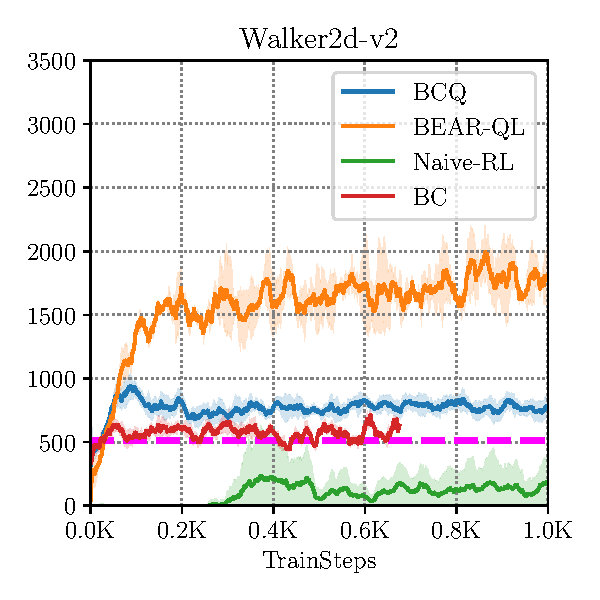
\includegraphics[width=0.99\linewidth]{chapters/bear/images/walker_mediocre_final.pdf}
        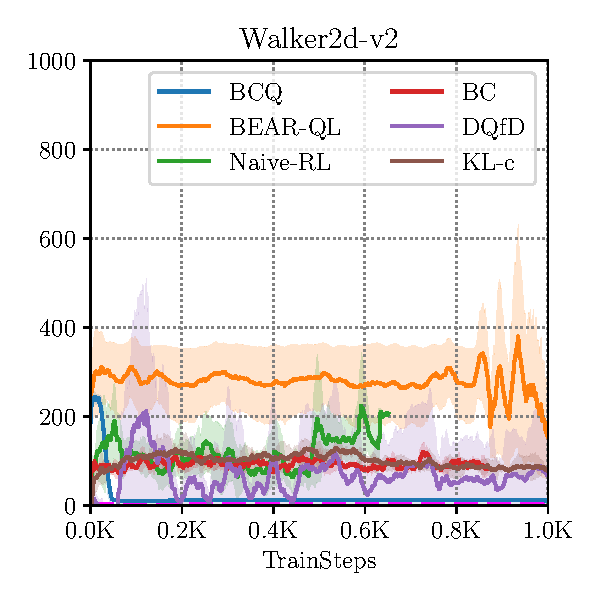
\includegraphics[width=0.99\linewidth]{chapters/bear/images/images_camera_ready/walker_random_camera_ready.pdf}
        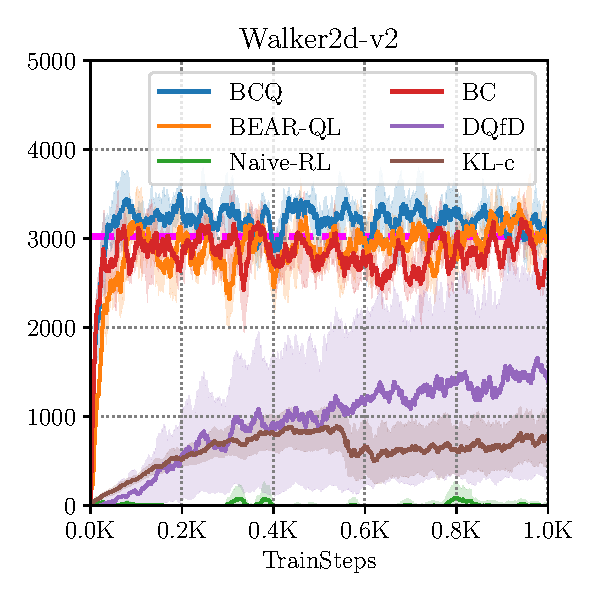
\includegraphics[width=0.99\linewidth]{chapters/bear/images/images_camera_ready/walker_optimal_camera_ready.pdf}
        % \caption{}
    \end{subfigure}
    ~
    \begin{subfigure}[t]{0.23\textwidth}
        \centering
        % 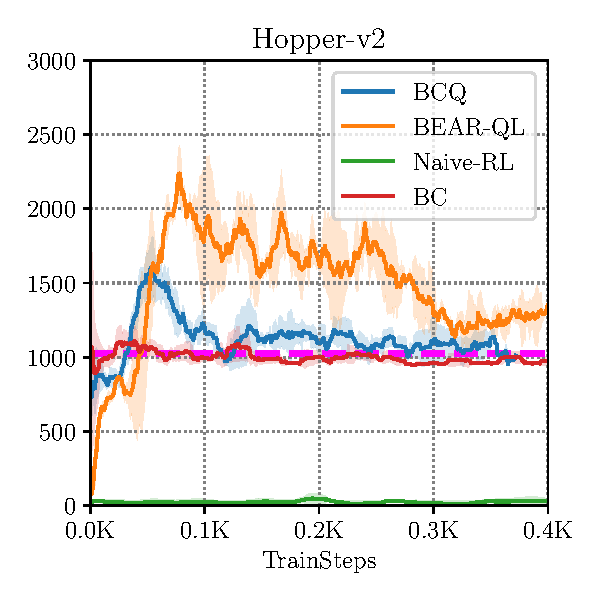
\includegraphics[width=0.99\linewidth]{chapters/bear/images/hopper_mediocre_final.pdf}
        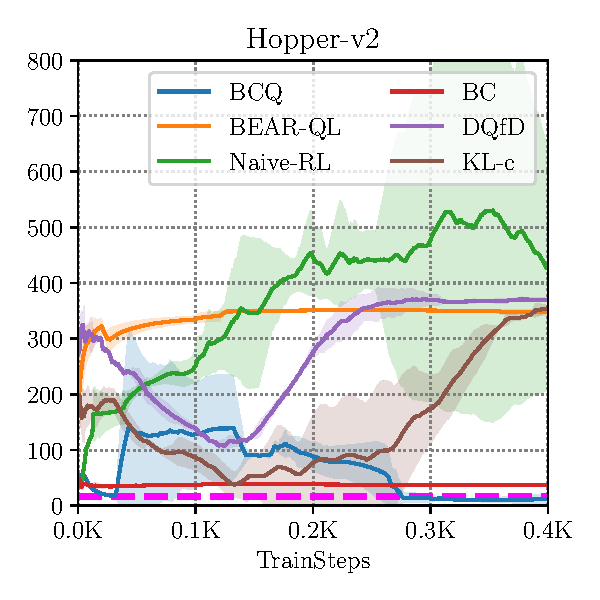
\includegraphics[width=0.99\linewidth]{chapters/bear/images/images_camera_ready/hopper_random_camera_ready.pdf}
        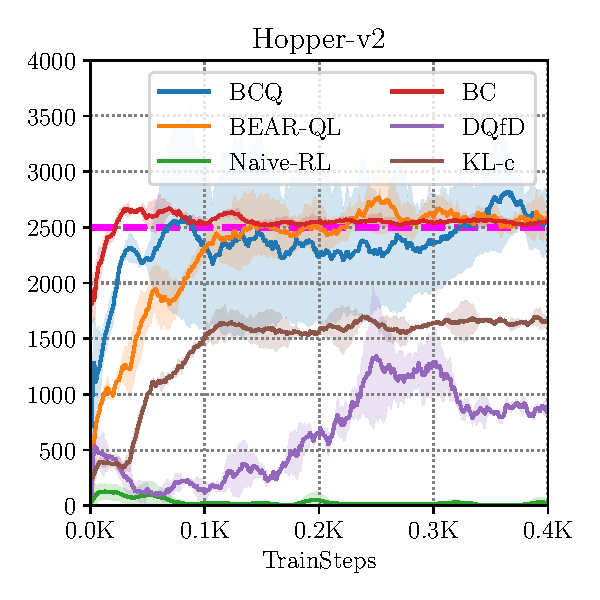
\includegraphics[width=0.99\linewidth]{chapters/bear/images/images_camera_ready/hopper_optimal_camera_ready.pdf}
        % \caption{}
    \end{subfigure}
    ~
    \begin{subfigure}[t]{0.23\textwidth}
        \centering
        % 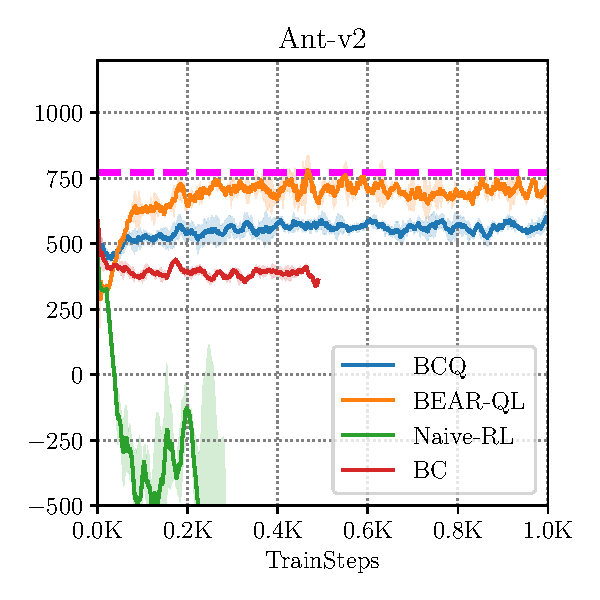
\includegraphics[width=0.99\linewidth]{chapters/bear/images/ant_mediocre_final.pdf}
        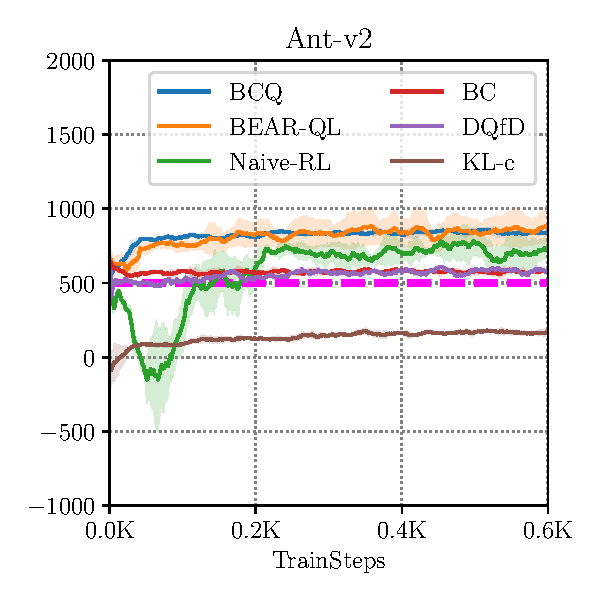
\includegraphics[width=0.99\linewidth]{chapters/bear/images/images_camera_ready/ant_random_camera_ready.pdf}
        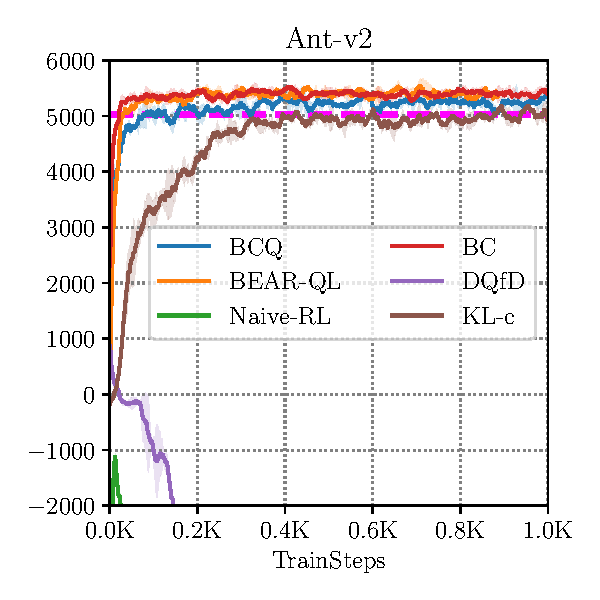
\includegraphics[width=0.99\linewidth]{chapters/bear/images/images_camera_ready/ant_optimal_camera_ready.pdf}
        % \caption{}
    \end{subfigure}
    \caption{\label{fig:optimal_random} \footnotesize Average performance of BEAR, BCQ, Na\"ive RL and BC on random data (top row) and optimal data (bottom row) over 5 seeds. BEAR is the only algorithm capable of learning in both scenarios. Na\"{i}ve RL cannot handle optimal data, since it does not illustrate mistakes, and BCQ favors a behavioral cloning strategy (performs quite close to behavior cloning in most cases), causing it to fail on random data. Average return over the training dataset is indicated by the dashed magenta line.}
\end{figure}

% \begin{figure*}[t!]
% \vspace{-0.1in}
%     \centering
%     \begin{subfigure}[t]{0.23\textwidth}
%         \centering
%         % 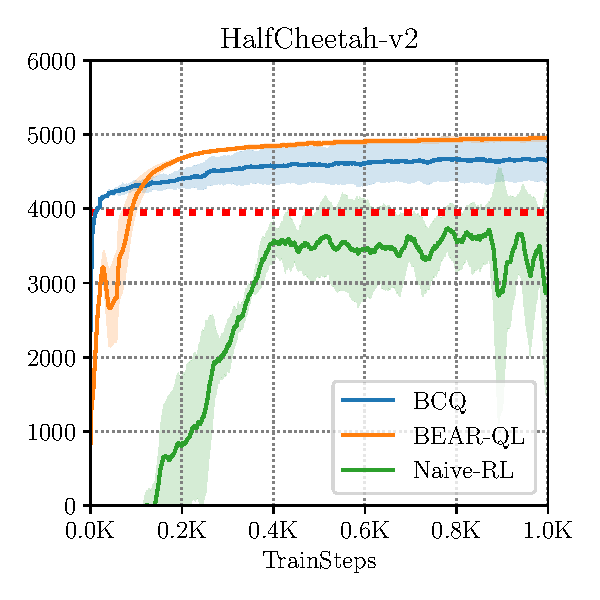
\includegraphics[width=0.99\linewidth]{chapters/bear/images/cheetah_mediocre_final.pdf}
%         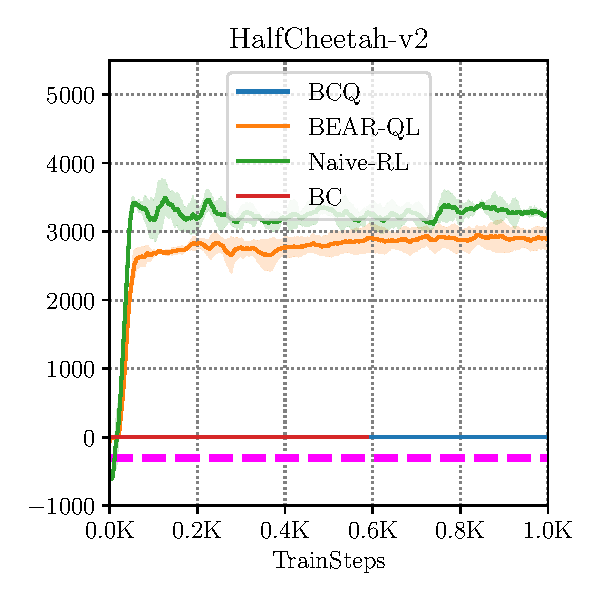
\includegraphics[width=0.99\linewidth]{chapters/bear/images/cheetah_random_final.pdf}
%         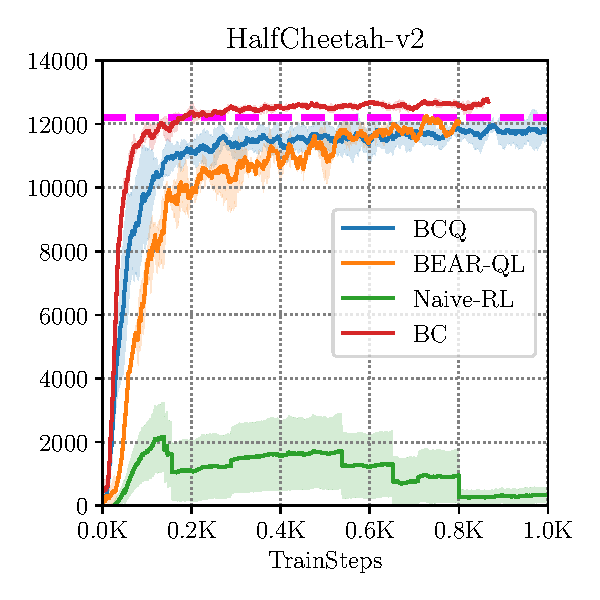
\includegraphics[width=0.99\linewidth]{chapters/bear/images/cheetah_optimal_final.pdf}
%         % \caption{}
%     \end{subfigure}%
%     ~ 
%     \begin{subfigure}[t]{0.23\textwidth}
%         \centering
%         % 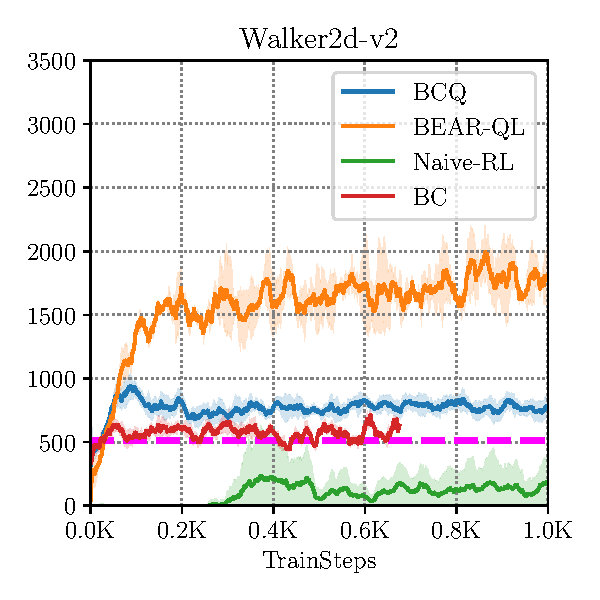
\includegraphics[width=0.99\linewidth]{chapters/bear/images/walker_mediocre_final.pdf}
%         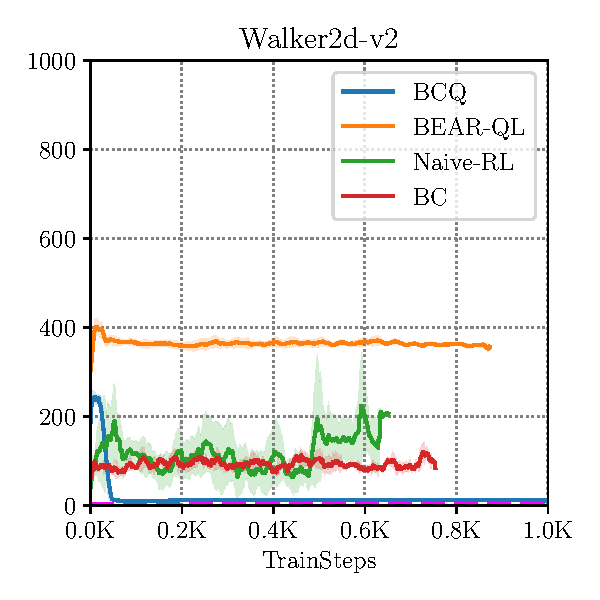
\includegraphics[width=0.99\linewidth]{chapters/bear/images/walker_random_final.pdf}
%         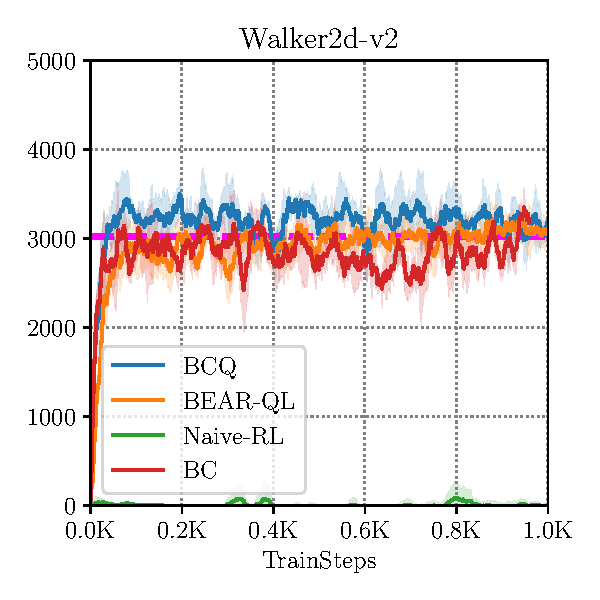
\includegraphics[width=0.99\linewidth]{chapters/bear/images/walker_optimal_final.pdf}
%         % \caption{}
%     \end{subfigure}
%     ~
%     \begin{subfigure}[t]{0.23\textwidth}
%         \centering
%         % 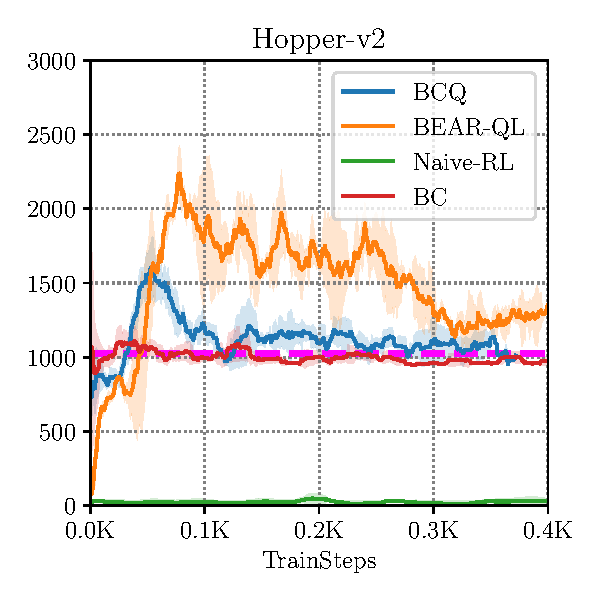
\includegraphics[width=0.99\linewidth]{chapters/bear/images/hopper_mediocre_final.pdf}
%         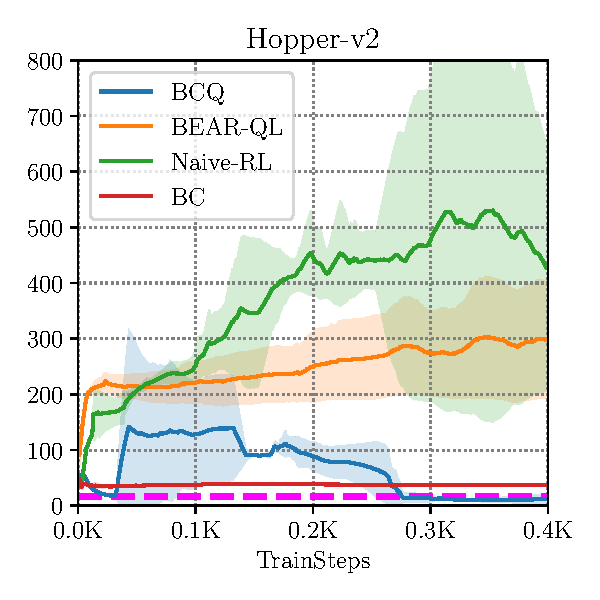
\includegraphics[width=0.99\linewidth]{chapters/bear/images/hopper_random_final.pdf}
%         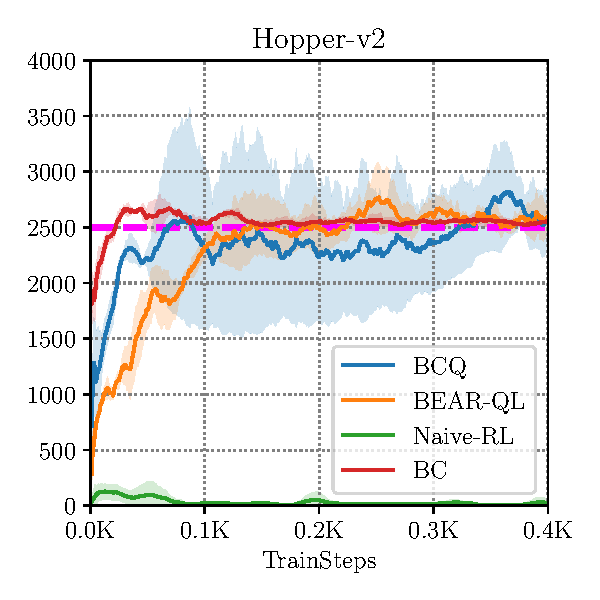
\includegraphics[width=0.99\linewidth]{chapters/bear/images/hopper_optimal_final.pdf}
%         % \caption{}
%     \end{subfigure}
%     ~
%     \begin{subfigure}[t]{0.23\textwidth}
%         \centering
%         % 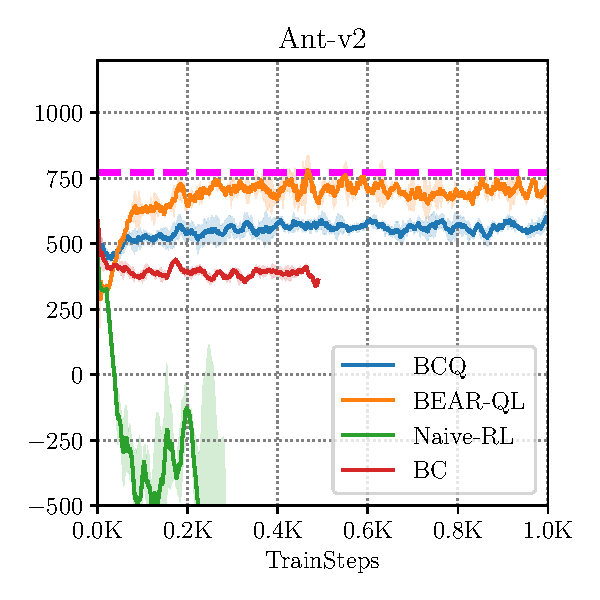
\includegraphics[width=0.99\linewidth]{chapters/bear/images/ant_mediocre_final.pdf}
%         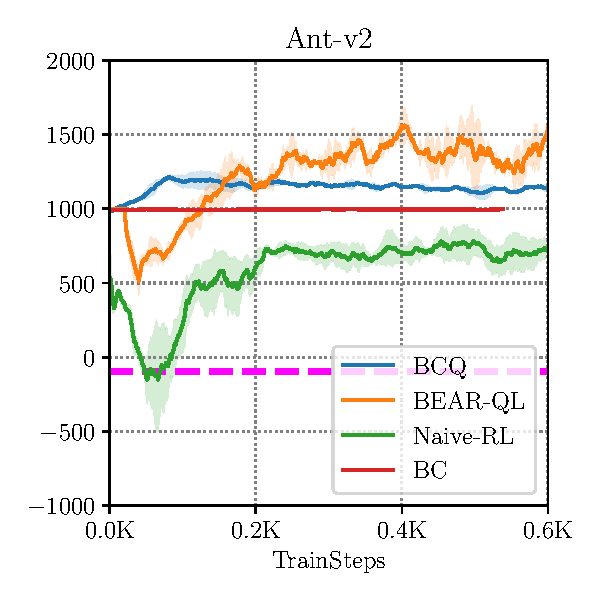
\includegraphics[width=0.99\linewidth]{chapters/bear/images/ant_random_final.pdf}
%         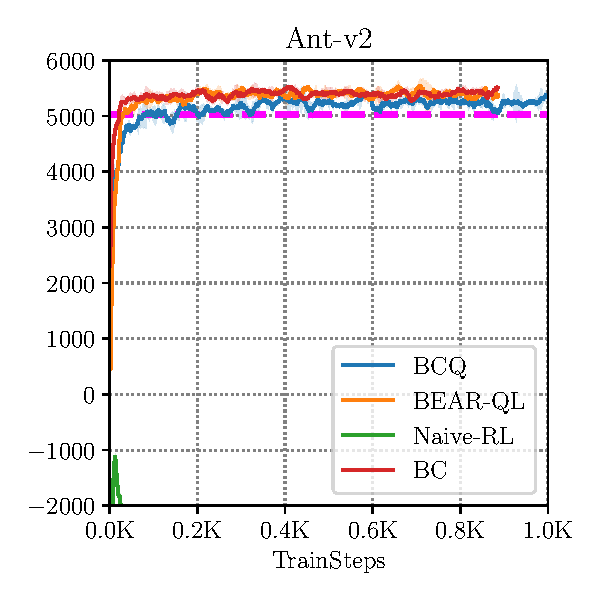
\includegraphics[width=0.99\linewidth]{chapters/bear/images/ant_optimal_final.pdf}
%         % \caption{}
%     \end{subfigure}
%     \caption{\footnotesize Average performance of BEAR, BCQ, Na\"ive RL and BC on random data (top row) and optimal data (bottom row) over 5 seeds. BEAR is the only algorithm capable of learning in both scenarios. Na\"{i}ve RL cannot handle optimal data, since it does not illustrate mistakes, and BCQ favors a behavioral cloning strategy (performs quite close to behavior cloning in most cases), causing it to fail on random data. Average return over the training dataset is indicated by the dashed magenta line.}
%     \label{fig:optimal_random}
%     \vspace{-0.1in}
% \end{figure*}

% \begin{figure*}[t!]
%     \centering
%     \begin{subfigure}[t]{0.31\textwidth}
%         \centering
%         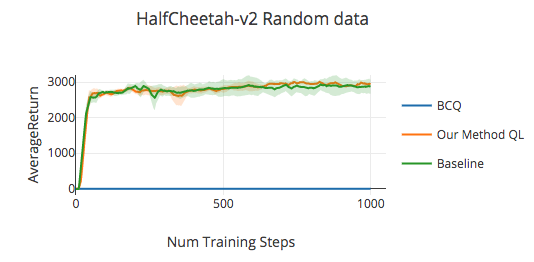
\includegraphics[width=0.99\linewidth]{chapters/bear/images/random_halfcheetah.png}
%         \caption{ }
%     \end{subfigure}%
%     ~ 
%     \begin{subfigure}[t]{0.31\textwidth}
%         \centering
%         \includegraphics[width=0.99\linewidth]{chapters/bear/images/mediocre_walker.png}
%         \caption{ }
%     \end{subfigure}
%     ~
%     \begin{subfigure}[t]{0.31\textwidth}
%         \centering
%         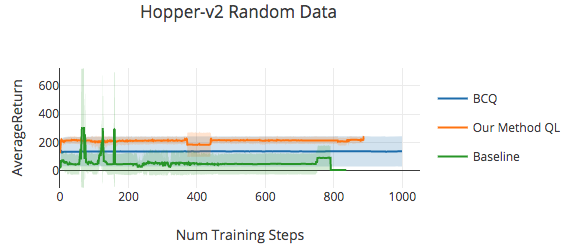
\includegraphics[width=0.99\linewidth]{chapters/bear/images/random_hopper.png}
%         \caption{ }
%     \end{subfigure}
%     \caption{Random Data}
% \end{figure*}

% \begin{figure*}[t!]
%     \centering
%     \begin{subfigure}[t]{0.23\textwidth}
%         \centering
%         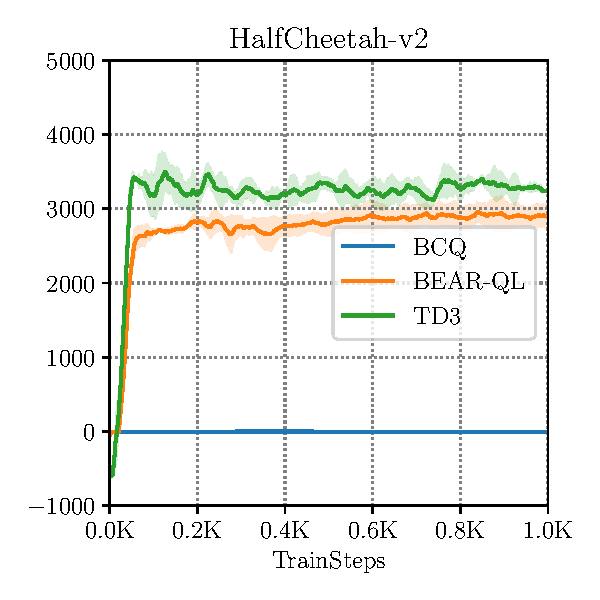
\includegraphics[width=0.99\linewidth]{chapters/bear/images/cheetah_random.pdf}
%         \caption{ }
%     \end{subfigure}%
%     ~ 
%     \begin{subfigure}[t]{0.23\textwidth}
%         \centering
%         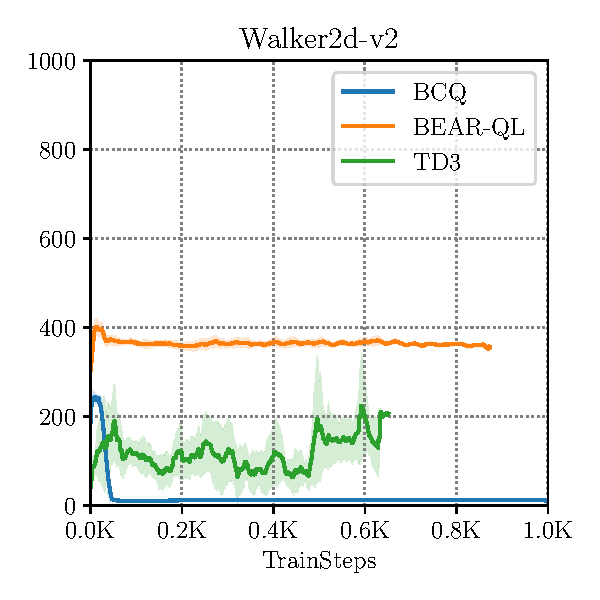
\includegraphics[width=0.99\linewidth]{chapters/bear/images/walker_random.pdf}
%         \caption{ }
%     \end{subfigure}
%     ~
%     \begin{subfigure}[t]{0.23\textwidth}
%         \centering
%         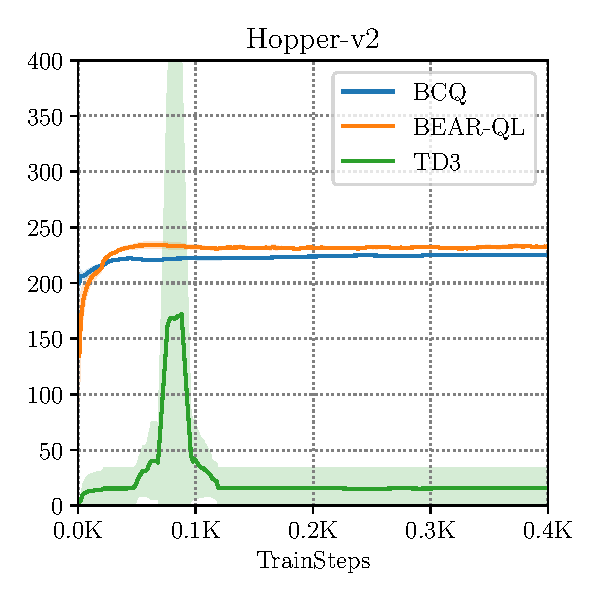
\includegraphics[width=0.99\linewidth]{chapters/bear/images/hopper_random.pdf}
%         \caption{ }
%     \end{subfigure}
%     ~
%     \begin{subfigure}[t]{0.23\textwidth}
%         \centering
%         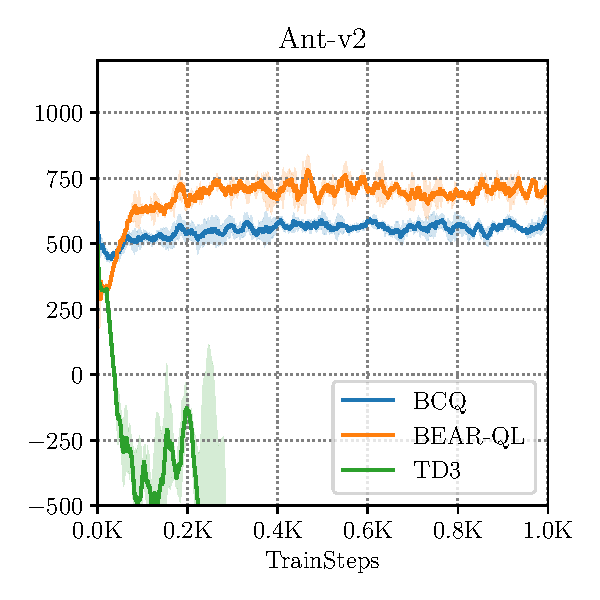
\includegraphics[width=0.99\linewidth]{chapters/bear/images/ant_mediocre.pdf}
%         \caption{ }
%     \end{subfigure}
%     \caption{Random Data}
% \end{figure*}

% \begin{figure*}[t!]
%     \centering
%     \begin{subfigure}[t]{0.23\textwidth}
%         \centering
%         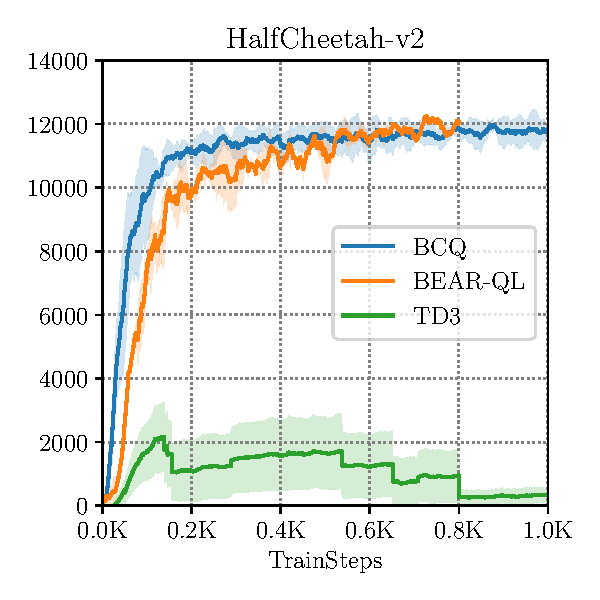
\includegraphics[width=0.99\linewidth]{chapters/bear/images/cheetah_optimal.pdf}
%         \caption{ }
%     \end{subfigure}%
%     ~ 
%     \begin{subfigure}[t]{0.23\textwidth}
%         \centering
%         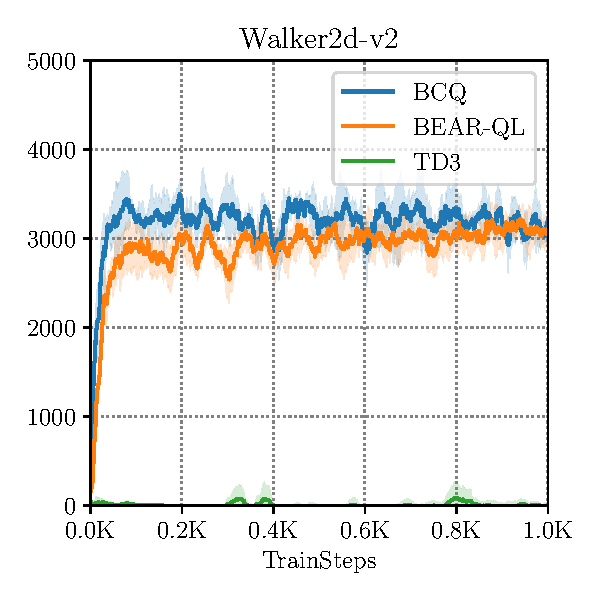
\includegraphics[width=0.99\linewidth]{chapters/bear/images/walker_optimal.pdf}
%         \caption{ }
%     \end{subfigure}
%     ~
%     \begin{subfigure}[t]{0.23\textwidth}
%         \centering
%         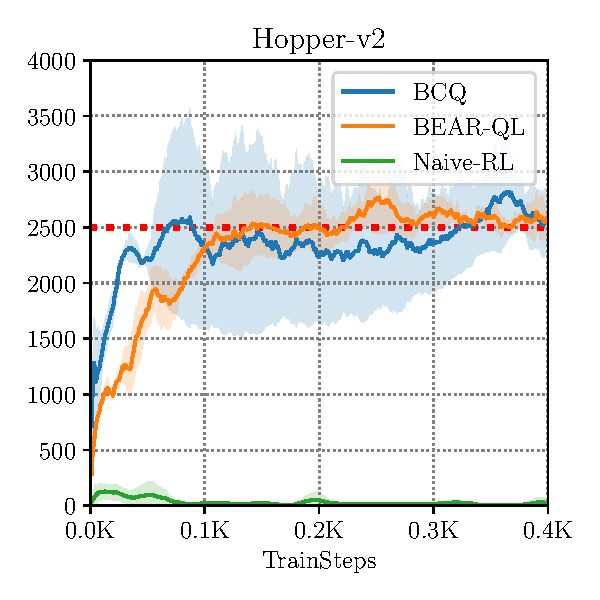
\includegraphics[width=0.99\linewidth]{chapters/bear/images/hopper_optimal.pdf}
%         \caption{ }
%     \end{subfigure}
%     ~
%     \begin{subfigure}[t]{0.23\textwidth}
%         \centering
%         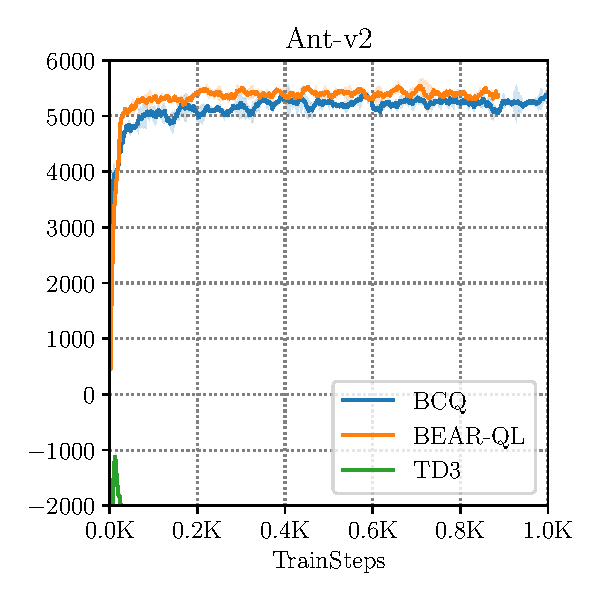
\includegraphics[width=0.99\linewidth]{chapters/bear/images/ant_optimal.pdf}
%         \caption{ }
%     \end{subfigure}
%     \caption{Optimal Data}
% \end{figure*}

\iffalse

\vspace{-5pt}
\subsection{Analysis of BEAR}
\label{subsec:ablations}
In this section, we aim to analyze different components of our method via an ablation study. Our first ablation studies the support constraint discussed in Section~\ref{sec:bear}, which uses MMD to measure support. We replace it with a more standard KL-divergence distribution constraint, which measures similarity in density. 
% \TODO{how is this done if we don't have the behavior policy? do you assume access for this study? -- we train a behavior policy on the data and then constrain to that with KL or MMD (so it should be a fair comparison)}
Our hypothesis is that this should provide a more conservative constraint, since matching distributions is not necessary for matching support. KL-divergence performs well in some cases, such as with optimal data, but as shown in Figure~\ref{fig:ablations}, it performs worse than MMD on medium-quality data. Even when KL-divergence is hand tuned fully, so as to prevent instability issues it still performs worse than a not-well tuned MMD constraint. We provide the results for this setting in the Appendix. We also vary the number of samples $n$ that are used to compute the MMD constraint. We find that smaller n ($\approx$ 4 or 5) gives better performance. Although the difference is not large, consistently better performance with 4 samples leans in favour of our hypothesis that an intermediate number of samples works well for support matching, and hence is less restrictive.

\fi
% Next, we study whether using a conservative Q-value estimate by subtracting the variance in the ensemble helps with learning. As shown in Figure~\ref{fig:ablations}, the conservative estimate 
%  makes a comparatively smaller difference than the use of MMD, providing some benefit on one task, while somewhat hurting performance on another.
% The ensemble produces more conservative estimates, which can result in underestimation in practice, and prevent overestimation divergence.

%The third factor in the ablation study is whether the usage of conservative estimates of Q-values subtracting the variance of the $Q$-ensemble helps. We find that on Hopper, usage of ensembles helps, whereas on Walker2d using ensembles hurts as the algorithm tends to underestimate Q-values. Figure~\ref{subfig:ensembles_ablation} demonstrates the average trend on 2 environments -- Hopper and Walker.




% \subsection{Generalization performance on datasets collected using a mixture of markovian policies.}
% We finally test our BEAR method in the case where the dataset $\dataset$ cannot be generated by a \TODO{Sergey and George: What's your opinion on having this section about non-markovian policies? This was one reason why Fujimoto got rejected. {https://openreview.net/forum?id=S1zlmnA5K7\&noteId=HJeQ-p0F2Q} }
% \TODO{Exp List: - Ant multiple + Point Mass multiple
%                 - with BCQ, BEAR, BEAR with n=1, BEAR without ensemble}

% \begin{figure}
%     \centering
%     \includegraphics{}
%     \caption{Caption}
%     \label{fig:my_label}
% \end{figure}
% \section{Discussion and Future Work}
\vspace{-5pt}
The goal in our work was to study off-policy reinforcement learning with static datasets. We theoretically and empirically analyze how error propagates in off-policy RL due to the use of out-of-distribution actions for computing the target values in the Bellman backup. Our experiments suggest that this source of error is one of the primary issues afflicting off-policy RL: increasing the number of samples does not appear to mitigate the degradation issue (Figure~\ref{fig:divergence}), and training with na\"{i}ve RL on data from a random policy, where there are no out-of-distribution actions, shows much less degradation than training on data from more focused policies (Figure~\ref{fig:optimal_random}). Armed with this insight, we develop a method for mitigating the effect of out-of-distribution actions, which we call BEAR-QL. BEAR-QL constrains the backup to use actions that have non-negligible support under the data distribution, but without being overly conservative in constraining the learned policy. We observe experimentally that BEAR-QL achieves good performance across a range of tasks, and across a range of dataset compositions, learning well on random, medium-quality, and expert data.

% \vspace{-0.15in}
\begin{wrapfigure}{r}{0.51\textwidth}
        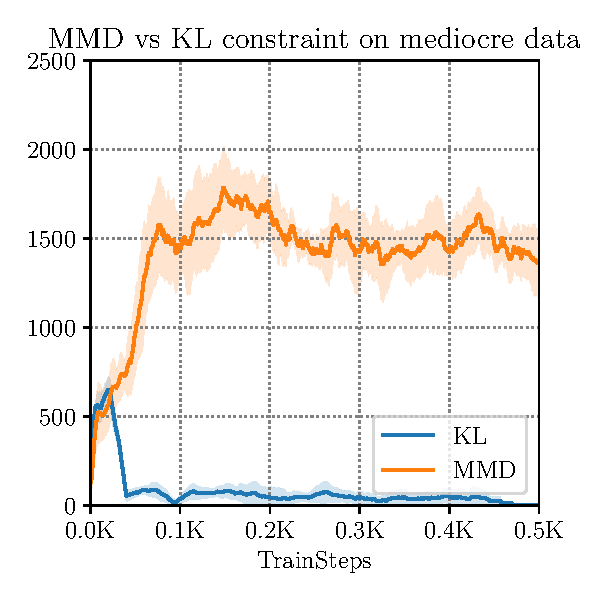
\includegraphics[width=0.48\linewidth]{chapters/bear/images/kl_vs_mmd_ablation_final.pdf}
       ~
        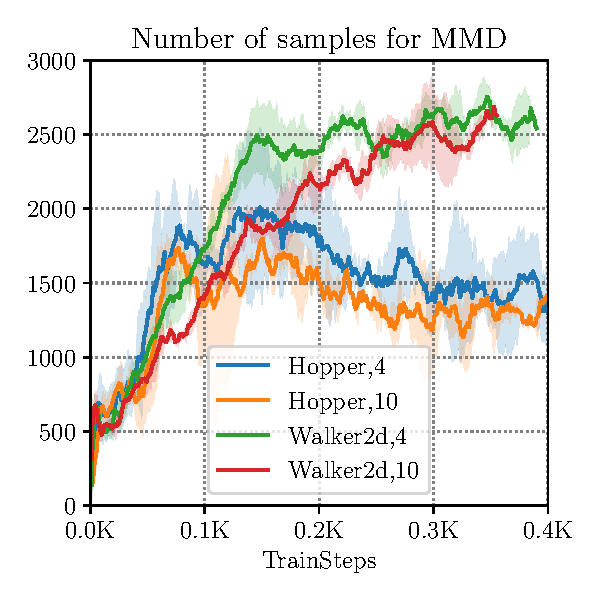
\includegraphics[width=0.48\linewidth]{chapters/bear/images/num_samples_ablation.pdf}
        % ~
        % \includegraphics[width=0.31\linewidth]{images/ensembles_ablation_final.pdf}
      \caption{\footnotesize Average return (averaged Hopper-v2 and Walker2d-v2) as a function of train steps for ablation studies from Section~\ref{subsec:ablations}. (a) MMD constrained optimization is more stable and leads to better returns, (b) 4 sample MMD is more performant than 10.}
    %   and (c) Ensemble variance has mixed benefit.}
      \label{fig:ablations}
\vspace{-10pt}
\end{wrapfigure}

While BEAR-QL substantially stabilizes off-policy RL, we believe that this problem merits further study. One limitation of our current method is that, although the learned policies are more performant than those acquired with na\"{i}ve RL, performance sometimes still tends to degrade for long learning runs. An exciting direction for future work would be to develop an early stopping condition for RL, perhaps by generalizing the notion of validation error to reinforcement learning. {A limitation of approaches that perform constrained-action selection is that they can be overly conservative when compared to methods that constrain state-distributions directly, especially with datasets collected from mixtures of policies. We leave it to future work to design algorithms that can directly constrain state distributions. A theoretically robust method for support matching efficiently in high-dimensional continuous action spaces is a question for future research. Perhaps methods from outside RL, predominantly used in domain adaptation, such as using asymmetric f-divergences~\citep{wu19domain} can be used for support restriction.} Another promising future direction is to examine how well BEAR-QL can work on large-scale off-policy learning problems, of the sort that are likely to arise in domains such as robotics, autonomous driving, operations research, and commerce. If RL algorithms can learn effectively from large-scale off-policy datasets, reinforcement learning can become a truly data-driven discipline, benefiting from the same advantage in generalization that has been seen in recent years in supervised learning fields, where large datasets have enabled rapid progress in terms of accuracy and generalization~\cite{imagenet_cvpr09}.

\section*{Acknowledgements}
We thank Kristian Hartikainen for sharing implementations of RL algorithms and for help in debugging certain issues. We thank Matthew Soh for help in setting up environments. We thank Aurick Zhou, Chelsea Finn, Abhishek Gupta, Kelvin Xu and Rishabh Agarwal for informative discussions. We thank Ofir Nachum for comments on an earlier draft of this paper. We thank Google, NVIDIA, and Amazon for providing computational resources. This research was supported by Berkeley DeepDrive, JPMorgan Chase \& Co., NSF IIS-1651843 and IIS-1614653, the DARPA Assured Autonomy program, and ARL DCIST CRA W911NF-17-2-0181.

% Q-learning methods are a common class of algorithms used in reinforcement learning (RL). However, their behavior with function approximation, especially with neural networks, is poorly understood theoretically and empirically. In this work, we aim to experimentally investigate potential issues in Q-learning, by means of a "unit testing" framework where we can utilize oracles to disentangle sources of error. 
% Specifically, we investigate questions related to function approximation, sampling error and nonstationarity, and where available, verify if trends found in oracle settings hold true with deep RL methods.
% We find that large neural network architectures have many benefits with regards to learning stability; offer several practical compensations for overfitting; and develop a novel sampling method based on explicitly compensating for function approximation error that yields fair improvement on high-dimensional continuous control domains. 

% \vspace{-0.4cm}
% \begin{AIbox}{\large{\textbf{Abstract}}}
% \vspace{4mm}
% In this chapter, we seek to understand challenges in the offline RL problem setting. To this end, we empirically study the behavior of off-policy RL methods when only training on a static, offline dataset. In principle, off-policy RL methods such as those based on approximate dynamic programming should succeed at leveraging experience collected from prior policies for sample-efficient learning. However, as we illustrate in this chapter, in practice, commonly used off-policy methods based on Q-learning and actor-critic are incredibly sensitive to \emph{both} the dataset distribution and quantity. Building on the insights from our empirical observations, we identify two main issues with learning value functions in the offline setting: \emph{distributional shift} and \emph{sampling error}. Later, we also demonstrate that these challenges also inhibit performance for other classes of off-policy RL methods such as model-based approaches. Finally, in subsequent chapters, we develop techniques to handle distributional shift, progressing towards reliable and easy-to-use offline RL algorithms.  
% \vspace{2mm}
% \end{AIbox}
    
% \vspace{-0.2cm}
\section{Introduction}
\vspace{-0.2cm}

In principle, off-policy reinforcement learning (RL) methods from Chapter~\ref{chapter:problem_statement} provide an effective way to learn optimal policies from static data: by learning value-functions, Q-learning and actor-critic algorithms, can learn optimal policies from even sub-optimal offline data. By attempting to isolate practical problems that hinder the usability of off-policy RL methods in learning from entirely static data, we wish to highlight challenges in offline RL. Specifically, we focus on answering the following questions: 

% Q-learning algorithms, which are based on approximating state-action value functions, are an efficient and commonly used class of RL methods. Q-learning methods have several very appealing properties: they are relatively sample-efficient when compared to policy gradient methods, and they allow for off-policy learning. This makes them an appealing choice for a wide range of tasks, from robotic control~\citep{kalashnikov18} and video game AI~\citep{Mnih2015} to off-policy learning from historical data for recommender systems~\citep{shani2005recommender}. However, although the basic tabular Q-learning algorithm is convergent and admits theoretical analysis~\cite{suttonrlbook}, its counterpart with function approximation is poorly understood. 
% In this paper, we aim to investigate the degree to which potential issues with Q-learning manifest in practice. 
% We empirically analyze aspects of the Q-learning method in a \emph{unit testing} framework, where we can employ oracle solvers to obtain ground truth Q-functions and distributions for exact analysis. We investigate the following questions:

% \textbf{1) What is the effect of function approximation on convergence?}
% Many practical RL problems require function approximation to handle large or continuous state spaces. However, the behavior of Q-learning methods under function approximation is not well understood -- there are simple counterexamples where the method diverges~\citep{Baird1995}. 
% To investigate these problems, we study the convergence behavior of Q-learning methods with function approximation by varying the function approximator power and analyzing the quality of the solution found. 
% We find, somewhat surprisingly, that divergence rarely occurs, and that function approximation error is not a major problem in Q-learning algorithms when the function approximator is powerful. This makes sense in light of the theory: a high-capacity approximator can perform an accurate projection of the bellman Backup, thus mitigating potential convergence issues due to function approximation. (Section~\ref{sec:function_approx})


\niparagraph{\large{(1) What is the effect of distributional shift?}}

% The standard formulation of off-policy Q-learning and actor-critic prescribes an update rule, with no corresponding objective function~\citep{Sutton09b}. This results in a learning process which optimizes an objective that suffers from distributional shift: the target values computed by the Bellman backup query actions from the learned policy, which is not necessarily identical to the data collection policy (and in general, we would expect that the learned policy would differ greatly from the data collection policy since it is supposed to improve over the behaviors in the offline dataset). We perform controlled experiments to investigate the amount of distributional shift and its impact on performance, observing that deviating away from the distributions of states and actions in the offline dataset can lead to significant instability over the course of learning.

The standard formulation of Q-learning and actor-critic prescribes a learning procedure that must make accurate counterfactul predictions about on states and actions visited by the learned policy. In general, the distribution of the learned policy will always be very different from that of the behavioral policy, and the difference will only be exacerbated for a correctly functioning algorithm that is able to find a policy close to the optimal policy for the problem. We perform controlled experiments to investigate the amount of distributional shift and its impact on performance, observing that deviating away from the distributions of states and actions in the offline dataset can lead to significant instability over the course of learning.



\niparagraph{\large{(2) What is the effect of sampling error?}}

In general, it is impossible to precisely infer the true underlying dynamical system using just a finite amount of offline data. This means that akin to standard supervised learning, off-policy RL algorithms that reuse a static dataset for learning would also overfit to the training data. To what extent, does this overfitting hurt performance? We experimentally show that overfitting exists in practice by performing ablation studies on the number of gradient steps utilized for learning, and by demonstrating that oracle based early stopping techniques can be used to improve performance of Q-learning algorithms.
%Thus, in our experiments we quantify the amount of overfitting which happens in practice, incorporating a variety of metrics, and performing a number of ablations and investigate methods to mitigate its effects.


% \textbf{4) What is the best sampling or weighting distribution?}
% Deeply tied to the distribution shift problem is the choice of which distribution to sample from. Do moving distributions cause instability, as Q-values trained on one distribution are evaluated under another in subsequent iterations?
% Researchers have often noted that on-policy samples are typically superior to off-policy samples~\citep{suttonrlbook}, and there are several theoretical results that highlight favorable convergence properties under on-policy samples. However, there is little theoretical guidance on how to pick distributions so as to maximize learning. To this end, we investigate several choices for the sampling distribution. {Surprisingly, we find that on-policy training distributions are not always preferable, and that broader, higher-entropy distributions often perform better, regardless of distributional shift. Motivated by our findings, we propose a novel weighting distribution, adversarial feature matching (AFM), which is explicitly compensates for function approximator error, while still producing high-entropy sampling distributions.}


%%AK: say this para in some different way
% In summary, we introduce a unit testing framework for Q-learning to disentangle potential bottlenecks where approximate components are replaced by oracles. This allows for controlled analysis of different sources of error. We study various sources of instability and error in Q-learning algorithms on tabular domains, and show that many of these trends hold true in high dimensional domains. We then propose a novel sampling distribution that improve performance even on high-dimensional tasks. %Our overall aim is to offer practical guidance for designing RL algorithms, as well as to identify important issues to solve in future research.

% % \section{Preliminaries}
\label{sec:backrgound}
Q-learning algorithms aim to solve a Markov decision process (MDP) by learning the optimal state-action value function, or Q-function. We define an MDP as a tuple $(\mathcal{S}, \mathcal{A}, \trans, R, \gamma)$. $\mathcal{S}, \mathcal{A}$ represent the state and action spaces, respectively. $\trans(s' | s, a)$ and $R(s,a)$ represent the dynamics (transition distribution) and reward function, respectively, and $\gamma \in (0,1)$ represents the discount factor. Letting $\rho_0(s)$ denote the initial state distribution, the goal in RL is to find a policy $\pi(a|s)$ that maximizes the expected cumulative discounted rewards, known as the \textit{returns}:
 $\pi^* = \argmax{\pi} E_{s_0 \sim \rho_0, s_{t+1} \sim \trans, a_t \sim \pi}\left[\sum_{t=0}^\infty \gamma^t R(s_t, a_t)\right] $
The quantity of interest in many Q-learning methods are the optimal state ($V^*(s)$) and state-action ($Q^*(s,a)$) value functions, which give the expected future return of the optimal policy starting from a particular state or state-action pair. Q-learning algorithms are based on iterating the Bellman backup operator $\backup$, defined as
\begin{align*}
(\backup Q)(s, a) &= R(s, a) + \gamma E_{s' \sim \trans}[V(s')]\\
V(s) &= \max_{a'} Q(s, a')
\end{align*}
Q-iteration is a dynamic programming algorithm that iterates the Bellman backup $Q^{t+1} \leftarrow \backup Q^t$. Because the Bellman backup is a $\gamma$-contraction in the $\linfnorm$ norm, and $Q^*$ is its fixed point, Q-iteration can be shown to converge to $Q^*$~\citep{suttonrlbook}. A deterministic optimal policy can then be obtained as $\pi^*(s) = \textrm{argmax}_{a} Q^*(s,a)$.

When state spaces are large, function approximation is needed to represent the Q-values. This corresponds to \textit{fitted Q-iteration} (FQI)~\citep{Ernst05}, a form of approximate dynamic programming (ADP), which forms the basis of modern deep RL methods such as DQN~\citep{Mnih2015}.
FQI projects the values of the Bellman backup onto a family of Q-function approximators $\Qclass$: $Q^{t+1} \leftarrow \Projmu(\backup Q^t)$.
$\Projmu$ denotes a $\mu$-weighted $\ltwonorm$ projection, which minimizes the \textit{Bellman error} via supervised learning:
\begin{equation}
\label{eqn:bellman_projection} 
\Projmu(Q) \defeq 
\argmin{Q' \in \Qclass} E_{s,a \sim \mu}[(Q'(s,a) - Q(s,a))^2]
 .\end{equation}
The values produced by the Bellman backup, $(\backup Q^t)(s,a)$ are commonly referred to as \textit{target values}, and when neural networks are used for function approximation, the previous Q-function $Q^t(s,a)$ is referred to as the \textit{target network}. In this work, we distinguish between the cases when the Bellman error is estimated with Monte-Carlo sampling or computed exactly (see Section~\ref{sec:setup_algos}). The sampled variant corresponds to FQI as described in the literature~\citep{Ernst05,Riedmiller2005}, while the exact variant is an example of conventional ADP methods~\citep{Bertsekas96}. 
Convergence guarantees for Q-iteration do not cleanly translate to FQI. $\Projmu$ is an $\ltwonorm$ projection, but $\backup$ is a contraction in the $\linfnorm$ norm -- this norm mismatch means the composition of the backup and projection is no longer guaranteed to be a contraction under any norm~\citep{Bertsekas96}, and hence convergence is not guaranteed.

A related branch of Q-learning methods are \textit{online Q-learning} methods,
in which Q-values are updated while samples are being collected in the MDP. This includes classic algorithms such as Watkin's Q-learning~\citep{Watkins1992}. Online Q-learning methods can be viewed as a form of stochastic approximation applied to Q-iteration and FQI~\citep{Bertsekas96}, and share many of its theoretical properties~\citep{tsitsiklis1994asynchronous,szepesvari1998asymptotic}.
Modern deep RL algorithms such as DQN~\citep{Mnih2015} have characteristics of both online Q-learning and FQI -- using replay buffers means the sampling distribution $\mu$ changes very little between target updates (see Section~\ref{sec:distr_shift}), and target networks are justified from the viewpoint of FQI. Because FQI corresponds to the case when the sampling distribution is static between target updates, the behavior of modern deep RL methods more closely resembles FQI than a true online method without target networks.


% \vspace{-0.2cm}
\section{Experimental Setup}
\label{sec:diagnosing_setup}
\vspace{-0.2cm}
% Our experimental setup is centered around \emph{unit-testing}. We evaluate a spectrum of Q-learning algorithms, starting with exact dynamic programming and replacing exact components with practical approximations, until the algorithm resembles modern deep Q-learning methods. 
% %We then introduce a suite of tabular environments where oracle solutions can be computed, to aid in diagnosis, as well as testing in high-dimensional environments to verify our hypotheses.

While it is definitely possible to study challenges with off-policy RL methods in offline RL on common deep RL benchmark tasks (e.g., OpenAI Gym~\citep{gym} environments), these tasks do not necessarily provide us with the ability to compute oracle solutions and isolate challenges individually. Therefore, we perform our study in a ``unit-testing'' setup, consisting of gridworld and other tabular environments with varying difficulty levels, where it is possible to compute oracle solutions and control for different factors independently.
% We release this suite of tasks at: \url{https://github.com/justinjfu/diagnosing_qlearning}.    


% \iffalse

% \subsection{Algorithms}
% \label{sec:setup_algos}
% We use three different Q-learning variants, each of which controls for a specific source of approximation error -- 
% Exact-FQI, Sampling-FQI, and Replay-FQI. 
% We use FQI as a basis for our controlled analysis, as it strongly resembles modern deep RL algorithms while allowing us to separately isolate target values, update rates, and the number of samples used for each iteration. We then confirm that the observed trends hold with several state-of-the-art deep RL methods (SAC~\citep{Haarnoja2017}, TD3~\citep{pmlr-v80-fujimoto18a}) on standard benchmark problems.
% %Although FQI is not exactly identical to commonly used deep RL methods, such as DQN~\citep{Mnih2015}, DDPG~\citep{Lillicrap2015},TD3~\citep{pmlr-v80-fujimoto18a}, and SAC~\citep{Haarnoja2017}, it is structurally similar and, when the replay buffer for the commonly used methods becomes large, the difference becomes negligible, since the sampling distribution changes very little between target network updates. 
% %However, FQI methods are much more amenable for controlled analysis, since we can separately isolate target values, update rates, and the number of samples used for each iteration. We therefore use variants of FQI as the basis for our analysis, but we also confirm that similar trends hold with more commonly used algorithms on standard benchmark problems.

% \begin{figure*}[ttt!]
% \begin{small}
% \begin{minipage}[t]{0.33\linewidth}
% \begin{algorithm}[H]
% \small
% \caption{Exact-FQI}
% \label{alg:fqiexact}
% \begin{algorithmic}[1]
%     \STATE Initialize Q-value approximator $Q_\theta(s,a)$.
%     \FOR{step $t$ in \{1, \dots, N\}}
%         \item[]
%         \item[]
%         \item[]
%         \STATE Evaluate $Q_{\theta^t}(s,a)$ at all states.
%         \STATE Compute exact target values at all states. \\
%         $y(s,a) = r(s,a) + \gamma E_{s'}[ V_{\theta^t}(s')]$ 
%         \STATE Minimize projection loss with respect to $\mu$: \\
%         $\argmin{\theta} E_\mu[(Q_\theta(s,a) - y(s,a))^2]$
%     \ENDFOR
% \end{algorithmic}
% \end{algorithm}
% \end{minipage}
% \begin{minipage}[t]{0.33\linewidth}
% \begin{algorithm}[H]
% \small
% \caption{Sampled-FQI}
% \label{alg:fqisampled}
% \begin{algorithmic}[1]
%     \STATE Initialize Q-value approximator $Q_\theta(s,a)$.
%     \FOR{step $t$ in \{1, \dots, N\}}
%         \item[]
%         \item[]
%         \STATE \textdiff{Collect $M$ samples from $\mu$.}
%         \STATE Evaluate $Q_{\theta^t}(s,a)$ \textdiff{on samples.}
%         \STATE Compute sampled target values \textdiff{on samples.}\\
%         $\hat{y}_i = r_i + \gamma V_{\theta^t}(s'_i)$ 
%         \STATE Minimize projection loss with respect to \textdiff{samples}: \\
%         $ \argmin{\theta} \frac{1}{M}\sum_{i=1}^M (Q_\theta(s_i,a_i) - y_i)^2$
%     \ENDFOR
% \end{algorithmic}
% \end{algorithm}
% \end{minipage}
% \begin{minipage}[t]{0.33\linewidth}
% \begin{algorithm}[H]
% \small
% \caption{Replay-FQI}
% \label{alg:fqireplay}
% \begin{algorithmic}[1]
%     \STATE Initialize Q-value approximator $Q_\theta(s,a)$, \textdiff{replay buffer $\ReplayBuffer$}.
%     \FOR{step $t$ in \{1, \dots, N\}}
%         \STATE \textdiff{Collect $K$ online samples from $\mu$.}
%         \STATE \textdiff{Append online samples to buffer $\ReplayBuffer$.}
%         \STATE Collect $M$ samples from $\ReplayBuffer$.
%         %\STATE \textbf{Collect $K$ replay samples $(s_k, a_k, s'_k, r_k)$ from $\ReplayBuffer$}.
%         \STATE Evaluate $Q_{\theta^t}(s,a)$ on samples.
%         \STATE Compute sampled target values on samples\\
%         $\hat{y}_i = r_i + \gamma V_{\theta^t}(s'_i)$ 
%         \STATE Minimize projection loss with respect to samples: \\
%         $ \argmin{\theta} \frac{1}{M}\sum_{i=1}^M (Q_\theta(s_i,a_i) - y_i)^2$
%     \ENDFOR
% \end{algorithmic}
% \end{algorithm}
% \end{minipage}
% \end{small}
% \end{figure*}


% \textbf{Exact-FQI} (Algorithm~\ref{alg:fqiexact}): Exact-FQI uses known dynamics and reward functions and computes the backup and projection on all state-action tuples, without sampling error. We use Exact-FQI to study convergence, distribution shift (by varying weighting distributions on transitions), and function approximation in the absence of sampling error. 
% %Exact-FQI eliminates errors due to sampling states, and computing inexact, sampled backups.

% \textbf{Sampled-FQI} (Algorithm~\ref{alg:fqisampled}): Sampled-FQI is a special case of Exact-FQI,
% where the Bellman error is approximated with Monte-Carlo estimates from a sampling distribution $\mu$, and the Bellman backup is approximated with samples from the dynamics as $r(s,a) + \gamma \max_{a'}Q(s', a')$. We use Sampled-FQI to study effects of overfitting. Sampled-FQI incorporates errors arising from function approximation, sampling, and distribution shift.

% \textbf{Replay-FQI} (Algorithm~\ref{alg:fqireplay}): Replay-FQI is a special case of Sampled-FQI that uses a \textit{replay buffer}~\citep{lin1992replay},
% that saves past transition samples $(s, a, s', r)$, which are used for computing Bellman error. Replay-FQI strongle resembles DQN~\cite{Mnih2015}, but lacking the online updates that allow $\mu$ to change within an FQI iteration. 
% With large replay buffers, we expect the difference between Replay-FQI and DQN to be minimal as $\mu$ changes slowly.

% We additionally investigate the following choices of weighting distributions ($\mu$) for the Bellman error:
% %When sampling the Bellman error, these can be implemented by sampling directly from the distribution, or via importance sampling.

% \textbf{Unif$(s,a)$}: Uniform weights over state-action space. 
% %This is the weighting distribution typically used by dynamic programming algorithms, such as FQI.

% \textbf{$\pi(s,a)$}: The on-policy state-action marginal induced by $\pi$.

% \textbf{$\pi^*(s,a)$}: The state-action marginal induced by $\pi^*$.

% \textbf{Random$(s,a)$}: State-action marginal induced by executing uniformly random actions.

% \textbf{Prioritized$(s,a)$}: Weights Bellman errors proportional to $|Q(s,a)-\backup Q(s,a)|$. This is similar to prioritized replay~\citep{Schaul2015} with $\beta=0$.

% \textbf{Replay$(s,a)$} and \textbf{Replay10$(s,a)$}: Averaged state-action marginal of all policies (or the last 10) produced during training. This simulates sampling from a replay buffer. 

% \fi


For our study, we selected eight tabular domains, each with different qualitative attributes, including: gridworlds of varying sizes and observations, blind Cliffwalk~\citep{Schaul2015}, discretized Pendulum and Mountain Car based on OpenAI Gym~\citep{gym},
and a sparsely connected graph. We discuss each domain in detail below:

\begin{itemize}

\item \textbf{Gridworlds}. The Gridworld environment is an NxN grid with randomly placed walls. The reward is proportional to Manhattan distance to a goal state (1 at the goal, 0 at the initial position), and there is a 5\% chance the agent travels in a different direction than commanded. We vary two parameters: the size ($16 \times 16$ and $64 \times 64$), and the state representations. We use a one-hot representation, an (X, Y) coordinate tuple (represented as two one-hot vectors), and a random representation, a vector drawn from $\mathcal{N}(0, 1)^N$, where N is the width or height of the Gridworld. The random observation significantly increases the challenge of function approximation, as significant state aliasing occurs.

\item \textbf{Cliffwalk}: Cliffwalk is a toy example from \citet{Schaul2015}. It consists of a sequence of states, where each state has two allowed actions: advance to the next state or return to the initial state. A reward of 1.0 is obtained when the agent reaches the final state. Observations consist of vectors drawn from $\mathcal{N}(0, 1)^{16}$.

\item \textbf{InvertedPendulum and MountainCar}: InvertedPendulum and MountainCar are discretized versions of continuous control tasks found in OpenAI gym~\citep{gym}, and are based on problems from classical RL literature. In the InvertedPendulum task, an agent must swing up an pendulum and hold it in its upright position. The state consists of the angle and angular velocity of the pendulum. Maximum reward is given when the pendulum is upright. The observation consists of the $\sin$ and $\cos$ of the pendulum angle, and the angular velocity. In the MountainCar task, the agent must push a vehicle up a hill, but the hill is steep enough that the agent must gather momentum by swinging back and forth within a valley in order to reach the top. The state consists of the position and velocity of the vehicle.

\item \textbf{SparseGraph}: The SparseGraph environment is a 256-state graph with randomly drawn edges. Each state has two edges, each corresponding to an action. One state is chosen as the goal state, where the agent receives a reward of one.

\end{itemize}

\noindent In order to provide consistent metrics across domains, we normalize returns and errors involving Q-functions by the returns of the expert policy $\pi^*$ on each environment. 

% \subsection{Function Approximators}
% Throughout our experiments, we use 2-layer ReLU networks, denoted by a tuple $(N, N)$ where N represents the number of units in a layer. The ``Tabular'' architecture refers to the case when no function approximation is used. 

% \subsection{High-Dimensional Testing}

% In addition to diagnostic experiments on tabular domains, we also wish to see if the observed trends hold true on high-dimensional environments. Thus, we include experiments on continuous control tasks in the OpenAI Gym benchmark~\citep{gym} (HalfCheetah-v2, Hopper-v2, Ant-v2, Walker2d-v2). In continuous domains, computing the maximum over actions of the Q-value is difficult ($\max_a Q(s,a)$). A common choice in this case is to use an ``actor'' function to approximate $\arg\max_a Q(s,a)$~\cite{Lillicrap2015,pmlr-v80-fujimoto18a,Haarnoja18}. This approach resembles Replay-FQI, but using the actor network in place of the max.
%\vspace{-20pt}
% % \section{Function Approximation and Convergence}
\label{sec:function_approx}

%The first issue we investigate is the connection between function approximation and convergence properties.

%\subsection{Technical Background}
This interaction between approximation and convergence has been a long-studied topic in RL and ADP. In control theory, it is closely related to the problems of state-aliasing or interference~\citep{Farrell95}. \citet{Baird1995} introduces a counterexample in which Watkin's Q-learning with linear approximators causes unbounded divergence. However, several works have noted that divergence need not occur. \citet{munos2005erroravi,antos2008concentrability,farahmand2010error} address the norm-mismatch problem by showing convergence guarantees in $\lpnorm$-norms, at the price of introducing a \textit{concentrability coefficient} that worsens the error bound (and is potentially infinite for deterministic MDPs). In policy evaluation, \citet{Tsitsiklis1997} prove that on-policy TD-learning with linear approximators converges, and methods such as GTD~\citep{Sutton09b} and ETD~\citep{Sutton2016} have extended results to off-policy cases.
In the control scenario, convergent algorithms such as SBEED~\citep{Dai2018} and Greedy-GQ~\citep{Maei2010} have been developed. Concurrently to us,\citet{VanHesselt2018} experimentally find that unbounded divergence rarely occurs with DQN variants on Atari games. 

\subsection{How does function approximation affect convergence and solution suboptimality?}
The crucial quantities we wish to measure are a trend between function approximation and performance, and a measure for the bias in the learning procedure introduced by function approximation.
Using Exact-FQI with uniform weighting (to remove sampling error), we plot the returns of the learned policy, and the $\linfnorm$ error between $Q^*$ and the solution found by Exact-FQI ($\lim_{t \to \infty} (\Projmu \backup)^t Q^0$) and the projection of the optimal solution  ($\Projmu Q^*$) in Fig.~\ref{fig:function_approx}. $\Projmu Q^*$ represents the best solution within model class, in absence of bootstrapping error. Thus, the difference between FQI error and projection error represents the additional bias introduced by FQI (the \textit{inherent Bellman error} of the function class~\citep{munos2008finite}). This is the potential gap that can be improved via better algorithm design.

\begin{figure}
\vspace{-0.5cm}
\caption{\label{fig:function_approx} Normalized returns and Q-function error with function approximation, averaged across domains and seeds. Small architectures show a large gap between the solution found by FQI (FQI Error) and the best solution within model class (Project Error).}
\centering
\includegraphics[width=0.7\linewidth]{chapters/diagnosing_q/images/fig_1.pdf}
% generated by plot_doodad_exact_fqi.py:returns_qstar_vs_arch
% data_dir = east1//2019-01-18-newenv-exact-weighting
\vspace{-0.8cm}
\end{figure}

We first note the obvious trend that smaller architectures produce lower returns and converge to worse solutions. 
However, we also find that smaller architectures introduce significant bias in the \textit{learning process}, and there is a significant gap between the solution found by Exact-FQI and the best solution within the model class. 
One explanation is that when the target is bootstrapped, we must represent all Q-functions along the path to the solution, and not only the final result~\citep{Bertsekas96}.
This observation implies that using large architectures is crucial not only because they have capacity to represent a better solution, but also because they are easier to train using bootstrapping. 
We also note that divergence rarely occurs in practice, occuring in only 0.9\% of our experiments (measured as the Q-values growing larger than 10 times $Q^*(s,a)$). 

For high-dimensional problems, we present experiments on varying the architecture of the Q-network in SAC~\cite{Haarnoja18} in Appendix Fig.~\ref{fig:size_sac}. We still observe that large networks have the best performance, and that divergence rarely happens even in high-dimensional continuous spaces. We briefly discuss theoretical intuitions on apparent discrepancy between the lack of unbounded divergence in relation known counterexamples in Appendix~\ref{app:bounded_error}.

% \vspace{-0.2cm}
\section{Impact of Distributional Shift}
\label{sec:sampling_distributions}
\vspace{-0.2cm}

%As alluded to in Section~\ref{sec:analysis_nonstationarity}, the choice of sampling distribution $\mu$ is an important design decision can have a large impact on performance. Indeed, it is not immediately clear which distribution is ideal for Q-learning. In this section, we hope to shed some light on this issue.

%\subsection{Technical Background}
% Off-policy data has been cited as one of the ``deadly triads'' for Q-learning~\citep{suttonrlbook}, which has potential to cause instabilities in learning. On-policy distributions~\citep{Tsitsiklis1997} and fixed behavior distributions~\citep{Sutton09a,Maei2010} have often been targeted for theoretical convergence analysis, and many works use importance sampling to correct for off-policyness~\citep{precup2001offpol, munos2016safe}
% However, to our knowledge, there is relatively little guidance which compares how different weighting distributions compare in terms of convergence rate and final solutions.

% Off-policy RL methods applied to the offline RL problem would typically attempt to learn an optimal policy, even though the static dataset may not be generated from an optimal policy. As a result, one issue to emerge is that of \emph{distributional shift}: while these methods can only train a model of the value-function and the policy using state-action tuples from the data, these models  will need to make correct predictions on states and actions sampled from a different distribution encountered upon deployment. In general, models trained via machine learning are not robust when the distribution of inputs changes, indicating that distributional shift can be challenge for off-policy RL methods. Is distributional shift a challenge in offline RL?   

Off-policy RL methods applied to the offline RL problem would typically attempt to learn an optimal policy, even though the static dataset may not be generated from an optimal policy. As a result, one issue that emerges is that of \emph{distributional shift}: while these methods train a model of the value-function and the policy only using state-action tuples from the data, upon deployment, these models will need to make correct predictions on states and actions sampled from a different distribution of the learned policy. In general, models trained via machine learning are not robust when the distribution of inputs changes, indicating that distributional shift can be a challenge for off-policy RL methods. Is distributional shift a challenge in offline RL?

Indeed, theoretically, the effects of distributional shift have been quantified using the notion of a concentrability coefficient~\citep{munos2005erroravi}, a constant typically $\gg 1$, which provides a worst-case error bound on the performance of an off-policy RL method due to distributional shift. To evaluate if this challenge persists empirically as well, we will analyze Q-learning methods for various choices of data distributions in this section.

A crucial design decision we must make is to consider setups that do not confound distributional shift with access to limited data. Therefore, for our study, we provide the underlying algorithm oracle access to all state-action transitions in the MDP, but vary the \emph{distribution} over state-action pairs from which these transitions are sampled.

% Indeed, theoretically, the effects of distributional shift have been quantified using the notion of a concentrability coefficient~\citep{munos2005erroravi}, a constant typically $\ggt 1$, which provides a worst-case error bound on the performance of an off-policy RL method due to distributional shift. To evaluate if this challenge persists empirically as well, we will analyze Q-learning methods for various choices of data distributions in this section. 

% A crucial design decision we must make is to consider setups that do not confound distributional shift with access to limited data. Therefore, for our study, we provide the underlying algorithm oracle access to all state-action transitions in the MDP, but vary the \emph{distribution} over state-action pairs that these transitions are sampled according to.   
% ~\citep{NIPS2017_6913} suggests that when the state-distribution is fixed, the action distribution should be weighted by the optimal policy for residual Bellman errors. In deep RL, prioritized replay~\citep{Schaul2015}, and mixing replay buffer with on-policy data~\citep{hausknecht2016policy,zhang2018deeper} have been found to be effective. %We aim to empirically analyze multiple choices for weighting distributions to determine which are the most effective.

%\vspace{-10pt}
\vspace{-0.2cm}
\subsection{What Are the Best Data Distributions Without Sampling Error?}
\label{subsec:dist_shift_exact}
\vspace{-0.2cm}

% \begin{figure*}[ttt!]
% \begin{subfigure}{0.3\linewidth}
% \caption{\footnotesize \label{fig:distribution_shift_vs_returns} Average distribution shift across time for different data distributions, plotted against returns for a 256x256 model. We find that distribution shift does not have strong correlation with returns.}
% \includegraphics[width=0.99\columnwidth]{chapters/diagnosing_q/images/returns_vs_shift}
% % generated by plot_distribution_shift.py
% % data_dir = east1//2019-02-12-exact-weighting-distr-shift
% \vspace{-0.2in}
% \end{subfigure}
% ~\vline~
% \begin{subfigure}{0.3\linewidth}
% \caption{\footnotesize \label{fig:weighting_schemes} Weighting distribution versus architecture in Exact-FQI. Replay(s, a) consistently provides the highest performance. Note that Adversarial Feature Matching is comparable to Replay(s, a), but surprisingly better for small networks. }
% \includegraphics[width=0.99\columnwidth]{chapters/diagnosing_q/images/exact_fqi_schemes.pdf}
% % generated by plot_exact_weighting.py
% % data_dir = east1//2019-01-18-newenv-exact-weighting
% \vspace{-0.3in}
% \end{subfigure}
% ~\vline~
% \begin{subfigure}{0.3\linewidth}
% \caption{\footnotesize \label{fig:weighting_entropy_vs_returns} Normalized returns plotted against normalized entropy for different weighting distributions. All experiments use Exact-FQI with a 256x256 network. We see a general trend that high-entropy distributions lead to greater performance.}
% \includegraphics[width=0.99\columnwidth]{chapters/diagnosing_q/images/returns_vs_entropy}
% % generated by plot_distribution_shift.py
% % data_dir = east1//2019-02-12-exact-weighting-distr-shift
% \end{subfigure}
% \end{figure*}

\begin{wrapfigure}{r}{0.45\linewidth}
    \vspace{-0.2cm}
    \includegraphics[width=0.99\linewidth]{chapters/diagnosing_q/images/returns_vs_entropy}
    \caption{\footnotesize \label{fig:weighting_entropy_vs_returns} Normalized returns plotted against normalized entropy for different weighting distributions. All experiments assume access to all state-action pairs with a 256x256 Q-network. We see a general trend that high-entropy distributions lead to greater performance, corroborating the uniformity hypothesis.}
    \vspace{-0.2cm}
    % generated by plot_distribution_shift.py
    % data_dir = east1//2019-02-12-exact-weighting-distr-shift
\end{wrapfigure}
We begin by studying the effect of data distributions when disentangled from sampling error. We run Q-learning with an ablation over various Q-function network architectures and data distributions and report our aggregate results in Fig.~\ref{fig:weighting_entropy_vs_returns}. $\text{Unif}(\bs, \mathbf{a})$, $\text{Replay}(\bs, \mathbf{a})$ (using a replay buffer consisting of data from a mixture of policies with different degrees of optimality), and $\text{Prioritized}(\bs, \mathbf{a})$ (weighting induced by prioritized experience replay~\citep{Schaul2015}) consistently result in the highest returns across all architectures. On the other hand, relatively ``narrow'' data distributions, such as those induced the optimal policy ($\pi^*$) or only using a mixture of a few policies ($\text{Replay}(10)$) results in poor performance.
% We believe that these results are in favor of the \textit{uniformity} hypothesis: intuitively, the best distributions spread weight across larger support of the state-action space, reducing the amount of possible distributional shift. On the other hand, less-uniform distributions such as the state-action distirbution induced by the optimal policy, present multiple avenues to deviate away from the offline data distribution, resulting in larger distributional shift.
We believe that these results favor the \textit{uniformity} hypothesis: intuitively, the best distributions spread weight across a larger support of the state-action space, reducing the amount of possible distributional shift. On the other hand, less-uniform distributions, such as the state-action distribution induced by the optimal policy, present multiple avenues to deviate away from the offline data distribution, resulting in larger distributional shift.

\textbf{To summarize}, this indicates that narrow data distributions lead to worse performance compared to higher-entropy data distributions, indicating that distributional shift can have a significant impact on the performance of off-policy RL in the offline setting.
%These distributions generally result in the tightest contraction rates, and allow the Q-function to focus on high-error regions. 
%In the sampled setting, this observation motivates exploration algorithms that maximize state coverage (for example, ~\citet{hazan2018} solve an exploration objective which maximizes state-space entropy).
%However, note that in this particular experiment is distinct from exploration, as there is no sampling involved. 
%All states are observed, just with different weights, thus isolating the issue of distributions from the issue of sampling.
% \section{Question 2: What is the Impact of Sampling Error and Overfitting?}
\label{sec:overfitting}

%A second source of error in minimizing the Bellman error, orthogonal to function approximation, is that of sampling or generalization error. The next issue we investigate is the effect of sampling error on Q-learning methods.

%\subsection{Technical Background}

Thus far, we have observed that the performance of off-policy RL algorithms based on Q-learning can be quite sensitive to the distribution of the offline dataset, even when all the transition tuples in the MDP are provided to the algorithm and only the weighting over these samples is varied. In this section, we aim to study a distinct question: we study
\begin{wrapfigure}{r}{0.5\linewidth}
    \centering
    \vspace{-10pt}
    \includegraphics[scale=0.4]{chapters/diagnosing_q/images/samples_arch.pdf}
    \vspace{-0.2cm}
    \caption{\label{fig:sampling_256} Samples plotted with returns for a 256x256 network. More samples yields better performance.}
    \vspace{-0.5cm}
    %plot_sampling
    %east1//2019-01-20-newenv-sample-weighting
\end{wrapfigure}
\!\!the performance of off-policy Q-learning when the offline dataset is of a finite size, and may not contain all transitions in the MDP. To address any confounders from distributional shift, we provide the underlying Q-learning algorithm oracle access to collecting a limited amount of data from the current snapshot of the learned policy. While this sort of active data collection is not possible in the offline RL problem setting, we find that it allows us to more carefully localize the challenges of overfitting and sampling error.

% Approximate dynamic programming assumes that the projection of the Bellman backup (Eqn.~\ref{eqn:bellman_projection}) is computed exactly, but in reinforcement learning we can normally only compute the \textit{empirical Bellman error} over a finite set of samples. In the PAC framework, overfitting can be quantified by a bounded error in between the empirical and expected loss with high probability, which decays with sample size~\citep{Shalev2014}. \citet{munos2008finite, maillard2010finite, tosatto2017boosted} provide such PAC-bounds which account for sampling error in the context of Q-learning and value-based methods, and quantify the quality of the final solution in terms of sample complexity.

We analyze several key points that relate to sampling error. First, we show that Q-learning is prone to overfitting, and that this overfitting has a real impact on performance. 

\subsection{Quantifying Overfitting}
We first quantify the amount of overfitting that happens during training, by varying the number of samples. In order provide comparable validation errors across different experiments, we fix a reference sequence of Q-functions, $Q^1, ... , Q^N$, obtained during an arbitrary run of Q-learning. We then retrace the training sequence, and minimize the projection error $\Projmu(Q^t)$ at each training iteration, using varying amounts of on-policy data or sampling from a replay buffer. We measure the validation error (the expected Bellman error) at each iteration under the on-policy distribution, plotted in Figure~\ref{fig:sampling_validation_loss}. We note the obvious trend that more samples leads to significantly lower validation loss. 
% A more interesting observation is that sampling from the replay buffer results in the lowest on-policy validation loss, despite bias due to distribution mismatch from sampling off-policy data. As we elaborate in Section~\ref{sec:analysis_nonstationarity}, we believe that replay buffers are effective because they reduce overfitting and have good sample coverage over the state space, not necessarily due to reducing the effects of nonstationarity.

Next, Figure~\ref{fig:sampling_256} shows the relationship between number of samples and returns. We see that more samples leads to improved learning speed and a better final solution. A full sweep including architectures is presented in the Appendix (Figure~\ref{fig:sampling_arch_sweep}). Despite overfitting being an issue, larger architectures still perform better because the bias introduced by smaller architectures dominates. This observation indicate that the nature of overfitting in RL is likely significantly different from that of supervised learning: while overfitting in supervised learning can bne controlled by regulating model capacity, off-policy RL methods likely need to rely on alternative techniques to control overfitting. We have made some progress towards understanding this questions in \citet{li2022effective}.   

\begin{figure*}[ttt!]
\begin{subfigure}{0.31\linewidth}
\includegraphics[width=0.97\linewidth]{chapters/diagnosing_q/images/overfitting.pdf}
%plot_overfitting
%central1//2019-01-21-overfitting-coupled
\caption{\label{fig:sampling_validation_loss} On-policy validation losses for varying amounts of on-policy data (or replay buffer), averaged across environments and seeds. Note that sampling from the replay buffer has lower on-policy validation loss, despite bias from distribution shift.}
\end{subfigure}
~\vline~
\begin{subfigure}{0.31\linewidth}
\includegraphics[trim={0 0 7.0cm 0},clip,width=0.97\linewidth]{chapters/diagnosing_q/images/grad_steps_fqi}
%plot_overfitting
%central1//2019-01-21-overfitting-coupled
\caption{\label{fig:fqi_grad_sweep}Normalized returns plotted over training iterations (32 samples per iteration), for different ratios of gradient steps per sample. We observe that intermediate values of gradient steps work best, and too many gradient steps hurt performance.}
\end{subfigure}
~\vline~
\begin{subfigure}{0.31\linewidth}
\includegraphics[trim={0 0 4.4cm 0},clip,width=0.97\linewidth]{chapters/diagnosing_q/images/validation_stop}
%plot_validation_stop
%west1//2019-02-20-replay-validation-stop
\caption{\label{fig:validation_stop}Normalized returns plotted over training iterations (32 samples are taken per iteration), for different early stopping methods. We observe that using proper early stopping can result in a modest performance increase.}
\end{subfigure}
\end{figure*}

\subsection{Does Compensating for Overfitting Improve Performance?}

Finally, to confirm our hypotheses regarding overfitting, we now wish to understand if compensating for overfitting does lead to improved performance. One common technique for reducing overfitting is to utilize \textit{early stopping} methods to mitigate overfitting without reducing model size.
% We first note that the number of gradient steps taken per sample in the projection step has an important effect on performance -- too few steps and the algorithm learns slowly, but too many steps and the algorithm may initially learn quickly but overfit. To show this, we run an ablation over the number of gradient steps taken per sample in Replay-FQI and TD3 (TD3 uses 1 by default). Results for FQI are shown in Fig.~\ref{fig:fqi_grad_sweep}, and for TD3 in Appendix Fig.~\ref{fig:td3_grad_sweep}.
In order to understand whether early stopping criteria can reduce overfitting, we employ \emph{oracle} stopping rules to provide an ``upper bound'' on the best potential improvement. We try two criteria for setting the number of gradient steps: the expected Bellman error and the expected returns of the greedy policy (oracle returns). We implement both methods by minimizing the TD-error to convergence, and retroactively selecting the intermediate Q-function which is judged best by the evaluation metric. Using oracle stopping metrics results in a modest boost in performance in tabular domains (Fig.~\ref{fig:validation_stop}). Thus, we believe that there is promise in further improving such early-stopping methods for reducing overfitting in deep RL algorithms.

~

\textbf{To summarize}, we can draw a few conclusions from our experiments in this section. First, overfitting is indeed an issue with Q-learning, and too many gradient steps or too few samples can lead to poor performance. Second, although overfitting is a problem, large architectures are still preferred, because the bias from function approximation outweighs the increased overfitting from using large models. 

Finally, we also remark that attempting to learn optimal policies from a static offline dataset will present both distributional shift and overfitting challenges together, and we would expect these to be tightly coupled with each other in the following sense: the inability to correclty identify the underlying MDP from finite samples in the offline dataset will induce errors in policy optimization, and these errors would then be exacerbated in the next step of learning as the learned policy deviates from the training data. This will also be evident in the theoretical results that we will present in subsequent chapters.    
% \section{Non-Stationarity}
\label{sec:analysis_nonstationarity}

%In this section, we discuss issues related to the non-stationarity of the Q-learning process (relating to the Bellman backup and Bellman error minimization).

%\subsection{Technical Background}
Instability in Q-learning methods is often attributed to the nonstationarity of the objective \citep{Lillicrap2015,Mnih2015}. 
Nonstationarity occurs in two places: in the changing target values $\backup Q$, and in a changing weighting distribution $\mu$ (``distribution shift''). 
Note that a non-stationary objective, by itself, is not indicative of instability. For example, gradient descent can be viewed as successively minimizing linear approximations to a function: for gradient descent on $f$ with parameter $\theta$ and learning rate $\alpha$, we have the ``moving'' objective $\theta^{t+1} = \argmin{\theta}\{ \theta^T \nabla_\theta f(\theta^t) - \frac{1}{2\alpha} \normtt{\theta - \theta^t} \} = \theta^t - \alpha \nabla_\theta f(\theta^t)$. 
However, the fact that the Q-learning algorithm prescribes an update rule and not a stationary objective complicates analysis. Indeed, the motivation behind algorithms such as GTD~\citep{Sutton09a, Sutton09b}, approximate linear programming~\citep{de2002alp}, and residual methods~\citep{Baird1995,scherrer2010residual} can be seen as introducing a stationary objective that can be optimized with standard methods such as gradient descent.
%Therefore, a key question to investigate is whether these non-stationarities are detrimental to the learning process.
% \vspace{-25pt}

\subsection{Does a moving target cause instability in the absence of a moving distribution?}

To study the moving target problem, we first isolate the speed at which the target changes. To this end, we define the $\alpha$-smoothed Bellman backup, $\backup^\alpha$, which computes an exponentially smoothed update as follows: 
$\backup^{\alpha}Q = \alpha \backup Q + (1-\alpha)Q$.
% \vspace{-5pt}
This scheme is inspired by the soft target update used in algorithms such as DDPG~\citep{Lillicrap2015} and SAC~\citep{Haarnoja2017} to improve the stability of learning. Standard Q-iteration uses a ``hard'' update where $\alpha=1$. A soft target update weakens the contraction of Q-iteration from $\gamma$ to $1-\alpha+\alpha\gamma$ (see Appendix~\ref{app:alpha_smoothed_q}),
so we expect slower convergence, but perhaps it is more stable under heavy function approximation error. We performed experiments with this modified backup using Exact-FQI under the $\text{Unif}(s,a)$ weighting distribution.

Our results are presented in Appendix Fig.~\ref{fig:smooth_fqi}.
We find that the most cases, the hard update with $\alpha=1$ results in the fastest convergence and highest asymptotic performance. However, for smaller architectures, $4 \times 4$ and $16 \times 16$, lower values of $\alpha$ (such as 0.1) achieve slightly higher asymptotic performance. Thus, while more expressive architectures are still stable under fast-changing targets, we believe that a slowly moving target may have benefits under heavy approximation error. This evidence points to either using large function approximators, in line with the conclusions drawn in the previous sections, or slowing the target updates on problems with high approximation error.

\subsection{Does distribution shift impact performance?}
\label{sec:distr_shift}

\begin{figure}[tb]
\caption{\label{fig:distribution_shift_tv_loss} Distribution shift and loss shift plotted against time. Prioritized and on-policy distributions induce the greatest shift, whereas replay buffers greatly reduce the amount of shift.}
\includegraphics[width=0.51\columnwidth]{chapters/diagnosing_q/images/dist_shift_tv3.pdf}
\includegraphics[width=0.47\columnwidth]{chapters/diagnosing_q/images/dist_shift_loss_tv3.pdf}
% \vspace{-10pt}
% generated by plot_distribution_shift.py:plot_tv_loss_over_time
% data_dir = east1//2019-01-18-newenv-exact-weighting
\end{figure}


To study the distribution shift problem, we exactly compute the amount of distribution shift between iterations in total-variation distance, $D_{TV}(\mu^{t+1} || \mu^{t})$ and the ``loss shift'':
$\mathbb{E}_{\mu^{t+1}}[ (Q^{t} - \backup Q^{t})^2] - \mathbb{E}_{\mu^{t}}[ (Q^{t} - \backup Q^{t})^2]$.
The loss shift quantifies the Bellman error objective when evaluated under a new distribution - if the distribution shifts to previously unseen states, we would expect a highly inaccurate Q-value in such states, leading to high loss shift.

% \begin{figure}[ht]

% \end{figure}


We run our experiments using Exact-FQI with a 256x256 layer architecture, and plot the distribution discrepancy and the loss discrepancy in Fig.~\ref{fig:distribution_shift_tv_loss}. 
We find that Prioritized$(s,a)$ has the greatest shift, followed by on-policy variants. Replay buffers greatly reduce distribution shift compared to on-policy learning, which is similar to the de-correlation argument cited for its use by~\citet{Mnih2015}.
However, we find that this metric correlates little with the performance of FQI (Fig.~\ref{fig:distribution_shift_vs_returns}). For example, prioritized weighting performs well yet has high distribution shift.

Overall, our experiments indicate that nonstationarities in both distributions and target values, when isolated, do not cause significant stability issues. Instead, other factors such as sampling error and function approximation appear to have more significant effects on performance.
%Therefore, we investigate how to design a \emph{better} sampling distribution, without regard to nonstationarity, in the next section.
%In the light of these findings, we might therefore ask: can we design a \emph{better} sampling distribution, without regard for distributional shift and with regard for high-entropy, that results in better final performance, and is realizable in practice? We investigate this in the following section.



\niparagraph{\large{Model-Free Conservative Value Estimation}}

\section{Discussion of CQL Variants}
\label{app:cql_variants}
We derive several variants of CQL in Section~\ref{sec:framework}. Here, we discuss these variants on more detail and describe their specific properties. We first derive the variants: CQL($\mathcal{H}$), CQL($\rho$), and then present another variant of CQL, which we call CQL(var). This third variant has strong connections to distributionally robust optimization~\citep{namkoong2017variance}.

\textbf{CQL($\mathcal{H}$).} In order to derive CQL($\mathcal{H}$), we substitute $\mathcal{R} = \mathcal{H}(\mu)$, and solve the optimization over $\mu$ in closed form for a given Q-function. For an optimization problem of the form:
\begin{equation*}
    \max_{\mu}~~ \E_{\bx \sim \mu(\bx)}[f(\bx)] + \mathcal{H}(\mu)~~~ \text{s.t.}~~~ \sum_{\bx} \mu(\bx) = 1,~ \mu({\bx}) \geq 0~ \forall \bx,
\end{equation*}
the optimal solution is equal to $\mu^*(\bx) = \frac{1}{Z} \exp(f(\bx))$, where $Z$ is a normalizing factor. Plugging this into Equation~\ref{eqn:cql_framework}, we exactly obtain Equation~\ref{eqn:practical_objective}.

\textbf{CQL($\rho$).} In order to derive CQL($\rho$), we follow the above derivation, but our regularizer is a KL-divergence regularizer instead of entropy.
\begin{equation*}
    \small{\max_{\mu}~~ \E_{\bx \sim \mu(\bx)}[f(\bx)] + D_{\mathrm{KL}}(\mu || \rho)~~~ \text{s.t.}~~~ \sum_{\bx} \mu(\bx) = 1,~ \mu({\bx}) \geq 0~ \forall \bx}.
\end{equation*}
The optimal solution is given by, $\mu^*(\bx) = \frac{1}{Z} \rho(\bx) \exp(f(\bx))$, where $Z$ is a normalizing factor. Plugging this back into the CQL family (Equation~\ref{eqn:cql_framework}), we obtain the following objective for training the Q-function (modulo some normalization terms):
\begin{equation}
    \small{\min_{Q}~ \alpha \E_{\bs \sim d^\behavior(\bs)}\left[\E_{\mathbf{a} \sim \rho(\mathbf{a}|\bs)} \left[Q(\bs, \mathbf{a}) \frac{\exp(Q(\bs, \mathbf{a}))}{Z'}\right] - \E_{\mathbf{a} \sim \behavior(\mathbf{a}|\bs)}\left[Q(\bs, \mathbf{a})\right]\right] + \frac{1}{2}\!\E_{\bs, \mathbf{a}, \bs' \sim \mathcal{D}}\left[\left(Q - \bellman^{\policy_k} \hat{Q}^{k} \right)^2 \right]\!.}
    \label{eqn:cql_rho_objective}
\end{equation}

\textbf{CQL(var).} Finally, we derive a CQL variant that is inspired from the perspective of distributionally robust optimization (DRO)~\citep{namkoong2017variance}. This version penalizes the variance in the Q-function across actions at all states $\bs$, under some action-conditional distribution of our choice. In order to derive a canonical form of this variant, we invoke an identity from \citet{namkoong2017variance}, which helps us simplify Equation~\ref{eqn:cql_framework}. To start, we define the notion of ``robust expectation'': for any function $f(\bx)$, and any empirical distribution $\hat{P}(\bx)$ over a dataset $\{ \bx_1, \cdots, \bx_N\}$ of $N$ elements, the ``robust'' expectation defined by: 
\begin{equation*}
    R_N(\hat{P}) := \max_{\mu(\bx)} ~~\E_{\bx \sim \mu(\bx)}[f(\bx)] \text{~~~s.t.~~~} D_{f}(\mu(\bx), \hat{P}(\bx)) \leq \frac{\delta}{N},
\end{equation*}    
can be approximated using the following upper-bound:
\begin{equation}
    R_N(\hat{P}) \leq \E_{\bx \sim \hat{P}(\bx)}[f(\bx)] + \sqrt{\frac{2 \delta~ \text{var}_{\hat{P}(\bx)}(f(\bx))}{N}},
    \label{eqn:robust_expectation}
\end{equation}
where the gap between the two sides of the inequality decays inversely w.r.t. to the dataset size, $\mathcal{O}(1/N)$. By using Equation~\ref{eqn:robust_expectation} to simplify Equation~\ref{eqn:cql_framework}, we obtain an objective for training the Q-function that penalizes the variance of Q-function predictions under the distribution $\hat{P}$. 
\begin{multline}
    \min_{Q}~~ \frac{1}{2}~ \E_{\bs, \mathbf{a}, \bs' \sim \mathcal{D}}\left[\left(Q - \bellman^{\policy_k} \hat{Q}^{k} \right)^2 \right] + \alpha \E_{\bs \sim d^\behavior(\bs)}\left[\sqrt{\frac{\text{var}_{\hat{P}(\mathbf{a}|\bs)}\left( Q(\bs, \mathbf{a}) \right)}{d^\behavior(s) |\mathcal{D}|}} \right] \\ 
    + \alpha \E_{s \sim d^\behavior(\bs)}\left[ \E_{\hat{P}(\mathbf{a}|\bs)}[Q(\bs, \mathbf{a})] - \E_{\behavior(\mathbf{a}|\bs)}[Q(\bs, \mathbf{a})] \right]
    \label{eqn:variance_regularized_again}
\end{multline}
The only remaining decision is the choice of $\hat{P}$, which can be chosen to be the inverse of the empirical action distribution in the dataset, $\hat{P}(\mathbf{a}|\bs) \propto \frac{1}{\hat{D}(\mathbf{a}|\bs)}$, or even uniform over actions, $\hat{P}(\mathbf{a}|\bs) = \text{Unif}(\mathbf{a})$, to obtain this variant of variance-regularized CQL.

% \textbf{CQL with variable state distributions.} The formulations of CQL in Sections~\ref{sec:policy_eval} and \ref{sec:framework} only use a variable action distribution $\mu(\mathbf{a}|\bs)$. In principle, we can extend these formulations to account for a variable state-distribution as well. In order to do this, we can modify Equation~\ref{eqn:objective_1} as follows:
% \begin{multline}
%     \label{eqn:cql_framework_state_dist}
%     \small{\min_{Q} ~~ \alpha \E_{\bs \sim \textcolor{red}{\mu(\bs)}, \mathbf{a} \sim \textcolor{red}{\mu(\mathbf{a}|\bs)}}\left[Q(\bs, \mathbf{a})\right] + \frac{1}{2}~ \E_{\bs, \mathbf{a}, \bs' \sim \mathcal{D}}\left[\left(Q(\bs, \mathbf{a}) - \bellman^{\policy} \hat{Q}^{k} (\bs, \mathbf{a}) \right)^2 \right].}
% \end{multline}
% In this case, the resulting tabular Q-function iterate, $\hat{Q}^k$ is given by:
% \begin{equation*}
% \hat{Q}^{k+1}(\bs, \mathbf{a}) = \bellman^\policy \hat{Q}^k (\bs, \mathbf{a}) - \alpha \left[\frac{\mu(\bs) \mu(\mathbf{a}|\bs)}{d^\behavior(\bs) \behavior(\mathbf{a}|\bs)} - 1\right].
% \end{equation*}
% We note that analogous to Proposition~\ref{thm:cql_underestimates}, we can argue that this is a lower bound estimate, since a positive quantity (i.e. density ratios) is being subtracted from the ideal tabular Q-function backup, at each iteration.

\section{Discussion of Gap-Expanding Behavior of CQL Backups}
\label{app:gap_amplify}
\vspace{-0.25cm}
% now lets talk about the section that compares prior methods and CQL with function approximation in terms of action gap
%%SL.5.11: I wonder if it could make sense to have a single "Related Work and Connections to Policy Constraints" section, where we could have a subsection on "Related Prior Work" subsection on "Prior Work on Offline RL with Constraints" and "Comparative Analysis of CQL and Policy Constraint Methods" or something? Not certain about this, but maybe we try it and see how it looks? It's a bit unconventional...

% setup the stage, what we want to do in this section and why
In this section, we discuss in detail the consequences of the gap-expanding behavior of CQL backups over prior methods based on policy constraints that, as we show in this section, may not exhibit such gap-expanding behavior in practice. To recap, Theorem~\ref{thm:gap_amplify} shows that the CQL backup operator increases the difference between expected Q-value at in-distribution ($\ba \sim \behavior(\ba|\bs)$) and out-of-distribution ($\ba \text{~s.t.~} \frac{\mu_k(\ba|\bs)}{\behavior(\ba|\bs)} << 1$) actions. We refer to this property as the gap-expanding property of the CQL update operator.

% This gap-expanding behavior plays a central role when learning in the presence of function approximation:  

% In this section, we perform an analysis of CQL with deep neural networks, and compare it to prior offline RL methods based on policy constraints. As noted in Section~\ref{sec:related}, some variants of CQL can be viewed as applying a policy constraint on the greedy policy induced by the Q-function. We therefore aim to analyze the effect of direct regularization on the Q-function as opposed to only constraining the policy, with primary focus on settings where function approximation is employed.

% discuss why policy constraint methods may fail
\textbf{Function approximation may give rise to erroneous Q-values at OOD actions.} We start by discussing the behavior of prior methods based on policy constraints~\citep{kumar2019stabilizing,fujimoto2018off,jaques2019way,wu2019behavior} in the presence of function approximation.
To recap, because computing the target value requires $\E_\policy[\hat{Q}(\bs,\ba)]$, constraining $\policy$ to be close to $\behavior$ will avoid evaluating $\hat{Q}$ on OOD actions. These methods typically do not impose any further form of regularization on the learned Q-function.
Even with policy constraints, because function approximation used to represent the Q-function, learned Q-values at two distinct state-action pairs are coupled together. As prior work has argued and shown~\citep{achiam2019towards,fu2019diagnosing,kumar2020discor}, the ``generalization'' or the coupling effects of the function approximator may be heavily influenced by the properties of the data distribution~\citep{fu2019diagnosing,kumar2020discor}. For instance, \citet{fu2019diagnosing} empirically shows that when the dataset distribution is narrow (i.e. state-action marginal entropy, $\mathcal{H}(d^\behavior(\bs, \ba))$, is low~\citep{fu2019diagnosing}), the coupling effects of the Q-function approximator can give rise to incorrect Q-values at different states, though this behavior is absent without function approximation, and is not as severe with high-entropy (e.g. Uniform) state-action marginal distributions.
%%SL.5.27: The above sentence is really speculative -- I don't think it's at all clear why narrow datasets couple different state action pairs. It's also very hard to understand, because it's long, with multiple clauses, and nested parentheses. I would really recommend just deleting the whole sentence. But if you don't want to delete it, try to rewrite to more clearly explain the point, with shorter sentences, avoiding complex clauses, and avoiding parens whenever possible.
% done, cited prior work diagnosing bottlenecks and DisCor

In offline RL, we will shortly present empirical evidence on high-dimensional MuJoCo tasks showing that certain dataset distributions, $\mathcal{D}$, may cause the learned Q-value at an OOD action $\ba$ at a state $\bs$, to in fact take on high values than Q-values at in-distribution actions at intermediate iterations of learning. This problem persists even when a large number of samples (e.g. $1M$) are provided for training, and the agent cannot correct these errors due to no active data collection.  

%%AK.5.29: Toned down to one para, with mostly pointing to the analysis, not creating any hypotheses for why something might be going wrong.
Since actor-critic methods, including those with policy constraints, use the learned Q-function to train the policy, in an iterative online policy evaluation and policy improvement cycle, as discussed in Section~\ref{sec:background}, the errneous Q-function may push the policy towards OOD actions, especially when no policy constraints are used. Of course, policy constraints should prevent the policy from choosing OOD actions, however, as we will show that in certain cases, policy constraint methods might also fail to prevent the effects on the policy due to incorrectly high Q-values at OOD actions. 

% how do these Q-values affect the policy?
% \textbf{How can erroneous Q-values affect the quality of the resulting policy?} When these erroneous Q-values -- with higher relative values
% at out-of-distribution actions -- are used to then update the policy, the policy is pushed towards OOD actions, since a policy improvement update, shown below, trains the policy to maximize Q-values:
% \begin{equation}
%     \label{eqn:policy_constraint_repeated}
%     \policy^{k+1}~~ \leftarrow \arg \max_{\textcolor{red}{\policy}} \E_{\bs \sim d^\behavior(\bs)}\left[ \E_{\ba \sim \textcolor{red}{\policy}}[\hat{Q}^{k+1}(\bs, \ba)] - \nu_k \underbrace{D(\textcolor{red}{\policy}(\ba|\bs), \behavior(\ba|\bs))}_{\text{policy constraint}} \right]
% \end{equation}
% % Of course, when policy constraints are used, the policy is prevented from choosing OOD actions. 
% % However, a gradient signal obtained from such an erroneous Q-function will still push the policy towards OOD actions, since the Q-values at these OOD actions are relatively higher than in-distribution actions. We discuss empirical evidence justifying this in Appendix~\ref{app:empirical_evidence_gap_expanding}. 
% %%SL.5.27: A reviewer might say this should not be an issue, since you won't get OOD actions due to the constraint
% % We have empirical evidence for this, that atleast in some cases this could be an issue, but the example, and the experiments, I feel should justify this in practice
% However, the low fidelity of the Q-function combined with the inability to correct errors in the function this case, may just push the policy towards OOD actions, directly conflicting with the policy-constraint. While this might not be potentially harmful when the Q-function provides enough improvement signal to improve the policy when the policy constraint is satisfied, but this property may not be guaranteed. 

% As a result, the improvement signal obtained from the Q-function might directly conflicts with the policy constraint, whose role is to prevent the policy from choosing OOD actions. We would instead desire that the Q-function provides enough improvement signal to the policy within the space of in-distribution actions, so that the policy can improve within the set of observed actions. But since Q-values may be higher at OOD actions, the Q-function gradient may push the policy towards OOD actions as a result, and hence directly conflict with the policy constraint (which aims at keeping the policy within in a close neighbourhood of the behavior cloned policy).  
% When gradient based optimization is used to train the policy in this setting, this could amount to conflicting gradient (as we show via empirical evidence), and hence, it is likely that the overall update shown in Equation~\ref{eqn:policy_constraint_repeated} does not improve the policy meaningfully. 
%%SL.5.27: this seems very vague and imprecise, and it's not clear how CQL does this
% restated below

\textbf{How can CQL address this problem?} As we show in Theorem~\ref{thm:gap_amplify}, the difference between expected Q-values at in-distribution actions and out-of-distribution actions is expanded by the CQL update. This property is a direct consequence of the specific nature of the CQL regularizer -- that maximizes Q-values under the dataset distribution, and minimizes them otherwise. This difference depends upon the choice of $\alpha_k$, which can directly be controlled, since it is a free parameter. Thus, by effectively controlling $\alpha_k$, CQL can push down the learned Q-value at out-of-distribution actions as much is desired, correcting for the erroneous overestimation error in the process.  


%%SL.5.27: Overall, I really don't find the discussion above to be very convincing. It seems very speculative, and it's very easy to argue with and disagree with. Are you sure we can't somehow delete the stuff above, and instead present this appendix as a summary of the evidence that we'll be discussing below? I also think we should really consider simply deleting this appendix. It was a nice idea, but the quality of the evidence here is really not up to the standard of rigor, and perhaps it's better to omit it than to include things that are too debatable or too hand-wavy. Basically, I have a hard time imagining how this appendix will make anyone happy -- anyone who is skeptical about our method will become even more skeptical, whereas anyone who likely our method will probably not read this appendix (because it's not about our method).

% why is this problem more relevant in offline settings?
% We also remark that while the problem induced due to Q-function approximation also afflicts standard online Q-function training (and this is a motivation behind gap-increasing operators~\citep{bellemare2016increasing}), we would expect this problem to more severely affect performance in offline RL. Q-function errors in standard online RL can be corrected in most cases~\citep{kumar2020discor,levine2020offline}, since the agent can collect new transitions that correspond to highly erroneous Q-values and then train on them. However, the algorithm cannot perform any online data collection and moreover, has no control over the dataset, $\mathcal{D}$ either in offline RL settings, making the impact of this problem severe. We next present a simple didactic example to demonstrate this problem.

% example
% \subsection{Didactic Example} 
% \label{app:didactic_example}
% In order to build intuition for the discussion presented above, we consider a didactic three-state, two-action MDP shown in Figure~\ref{fig:didactic}. Action $\ba_1$ at state $\bs_0$ deterministically transits to state $\bs_2$, and action $\ba_2$ at state $\bs_0$ transits to state $\bs_1$. Both actions at state $\bs_1$ and $\bs_2$ induce a self-loop at $\bs_1$ and $\bs_2$ respectively. The MDP provides the following reward values: $r(\bs_0, \ba_1) = 10, r(\bs_1, \ba_2) = -5$ and all other rewards, $r(\bs_1, \cdot) = 0, r(\bs_2, \cdot) = 0$. Assume that the offline dataset at state $\bs_0$ is distributed according to the following density function: $\mathcal{D}(\ba_1|\bs_0) = 0.8, \mathcal{D}(\ba_2|\bs_0) = 0.2$, and also assume that the size of the dataset $\mathcal{D}$ is so large, that the dataset empirical densities match the actual distribution of the behavior policy, i.e., $\mathcal{D}(\bs, \ba) = d^\behavior(\bs, \ba)$. The Q-function is modeled as a linear 
% \begin{wrapfigure}{r}{0.35\textwidth}
% \vspace{-10pt}
% \begin{center}
% \begin{tikzpicture}[auto,node distance=8mm,>=latex,font=\small]
%     \tikzstyle{round}=[thick,draw=black,circle]

%     \node[round] (s0) {$\bs_0$};
%     \node[round,above right=0mm and 20mm of s0] (s1) {$\bs_1$};
%     \node[round,below right=0mm and 20mm of s0] (s2) {$\bs_2$};

%     \draw[->] (s0) -- (s1) node[midway,sloped,above] {$\ba_2, -5$};
%     \draw[->] (s0) -- (s2) node[midway,sloped,below] {$\ba_1, +10$};
% \end{tikzpicture}
% \end{center}
% \caption{\small{Didactic three-state, two-action example demonstrating how the generalization effects of the Q-function approximator can hurt policy learning in offline RL, even with a (support-based) policy constraint.}}
% \vspace{-25pt}
% \label{fig:didactic}
% \end{wrapfigure}
% function on a scalar-valued given feature $\phi(\bs, \ba)$, such that $\hat{Q}(\bs, \ba) = w \cdot \phi(\bs, \ba) + b$. Assume $\phi(\bs_0, \ba_1) = 1$ and $\phi(\bs_0, \ba_2) = 1 + \varepsilon$, for some $\varepsilon > 0$, $\phi(\bs_1, \ba_1) = \phi(\bs_1, \ba_2) = 1 + \delta$, and $\phi(\bs_2, \ba_1) = \phi(\bs_2, \ba_2) = 0$. 

% %%AK: read this para and make more concrete
% When a policy-constraint that constrains the policy to the support of the behavior policy is used to update the Q-function, the updated Q-function parameters satisfy: $w_1 > 0$ and $b_1 > 0$. This is because an action with a high reward is used to minimize the Bellman error, and this pushes the Q-function to output positive values. Observe that the Q-function corresponding to these new-parameters also satisfies, $\hat{Q}^{1}(\bs_0, \ba_2) > \hat{Q}^{1}(\bs_0, \ba_1)$, which erroneously makes action $\ba_2$ have a higher Q-value. Since both actions are in the support of the behavior policy at state $\bs_0$, the incorrect Q-function updates the policy towards selecting action $\ba_2$ at state $\bs_0$, which gives rise to a negative reward. On the other hand, if the overestimation in the value $\hat{Q}(\bs_0, \ba_2)$ is controlled, as is the case with CQL (since, $\ba_2$ has a lower density under the behavior policy, and CQL would expand the gap, $\hat{Q}(\bs_0, \ba_1) - \hat{Q})(\bs_0, \ba_2)$, then we obtain $w^1 < 0$ and $b^1 >0$, thus preventing this issue. 

\textbf{Empirical evidence on high-dimensional benchmarks with neural networks.}  
We next empirically demonstrate the existence of of such Q-function estimation error on high-dimensional MuJoCo domains when deep neural network function approximators are used with stochastic optimization techniques. In order to measure this error, we plot the difference in expected Q-value under actions sampled from the behavior distribution, $\ba \sim \behavior(\ba|\bs)$, and the maximum Q-value over actions sampled from a uniformly random policy, $\ba \sim \text{Unif}(\ba|\bs)$. That is, we plot the quantity
\begin{equation}
\label{eqn:delta_eqn}
    \hat{\Delta}^k = \E_{\bs, \ba \sim \mathcal{D}}\left[\max_{\ba'_1, \cdots, \ba'_N \sim \text{Unif}(\ba')}[\hat{Q}^k(\bs, \ba')]- \hat{Q}^k(\bs, \ba)\right]
\end{equation}
over the iterations of training, indexed by $k$. This quantity, intuitively, represents an estimate of the ``advantage'' of an action $\ba$, under the Q-function, with respect to the optimal action $\max_{\ba'} \hat{Q}^k(\bs, \ba')$. Since, we cannot perform exact maximization over the learned Q-function in a continuous action space to compute $\Delta$, we estimate it via sampling described in Equation~\ref{eqn:delta_eqn}.

We present these plots in Figure~\ref{fig:delta_plots} on two datasets: hopper-expert and hopper-medium. The expert dataset is generated from a near-deterministic, expert policy, exhibits a narrow coverage of the state-action space, and limited to only a few directed trajectories. On this dataset, we find that $\hat{\Delta}^k$ is always positive for the policy constraint method (Figure~\ref{fig:delta_plots}(a)) and increases during training -- note, the continuous rise in $\hat{\Delta}^k$ values, in the case of the policy-constraint method, shown in Figure~\ref{fig:delta_plots}(a). This means that even if the dataset is generated from an expert policy, and policy constraints correct target values for OOD actions,
%%SL.5.27: Maybe it's because this sentence has too many clauses, but I don't actually understand what "near-optimal policy and policy constraints are used" means
% edited
incorrect Q-function generalization may make an out-of-distribution action appear promising. For the more stochastic hopper-medium dataset, that consists of a more diverse set of trajectories, shown in Figure~\ref{fig:delta_plots}(b), we still observe that $\hat{\Delta}^k > 0$ for the policy-constraint method, however, the relative magnitude is smaller than hopper-expert.

In contrast, Q-functions learned by CQL, generally satisfy $\hat{\Delta}^k < 0$, as is seen  and these values are clearly smaller than those for the policy-constraint method. This provides some empirical evidence for Theorem~\ref{thm:gap_amplify}, in that, the maximum Q-value at a randomly chosen action from the uniform distribution the action space is smaller than the Q-value at in-distribution actions.

On the hopper-expert task, as we show in Figure~\ref{fig:delta_plots}(a) (right), we eventually observe an ``unlearning'' effect, in the policy-constraint method where the policy performance deteriorates after a extra iterations in training. This ``unlearning'' effect is similar to what has been observed when standard off-policy Q-learning algorithms without any policy constraint are used in the offline regime~\citep{kumar2019stabilizing,levine2020offline}, on the other hand this effect is absent in the case of CQL, even after equally many training steps. The performance in the more-stochastic hopper-medium dataset fluctuates, but does not deteriorate.
%%AK.5.30: need some ending.. what do these plots suggest.

To summarize this discussion, we concretely observed the following points via empirical evidence:
\begin{itemize}
\vspace{-10pt}
    \item CQL backups are gap expanding in practice, as justified by the negative $\hat{\Delta}^k$ values in Figure~\ref{fig:delta_plots}.
    \item Policy constraint methods, that do not impose any regularization on the Q-function may observe highly positive $\hat{\Delta}^k$ values during training, especially with narrow data distributions, indicating that gap-expansion may  be absent.
    \item When $\hat{\Delta}^k$ values continuously grow during training, the policy might eventually suffer from an unlearning effect~\citep{levine2020offline}, as shown in Figure~\ref{fig:delta_plots}(a).
    \vspace{-10pt}
\end{itemize}

\begin{figure}
    \begin{subfigure}[h]{0.49\linewidth}
      \centering
      \includegraphics[width=0.47\linewidth]{NeuRIPS2019/images/hopper-expert-v0bear_vs_cql.pdf}
      \includegraphics[width=0.47\linewidth]{NeuRIPS2019/images/hopper-expert-v0bear_vs_cql_return.pdf}
      \caption{hopper-expert-v0}
    \end{subfigure}
    ~
    \begin{subfigure}[h]{0.49\linewidth}
      \centering
      \includegraphics[width=0.47\linewidth]{NeuRIPS2019/images/hopper-medium-v0bear_vs_cql_again.pdf}
      \includegraphics[width=0.47\linewidth]{NeuRIPS2019/images/hopper-medium-v0bear_vs_cql_again_return.pdf}
      \caption{hopper-medium-v0}
      %%SL.5.27: label the plots -- label both axes and title
    \end{subfigure}
    \caption{$\Delta^k$ as a function of training iterations for hopper-expert and hopper-medium datasets. Note that CQL (left) generally has negative values of $\Delta$, whereas BEAR (right) generally has positive $\Delta$ values, which also increase during training with increasing $k$ values.}
    %%SL.5.27: Make sure caption at least briefly summarizes the implications of this
    \label{fig:delta_plots}
\end{figure}

% \textbf{Why does CQL solve this problem?} Theorem~\ref{thm:gap_amplify} indicates that, by appropriately controlling for $\alpha_k$, CQL can ensure that the learned $\hat{\Delta}^k$ is larger than the actual value of $\Delta^k$ in the MDP (when evaluated using the true Q-function, $Q^k$). That is, for all $k$, we have that $\hat{\Delta}^k > \Delta^k$ under appropriate choices of $\alpha_1, \cdots, \alpha_k$. Empirically, this translates to generally negative (or positive with a small magnitude) values of $\hat{\Delta}^k$ for CQL, as shown in Figure~\ref{fig:delta_plots}(a) and (b). Note that it is sufficient for the empirical $\hat{\Delta}^k$ to be larger than $\Delta^k$, and not necessarily negative. 
% %%AK.5.26: Revisit this statement once.
% CQL generally maintains a negative value of $\hat{\Delta}^k$, and this difference is reflected in better and more stable final policy performance for CQL, as shown in Figure ??, even without a policy constraint. 


\vspace{-0.3cm}
\section{Theorem Proofs}
\label{app:missing_proofs}
\vspace{-0.3cm}

In this section, we provide proofs of the theorems in Sections~\ref{sec:policy_eval} and \ref{sec:framework}. We first redefine notation for clarity and then provide the proofs of the results in the main paper.

\textbf{Notation.} Let $k \in \mathbb{N}$ denote an iteration of policy evaluation (in Section~\ref{sec:policy_eval}) or Q-iteration (in Section~\ref{sec:framework}). In an iteration $k$, the objective -- Equation~\ref{eqn:modified_policy_eval} or Equation~\ref{eqn:cql_framework} -- is optimized using the previous iterate (i.e. $\hat{Q}^{k-1}$) as the target value in the backup. $Q^k$ denotes the true, tabular Q-function iterate in the MDP, without any correction. In an iteration, say $k+1$, the current tabular Q-function iterate, $Q^{k+1}$ is related to the previous tabular Q-function iterate ${Q}^k$ as: $Q^{k+1} = \bellman^{\policy} Q^k$ (for policy evaluation) or $Q^{k+1} = \bellman^{\policy_k} Q^k$ (for policy learning). Let $\hat{Q}^k$ denote the $k$-th Q-function iterate obtained from CQL. Let $\hat{V}^k$ denote the value function, $\hat{V}^k := \E_{\mathbf{a} \sim \policy(\mathbf{a}|\bs)}[\hat{Q}^k(\bs, \mathbf{a})]$.   

\textbf{A note on the value of $\alpha$.} Before proving the theorems, we remark that while the statements of Theorems~\ref{thm:cql_underestimates}, \ref{thm:min_q_underestimates} and \ref{thm:policy_eval_func_approx} (we discuss this in Appendix~\ref{app:additional_theory}) show that CQL produces lower bounds if $\alpha$ is larger than some threshold, so as to overcome either sampling error (Theorems~\ref{thm:cql_underestimates} and \ref{thm:min_q_underestimates}) or function approximation error (Theorem~\ref{thm:policy_eval_func_approx}). While the optimal $\alpha_k$ in some of these cases depends on the current Q-value, $\hat{Q}^k$, we can always choose a worst-case value of $\alpha_k$ by using the inequality $\hat{Q}^k \leq 2 R_{\max}/(1 - \gamma)$, still guaranteeing a lower bound. If it is unclear why the learned Q-function $\hat{Q}^k$ should be bounded, we can always clamp the Q-values if they go outside $\left[ \frac{-2 R_{\max}}{1 - \gamma}, \frac{2 R_{\max}}{1 - \gamma} \right]$.
We first prove Theorem~\ref{thm:min_q_underestimates}, which shows that policy evaluation using a simplified version of CQL (Equation~\ref{eqn:objective_1}) results in a point-wise lower-bound on the Q-function. 

~

\niparagraph{\large{Proof of Theorem~\ref{thm:min_q_underestimates}}} 


We start by analyzing $\hat{Q}^k$ by setting the derivative of Equation~\ref{eqn:objective_1} to 0:
\begin{equation}
    \forall~\bs, \mathbf{a} \in \mathcal{D}, k, ~~ \hat{Q}^{k+1}(\bs, \mathbf{a}) = \hat{\bellman}^\pi \hat{Q}^k(\bs, \mathbf{a}) - \alpha \frac{\mu(\mathbf{a}|\bs)}{\hatbehavior(\mathbf{a}|\bs)}.
    \label{eqn:q_expression_objective1}
\end{equation}
Now, since, $\mu(\mathbf{a}|\bs) > 0, \alpha > 0, \hatbehavior(\mathbf{a}|\bs) > 0$, we observe that at each iteration we underestimate the next Q-value iterate, i.e. $\hat{Q}^{k+1} \leq \hat{\bellman}^\policy \hat{Q}^k$.

\textbf{Accounting for sampling error.} Note that so far we have only shown that the Q-values are upper-bounded by the the ``empirical Bellman targets'' given by, $\hat{\bellman}^\policy \hat{Q}^k$. In order to relate $\hat{Q}^k$ to the true Q-value iterate, $Q^k$, we need to relate the empirical Bellman operator, $\hat{\bellman}^\policy$ to the actual Bellman operator, $\bellman^\policy$. In Appendix~\ref{app:handling_unobserved_actions}, we show that if the reward function $r(\bs, \mathbf{a})$ and the transition function, $\transitions(\bs'|\bs, \mathbf{a})$ satisfy ``concentration'' properties, meaning that the difference between the observed reward sample, $r$ ($\bs, \mathbf{a}, r, \bs') \in \mathcal{D}$) and the actual reward function $r(\bs, \mathbf{a})$ (and analogously for the transition matrix) is bounded with high probability, then overestimation due to the empirical Backup operator is bounded. Formally, with high probability (w.h.p.) $\geq 1 - \delta$, $\delta \in (0, 1)$, 
\begin{equation*}
    \forall Q, \bs, \mathbf{a} \in \mathcal{D},~~ \left\vert \hat{\bellman}^\policy Q(\bs, \mathbf{a}) - \bellman^\policy Q(\bs, \mathbf{a}) \right\vert \leq \frac{C_{r, T, \delta} R_{\max}}{(1 - \gamma) \sqrt{|\mathcal{D}(\bs, \mathbf{a})|}}.
\end{equation*}
Hence, the following can be obtained, w.h.p.:
\begin{align}
\label{eqn:pac_bound_q_value}
    \hat{Q}^{k+1}(\bs, \mathbf{a}) = \bellman^\policy \hat{Q}^k(\bs, \mathbf{a}) \leq \bellman^\policy \hat{Q}^k(\bs, \mathbf{a}) - \alpha \frac{\mu(\mathbf{a}|\bs)}{\hatbehavior(\mathbf{a}|\bs)} + \frac{C_{r, T, \delta} R_{\max}}{(1 - \gamma) \sqrt{|\mathcal{D}(\bs, \mathbf{a})|}}.
\end{align}

Now we need to reason about the fixed point of the update procedure in Equation~\ref{eqn:q_expression_objective1}. The fixed point of Equation~\ref{eqn:q_expression_objective1} is given by:
\begin{multline*}
    \hat{Q}^\policy \leq \bellman^\policy \hat{Q}^\policy - \alpha \frac{\mu(\mathbf{a}|\bs)}{\hatbehavior(\mathbf{a}|\bs)} + \frac{C_{r, T, \delta} R_{\max}}{(1 - \gamma) \sqrt{|\mathcal{D}(\bs, \mathbf{a})|}} \implies \hat{Q}^\pi \leq (I - \gamma P^\pi)^{-1} \left[ R  - \alpha \frac{\mu}{\hatbehavior} + \frac{C_{r, T, \delta} R_{\max}}{1 - \gamma) \sqrt{|\mathcal{D}}}\right]\\
    \hat{Q}^\policy(\bs, \mathbf{a}) \leq Q^\policy(\bs, \mathbf{a}) - \alpha \left[ \left(I - \gamma P^\pi \right)^{-1} \left[\frac{\mu}{\hatbehavior} \right] \right](\bs, \mathbf{a}) + \left[(I - \gamma P^\policy)^{-1} \frac{C_{r, T, \delta} R_{\max}}{(1 - \gamma) \sqrt{|\mathcal{D}|}} \right](\bs, \mathbf{a}),
\end{multline*}
thus proving the relationship in Theorem~\ref{thm:min_q_underestimates}.

In order to guarantee a lower bound, $\alpha$ can be chosen to cancel any potential overestimation incurred by $\frac{C_{r, T, \delta} R_{\max}}{(1 - \gamma)\sqrt{|\mathcal{D}|}}$. Note that this  choice works, since $(I - \gamma P^\pi)^{-1}$ is a matrix with all non-negative entries. The choice of $\alpha$ that guarantees a lower bound is then given by:
\begin{align*}
    \alpha& ~ \cdot \min_{\bs, \mathbf{a}} \left[\frac{\mu(\mathbf{a}|\bs)}{\hatbehavior(\mathbf{a}|\bs)} \right] \geq \max_{\bs, \mathbf{a}} \frac{C_{r, T, \delta} R_{\max}}{(1 - \gamma) \sqrt{|\mathcal{D}(\bs, \mathbf{a})|}}\\
    \implies \alpha&~ \geq \max_{\bs, \mathbf{a}} \frac{C_{r, T, \delta} R_{\max}}{(1 - \gamma) \sqrt{|\mathcal{D}(\bs, \mathbf{a})|}} \cdot \max_{\bs, \mathbf{a}} \left[\frac{\mu(\mathbf{a}|\bs)}{\hatbehavior(\mathbf{a}|\bs)} \right]^{-1}.
\end{align*}
Note that the theoretically minimum possible value of $\alpha$ decreases as more samples are observed, i.e., when $|\mathcal{D}(\bs, \mathbf{a})|$ is large. Also, note that since, $\frac{C_{r, T, \delta} R_{\max}}{(1 - \gamma0 \sqrt{|\mathcal{D}|}} \approx 0$, when $\hat{\bellman}^\policy = \bellman^\policy$, any $\alpha \geq 0$ guarantees a lower bound. And so choosing a value of $\alpha = 0$ is sufficient in this case.

Next, we prove Theorem~\ref{thm:cql_underestimation} that shows that the additional term that maximizes the expected Q-value under the dataset distribution, $\mathbb{D}(\bs, \mathbf{a})$, (or $d^\behavior(\bs) \behavior(\mathbf{a}|\bs)$, in the absence of sampling error), results in a lower-bound on only the expected value of the policy at a state, and not a pointwise lower-bound on Q-values at all actions.

~

\niparagraph{\large{Proof of Theorem~\ref{thm:cql_underestimates}}} 


We first prove this theorem in the absence of sampling error, and then incorporate sampling error at the end, using a technique similar to the previous proof. In the tabular setting, we can set the derivative of the modified objective in Equation~\ref{eqn:modified_policy_eval}, and compute the Q-function update induced in the exact, tabular setting (this assumes $\hat{\bellman}^\policy = \bellman^\policy)$ and $\behavior(\mathbf{a}|\bs) = \hatbehavior(\mathbf{a}|\bs)$).
\begin{equation}
    \forall ~\bs, \mathbf{a}, k ~~ \hat{Q}^{k+1} (\bs, \mathbf{a}) = \bellman^\policy \hat{Q}^k(\bs, \mathbf{a}) - \alpha \left[\frac{\mu(\mathbf{a}|\bs)}{\behavior(\mathbf{a}|\bs)} - 1 \right].
    \label{eqn:q_function_modified_eval}
\end{equation}
Note that for state-action pairs, $(\bs, \mathbf{a})$, such that, $\mu(\mathbf{a}|\bs) < \behavior(\mathbf{a}|\bs)$, we are infact adding a positive quantity, $1 - \frac{\mu(\mathbf{a}|\bs)}{\behavior(\mathbf{a}|\bs)}$, to the Q-function obtained, and this we cannot guarantee a point-wise lower bound, i.e. $\exists~ \bs, \mathbf{a}, \text{~~s.t.}~~ \hat{Q}^{k+1}(\bs, \mathbf{a}) \geq Q^{k+1}(\bs, \mathbf{a})$. To formally prove this, we can construct a counter-example three-state, two-action MDP, and choose a specific behavior policy $\policy(\mathbf{a}|\bs)$, such that this is indeed the case.

The value of the policy, on the other hand, $\hat{V}^{k+1}$ is underestimated, since:
\begin{equation}
    \hat{V}^{k+1}(\bs) := \E_{\mathbf{a} \sim \policy(\mathbf{a}|\bs)} \left[ \hat{Q}^{k+1}(\bs, \mathbf{a}) \right] = \bellman^\policy \hat{V}^k (\bs) - \alpha \E_{\mathbf{a} \sim \policy(\mathbf{a}|\bs)}\left[\frac{\mu(\mathbf{a}|\bs)}{\behavior(\mathbf{a}|\bs)} - 1 \right].
    \label{eqn:value_recursion}
\end{equation}
and we can show that $D_{\text{CQL}}(\bs): = \sum_{\mathbf{a}} \policy(\mathbf{a}|\bs) \left[\frac{\mu(\mathbf{a}|\bs)}{\behavior(\mathbf{a}|\bs)} - 1 \right]$ is always positive, when $\policy(\mathbf{a}|\bs) = \mu(\mathbf{a}|\bs)$. To note this, we present the following derivation:
\begin{align*}
    D_{\text{CQL}}(\bs) &:=~ \sum_{\mathbf{a}} \policy(\mathbf{a}|\bs) \left[\frac{\mu(\mathbf{a}|\bs)}{\behavior(\mathbf{a}|\bs)} - 1 \right]\\
    &= \sum_{\mathbf{a}} (\policy(\mathbf{a}|\bs) - \behavior(\mathbf{a}|\bs) + \behavior(\mathbf{a}|\bs)) \left[\frac{\mu(\mathbf{a}|\bs)}{\behavior(\mathbf{a}|\bs)} - 1 \right]\\
    &= \sum_{\mathbf{a}} (\policy(\mathbf{a}|\bs) - \behavior(\mathbf{a}|\bs)) \left[ \frac{\policy(\mathbf{a}|\bs) - \behavior(\mathbf{a}|\bs)}{\behavior(\mathbf{a}|\bs} \right] + \sum_{\mathbf{a}} \behavior(\mathbf{a}|\bs) \left[\frac{\mu(\mathbf{a}|\bs)}{\behavior(\mathbf{a}|\bs)} - 1 \right]\\
    &= \sum_{\mathbf{a}} \underbrace{\left[ \frac{\left(\policy(\mathbf{a}|\bs) - \behavior(\mathbf{a}|\bs) \right)^2}{\behavior(\mathbf{a}|\bs)} \right]}_{\geq 0}~ +~ 0 \text{~~~since,~} \sum_{\mathbf{a}} \policy(\mathbf{a}|\bs) = \sum_{\mathbf{a}} \behavior(\mathbf{a}|\bs) = 1.
\end{align*}
Note that the marked term, is positive since both the numerator and denominator are positive, and this implies that $D_\text{CQL}(\bs) \geq 0$. Also, note that $D_\text{CQL}(\bs) = 0$, iff $\policy(\mathbf{a}|\bs) = \behavior(\mathbf{a}|\bs)$. This implies that each value iterate incurs some underestimation, $\hat{V}^{k+1}(\bs) \leq \bellman^\policy \hat{V}^k (\bs)$.

Now, we can compute the fixed point of the recursion in Equation~\ref{eqn:value_recursion}, and this gives us the following estimated policy value:
\begin{equation*}
    \hat{V}^\policy(\bs) = V^\policy(\bs) - \alpha \left[ \underbrace{(I - \gamma P^\policy)^{-1}}_{\text{non-negative entries}}
    \underbrace{\E_{\policy}\left[\frac{\policy}{\behavior} - 1 \right]}_{\geq 0} \right](\bs),
\end{equation*}
thus showing that in the absence of sampling error, Theorem~\ref{thm:cql_underestimates} gives a lower bound. It is straightforward to note that this expression is tighter than the expression for policy value in Proposition~\ref{thm:cql_underestimates}, since, we explicitly subtract $1$ in the expression of Q-values from the previous proof.

\textbf{Incorporating sampling error.} To extend this result to the setting with sampling error, similar to the previous result, the maximal overestimation at each iteration $k$, is bounded by $\frac{C_{r, T, \delta} R_{\max}}{1 - \gamma}$.
The resulting value-function satisfies (w.h.p.), $\forall \bs \in \mathcal{D}$, 
\begin{equation*}
   \hat{V}^\policy(\bs) \leq V^\policy(\bs) - \alpha \left[\left(I - \gamma P^\pi \right)^{-1} \E_{\policy}\left[\frac{\policy}{\hatbehavior} - 1 \right] \right](\bs) + \left[ (I - \gamma P^\pi)^{-1} \frac{C_{r, T, \delta} R_{\max}}{(1- \gamma) \sqrt{|\mathcal{D}|}}\right](\bs)
\end{equation*}
thus proving the theorem statement. In this case, the choice of $\alpha$, that prevents overestimation w.h.p. is given by:
\begin{equation*}
    \alpha \geq \max_{\bs, \mathbf{a} \in \mathcal{D}} \frac{C_{r, T} R_{\max}}{(1 - \gamma) \sqrt{|\mathcal{D}(\bs, \mathbf{a})|}} \cdot \max_{\bs \in \mathcal{D}} \left[\sum_{\mathbf{a}} \policy(\mathbf{a}|\bs) \left(\frac{\policy(\mathbf{a}|\bs)}{\hatbehavior(\mathbf{a}|\bs))} - 1\right)\right]^{-1}.
\end{equation*}
Similar to Theorem~\ref{thm:min_q_underestimates}, note that the theoretically acceptable value of $\alpha$ decays as the number of occurrences of a state action pair in the dataset increases.
Next we provide a proof for Theorem~\ref{thm:cql_underestimation}.

~

\niparagraph{\large{Proof of Theorem~\ref{thm:cql_underestimation}}} 

In order to prove this theorem, we compute the difference induced in the policy value, $\hat{V}^{k+1}$, derived from the Q-value iterate, $\hat{Q}^{k+1}$, with respect to the previous iterate $\bellman^\policy \hat{Q}^{k}$. If this difference is negative at each iteration, then the resulting Q-values are guaranteed to lower bound the true policy value.

\begin{align*}
    \E_{\hat{\policy}^{k+1}(\mathbf{a}|\bs)}[\hat{Q}^{k+1}(\bs, \mathbf{a})] &=  \E_{\hat{\policy}^{k+1}(\mathbf{a}|\bs)}\left[ \bellman^\policy \hat{Q}^k (\bs, \mathbf{a}) \right] - \E_{\hat{\policy}^{k+1}(\mathbf{a}|\bs)}\left[ \frac{\pi_{\hat{Q}^k}(\mathbf{a} | \bs)}{\hatbehavior(\mathbf{a}|\bs)} -1 \right]\\
    &= \E_{\hat{\policy}^{k+1}(\mathbf{a}|\bs)}\left[ \bellman^\policy \hat{Q}^k (\bs, \mathbf{a}) \right] - \underbrace{\E_{\policy_{\hat{Q}^k}(\mathbf{a} | \bs)}\left[ \frac{\policy_{\hat{Q}^k}(\mathbf{a} | \bs)}{\hatbehavior(\mathbf{a}|\bs)} -1 \right]}_{\text{underestimation, ~~(a)}}\\
    &~~~~~~~~~~~~~~~~~~~~~~~~~~~~~+ \sum_{\mathbf{a}} \underbrace{\left(\policy_{\hat{Q}^k}(\mathbf{a} | \bs) - \hat{\policy}^{k+1}(\mathbf{a}|\bs) \right)}_{\text{(b),}~~{\leq \mathrm{D_{TV}}(\policy_{\hat{Q}^k}, \hat{\policy}^{k+1})}} \frac{\policy_{\hat{Q}^k}(\mathbf{a} | \bs)}{\hatbehavior(\mathbf{a}|\bs)}
    %   \E_{\pi_{\hat{Q}^k}(\mathbf{a} | \bs)}[\hat{Q}^{k+1}(\bs, \mathbf{a})] - 
\end{align*}
If (a) has a larger magnitude than (b), then the learned Q-value induces an underestimation in an iteration $k+1$, and hence, by a recursive argument, the learned Q-value underestimates the optimal Q-value. We note that by upper bounding term (b) by $\mathrm{D_{TV}}(\policy_{\hat{Q}^k}, \hat{\policy}^{k+1}) \cdot \max_{\mathbf{a}} \frac{\policy_{\hat{Q}^k}(\mathbf{a} | \bs)}{\hatbehavior(\mathbf{a}|\bs)}$, and writing out (a) > upper-bound on (b), we obtain the desired result.


Finally, we show that under specific choices of $\alpha_1, \cdots, \alpha_k$, the CQL backup is gap-expanding by providing a proof for Theorem~\ref{thm:gap_amplify}.

~

\niparagraph{\large{Proof of Theorem~\ref{thm:gap_amplify} (CQL is gap-expanding)}}

For this theorem, we again first present the proof in the absence of sampling error, and then incorporate sampling error into the choice of $\alpha$. We follow the strategy of observing the Q-value update in one iteration. Recall that the expression for the Q-value iterate at iteration $k$ is given by:
\begin{equation*}
    \hat{Q}^{k+1}(\bs, \mathbf{a}) = \bellman^{\policy^k} \hat{Q}^{k}(\bs, \mathbf{a}) - \alpha_k \frac{\mu_k(\mathbf{a}|\bs) - \behavior(\mathbf{a}|\bs)}{\behavior(\mathbf{a}|\bs)}.
\end{equation*}
Now, the value of the policy $\mu_{k}(\mathbf{a}|\bs)$ under $\hat{Q}^{k+1}$ is given by:
\begin{equation*}
    \E_{\mathbf{a} \sim \mu_k(\mathbf{a}|\bs)}[\hat{Q}^{k+1}(\bs, \mathbf{a})] = \E_{\mathbf{a} \sim \mu_k(\mathbf{a}|\bs)}[\bellman^{\policy^k} \hat{Q}^k (\bs, \mathbf{a})] - \alpha_k \underbrace{\mu_k^T \left(\frac{\mu_k(\mathbf{a}|\bs) - \behavior(\mathbf{a}|\bs)}{\behavior(\mathbf{a}|\bs)} \right)}_{:= \hat{\Delta}^k, \geq 0, \text{~~by proof of Theorem~\ref{thm:cql_underestimates}.}} 
\end{equation*}
Now, we also note that the expected amount of extra underestimation introduced at iteration $k$ under action sampled from the behavior policy $\behavior(\mathbf{a}|\bs)$ is 0, as,
\begin{equation*}
    \E_{\mathbf{a} \sim \behavior(\mathbf{a}|\bs)}[\hat{Q}^{k+1}(\bs, \mathbf{a})] = \E_{\mathbf{a} \sim \behavior(\mathbf{a}|\bs)}[\bellman^{\policy^k} \hat{Q}^k (\bs, \mathbf{a})] - \alpha_k \underbrace{\behavior^T \left(\frac{\mu_k(\mathbf{a}|\bs) - \behavior(\mathbf{a}|\bs)}{\behavior(\mathbf{a}|\bs)} \right)}_{= 0}. 
\end{equation*}
where the marked quantity is equal to 0 since it is equal since $\behavior(\mathbf{a}|\bs)$ in the numerator cancels with the denominator, and the remaining quantity is a sum of difference between two density functions, $\sum_{\mathbf{a}} \mu_k(\mathbf{a}|\bs) - \behavior(\mathbf{a}|\bs)$, which is equal to 0. Thus, we have shown that,
\begin{equation*}
    \E_{\behavior(\mathbf{a}|\bs)}[\hat{Q}^{k+1}(\bs, \mathbf{a})] - \E_{\mu_k(\mathbf{a}|\bs)}[\hat{Q}^{k+1}(\bs, \mathbf{a})] = \E_{\behavior(\mathbf{a}|\bs)}[\bellman^{\policy^k} \hat{Q}^k (\bs, \mathbf{a})] - \E_{\mu_k(\mathbf{a}|\bs)}[\bellman^{\policy^k} \hat{Q}^k (\bs, \mathbf{a})] - \alpha_k \hat{\Delta}^k.
\end{equation*}
Now subtracting the difference, $\E_{\behavior(\mathbf{a}|\bs)}[Q^{k+1}(\bs, \mathbf{a})] - \E_{\mu_k(\mathbf{a}|\bs)}[Q^{k+1}(\bs, \mathbf{a})]$, computed under the tabular Q-function iterate, $Q^{k+1}$, from the previous equation, we obtain that
\begin{multline*}
    \E_{\mathbf{a} \sim \behavior(\mathbf{a}|\bs)}[\hat{Q}^{k+1}(\bs, \mathbf{a})] - \E_{\behavior(\mathbf{a}|\bs)}[{Q}^{k+1}(\bs, \mathbf{a})] = \E_{\mu_k(\mathbf{a}|\bs)}[\hat{Q}^{k+1}(\bs, \mathbf{a})] - \E_{\mu_k(\mathbf{a}|\bs)}[{Q}^{k+1}(\bs, \mathbf{a})]\\
    + (\mu_k(\mathbf{a}|\bs) - \behavior(\mathbf{a}|\bs))^T \underbrace{\left[ \bellman^{\policy^k} \left( \hat{Q}^k - Q^k \right)(\bs, \cdot) \right]}_{(a)}- \alpha_k \hat{\Delta}^k.
\end{multline*}
% Now, by invoking Theorem~\ref{thm:cql_underestimation}, we note that the quantity marked as (a) in the previous equation is negative, since it is the expected difference between $\hat{Q}^k - \hat{Q}^k$ under the policy iterate, $\policy^k$. 

Now, by choosing $\alpha_k$, such that any positive bias introduced by the quantity $(\mu_k(\mathbf{a}|\bs) - \behavior(\mathbf{a}|\bs))^T (a)$ is cancelled out, we obtain the following gap-expanding relationship:
\begin{equation*}
    \E_{\mathbf{a} \sim \behavior(\mathbf{a}|\bs)}[\hat{Q}^{k+1}(\bs, \mathbf{a})] - \E_{\behavior(\mathbf{a}|\bs)}[{Q}^{k+1}(\bs, \mathbf{a})] > \E_{\mu_k(\mathbf{a}|\bs)}[\hat{Q}^{k+1}(\bs, \mathbf{a})] - \E_{\mu_k(\mathbf{a}|\bs)}[{Q}^{k+1}(\bs, \mathbf{a})]
\end{equation*}
for, $\alpha_k$ satisfying, 
\begin{equation*}
    \alpha_k > \max \left(\frac{(\behavior(\mathbf{a}|\bs) - \mu_k(\mathbf{a}|\bs))^T \left[ \bellman^{\policy^k} \left( \hat{Q}^k - Q^k \right)(\bs, \cdot) \right]}{\hat{\Delta}^k}, 0\right),
\end{equation*}
thus proving the desired result.

To avoid the dependency on the true Q-value iterate, ${Q}^k$, we can upper-bound $Q^k$ by $\frac{R_{\max}}{1 - \gamma}$, and upper-bound $(\behavior(\mathbf{a}|\bs) - \mu_k(\mathbf{a}|\bs))^T \bellman^{\policy^k} Q^k (\bs, \cdot)$ by $D_{\mathrm{TV}}(\behavior, \mu_k) \cdot \frac{R_{\max}}{1 - \gamma}$, and use this in the expression for $\alpha_k$. While this bound may be loose, it still guarantees the gap-expanding property, and we indeed empirically show the existence of this property in practice in Appendix~\ref{app:gap_amplify}. 

To incorporate sampling error, we can follow a similar strategy as previous proofs: the worst case overestimation due to sampling error is given by $\frac{C_{r, T, \delta} R_{\max}}{1 - \gamma}$. In this case, we note that, w.h.p.,
\begin{equation*}
    \left\vert \hat{\bellman}^{\policy^k} \left( \hat{Q}^k - Q^k \right) - \bellman^{\policy^k} \left( \hat{Q}^k - Q^k \right) \right\vert \leq \frac{2 \cdot C_{r, T, \delta} R_{\max}}{1 - \gamma}. 
\end{equation*}
Hence, the presence of sampling error adds $D_{\mathrm{TV}}(\hat{\behavior}, \mu_k) \cdot \frac{2 \cdot C_{r, T, \delta} R_{\max}}{1 - \gamma}$ to the value of $\alpha_k$, giving rise to the following, sufficient condition on $\alpha_k$ for the gap-expanding property:
\begin{equation*}
     \alpha_k > \max \left(\frac{(\behavior(\mathbf{a}|\bs) - \mu_k(\mathbf{a}|\bs))^T \left[ \bellman^{\policy^k} \left( \hat{Q}^k - Q^k \right)(\bs, \cdot) \right]}{\hat{\Delta}^k} + D_{\mathrm{TV}}(\hat{\behavior}, \mu_k) \cdot \frac{2 \cdot C_{r, T, \delta} R_{\max}}{1 - \gamma}, 0\right),
\end{equation*}
concluding the proof of this theorem.

% \vspace{-0.1cm}
\section{Additional Theoretical Analysis}
\label{app:additional_theory}
% \vspace{-0.2cm}

In this section, we present a theoretical analysis of additional properties of CQL. For ease of presentation, we state and prove theorems in Appendices~\ref{app:cql_linear_non_linear} and \ref{app:maximizing_distributions} in the absence of sampling error, but as discussed extensively in Appendix~\ref{app:missing_proofs}, we can extend each of these results by adding extra terms induced due to sampling error. 

\subsection{CQL with Linear and Non-Linear Function Approximation}
\label{app:cql_linear_non_linear}
\begin{theorem}
\label{thm:policy_eval_func_approx}
Assume that the Q-function is represented as a linear function of given state-action feature vectors $\Qfeat$, i.e., $Q(s, a) = w^T \Qfeat(s, a)$. Let $D = \text{diag}\left(d^\behavior(\bs) \behavior(\mathbf{a}|\bs)\right)$ denote the diagonal matrix with data density, and assume that $\Qfeat^T D \Qfeat$ is invertible. Then, the expected value of the policy under Q-value from Eqn~\ref{eqn:modified_policy_eval} at iteration $k+1$, $\E_{d^\behavior(\mathbf{a})}[\hat{V}^{k+1}(\bs)] = \E_{d^\behavior(\bs), \policy(\mathbf{a}|\bs)}[\hat{Q}^{k+1}(\bs, \mathbf{a})]$, lower-bounds the corresponding tabular value, $\E_{d^\behavior(\bs)}[V^{k+1}(\bs)] =\E_{d^\behavior(\bs), \policy(\mathbf{a}|\bs)}[Q^{k+1}(\bs, \mathbf{a})]$, if
\begin{equation*}
\small{\alpha_k \geq \max \left(\frac{D^T\left[\Qfeat \left(\Qfeat^T D \Qfeat \right)^{-1} \Qfeat^T - I \right]\left((\bellman^\policy \hat{Q}^k)(\bs, \mathbf{a})\right)}{D^T\left[ \Qfeat \left(\Qfeat^T D \Qfeat \right)^{-1} \Qfeat^T \right] \left(D \left[\frac{\policy(\mathbf{a}|\bs) - \behavior(\mathbf{a}|\bs)}{\behavior(\mathbf{a}|\bs)} \right] \right)},~ 0 \right).}
    %  \small{\alpha_k \geq \max \left(\frac{\left(d^\behavior(\bs) \mu(\mathbf{a}|\bs)\right)^T\left[\Qfeat \left(\Qfeat^T D \Qfeat \right)^{-1} \Qfeat^T - I \right]\left((\bellman^\policy \hat{Q}^k)(\bs, \mathbf{a})\right)}{\left(d^\behavior(\bs) \mu(\mathbf{a}|\bs)\right)^T\left[ \Qfeat \left(\Qfeat^T D \Qfeat \right)^{-1} \Qfeat^T \right] \left(d^\behavior(\bs) \left( \mu(\mathbf{a}|\bs) - \behavior(\mathbf{a}|\bs) \right) \right)},~ 0 \right).}
\end{equation*}
\end{theorem}
%intuitive justification for the theorem
The choice of $\alpha_k$ in Theorem~\ref{thm:policy_eval_func_approx} intuitively amounts to compensating for overestimation in value induced if the true value function cannot be represented in the chosen linear function class (numerator), by the potential decrease in value due to the CQL regularizer (denominator). This implies that if the actual value function can be represented in the linear function class, such that the numerator can be made $0$, then \textbf{any} $\alpha > 0$ is sufficient to obtain a lower bound. We now prove the theorem.

\begin{proof} 
In order to extend the result of Theorem~\ref{thm:cql_underestimates} to account for function approximation, we follow the similar recipe as before. We obtain the optimal solution to the optimization problem below in the family of linearly expressible Q-functions, i.e. $\mathcal{Q} := \{\Qfeat w | w \in \mathbb{R}^{dim(\Qfeat)} \}$. 
\begin{equation*}
    \min_{Q \in \mathcal{Q}}~~ \alpha_k \cdot \left(\E_{d^\behavior(\bs),\mu(\mathbf{a}|\bs)}\left[Q(\bs, \mathbf{a})\right] - {\E_{d^\behavior(\bs),\behavior(\mathbf{a}|\bs)}\left[Q(\bs, \mathbf{a})\right]} \right) + \frac{1}{2}~ \E_{\mathcal{D}}\left[\left(Q(\bs, \mathbf{a}) - \bellman^\policy \hat{Q}^{k} (\bs, \mathbf{a}) \right)^2 \right].
\end{equation*}
By substituting $Q(\bs, \mathbf{a}) = w^T \Qfeat(\bs, \mathbf{a})$, and setting the derivative with respect to $w$ to be 0, we obtain,
\begin{align*}
    \alpha \sum_{\bs, \mathbf{a}} d^\behavior(\bs) \cdot \left( \mu(\mathbf{a}|\bs) - \behavior(\mathbf{a}|\bs) \right) \Qfeat(\bs, \mathbf{a}) + \sum_{\bs, \mathbf{a}} d^\behavior(\bs) \behavior(\mathbf{a}|\bs) \left( Q(\bs, \mathbf{a}) - \bellman^\pi \hat{Q}^k(\bs, \mathbf{a}) \right) \Qfeat(\bs, \mathbf{a}) = 0.
\end{align*}
By re-arranging terms, and converting it to vector notation, defining $D = \text{diag}(d^\behavior(\bs)\behavior(\bs))$, and referring to the parameter $w$ at the k-iteration as $w^k$ we obtain:
\begin{align*}
    \left(\Qfeat^T D \Qfeat \right) w^{k+1} = \underbrace{\Qfeat^T D \left( \bellman^\policy \hat{Q}^k \right)}_{\text{LSTD iterate}} - \underbrace{\alpha_k \Qfeat^T \text{diag}\left[d^\behavior(\bs) \cdot(\mu(\mathbf{a}|\bs) - \behavior(\mathbf{a}|\bs)) \right]}_{\text{underestimation}}.
\end{align*}
Now, our task is to show that the term labelled as ``underestimation'' is indeed negative in expectation under $\mu(\mathbf{a}|\bs)$ (This is analogous to our result in the tabular setting that shows underestimated values). In order to show this, we write out the expression for the value, under the linear weights $w^{k+1}$ at state $\bs$, after substituting $\mu = \policy$,
\begin{align}
    \hat{V}^{k+1}(\bs) &:= \policy(\mathbf{a}|\bs)^T \Qfeat w^{k+1}\\
    = \policy(&\mathbf{a}|\bs)^T \underbrace{\Qfeat \left(\Qfeat^T D \Qfeat \right)^{-1} \Qfeat^T D \left(\bellman^\policy \hat{Q}^k \right)}_{\text{value under LSTD-Q~\citep{lagoudakis2003least}}} - \alpha_k \policy(\mathbf{a}|\bs)^T \Qfeat \left(\Qfeat^T D \Qfeat \right)^{-1} \Qfeat^T D \left[\frac{\policy(\mathbf{a}|\bs) - \behavior(\mathbf{a}|\bs)}{\behavior(\mathbf{a}|\bs)} \right].
    \label{expr:lstdq_value}
\end{align}
Now, we need to reason about this additional penalty term. Defining, $P_\Qfeat := \Qfeat \left(\Qfeat^T D \Qfeat \right)^{-1} \Qfeat^T D$ as the projection matrix onto the subspace of features $\Qfeat$, we need to show that the product that appears as a penalty is positive: $\policy(\mathbf{a}|\bs)^T P_\Qfeat \left[\frac{\policy(\mathbf{a}|\bs) - \behavior(\mathbf{a}|\bs)}{\behavior(\mathbf{a}|\bs)} \right] \geq 0$. In order to show this, we compute minimum value of this product optimizing over $\policy$. If the minimum value is $0$, then we are done.

Let's define $f(\policy) = \policy(\mathbf{a}|\bs)^T P_\Qfeat \left[\frac{\policy(\mathbf{a}|\bs) - \behavior(\mathbf{a}|\bs)}{\behavior(\mathbf{a}|\bs)} \right]$, our goal is to solve for $\min_{\policy} f(\policy)$. Setting the derivative of $f(\policy)$ with respect to $\policy$ to be equal to 0, we obtain (including Lagrange multiplier $\eta$ that guarantees $\sum_{\mathbf{a}} \policy(\mathbf{a}|\bs) = 1$,
\begin{equation*}
    \left( P_\Qfeat + P_\Qfeat^T \right) \left[\frac{\policy(\mathbf{a}|\bs)}{\behavior(\mathbf{a}|\bs)}\right] = P_\Qfeat \Vec{1} + \eta \Vec{1}.
\end{equation*}
By solving for $\eta$ (using the condition that a density function sums to 1), we obtain that the minimum value of $f(\policy)$ occurs at a $\policy^*(\mathbf{a}|\bs)$, which satisfies the following condition,
\begin{equation*}
    \left(P_\Qfeat + P_\Qfeat^T \right) \left[\frac{\policy^*(\mathbf{a}|\bs)}{\behavior(\mathbf{a}|\bs)}\right] = \left( P_\Qfeat + P_\Qfeat^T \right) \Vec{1}.
\end{equation*}
Using this relation to compute $f$, we obtain, $f(\policy^*) = 0$, indicating that the minimum value of $0$ occurs when the projected density ratio matches under the matrix $(P_\Qfeat + P_\Qfeat^T)$ is equal to the projection of a vector of ones, $\Vec{1}$. Thus, \begin{equation*}
    \forall~ \policy(\mathbf{a}|\bs),~ f(\policy) = \policy(\mathbf{a}|\bs)^T P_{\Qfeat} \left[\frac{\policy(\mathbf{a}|\bs) - \behavior(\mathbf{a}|\bs)}{\behavior(\mathbf{a}|\bs)} \right] \geq 0.
\end{equation*}

This means that: $\forall ~\bs, \hat{V}^{k+1}(\bs) \leq \hat{V}^{k+1}_{\text{LSTD-Q}}(\bs)$ given identical previous $\hat{Q}^{k}$ values. This result indicates, that if $\alpha_k \geq 0$, the resulting CQL value estimate with linear function approximation is guaranteed to lower-bound the value estimate obtained from a least-squares temporal difference Q-learning algorithm (which only minimizes Bellman error assuming a linear Q-function parameterization), such as LSTD-Q~\citep{lagoudakis2003least}, since at each iteration, CQL induces a lower-bound with respect to the previous value iterate, whereas this underestimation is absent in LSTD-Q. Also note that we can also apply an inductive argument.

So far, we have only shown that the learned value iterate, $\hat{V}^{k+1}(\bs)$ lower-bounds the value iterate obtained from LSTD-Q, $\forall ~\bs, \hat{V}^{k+1}(\bs) \leq \hat{V}^{k+1}_{\text{LSTD-Q}}(\bs)$. But, our final aim is to prove a stronger result, that the learned value iterate, $\hat{V}^{k+1}$, lower bounds the exact tabular value function iterate, ${V}^{k+1}$, at each iteration. The reason why our current result does not guarantee this is because function approximation may induce overestimation error in the linear approximation of the Q-function.

In order to account for this change, we make a simple change: we choose $\alpha_k$ such that the resulting penalty nullifes the effect of any over-estimation caused due to the inability to fit the true value function iterate in the linear function class parameterized by $\Qfeat$. Formally, this means:
\begin{align*}
    \E_{d^\behavior(\bs)}\left[\hat{V}^{k+1}(\bs)\right] &\leq \E_{d^\behavior(\bs)}\left[\hat{V}^{k+1}_{\text{LSTD-Q}}(\bs)\right] - \alpha_k \E_{d^\behavior(\bs)}[f(\policy(\mathbf{a}|\bs))] \\
    & \leq \E_{d^\behavior(\bs)}\left[V^{k+1}(\bs)\right] - \underbrace{\E_{d^\behavior(\bs)}\left[\hat{V}^{k+1}_{\text{LSTD-Q}}(\bs) - V^{k+1}(\bs) \right] - \alpha_k \E_{d^\behavior(\bs)}[f(\policy(\mathbf{a}|\bs))]}_{\text{choose~} \alpha_k \text{~to make this negative}} \\
    & \leq \E_{d^\behavior(\bs)}\left[V^{k+1}(\bs)\right]
\end{align*}
And the choice of $\alpha_k$ in that case is given by:
\begin{align*}
    \alpha_k \geq& ~ \max \left(\frac{\E_{d^\behavior(\bs)}\left[\hat{V}^{k+1}_{\text{LSTD-Q}}(\bs) - V^{k+1}(\bs) \right]}{\E_{d^\behavior(\bs)}[f(\policy(\mathbf{a}|\bs))]}, 0 \right)\\
    \geq& ~ \max \left(\frac{D^T\left[\Qfeat \left(\Qfeat^T D \Qfeat \right)^{-1} \Qfeat^T - I \right]\left((\bellman^\policy \hat{Q}^k)(\bs, \mathbf{a})\right)}{D^T\left[ \Qfeat \left(\Qfeat^T D \Qfeat \right)^{-1} \Qfeat^T \right] \left(D \left[\frac{\policy(\mathbf{a}|\bs) - \behavior(\mathbf{a}|\bs)}{\behavior(\mathbf{a}|\bs)} \right] \right)},~ 0 \right).
\end{align*}
Finally, we note that since this choice of $\alpha_k$ induces under-estimation in the next iterate, $\hat{V}^{k+1}$ with respect to the previous iterate, $\hat{V}^k$, for all $k \in \mathbb{N}$, by induction, we can claim that this choice of $\alpha_1, \cdots, \alpha_k$ is sufficient to make $\hat{V}^{k+1}$ lower-bound the tabular, exact value-function iterate. $V^{k+1}$, for all $k$, thus completing our proof.
\end{proof}
% done

We can generalize Theorem~\ref{thm:policy_eval_func_approx} to non-linear function approximation, such as neural networks, {under the standard NTK framework~\citep{ntk}}, assuming that each iteration $k$ is performed by a single step of gradient descent on Equation~\ref{eqn:modified_policy_eval}, rather than a complete minimization of this objective. As we show in Theorem~\ref{corr:nonlinear_ntk}, CQL learns lower bounds in this case for an appropriate choice of $\alpha_k$. 
% We will also empirically show in Appendix~\ref{app:cql_additional_results} that CQL can learn effective conservative Q-functions with multilayer neural networks.

%%SL.5.30: I don't think this should be called a corollary. Corollaries are supposed to quick and easy to prove, if it takes the better part of a page to prove, it's not a corollary.
\begin{theorem}[Extension to non-linear function approximation]
\label{corr:nonlinear_ntk}
Assume that the Q-function is represented by a general non-linear function approximator parameterized by $\theta$, $Q_\theta(\bs, \mathbf{a})$. let $D = \text{diag}(d^\behavior(\bs) \behavior(\mathbf{a}|\bs))$ denote the matrix with the data density on the diagonal, and assume that $\nabla_\theta Q_\theta^T D \nabla_\theta Q_\theta$ is invertible. Then, the expected value of the policy under the Q-function obtained by taking a gradient step on Equation~\ref{eqn:modified_policy_eval}, at iteration $k+1$ lower-bounds the corresponding tabular function iterate if: 
\end{theorem}

\begin{proof} Our proof strategy is to reduce the non-linear optimization problem into a linear one, with features $\Qfeat$ (in Theorem~\ref{thm:policy_eval_func_approx}) replaced with features given by the gradient of the current Q-function $\hat{Q}^{k}_\theta$ with respect to parameters $\theta$, i.e. $\nabla_\theta \hat{Q}^k$. To see, this we start by writing down the expression for $\hat{Q}^{k+1}_\theta$ obtained via one step of gradient descent with step size $\eta$, on the objective in Equation~\ref{eqn:modified_policy_eval}.
\begin{align*}
    \theta^{k+1} = \theta^k &- \eta \alpha_k \left( \E_{d^\behavior(\bs), \mu(\mathbf{a}|\bs)}\left[\nabla_\theta \hat{Q}^{k}(\bs, \mathbf{a})\right] - \E_{d^\behavior(\bs), \behavior(\mathbf{a}|\bs)}\left[\nabla_\theta \hat{Q}^{k}(\bs, \mathbf{a})\right] \right) \\ 
    &- \eta \E_{d^\behavior(\bs), \behavior(\mathbf{a}|\bs)}\left[ \left(\hat{Q}^k - \bellman^\policy \hat{Q}^{k} \right)(\bs, \mathbf{a}) \cdot \nabla_\theta \hat{Q}^{k}(\bs, \mathbf{a}) \right].
\end{align*}
Using the above equation and making an approximation linearization assumption on the non-linear Q-function, for small learning rates $\eta << 1$, as has been commonly used by prior works on the neural tangent kernel (NTK) in deep learning theory~\citep{ntk} in order to explain neural network learning dynamics in the infinite-width limit, we can write out the expression for the next Q-function iterate, $\hat{Q}^{k+1}_\theta$ in terms of $\hat{Q}^k_\theta$ as~\citep{achiam2019towards,ntk}:
\begin{align*}
    \hat{Q}^{k+1}_\theta(\bs, \mathbf{a}) &\approx \hat{Q}^k_\theta(\bs, \mathbf{a}) + \left(\theta^{k+1} - \theta^{k}\right)^T \nabla_\theta \hat{Q}^{k}_\theta (\bs, \mathbf{a}) ~~~~ \text{(under NTK assumptions)}\\
    &= \hat{Q}^k_\theta(\bs, \mathbf{a}) - \eta \alpha_k \E_{d^\behavior(\bs'), \mu(\mathbf{a}'|\bs')}\left[\nabla_\theta \hat{Q}^{k}(\bs', \mathbf{a}')^T \nabla_\theta \hat{Q}^{k}(\bs, \mathbf{a}) \right]\\
    &~~ + \eta \alpha_k \E_{d^\behavior(\bs'), \behavior(\mathbf{a}'|\bs')}\left[\nabla_\theta \hat{Q}^{k}(\bs', \mathbf{a}')^T \nabla_\theta \hat{Q}^k(\bs, \mathbf{a}) \right]\\
    &~~ - \eta \E_{d^\behavior(\bs'), \behavior(\mathbf{a}'|\bs')}\left[ \left(\hat{Q}^k - \bellman^\policy \hat{Q}^{k} \right)(\bs', \mathbf{a}') \cdot \nabla_\theta \hat{Q}^{k}(\bs', \mathbf{a}')^T \nabla_\theta \hat{Q}^k(\bs, \mathbf{a}) \right].
\end{align*}
To simplify presentation, we convert into matrix notation, where we define the $|\mathcal{S}||\mathcal{A}| \times |\mathcal{S}||\mathcal{A}|$ matrix, $\bM^k = \left(\nabla_\theta \hat{Q}^k\right)^T \nabla_\theta \hat{Q}^k$, as the neural tangent kernel matrix of the Q-function at iteration $k$. Then, the vectorized $\hat{Q}^{k+1}$ (with $\mu = \policy$) is given by,
\begin{align*}
    \hat{Q}^{k+1} = \hat{Q}^{k} -&~ \eta \alpha_k \bM^k D \left[ \frac{\policy(\mathbf{a}|\bs) - \behavior(\mathbf{a}|\bs)}{\behavior(\mathbf{a}|\bs)} \right] + \eta \bM^k D \left(\bellman^\policy \hat{Q}^k - \hat{Q}^k \right).
\end{align*}
Finally, the value of the policy is given by:
\begin{equation}
    \hat{V}^{k+1} := \underbrace{\policy(\mathbf{a}|\bs)^T \hat{Q}^k(\bs, \mathbf{a}) + \eta \policy(\mathbf{a}|\bs) \bM^k D \left(\bellman^\policy \hat{Q}^k - \hat{Q}^k \right)}_{\text{(a) unpenalized value}} - \underbrace{\eta \alpha_k \policy(\mathbf{a}|\bs)^T \bM^k D \left[ \frac{\policy(\mathbf{a}|\bs) - \behavior(\mathbf{a}|\bs)}{\behavior(\mathbf{a}|\bs)} \right]}_{\text{(b) penalty}}.
\end{equation}
Term marked (b) in the above equation is similar to the penalty term shown in Equation~\ref{expr:lstdq_value}, and by performing a similar analysis, we can show that $\text{(b)} \geq 0$. Again similar to how $\hat{V}^{k+1}_\text{LSTD-Q}$ appeared in Equation~\ref{expr:lstdq_value}, we observe that here we obtain the value function corresponding to a regular gradient-step on the Bellman error objective. 
\end{proof}

Again similar to before, term (a) can introduce overestimation relative to the tabular counterpart, starting at $\hat{Q}^k$: $Q^{k+1} = \hat{Q}^k - \eta \left(\bellman^\policy \hat{Q}^k - \hat{Q}^k \right)$, and we can choose $\alpha_k$ to compensate for this potential increase as in the proof of Theorem~\ref{thm:policy_eval_func_approx}. As the last step, we can recurse this argument to obtain our final result, for underestimation.

% Also note that if $\Qfeat^T D \Qfeat$ is non-invertible -- that is, it has incomplete support -- we can choose $\alpha_k = 0$, as we discuss in Appendix~\ref{app:missing_proofs}.
%%SL.5.17: Fill in above appendix reference.
%%SL.5.17: If any alpha > 0 will work when the true Q-function can be represented, we should definitely state that also!

\subsection{Choice of Distribution to Maximize Expected Q-Value in Equation~\ref{eqn:modified_policy_eval}}
\label{app:maximizing_distributions}

In Section~\ref{sec:policy_eval}, we introduced a term that maximizes Q-values under the dataset $d^\behavior(\bs) \behavior(\mathbf{a}|\bs)$ distribution when modifying Equation~\ref{eqn:objective_1} to Equation~\ref{eqn:modified_policy_eval}. Theorem~\ref{thm:cql_underestimates} indicates the ``sufficiency'' of maximizing Q-values under the dataset distribution -- this guarantees a lower-bound on value. We now investigate the neccessity of this assumption: We ask the formal question: \textbf{For which other choices of $\nu(\mathbf{a}|\bs)$ for the maximization term, is the value of the policy under the learned Q-value, $\hat{Q}^{k+1}_\nu$ guaranteed to be a lower bound on the actual value of the policy?}

To recap and define notation, we restate the objective from Equation~\ref{eqn:objective_1} below.  
\begin{equation}
    \small{\hat{Q}^{k+1} \leftarrow \arg\min_{Q}~ \alpha~ \E_{\bs \sim d^\behavior(\bs), \mathbf{a} \sim \mu(\mathbf{a}|\bs)}\left[Q(\bs, \mathbf{a})\right] + \frac{1}{2}~ \E_{\bs, \mathbf{a}, \bs' \sim \mathcal{D}}\left[\left(Q(\bs, \mathbf{a}) - \bellman^\policy \hat{Q}^{k} (\bs, \mathbf{a}) \right)^2 \right].} 
    \label{eqn:objective_1_restated}
\end{equation}
We define a general family of objectives from Equation~\ref{eqn:modified_policy_eval}, parameterized by a distribution $\nu$ which is chosen to maximize Q-values as shown below (CQL is a special case, with $\nu(\mathbf{a}|\bs) = \behavior(\mathbf{a}|\bs)$):
\begin{multline}
    \small{\hat{Q}^{k+1}_\nu \leftarrow \arg\min_{Q}~~ \alpha \cdot \left(\E_{\bs \sim d^\behavior(\bs), \mathbf{a} \sim \mu(\mathbf{a}|\bs)}\left[Q(\bs, \mathbf{a})\right] - \textcolor{red}{\E_{\bs \sim d^\behavior(\bs), \mathbf{a} \sim \nu(\mathbf{a}|\bs)}\left[Q(\bs, \mathbf{a})\right]} \right)} \\
    \small{+ \frac{1}{2}~ \E_{\bs, \mathbf{a}, \bs' \sim \mathcal{D}}\left[\left(Q(\bs, \mathbf{a}) - \bellman^\policy \hat{Q}^{k} (\bs, \mathbf{a}) \right)^2 \right].~~~~~ (\nu\text{-CQL})}
    \label{eqn:modified_policy_eval_new}
\end{multline}

In order to answer our question, we prove the following result:
\begin{theorem}[Necessity of maximizing Q-values under $\behavior(\mathbf{a}|\bs)$.] For any policy $\policy(\mathbf{a}|\bs)$, any $\alpha > 0$, and for all $k > 0$, the value of the policy., $\hat{V}^{k+1}_\nu$ under Q-function iterates from $\nu-$CQL, $\hat{Q}^{k+1}_\nu(\bs, \mathbf{a})$ is guaranteed to be a lower bound on the exact value iterate, $\hat{V}^{k+1}$, only if $\nu(\mathbf{a}|\bs) = \behavior(\mathbf{a}|\bs)$.   
\end{theorem}

\begin{proof}
We start by noting the parametric form of the resulting tabular Q-value iterate:
\begin{equation}
    \hat{Q}^{k+1}_\nu(\bs, \mathbf{a}) = \bellman^\policy \hat{Q}^{k}_\nu(\bs, \mathbf{a}) - \alpha_k \frac{\mu(\mathbf{a}|\bs) - \nu(\mathbf{a}|\bs)}{\behavior(\mathbf{a}|\bs)}.
    \label{eqn:q_value_nu}
\end{equation}
The value of the policy under this Q-value iterate, when distribution $\mu$ is chosen to be the target policy $\pi(\mathbf{a}|\bs)$ i.e. $\mu(\mathbf{a}|\bs) = \policy(\mathbf{a}|\bs)$ is given by:
\begin{equation}
    \small{\hat{V}^{k+1}_\nu(\bs): = \E_{\mathbf{a} \sim \policy(\mathbf{a}|\bs)}\left[\hat{Q}^{k+1}_\nu(\bs, \mathbf{a})\right] = \E_{\mathbf{a} \sim \policy(\mathbf{a}|\bs)}\left[\bellman^\policy \hat{Q}^k_\nu(\bs, \mathbf{a}) \right] - \alpha_k~ \policy(\mathbf{a}|\bs)^T \left(\frac{\policy(\mathbf{a}|\bs) - \nu(\mathbf{a}|\bs)}{\behavior(\mathbf{a}|\bs)}\right)}. 
\end{equation}
We are interested in conditions on $\nu(\mathbf{a}|\bs)$ such that the penalty term in the above equation is positive. It is clear that choosing $\nu(\mathbf{a}|\bs) = \behavior(\mathbf{a}|\bs)$ returns a policy that satisfies the requirement, as shown in the proof for Theorem~\ref{thm:cql_underestimates}. In order to obtain other choices of $\nu(\mathbf{a}|\bs)$ that guarantees a lower bound for all possible choices of $\policy(\mathbf{a}|\bs)$, we solve the following concave-convex maxmin optimization problem, that computes a $\nu(\mathbf{a}|\bs)$ for which a lower-bound is guaranteed for \textit{all} choices of $\mu(\mathbf{a}|\bs)$:
\begin{align*}
    \max_{\nu(\mathbf{a}|\bs)} ~\min_{\policy(\mathbf{a}|\bs)}~~& ~\sum_{\mathbf{a}} \policy(\mathbf{a}|\bs) \cdot \left(\frac{\policy(\mathbf{a}|\bs) - \nu(\mathbf{a}|\bs)}{\behavior(\mathbf{a}|\bs)}\right)\\
    \text{s.t.}~~& ~~ \sum_{\mathbf{a}} \policy(\mathbf{a}|\bs) = 1,~ \sum_{\mathbf{a}} \nu(\mathbf{a}|\bs) = 1,~ \nu(\mathbf{a}|\bs) \geq 0,~ \policy(\mathbf{a}|\bs) \geq 0. 
\end{align*}
We first solve the inner minimization over $\policy(\mathbf{a}|\bs)$ for a fixed $\nu(\mathbf{a}|\bs)$, by writing
%%SL.5.27: seperate it into two sentences or rephrase? You have two clauses that both start with "by"
out the Lagrangian and setting the gradient of the Lagrangian to be 0, we obtain:
\begin{equation*}
    \forall \mathbf{a}, ~~ 2 \cdot \frac{\policy^*(\mathbf{a}|\bs)}{\behavior(\mathbf{a}|\bs)} - \frac{\nu(\mathbf{a}|\bs)}{\behavior(\mathbf{a}|\bs)} - \zeta(\mathbf{a}|\bs) + \eta = 0, 
\end{equation*}
where $\zeta(\mathbf{a}|\bs)$ is the Lagrange dual variable for the positivity constraints on $\policy(\mathbf{a}|\bs)$, and $\eta$ is the Lagrange dual variable for the normalization constraint on $\policy$. If $\policy(\mathbf{a}|\bs)$ is full support (for example, when it is chosen to be a Boltzmann policy), KKT conditions imply that, $\zeta(\mathbf{a}|\bs)$ = 0, and computing $\eta$ by summing up over actions, $\mathbf{a}$, the optimal choice of $\policy$ for the inner minimization is given by:
\begin{equation}
    \policy^*(\mathbf{a}|\bs) = \frac{1}{2} \nu(\mathbf{a}|\bs) + \frac{1}{2} \behavior(\mathbf{a}|\bs).
    \label{eqn:optimal_inner}
\end{equation}
Now, plugging Equation~\ref{eqn:optimal_inner} in the original optimization problem, we obtain the following optimization over only $\nu(\mathbf{a}|\bs)$:
\begin{equation}
    \max_{\nu(\mathbf{a}|\bs)} \sum_{\mathbf{a}} \behavior(\mathbf{a}|\bs) \cdot \left( \frac{1}{2} - \frac{\nu(\mathbf{a}|\bs)}{2 \behavior(\mathbf{a}|\bs)} \right) \cdot \left( \frac{1}{2} + \frac{\nu(\mathbf{a}|\bs)}{2 \behavior(\mathbf{a}|\bs)} \right)~~~ \text{s.t.}~~ \sum_{\mathbf{a}} \nu(\mathbf{a}|\bs) = 1,~ \nu(\mathbf{a}|\bs) \geq 0.
\end{equation}
Solving this optimization, we find that the optimal distribution, $\nu(\mathbf{a}|\bs)$ is equal to $\behavior(\mathbf{a}|\bs)$. and the optimal value of penalty, which is also the objective for the problem above is equal to $0$. Since we are maximizing over $\nu$, this indicates for other choices of $\nu \neq \behavior$, we can find a $\policy$ so that the penalty is negative, and hence a lower-bound is not guaranteed. Therefore, we find that with a worst case choice of $\policy(\mathbf{a}|\bs)$, a lower bound can only be guaranteed only if $\nu(\mathbf{a}|\bs) = \behavior(\mathbf{a}|\bs)$. This justifies the necessity of $\behavior(\mathbf{a}|\bs)$ for maximizing Q-values in Equation~\ref{eqn:modified_policy_eval}. The above analysis doesn't take into account the effect of function approximation or sampling error. We can, however, generalize this result to those settings, by following a similar strategy of appropriately choosing $\alpha_k$, as previously utilized in Theorem~\ref{thm:policy_eval_func_approx}.
\end{proof}

% \textbf{Remark 1.} When performing policy optimization, for example with an instance of the CQL family shown in Equation~\ref{eqn:cql_framework}, we can potentially choose $\nu(\mathbf{a}|\bs) \neq \behavior(\mathbf{a}|\bs)$ for maximizing Q-values. The reason is that the choice of $\mu(\mathbf{a}|\bs)$ (which is equal to $\policy$ in the above argument) is limited by the optimization $\max_{\mu}$ introduced by the CQL family, and it maybe possible to obtain a separate choice of $\nu$, such as a uniform distribution on the support of $\behavior$, which may still guarantee a lower-bound.
% %%SL.5.27: I think you can delete the above remark. It's not really clear what its implication is, and it kind of muddies the interpretation a bit. It is true, but I think it will just confuse more than it elucidates.


\subsection{CQL with Empirical Dataset Distributions}
\label{app:handling_unobserved_actions}
%%SL.5.27: Is this appendix referenced anywhere?

The results in Sections~\ref{sec:policy_eval} and~\ref{sec:framework} account for sampling error due to the finite size of the dataset $\mathcal{D}$. In our practical implementation as well, we optimize a sample-based version of Equation~\ref{eqn:modified_policy_eval}, as shown below:
\begin{multline}
    \small{\hat{Q}^{k+1} \leftarrow \arg\min_{Q}~~ \alpha \cdot \left(\sum_{\bs \in \mathcal{D}} \E_{\mathbf{a} \sim \mu(\mathbf{a}|\bs)}\left[Q(\bs, \mathbf{a})\right] - {\sum_{\bs \in \mathcal{D}} \E_{\mathbf{a} \sim \behavior(\mathbf{a}|\bs)}\left[Q(\bs, \mathbf{a})\right]} \right)} \\
    \small{+ \frac{1}{2 |\mathcal{D}|}~ \sum_{\bs, \mathbf{a}, \bs' \in \mathcal{D}}\left[\left(Q(\bs, \mathbf{a}) - \hat{\bellman}^\policy \hat{Q}^{k} (\bs, \mathbf{a}) \right)^2 \right]},
    \label{eqn:sampled_policy_eval}
\end{multline}
where $\hat{\bellman}^\policy$ denotes the ``empirical'' Bellman operator computed using samples in $\mathcal{D}$ as follows:
\begin{equation}
\label{eqn:app_empirical_bellman}
    \forall \bs, \mathbf{a} \in \mathcal{D}, ~~ \left(\hat{\bellman}^\policy \hat{Q}^k \right)(\bs, \mathbf{a}) = r + \gamma \sum_{\bs'} \hat{\transitions}(\bs'|\bs, \mathbf{a}) \E_{\mathbf{a}' \sim \policy(\mathbf{a}'|\bs')}\left[\hat{Q}^k(\bs' , \mathbf{a}')\right],  
\end{equation}
where $r$ is the empirical average reward obtained in the dataset when executing an action $\mathbf{a}$ at state $\bs$, i.e. \mbox{$r = \frac{1}{|\mathcal{D}(\bs, \mathbf{a})|} \sum_{\bs_i, \mathbf{a}_i in \mathcal{D}} \mathbf{1}_{\bs_i = \bs, \mathbf{a}_i = \mathbf{a}} \cdot r(\bs, \mathbf{a})$}, and $\hat{\transitions}(\bs'|\bs, \mathbf{a})$ is the empirical transition matrix.
Note that expectation under $\policy(\mathbf{a}|\bs)$ can be computed exactly, since it does not depend on the dataset. The empirical Bellman operator can take higher values as compared to the actual Bellman operator, $\bellman^\policy$, for instance, in an MDP with stochastic dynamics, where $\mathcal{D}$ may not contain transitions to all possible next-states $\bs'$ that can be reached by executing action $\mathbf{a}$ at state $\bs$, and only contains an optimistic transition. 

%%SL.5.27: Can we state the result below as a theorem?
We next show how the CQL lower bound result (Theorem~\ref{thm:cql_underestimates}) can be modified to guarantee a lower bound even in this presence of sampling error. To note this, following prior work~\citep{jaksch2010near,osband2017posterior}, we assume concentration properties of the reward function and the transition dynamics:
\begin{assumption}
    $\forall~ \bs, \mathbf{a} \in \mathcal{D}$, the following relationships hold with high probability, $\geq 1 - \delta$
    \begin{equation*}
        |r - r(\bs, \mathbf{a})| \leq \frac{C_{r, \delta}}{\sqrt{|\mathcal{D}(\bs, \mathbf{a})|}}, ~~~ ||\hat{\transitions}(\bs'|\bs, \mathbf{a}) - \transitions(\bs'|\bs, \mathbf{a})||_{1} \leq \frac{C_{\transitions, \delta}}{\sqrt{|\mathcal{D}(\bs, \mathbf{a})|}}.
    \end{equation*}
\end{assumption}

Under this assumption, the difference between the empirical Bellman operator and the actual Bellman operator can be bounded:
\begin{align*}
    \left\vert\left(\hat{\bellman}^\policy \hat{Q}^k \right) - \left({\bellman}^\policy \hat{Q}^k \right)\right\vert &= \left\vert\left(r - r(\bs, \mathbf{a})\right) + \gamma \sum_{\bs'} \left(\hat{\transitions}(\bs'|\bs, \mathbf{a}) - \transitions(\bs'|\bs,\mathbf{a})\right) \E_{\policy(\mathbf{a}'|\bs')}\left[\hat{Q}^k(\bs' , \mathbf{a}')\right]\right\vert\\
    &\leq \left\vert r - r(\bs, \mathbf{a})\right\vert + \gamma \left\vert \sum_{\bs'} \left(\hat{\transitions}(\bs'|\bs, \mathbf{a}) - \transitions(\bs'|\bs,\mathbf{a})\right) \E_{\policy(\mathbf{a}'|\bs')}\left[\hat{Q}^k(\bs' , \mathbf{a}')\right]\right\vert\\
    &\leq \frac{C_{r, \delta} + \gamma C_{T, \delta} 2R_{\max} / (1 - \gamma)}{\sqrt{|\mathcal{D}(\bs, \mathbf{a})|}}. 
\end{align*}
This gives us an expression to bound the potential overestimation that can occur due to sampling error, as a function of a constant, $C_{r, \transitions, \delta}$ that can be expressed as a function of $C_{r, \delta}$ and $C_{T, \delta}$, and depends on $\delta$ via a $\sqrt{\log (1/\delta)}$ dependency. This is similar to how prior works have bounded the sampling error due to an empirical Bellman operator~\citep{osband2017posterior,jaksch2010near}.

\subsection{Safe Policy Improvement Guarantee for CQL}
\label{app:safe_pi}
In this section, we prove a safe policy improvement guarantee for CQL (and this analysis is also applicable in general to policy constraint methods with appropriate choices of constraints as we will show). We define the empirical MDP, $\hat{M}$ as the MDP formed by the transitions in the replay buffer, $\hat{M} = \{\bs, \mathbf{a}, r, \bs' \in \mathcal{D} \}$, and let $J(\pi, \hat{M})$ denote the return of a policy $\pi(\mathbf{a}|\bs)$ in MDP $\hat{M}$. Our goal is to show that $J(\policy, M) \geq J(\hatbehavior, M) - \varepsilon$, with high probability, where $\varepsilon$ is a small constant. We start by proving that CQL optimizes a penalized RL objective in the empirical MDP, $\hat{M}$.

\begin{lemma}
Let $\hat{Q}^\pi$ be the fixed point of Equation~\ref{eqn:modified_policy_eval}, then $\policy^*(\mathbf{a}|\bs) := \arg\max_{\policy} \mathbb{E}_{\bs \sim \rho(\bs)}[\hat{V}^\pi(\bs)]$ is equivalently obtained by solving:
\begin{equation}
\label{eqn:policy_optimality}
    \policy^*(\mathbf{a}|\bs) \leftarrow \arg \max_{\policy}~~ J(\pi, \hat{M}) - \alpha \frac{1}{1 - \gamma} \mathbb{E}_{\bs \sim d^\policy_{\hat{M}}(\bs)}\left[D_{\text{CQL}}(\policy, \hatbehavior)(\bs) \right],
\end{equation}
where $D_{\text{CQL}}(\policy, \hatbehavior)(\bs) := \sum_{\mathbf{a}} \policy(\mathbf{a}|\bs) \cdot \left(\frac{\policy(\mathbf{a}|\bs)}{\hatbehavior(\mathbf{a}|\bs)} - 1 \right)$.
\end{lemma}
\begin{proof}
$\hat{Q}^\pi$ is obtained by solving a recursive Bellman fixed point equation in the empirical MDP $\hat{M}$, with an altered reward, $r(\bs, \mathbf{a}) - \alpha \left[ \frac{\policy(\mathbf{a}|\bs)}{\hatbehavior(\mathbf{a}|\bs)} - 1 \right]$, hence the optimal policy $\policy^*(\mathbf{a}|\bs)$ obtained by optimizing the value under the CQL Q-function equivalently is characterized via Equation~\ref{eqn:policy_optimality}.
\end{proof}

Now, our goal is to relate the performance of $\policy^*(\mathbf{a}|\bs)$ in the \emph{actual} MDP, $M$, to the performance of the behavior policy, $\behavior(\mathbf{a}|\bs)$. To this end, we prove the following theorem:
\begin{theorem}
\label{thm:zeta_safe_app}
Let $\policy^*(\mathbf{a}|\bs)$ be the policy obtained by optimizing Equation~\ref{eqn:policy_optimality}. Then the performance of $\policy^*(\mathbf{a}|\bs)$ in the actual MDP $M$ satisfies,
\begin{multline}
    \label{eqn:performance_relation}
    J(\policy^*, M) \geq J(\hatbehavior, M) - 2\left({\frac{C_{r, \delta}}{1 - \gamma} + \frac{\gamma R_{\max} C_{T, \delta}}{(1 - \gamma)^2}} \right)\mathbb{E}_{\bs \sim d^{\policy^*}_{\hat{M}}(\bs)}\left[ \frac{\sqrt{|\mathcal{A}|}}{\sqrt{|\mathcal{D}(\bs)|}} \sqrt{ D_{\text{CQL}}(\policy^*, \hatbehavior)(\bs) + 1} \right] \\
    + \alpha \frac{1}{1 - \gamma} \mathbb{E}_{\bs \sim d^{\policy^*}_{\hat{M}}(\bs)}\left[D_{\text{CQL}}(\policy^*, \hatbehavior)(\bs) \right].
\end{multline}
\end{theorem}
\begin{proof}
The proof for this statement is divided into two parts. The first part involves relating the return of $\policy^*(\mathbf{a}|\bs)$ in MDP $\hat{M}$ with the return of $\hatbehavior$ in MDP $\hat{M}$. Since, $\policy^*(\mathbf{a}|\bs)$ optimizes Equation~\ref{eqn:policy_optimality}, we can relate $J(\policy^*, \hat{M})$ and $J(\hatbehavior, \hat{M})$ as:
\begin{equation*}
    J(\policy^*, \hat{M}) - \alpha \mathbb{E}_{\bs \sim d^\policy_{\hat{M}}(\bs)}\left[D_{\text{CQL}}(\policy^*, \behavior)(\bs) \right] \geq J(\hatbehavior, \hat{M)} - 0 = J(\hatbehavior, \hat{M}).
\end{equation*}
The next step involves using concentration inequalities to upper and lower bound $J(\policy^*, \hat{M})$ and $J(\policy^*, M)$ and the corresponding difference for the behavior policy. In order to do so, we prove the following lemma, that relates $J(\policy, M)$ and $J(\policy, \hat{M})$ for an arbitrary policy $\policy$. We use this lemma to then obtain the proof for the above theorem.
\end{proof}

\begin{lemma}
For any MDP $M$, an empirical MDP $\hat{M}$ generated by sampling actions according to the behavior policy $\hatbehavior(\mathbf{a}|\bs)$ and a given policy $\policy$,
\begin{equation*}
    \left\vert J(\policy, \hat{M}) - J(\policy, M) \right\vert \leq \left({\frac{C_{r, \delta}}{1 - \gamma} + \frac{\gamma R_{\max} C_{T, \delta}}{(1 - \gamma)^2}} \right)\mathbb{E}_{\bs \sim d^{\policy}_{\hat{M}}(\bs)}\left[ \frac{\sqrt{|\mathcal{A}|}}{{|\mathcal{D}(\bs)|}} \sqrt{ D_{\text{CQL}}(\policy, \hatbehavior)(\bs) + 1} \right].
\end{equation*}
\end{lemma}
\begin{proof}
To prove this, we first use the triangle inequality to clearly separate reward and transition dynamics contributions in the expected return.
\begin{align}
    & \left\vert J(\policy, \hat{M}) - J(\policy, M) \right\vert = \frac{1}{1 - \gamma} \left\vert \sum_{\bs, \mathbf{a}} d^\policy_{\hat{M}}(\bs) \policy(\mathbf{a}|\bs) r_{\hat{M}}(\bs, \mathbf{a}) -  \sum_{\bs, \mathbf{a}} d^\policy_{{M}}(\bs) \policy(\mathbf{a}|\bs) r_{{M}}(\bs, \mathbf{a}) \right\vert\\
    &\leq \frac{1}{1 - \gamma} \left\vert \sum_{\bs, \mathbf{a}} d^\policy_{\hat{M}}(\bs) \underbrace{\left[ \policy(\mathbf{a}|\bs) ( r_{\hat{M}}(\bs, \mathbf{a}) - r_M(\bs, \mathbf{a}) \right]}_{:= \Delta_1(\bs)} \right\vert + \frac{1}{1 - \gamma} \left\vert \sum_{\bs, \mathbf{a}} \left(d^\policy_{\hat{M}}(\bs) - d^\policy_{{M}}(\bs) \right) \policy(\mathbf{a}|\bs) r_M(\bs, \mathbf{a}) \right\vert
\end{align}
We first use concentration inequalities to upper bound $\Delta_1(\bs)$. Note that under concentration assumptions, and by also using the fact that $\mathbb{E}[\Delta_1(\bs)] = 0$ (in the limit of infinite data), we get:
\begin{align*}
    \vert\Delta_1(\bs)\vert &~ \leq \sum_{\mathbf{a}} \policy(\mathbf{a}|\bs) \vert r_{\hat{M}}(\bs, \mathbf{a}) - r_{M}(\bs, \mathbf{a})\vert \leq \sum_{\mathbf{a}} \policy(\mathbf{a}|\bs) \frac{C_{r, \delta}}{\sqrt{|\mathcal{D}(\bs)| \cdot |\mathcal{D}(\mathbf{a}|\bs)|}} = \frac{C_{r, \delta}}{\sqrt{|\mathcal{D}(\bs)|}} \sum_{\mathbf{a}} \frac{\policy(\mathbf{a}|\bs)}{\sqrt{\hatbehavior(\mathbf{a}|\bs)}},
\end{align*}
where the last step follows from the fact that $|\mathcal{D}(\bs, \mathbf{a})| = |\mathcal{D}(\bs)| \cdot \hatbehavior(\mathbf{a}|\bs)$.

Next we bound the second term. We first note that if we can bound $\vert\vert d^\policy_{\hat{M}} - d^\policy_M \vert\vert_1$, (i.e., the total variation between the marginal state distributions in $\hat{M}$ and $M$, then we are done, since $|r_M(\bs, \mathbf{a})| \leq R_{\max}$ and $\policy(\mathbf{a}|\bs) \leq 1$, and hence we bound the second term effectively. We use an analysis similar to \citet{achiam2017constrained} to obtain this total variation bound. Define, $G = (I - \gamma P^{\policy}_{M})^{-1}$ and $\mathbf{a}r{G} = (I - \gamma P^\policy_{\hat{M}})^{-1}$ and let $\Delta = P^\policy_{M} - P^{\policy}_{\hat{M}}$. Then, we can write:
\begin{equation*}
    d^\policy_{\hat{M}} - d^\policy_{M} = (1 - \gamma) (\mathbf{a}r{G} - G) \rho,
\end{equation*}
where $\rho(\bs)$ is the initial state distribution, which is assumed to be the same for both the MDPs. Then, using Equation 21 from \citet{achiam2017constrained}, we can simplify this to obtain,
\begin{equation*}
    d^\policy_{{M}} - d^\policy_{\hat{M}} = (1 - \gamma) \gamma {G} \Delta \mathbf{a}r{G} \mu = \gamma \mathbf{a}r{G} \Delta d^\policy_{\hat{M}}
\end{equation*}
Now, following steps similar to proof of Lemma 3 in \citet{achiam2017constrained} we obtain,
\begin{align*}
    \vert\vert \Delta d^\policy_M||_{1} &= \sum_{\bs'} \left\vert \sum_{\bs} \Delta(\bs'|\bs) d^\policy_{M}(\bs) \right\vert \leq \sum_{\bs, \bs'} \left\vert \Delta(\bs'|\bs) \right\vert d^\policy_{\hat{M}}\\
    &= \sum_{\bs, \bs'} \left\vert \sum_{\mathbf{a}} \left(P_{\hat{M}}(\bs'|\bs, \mathbf{a}) - P_{M}(\bs'|\bs, \mathbf{a}) \right) \policy(\mathbf{a}|\bs) \right\vert d^\policy_{\hat{M}}(\bs) \\
    &\leq \sum_{\bs, \mathbf{a}} \vert\vert P_{\hat{M}}(\cdot|\bs, \mathbf{a}) - P_M(\cdot|\bs, \mathbf{a}) \vert\vert_{1} \policy(\mathbf{a}|\bs) d^\policy_{\hat{M}}(\bs)\\
    &\leq \sum_{\bs} d^\policy_{\hat{M}}(\bs) \frac{C_{T, \delta}}{\sqrt{|\mathcal{D}(\bs)|}} \sum_{\mathbf{a}}  \frac{\policy(\mathbf{a}|\bs)}{\sqrt{\hatbehavior(\mathbf{a}|\bs)}}.
\end{align*}
Hence, we can bound the second term by:
\begin{align*}
    \left\vert \sum_{\bs} \left(d^\policy_{\hat{M}}(\bs) - d^\policy_{{M}}(\bs) \right) \policy(\mathbf{a}|\bs) r_M(\bs, \mathbf{a}) \right\vert \leq \frac{\gamma C_{T, \delta} R_{\max}}{(1 - \gamma)} \sum_{\bs} d^\policy_{\hat{M}}(\bs) \frac{1}{\sqrt{|\mathcal{D}(\bs)|}} \sum_{\mathbf{a}}  \frac{\policy(\mathbf{a}|\bs)}{\sqrt{\hatbehavior(\mathbf{a}|\bs)}}.
\end{align*}

To finally obtain $D_{\text{CQL}}(\policy, \behavior)(\bs)$ in the bound, let $\alpha(\bs, \mathbf{a}) := \frac{\policy(\mathbf{a}|\bs)}{\sqrt{\hatbehavior(\mathbf{a}|\bs)}}$. Then, we can write $D_{\text{CQL}}(\policy, \hatbehavior)(\bs)$ as follows:
\begin{align*}
    D_\text{CQL}(\bs) &= \sum_{\mathbf{a}} \frac{\policy(\mathbf{a}|\bs)^2}{\hatbehavior(\mathbf{a}|\bs)} - 1\\
    \implies D_{\text{CQL}}(\bs) + 1 &= \sum_{\mathbf{a}} \alpha(\bs, \mathbf{a})^{2}\\
    \implies D_{\text{CQL}}(\bs) + 1 &\leq \left(\sum_{\mathbf{a}} \alpha(\bs,\mathbf{a})\right)^2 \leq |\mathcal{A}| \left(D_\text{CQL}(\bs) + 1 \right).
\end{align*}
Combining these arguments together, we obtain the following upper bound on $|J(\policy, M) - J(\policy, \hat{M})|$,
\begin{equation*}
    \left\vert J(\policy, \hat{M}) - J(\policy, M) \right\vert \leq \left({\frac{C_{r, \delta}}{1 - \gamma} + \frac{\gamma R_{\max} C_{T, \delta}}{(1 - \gamma)^2}} \right)\mathbb{E}_{\bs \sim d^{\policy}_{\hat{M}}(\bs)}\left[ \frac{\sqrt{|\mathcal{A}|}}{\sqrt{|\mathcal{D}(\bs)|}} \sqrt{ D_{\text{CQL}}(\policy, \hatbehavior)(\bs) + 1} \right].
\end{equation*}
\end{proof}
The proof of Theorem~\ref{thm:zeta_safe_app} is then completed by using the above Lemma for bounding the sampling error for $\policy^*$ and then upper bounding the sampling error for $\hatbehavior$ by the corresponding sampling error for $\policy^*$, hence giving us a factor of $2$ on the sampling error term in Theorem~\ref{thm:zeta_safe_app}. To see why this is mathematically correct, note that $D_{\text{CQL}}(\hatbehavior, \hatbehavior)(\bs) = 0$, hence $\sqrt{D_{\text{CQL}}(\policy^*, \hatbehavior)(\bs) + 1} \geq \sqrt{D_{\text{CQL}}(\hatbehavior, \hatbehavior)(\bs) + 1}$, which means the sampling error term for $\policy^*$ pointwise upper bounds the sampling error for $\hatbehavior$, which justifies the factor of $2$.
% \subsection{Computing Policy Value Using States from the Dataset}
% \label{app:handling_unobserved_states}

% In this section, we show that a lower bound on the the expected Q-value under the dataset state distribution, $\hat{D}(\bs)$ (or $d^\behavior(\bs)$ in exact settings), is sufficient to compute the return of a policy, hence, we need not minimize the Q-values under a variable state distribution in Equation~\ref{eqn:objective_1} or Equation~\ref{eqn:modified_policy_eval} (or even in Equation~\ref{eqn:cql_framework}). We state the performance difference lemma~\citep{kakade2002approximately}, which will be used in our argument.  

% \begin{lemma}[Performance difference lemma~\citep{kakade2002approximately}]
% \label{lemma:pdl}
% Let the advantage of an action $\mathbf{a}$ under a policy $\policy(\mathbf{a}|\bs)$ at a state $\bs$ be defined as: $A^\policy(\bs, \mathbf{a}) = Q^\policy(\bs, \mathbf{a}) - V^\policy(\bs)$, and let $d^\policy(\bs)$ define the infinite-horizon, discounted marginal state distribution under policy $\policy$. For any two Markovian policies, $\policy(\mathbf{a}|\bs)$ and $\policy'(\mathbf{a}|\bs)$,
% \begin{equation*}
%     J(\policy) = J(\policy') + \frac{1}{1 - \gamma} \E_{\bs \sim d^\policy(\bs), \mathbf{a} \sim \policy(\mathbf{a}|\bs)}\left[ A^{\policy'}(\bs, \mathbf{a}) \right]. 
%     % = \frac{1}{1 - \gamma} \E_{\bs \sim d^\policy(\bs), \mathbf{a} \sim \policy(\mathbf{a}|\bs)}\left[ Q^{\policy'}(\bs, \mathbf{a}) - \E_{\mathbf{a}' \sim \policy'(\mathbf{a}'|\bs)}\left[Q^{\policy'}(\bs, \mathbf{a}') \right] \right].
% \end{equation*}
% \end{lemma}

% We start by applying Lemma~\ref{lemma:pdl} on the target policy $\policy(\mathbf{a}|\bs)$, and the empirical dataset action conditional $\hatbehavior(\mathbf{a}|\bs)$.
% \begin{align*}
%     J(\behavior) =& ~ J(\policy) + \frac{1}{1 - \gamma} \E_{\bs \sim d^\behavior(\bs), \mathbf{a} \sim \behavior(\mathbf{a}|\bs)} \left[ Q^\policy(\bs, \mathbf{a}) - Q^\policy(\bs, \policy(\bs))\right]\\
%     J(\policy) =& ~J(\behavior) - \frac{1}{1 - \gamma} \E_{\bs \sim d^\behavior(\bs), \mathbf{a} \sim \behavior(\mathbf{a}|\bs)} \left[ Q^\policy(\bs, \mathbf{a}) - Q^\policy(\bs, \policy(\bs))\right]\\
%     =& ~\underbrace{J(\behavior) - \frac{1}{1 - \gamma} \E_{\bs \sim d^\behavior(\bs), \mathbf{a} \sim \behavior(\mathbf{a}|\bs)} \left[ \hat{Q}^\policy(\bs, \mathbf{a}) - \hat{Q}^\policy(\bs, \policy(\bs))\right]}_{\text{predicted OPE return,~~} \hat{J}(\policy)}\\
%     & \small{+ \frac{1}{1 - \gamma} \left( \E_{d^\behavior(\bs), \behavior(\mathbf{a}|\bs)} \left[ \hat{Q}^\policy(\bs, \mathbf{a}) - \hat{Q}^\policy(\bs, \policy(\bs))\right] - \E_{d^\behavior(\bs), \behavior(\mathbf{a}|\bs)} \left[ Q^\policy(\bs, \mathbf{a}) - Q^\policy(\bs, \policy(\bs))\right]\right)}.
% \end{align*}
% Thus, we obtain the final relationship between actual and predicted policy return:
% \begin{equation}
% \label{eqn:predicted_policy_return}
%     \small{J(\policy) = \hat{J}(\policy) + \frac{1}{1 - \gamma} \left( \E_{d^\behavior(\bs, \mathbf{a})} \left[ \hat{Q}^\policy(\bs, \mathbf{a}) - \hat{Q}^\policy(\bs, \policy(\bs))\right] - \E_{d^\behavior(\bs, \mathbf{a})} \left[ Q^\policy(\bs, \mathbf{a}) - Q^\policy(\bs, \policy(\bs))\right]\right)}. 
% \end{equation}

% % We now prove the following result:

% % \begin{theorem}[CQL results in a lower-bound in the presence of sampling error.] Under the concentrations conditions specified by Assumption 1, the Q-function obtained by minimizing Equation~\ref{eqn:modified_policy_eval} lower bounds the policy value when,
% % \begin{equation*}
% %     \alpha > \max_{\bs \in \mathcal{D}} \left[ \frac{C_r + \gamma C_T R_{\max} / (1 - \gamma)}{\sum_{\mathbf{a}} \policy(\mathbf{a}|\bs) \frac{\policy(\mathbf{a}|\bs) - \behavior(\mathbf{a}|\bs)}{\behavior(\mathbf{a}|\bs)}} \right].
% % \end{equation*}
% % \end{theorem}
% % \begin{proof}
% % Under assumption 1, the difference between the empirical Bellman operator and the actual Bellman operator can be bounded:
% % \begin{align*}
% %     \left\vert\left(\hat{\bellman}^\policy \hat{Q}^k \right) - \left({\bellman}^\policy \hat{Q}^k \right)\right\vert &= \left\vert\left(r - r(\bs, \mathbf{a})\right) + \gamma \sum_{\bs'} \left(\hat{\transitions}(\bs'|\bs, \mathbf{a}) - \transitions(\bs'|\bs,\mathbf{a})\right) \E_{\policy(\mathbf{a}'|\bs')}\left[\hat{Q}^k(\bs' , \mathbf{a}')\right]\right\vert\\
% %     &\leq \left\vert r - r(\bs, \mathbf{a})\right\vert + \gamma \left\vert \sum_{\bs'} \left(\hat{\transitions}(\bs'|\bs, \mathbf{a}) - \transitions(\bs'|\bs,\mathbf{a})\right) \E_{\policy(\mathbf{a}'|\bs')}\left[\hat{Q}^k(\bs' , \mathbf{a}')\right]\right\vert\\
% %     &\leq \frac{C_r + \gamma C_T R_{\max} / (1 - \gamma)}{\sqrt{|\mathcal{D}(\bs, \mathbf{a})|}}. 
% % \end{align*}
% % Hence, we observe that we can bound the (potential) worst-case overestimation caused due to sampling error. Analogous to how Theorem~\ref{thm:policy_eval_func_approx} corrects for the the overestimation caused due to function approximator projections by choosing a specific value of $\alpha$, we can choose $\alpha$ to compensate for potential overestimation induced via sampling error.

% % In this case, we can then see that any $\alpha > \max_{\bs \in \mathcal{D}} \left[ \frac{C_r + \gamma C_T R_{\max} / (1 - \gamma)}{\sum_{\mathbf{a}} \policy(\mathbf{a}|\bs) \frac{\policy(\mathbf{a}|\bs) - \behavior(\mathbf{a}|\bs)}{\behavior(\mathbf{a}|\bs)}} \right]$ suffices to guarantee a lower-bound, since, $\forall \bs, \mathbf{a} \in \mathcal{D}, ~ |\mathcal{D}(\bs, \mathbf{a})| > 1$. This choice of $\alpha$ cancels potential the overestimation incurred due to sampling error (numerator) with the underestimation introduced due to the penalty (denominator). When $\alpha$ is larger than the ratio, the amount of underestimation in value is larger, and hence the lower-bound result.
% % \end{proof}

% % \subsection{\ak{Remove, unless we have concrete proof} Comparison to Value-Penalty Policy-Constraint Methods}
% % \label{sec:comparison_underestimation}
% % In the tabular setting, CQL resembles prior policy-constraint methods that apply a value function penalty~\citep{wu2019behavior}, inside the Bellman backup during training. These prior methods aim to learn a value function for an f-divergence regularized RL problem,
% % \begin{equation*}
% %     \tilde{r}(\bs, \mathbf{a}) = r(\bs, \mathbf{a}) - f\left( \frac{\policy(\mathbf{a}|\bs)}{\behavior(\mathbf{a}|\bs)} \right),
% % \end{equation*}
% % and the resulting value-function for the modified reward function satisfies the following relationship: $\tilde{V}(\bs) = \E_{\bs' \sim d^\policy(\bs' | \bs_0 = \bs)} \left[ \E_{\mathbf{a}' \sim \policy(\mathbf{a}'|\bs')} [r(\bs', \mathbf{a}')] - D_f(\policy(\mathbf{a}'|\bs'), \behavior(\mathbf{a}'|\bs'))  \right]$. One can instantiate such value-penalty methods using any choice of f-divergence. In this section, we analyze the corresponding CQL value function and shows that it gives rise to a stronger or comparable lower-bound to other divergences, such as the total variation distance or the KL-divergence, in a simple two-action case.

% % In order to show this result, we operate at the level of value function iterates obtained from CQL and such value-penalty methods. In each iteration, CQL subtracts a penalty that is given by (Theorem~\ref{thm:cql_underestimates}), $D_{\text{CQL}}(\bs) = \sum_{\mathbf{a}} \policy(\mathbf{a}|\bs) \cdot \left(\frac{\policy(\mathbf{a}|\bs) - \behavior(\mathbf{a}|\bs)}{\behavior(\mathbf{a}|\bs)} \right)$ from the value of each state $\bs$, whereas a value penalty method based that uses an f-divergence subtracts a penalty, $D_{\text{VP}}(\bs) := D_{f}(\policy(\mathbf{a}|\bs), \behavior(\mathbf{a}|\bs))$ from the value function in each iteration.
% % Our generic recipe here is to derive the maximum allowable value of the CQL penalty, $D_{\text{CQL}}(\bs)$, when the policy-constraint value penalty, $D_\text{VP}(\bs)$ is bounded by some $\delta > 0$, i.e. we aim to solve the following optimization problem:
% % \begin{equation*}
% %     \max_\policy~~ D_{\text{CQL}}(\bs) ~~\text{s.t.}~~ D_{\text{VP}}(\bs) = \delta. 
% % \end{equation*}

% % For the simple case of two actions, $D_\text{VP}(\bs) = D_{\text{TV}}(\policy(\mathbf{a}|\bs), \behavior(\mathbf{a}|\bs))$, and the $\policy(\mathbf{a}|\bs)$ is supported over two actions, i.e. $\policy(\mathbf{a}|\bs) = \left[ \alpha, 1 - \alpha \right]$, and if the behavior policy $\behavior(\mathbf{a}|\bs)$ is given by, $\behavior(\mathbf{a}|\bs) = \left[\beta, 1 - \beta \right]$, the total-variation distance is given by:
% % \begin{equation*}
% %     D_{\text{TV}}(\policy(\mathbf{a}|\bs), \behavior(\mathbf{a}|\bs)) = 2 \cdot |\alpha - \beta|~~ (= 2 \delta, \text{~~let}).
% % \end{equation*}
% % Without loss of generality, assume $\alpha = \beta + \delta$. In this case, the expression for $D_{\text{CQL}}$ is given by:
% % \begin{equation*}
% %     D_{\text{CQL}}(\policy(\mathbf{a}|\bs), \behavior(\mathbf{a}|\bs)) = \alpha \left( \frac{\alpha}{\beta} - 1 \right) + (1 - \alpha) \left( \frac{1 - \alpha}{1 - \beta} - 1 \right) = \delta^2 \cdot \left(\frac{1}{\beta (1 - \beta)} \right).
% % \end{equation*}
% % Thus, for $\delta < 1$, $D_{\text{CQL}}(\bs) = \mathcal{O}(\delta^2)$, whereas $D_\text{VP}(\bs) = \mathcal{O}(\delta)$, indicating that in $D_{\text{CQL}}$ is lesser than $D_{\text{VP}}$, in by a power of the difference between distributions, indicating the tightness of CQL.

% % When we choose $D_{\text{VP}}(\bs) = D_\mathrm{KL}(\policy(\mathbf{a}|\bs), \behavior(\mathbf{a}|\bs))$, by using Pinsker's inequality, we obtain that $D_\text{KL}(\policy(\mathbf{a}|\bs), \behavior(\mathbf{a}|\bs)) = \Omega(\delta^2)$. This indicates that $D_\text{CQL}$ is smaller than $D_\text{KL}$ in this setting, though the order might be similar. 

% % \subsection{\ak{Remove unless concrete} Quantifying the Amount of Under-Estimation in CQL-based Off-Policy Evaluation}
% % \label{app:error_bound_analysis}
% % Next, we aim to answer the following question in the context of conservative off-policy evaluation: \textbf{How is the learned policy value, $\hat{J}(\policy)$, for any policy $\policy$ related to its true value, $J(\policy)$?}

% % Our setup here is to use data from a behavior distribution, $d^{\behavior}(\bs)\behavior(\mathbf{a}|\bs)$, to evaluate a policy $\policy(\mathbf{a}|\bs)$. The CQL update used for this purpose is shown in Equation~\ref{eqn:modified_policy_eval}.
% % In order to quantify the amount of underestimation, we start our analysis with the performance difference lemma~\citep{kakade2002approximately}, and show that CQL regularizer/pnalty provides a convenient way to bound terms that appear as a result of applying this lemma. We state the performance difference lemma in Lemma~\ref{lemma:pdl} for completeness. 

% % \begin{lemma}[Performance difference lemma~\citep{kakade2002approximately}]
% % \label{lemma:pdl}
% % Let the advantage of an action $\mathbf{a}$ under a policy $\policy(\mathbf{a}|\bs)$ at a state $\bs$ be defined as: $A^\policy(\bs, \mathbf{a}) = Q^\policy(\bs, \mathbf{a}) - V^\policy(\bs)$, and let $d^\policy(\bs)$ define the infinite-horizon, discounted marginal state distribution under policy $\policy$. For any two Markovian policies, $\policy(\mathbf{a}|\bs)$ and $\policy'(\mathbf{a}|\bs)$,
% % \begin{equation*}
% %     J(\policy) = J(\policy') + \frac{1}{1 - \gamma} \E_{\bs \sim d^\policy(\bs), \mathbf{a} \sim \policy(\mathbf{a}|\bs)}\left[ A^{\policy'}(\bs, \mathbf{a}) \right]. 
% %     % = \frac{1}{1 - \gamma} \E_{\bs \sim d^\policy(\bs), \mathbf{a} \sim \policy(\mathbf{a}|\bs)}\left[ Q^{\policy'}(\bs, \mathbf{a}) - \E_{\mathbf{a}' \sim \policy'(\mathbf{a}'|\bs)}\left[Q^{\policy'}(\bs, \mathbf{a}') \right] \right].
% % \end{equation*}
% % \end{lemma}

% % We start by applying Lemma~\ref{lemma:pdl} on policy $\policy(\mathbf{a}|\bs)$ which is to be evaluated, and the effective Markovian policy $\behavior(\mathbf{a}|\bs)$ of the dataset $\mathcal{D}$. Note that, we can always compute the effective Markovian policy, irrespective of the dataset composition, as the ratio of state-action marginal and the state-marginal density in the dataset, $\behavior(\mathbf{a}|\bs) := \frac{d^\behavior(\bs, \mathbf{a})}{d^\behavior(\bs)}$ via marginal matching~\citep{puterman2014markov}.
% % Apply PDL:
% % \begin{align*}
% %     J(\behavior) =& ~ J(\policy) + \frac{1}{1 - \gamma} \E_{\bs \sim d^\behavior(\bs), \mathbf{a} \sim \behavior(\mathbf{a}|\bs)} \left[ Q^\policy(\bs, \mathbf{a}) - Q^\policy(\bs, \policy(\bs))\right]\\
% %     J(\policy) =& ~J(\behavior) - \frac{1}{1 - \gamma} \E_{\bs \sim d^\behavior(\bs), \mathbf{a} \sim \behavior(\mathbf{a}|\bs)} \left[ Q^\policy(\bs, \mathbf{a}) - Q^\policy(\bs, \policy(\bs))\right]\\
% %     =& ~\underbrace{J(\behavior) - \frac{1}{1 - \gamma} \E_{\bs \sim d^\behavior(\bs), \mathbf{a} \sim \behavior(\mathbf{a}|\bs)} \left[ \hat{Q}^\policy(\bs, \mathbf{a}) - \hat{Q}^\policy(\bs, \policy(\bs))\right]}_{\text{predicted OPE return,~~} \hat{J}(\policy)}\\
% %     & \small{+ \frac{1}{1 - \gamma} \left( \E_{d^\behavior(\bs), \behavior(\mathbf{a}|\bs)} \left[ \hat{Q}^\policy(\bs, \mathbf{a}) - \hat{Q}^\policy(\bs, \policy(\bs))\right] - \E_{d^\behavior(\bs), \behavior(\mathbf{a}|\bs)} \left[ Q^\policy(\bs, \mathbf{a}) - Q^\policy(\bs, \policy(\bs))\right]\right)}.
% % \end{align*}
% % Thus, we obtain the final relationship between actual and predicted policy return:
% % \begin{equation}
% % \label{eqn:predicted_policy_return}
% %     \small{J(\policy) = \hat{J}(\policy) + \frac{1}{1 - \gamma} \left( \E_{d^\behavior(\bs, \mathbf{a})} \left[ \hat{Q}^\policy(\bs, \mathbf{a}) - \hat{Q}^\policy(\bs, \policy(\bs))\right] - \E_{d^\behavior(\bs, \mathbf{a})} \left[ Q^\policy(\bs, \mathbf{a}) - Q^\policy(\bs, \policy(\bs))\right]\right)}. 
% % \end{equation}
% % Hence, the difference between the predicted policy return and the actual return depends on the gap in expected Q-value on in-distribution actions ($\mathbf{a} \sim \behavior(\mathbf{a}|\bs)$) and policy actions ($\mathbf{a} \sim \policy(\mathbf{a}|\bs)$) only at in-distribution states ($\bs \sim d^\behavior(\bs)$) induced by the CQL algorithm. Theorem~\ref{thm:gap_amplify} shows that the gap induced by CQL is larger than the actual gap, indicating that the offset, $J(\policy) - \hat{J}(\policy)$ is positive, justifying the lower-bound property of the CQL-based off-policy evaluation described in Section~\ref{sec:policy_eval}.

% % In order to quantify the under-estimation, we can bound the gap, $\E_{d^\behavior(\bs, \mathbf{a})} \left[ \hat{Q}^\policy(\bs, \mathbf{a}) - \hat{Q}^\policy(\bs, \policy(\bs))\right]$, in terms of coefficents $\alpha_1, \cdots, \alpha_k$ chosen over the iterations of Q-function training as discussed in the proof of Theorem~\ref{thm:gap_amplify} described in Appendix~\ref{app:missing_proofs}. 
% % Additionally, we note that an alternate formulation that optimizes the value of $\alpha$ to ensure that the gap:  $\E_{d^\behavior(\bs, \mathbf{a})} \left[ \hat{Q}^\policy(\bs, \mathbf{a}) - \hat{Q}^\policy(\bs, \policy(\bs))\right]$ is always bounded by a threshold $\tau$, as depicted below,
% % \begin{equation*}
% %     \small{\min_{Q} \textcolor{red}{\max_\alpha}~ \alpha \left( \E_{d^\behavior(\bs)}\left[\E_{\policy(\mathbf{a}|\bs)}[Q(\bs, \mathbf{a})]\!-\!\E_{\behavior(\mathbf{a}|\bs)}\left[Q(\bs, \mathbf{a})\right]\right] - \textcolor{red}{\tau}\right) \!+\!\frac{1}{2}\!\E_{\bs, \mathbf{a}, \bs' \sim \mathcal{D}}\left[\left(Q - \bellman^{\policy_k} \hat{Q}^{k} \right)^2 \right]\!,}
% %     % \label{eqn:practical_objective_with_lagrange}
% % \end{equation*}
% % only attains a \ak{can we show a logarithmic or sublinear, i.e. $\sqrt{1/(1 - \gamma)}$ type bound here on the gap term, and then claim that with a variable choice of alpha, we are certainly doing better than the default $1/(1-\gamma)^2$ compounding error?}

% % % Now, to obtain all possible choices of $\nu(\mathbf{a}|\bs)$, we cast an optimization problem that maximizes a probabilistic distance between $\nu$ and $\behavior$ subject to the penalty being positive, as shown below:
% % % \begin{align*}
% % %     \max_{\nu(\mathbf{a}|\bs)}~~&~ D_{\mathrm{TV}}\left(\nu(\mathbf{a}|\bs), \behavior(\mathbf{a}|\bs)\right)\\
% % %      &~ \text{s.t.} \sum_{\mathbf{a}} \policy(\mathbf{a}|\bs) \cdot \left(\frac{\policy(\mathbf{a}|\bs) - \nu(\mathbf{a}|\bs)}{\behavior(\mathbf{a}|\bs)}\right) \geq 0.
% % % \end{align*}
% % % We can write out the Lagrangian for this optimization problem (including positivity and normalization constraints on $\nu$) and set the gradient of the Lagrangian to 0 to obtain conditions on $\nu$ farthest from $\behavior$, which still ensures that the penalty term is positive.
% % % \begin{align*}
% % %     \mathcal{L}(\nu; \lambda, \zeta, \eta) =&~ -\E_{\behavior}\left[\left|\frac{\nu(\mathbf{a}|\bs)}{\behavior(\mathbf{a}|\bs)}  - 1 \right|\right] + \lambda \sum_{\mathbf{a}} \policy(\mathbf{a}|\bs) \cdot \left(\frac{\nu(\mathbf{a}|\bs) - \policy(\mathbf{a}|\bs) }{\behavior(\mathbf{a}|\bs)}\right) \\
% % %     -&~  \sum_{\mathbf{a}} \zeta(\mathbf{a}|\bs) \nu(\mathbf{a}|\bs) + \eta \left(\sum_{\mathbf{a}} \nu(\mathbf{a}|\bs) - 1 \right). \\
% % %     \implies \frac{\partial \mathcal{L}}{\partial \nu(\mathbf{a}|\bs)} =&   ~~ -\text{sign}\left(\frac{\nu(\mathbf{a}|\bs)}{\behavior(\mathbf{a}|\bs)}  - 1\right) + \lambda \cdot \frac{\policy(\mathbf{a}|\bs)}{\behavior(\mathbf{a}|\bs)} - \zeta(\mathbf{a}|\bs) + \eta.
% % % \end{align*}

%%% TODOs
% \subsection{Policy Performance Bound for CQL}
% In Appendix~\ref{app:safe_pi}, we showed that CQL theoretically enjoys a safe policy improvement guarantee. In this appendix, we will extend this analysis to provide a comparison between the performance of the optimal policy in the actual MDP, $\policy^*(\mathbf{a}|\bs)$ and the policy obtained via CQL, $\policy_{\text{CQL}}(\mathbf{a}|\bs)$. We analyze the policy-iterations style variant of the CQL algorithm that first evaluates a policy $\policy(\mathbf{a}|\bs)$ using the conservative backup (Equation~\ref{eqn:modified_policy_eval}, with $\mu(\mathbf{a}|\bs) = \policy(\mathbf{a}|\bs)$) for $K_0$ iterations (i.e., $K_0$ calls to the Bellman Equation~\ref{eqn:modified_policy_eval}) and then improves the policy against this conservative Q-function, $\hat{Q}^\pi_{K_0}(\bs, \mathbf{a})$. Our key result is shown below

% \begin{theorem}
% \label{thm:policy_perf}
% Let $\pi^*(\mathbf{a}|\bs)$ be the optimal policy of an MDP $M$ and let $\pi^*_{\text{CQL}}(\mathbf{a}|\bs)$ be the policy obtained by alternating between running CQL with conservative policy evaluation (Equation~\ref{eqn:modified_policy_eval}) for $K_0$ iterations and then conservative policy improvement in the empirical MDP $\hat{M}$. Then the expected discounted return of policy  $\policy_{\text{CQL}}(\mathbf{a}|\bs)$ in the actual MDP $M$, with high probability $\geq 1 - \delta$ satisfies:
% \begin{multline}
%     J(\pi^*, M) - J(\policy_{\text{CQL}}, M) \leq \frac{V_{\max} \epsilon_{K_0}}{1 - \gamma} + \frac{\alpha}{1 - \gamma} \Big( \E_{\bs\sim d^{\pi^*}_M(\bs)}\left[ D_{\text{CQL}}(\policy^*, \hatbehavior)(\bs) \right] -\\ 
%     \E_{\bs\sim d^{\pi_{\text{CQL}}}_M(\bs)}\left[ D_{\text{CQL}}(\policy^*, \hatbehavior)(\bs) \right] \Big) + \frac{1}{(1 - \gamma)^2}  \left( {C_{r, \delta}} + \gamma R_{\max}  \right)
% \end{multline}
% \end{theorem}

% \begin{proof}
% To prove this theorem, we use Theorem 2 from \citet{xie2020q} that allows us to use a one-sided bound on the TD-error and thus demonstrates the benefits of learning conservative Q-functions in the bound. Theorem 2 is given by:

% \end{proof}

\section{Extended Related Work}
\label{sec:extended_related_work}

In this section, we discuss related works to supplement Section~\ref{sec:related}. Specifically, we discuss the relationships between CQL and uncertainty estimation and policy-constraint methods.
%%SL.5.27: I don't think we are discussing *additional* related works, just expanding on our discussion of the relationship between our method and previously proposed policy constraint methods.
%%AK.5.27: commenting out for space reasons, since this part just talks about several other ways in which CQL relates to prior work, and possibly som ideas that are not discussed.

% \textbf{Connections to policy-constraint methods.} Several prior works that use a policy constraint have pointed out the need to constrain policy support and not the distribution to the behavior policy.~\citep{kumar_blog,kumar2019stabilizing,laroche2017safe}. Prior works have utilized IPMs~\citep{sriperumbudur2009integral} in the low-sample regime as surrogates for support matching. In order to intuitively put CQL into the same perspective as preventing OOD actions, we note that the CQL regularizer minimizes the Q-values at OOD actions with erroneously high Q-values, ensuring that Q-values are lower at OOD actions, which is formally expressed in Theorem~\ref{thm:gap_amplify}.  

% More formally, note that CQL Q-value estimates, $\hat{Q}(\bs, \mathbf{a})$ underestimate the true Q-function computed via exact policy evaluation, $Q(\bs, \mathbf{a})$ by an amount equal to $\alpha_k \left[ \frac{\mu_k(\mathbf{a}|\bs)}{\behavior(\mathbf{a}|\bs)} - 1\right]$, at a particular state-action pair $(\bs, \mathbf{a})$ (A proof for this statement can be found in the proof for Theorem~\ref{thm:cql_underestimates} in Appendix~\ref{app:missing_proofs}). Thus, CQL uses the density ratio between the learned policy ($\mu_k$) and the behavior policy $\behavior(\mathbf{a}|\bs)$, and negatively penalizes Q-values for actions with $\mu_k(\mathbf{a}|\bs) > \behavior(\mathbf{a}|\bs)$, which are precisely the actions which are less frequent in the distribution $\behavior(\mathbf{a}|\bs)$ and highly frequent in $\mu_k(\mathbf{a}|\bs)$. On other actions, where $\mu_k(\mathbf{a}|\bs) < \behavior(\mathbf{a}|\bs)$, CQL allows for overestimated values as well. We can interpret this penalty based on density ratios as a form of support matching -- actions with $\mu_k(\mathbf{a}|\bs) > \behavior(\mathbf{a}|\bs)$ are labeled ``out-of-support''.  \ak{Add some kind of dominance result over total variation distance, which tells us that our thing is the least conservative.}

% We can also design asymmetrically penalized variants of CQL~\citep{wu2019domain,wu2019behavior} by selectively penalizing Q-values only when the density ratio, $\frac{\mu_k(\mathbf{a}|\bs)}{\behavior(\mathbf{a}|\bs)}$ is larger than a threshold $\zeta > 1$. This amounts to incorporating a hinge-loss in the CQL framework, as shown below:
% \begin{multline*}
%     \label{eqn:asymmetric_cql_framework}
%     \small{\min_{Q}~~ \alpha \E_{\bs \sim d^\behavior(\bs)}\left[\left(\mu_k(\mathbf{a}|\bs) - \zeta \cdot \behavior(\mathbf{a}|\bs)\right)_{+}^T Q(\bs, \mathbf{a})\right]}
%     \small{+ \frac{1}{2}~ \E_{\bs, \mathbf{a}, \bs' \sim \mathcal{D}}\left[\left(Q(\bs, \mathbf{a}) - \bellman^{\policy_k} \hat{Q}^{k} (\bs, \mathbf{a}) \right)^2 \right]}
% \end{multline*}
% where $(\cdot)_{+} = \max(\cdot, 0)$, denotes the hinge loss. This version only penalizes Q-values when actions $\mathbf{a}$ that are out-of-support (as denoted by the density ratio) are chosen, and does not penalize Q-values otherwise.

% \textbf{Connection to gap-increasing Bellman operators.} Theorem~\ref{thm:gap_amplify} shows that CQL backups over-estimate the average gap between Q-values at in-distribution actions and Q-values at OOD actions and this makes the resulting Q-function robust to estimation error. Ideas in a similar spirit have been used with Bellman backups in standard, online RL, and \citet{bellemare2013arcade} introduced the notion of a gap-increasing Bellman optimality operator -- that amplifies the gap between Q-value of the instantaneously optimal action and other actions, given by:
% \begin{equation}
%     \tilde{\bellman}^* Q (\bs, \mathbf{a}) = \bellman^* Q (\bs, \mathbf{a}) - \alpha \left( \max_{\mathbf{a}' \in \mathcal{A}}~Q(\bs, \mathbf{a}')~ - Q(\bs, \mathbf{a}) \right), ~~ \alpha \in (0, 1).
% \end{equation}
% Note that the value of the optimal actions remains unchanged in the above equation. In the context of offline RL, where we would want in-distribution actions to have higher values, as we discussed in Section~\ref{sec:framework}, we could write down similar gap-increasing operators. CQL provides one such operator as discussed in Theorem~\ref{thm:gap_amplify} and Appendix~\ref{app:gap_amplify}. Another gap-amplifying operator could take the form:
% \begin{equation}
%     \tilde{\bellman^*} Q(\bs, \mathbf{a}) = \bellman^* Q(\bs, \mathbf{a}) - \alpha \left| \max_{\mathbf{a}' \in \text{Support}(\behavior)}[Q(\bs, \mathbf{a}')] - Q(\bs, \mathbf{a}) \right|,
% \end{equation}
% An indepth analysis of such operators and empirical efficacy is left for future work.

\paragraph{Relationship to uncertainty estimation in offline RL.} 
A number of prior approaches to offline RL estimate some sort of epistemic uncertainty to determine the trustworthiness of a Q-value prediction~\citep{kumar2019stabilizing,fujimoto2018off,agarwal2019optimistic,levine2020offline}.
%%SL.5.27: Let's make sure that all of the citations here do appear in the main paper. Insofar as possible, try to avoid actually having "normal" related work material, and try instead to focus in this section on additional derivations or arguments about how your method relates to these prior works. Reviewers are likely to get very unhappy if they think you are just offloading your related work to an appendix -- it's not a good idea!
The policy is then optimized with respect to lower-confidence estimates derived using the uncertainty metric. However, it has been empirically noted that uncertainty-based methods are not sufficient to prevent against OOD actions~\citep{fujimoto2018off,kumar2019stabilizing} in and of themselves, are often augmented with policy constraints due to the inability to estimate tight and calibrated uncertainty sets. Such loose or uncalibrated uncertainty sets are still effective in providing exploratory behavior in standard, online RL~\citep{osband2016deep,osband2017posterior}, where these methods were originally developed. However, offline RL places high demands on the fidelity of such sets~\citep{levine2020offline}, making it hard to directly use these methods.
% However, \citet{agarwal2019optimistic} note that in settings with enough MDP coverage, a random convex combination of ensembles of Q-functions can be used for learning the Q-function better than standard methods. The random convex combination can be viewed as a way of estimating the worst-case Q-function value, and it is similar to a lower-confidence bound.
%%SL.5.27: I don't think we need to discuss random convex combinations like this, let's keep this short.
% With regards to prior methods based on uncertainty estimation in standard online RL, \citet{osband2017posterior} remarks that uncertainty estimates computed via upper and lower confidence bounds often tend to be loose and uncalibrated, making it hard to utilize these effectively use them for offline RL~\citep{levine2020offline}. Ensembles are the state-of-the-art uncertainty estimation methods in supervised deep learning~\citep{lakshminarayanan2017simple}, however, it has been noted that ensembles tend to collapse to deterministic solutions~\citep{osband2018randomized}. Such loose or uncalibrated uncertainty sets are still effective in providing exploratory behavior in standard, online RL, where these methods were originally developed. However, offline RL places high demands on the fidelity of such sets~\citep{levine2020offline}, making it hard to directly use these methods.
%%SL.5.27: I think we should just put in one short sentence about this in the main paper, and cut this paragraph here.

%%SL.5.27: This is perhaps closer to the sort of material we could have in an appendix. If you merge this section with A2, you could have one section about how this relates to uncertainty, and one about how it relates to policy constraints, and spend no more than one page on both.
\paragraph{How does CQL relate to prior uncertainty estimation methods?} Typical uncertainty estimation methods rely on learning a pointwise upper bound on the Q-function that depends on epistemic uncertainty~\citep{jaksch2010near,osband2017posterior} and these upper-confidence bound values are then used for exploration. In the context of offline RL, this means learning a pointwise lower-bound on the Q-function. We show in Section~\ref{sec:policy_eval} that, with a na\"ive choice of regularizer (Equation~\ref{eqn:objective_1}), we can learn a uniform lower-bound on the Q-function, however, we then showed that we can improve this bound since the value of the policy is the primary quantity of interest that needs to be lower-bounded. This implies that CQL strengthens the popular practice of point-wise lower-bounds made by uncertainty estimation methods.

\paragraph{Can we make CQL dependent on uncertainty?} We can slightly modify CQL to make it be account for epistemic uncertainty under certain statistical concentration assumptions. Typical uncertainty estimation methods in RL~\citep{osband2016deep,jaksch2010near} assume the applicability of concentration inequalities (for example, by making sub-Gaussian assumptions on the reward and dynamics), to obtain upper or lower-confidence bounds and the canonical amount of over- (under-) estimation is usually given by,  $\mathcal{O}\left(\frac{1}{\sqrt{n(\bs, \mathbf{a})}}\right)$, where $n(\bs, \mathbf{a})$ is the number of times a state-action pair $(\bs, \mathbf{a})$ is observed in the dataset. We can incorporate such behavior in CQL by modifying Equation~\ref{eqn:cql_framework} to update Bellman error weighted by the cardinality of the dataset, $|\mathcal{D}|$, which gives rise to the following effective Q-function update in the tabular setting, without function approximation:
\begin{equation*}
    \hat{Q}^{k+1}(\bs, \mathbf{a}) = \bellman^\pi \hat{Q}^k(\bs, \mathbf{a}) - \alpha \frac{\mu(\mathbf{a}|\bs) - \behavior(\mathbf{a}|\bs)}{n(\bs,\mathbf{a})} \rightarrow \bellman^\pi \hat{Q}^k(\bs, \mathbf{a}) \text{~~as~~} n(\bs, \mathbf{a}) \rightarrow \infty.
\end{equation*}
In the limit of infinite data, i.e. $n(\bs, \mathbf{a}) \rightarrow \infty$, we find that the amount of underestimation tends to $0$. When only a finite-sized dataset is provided, i.e. $n(\bs, \mathbf{a}) < N$, for some $N$, we observe that by making certain assumptions, previously used in prior work~\citep{jaksch2010near,osband2016deep} on the concentration properties of the reward value, $r(\bs, \mathbf{a})$ and the dynamics function, $\transitions(\bs'|\bs, \mathbf{a})$, such as follows:
\begin{equation*}
    ||\hat{r}(\bs, \mathbf{a}) - r(\bs, \mathbf{a})|| \leq \frac{C_r}{\sqrt{n(\bs, \mathbf{a})}} ~~~ \text{and} ~~~ ||\hat{\transitions}(\bs'|\bs, \mathbf{a}) - \transitions(\bs'|\bs, \mathbf{a})|| \leq \frac{C_\transitions}{\sqrt{n(\bs, \mathbf{a})}}, 
\end{equation*}
where $C_r$ and $C_\transitions$ are constants, that depend on the concentration properties of the MDP, and by appropriately choosing $\alpha$, i.e. $\alpha = \Omega (n(\bs, \mathbf{a}))$, such that the learned Q-function still lower-bounds the actual Q-function (by nullifying the possible overestimation that appears due to finite samples), we are still guaranteed a lower bound. 

% \subsection{Relationship to Policy-Constraint Methods}
%%SL.5.30: Missing? Delete?

\section{Additional Experimental Setup and Implementation Details}
\label{sec:experimental_details}
In this section, we discuss some additional implementation details related to our method. As discussed in Section~\ref{sec:practical_alg}, CQL can be implemented as either a Q-learning or an actor-critic method. For our experiments on D4RL benchmarks~\citep{d4rl}, we implemented CQL on top of soft actor-critic (SAC)~\citep{haarnoja}, and for experiments on discrete-action Atari tasks, we implemented CQL on top of QR-DQN~\citep{dabney2018distributional}.
%%SL.5.27: These details about CQL implementation should go in Appendix C, not here, as they describe implementation of the different variants.
% but is this more like a detail, that it should come here? or should it still be moved to the variants section...
We experimented with two ways of implementing CQL, first with a fixed $\alpha$, where we chose $\alpha=5.0$, and second with a varying $\alpha$ chosen via dual gradient-descent. The latter formulation automates the choice of $\alpha$ by introducing a ``budget'' parameter, $\tau$, as shown below:
\begin{equation}
    \small{\min_{Q} \textcolor{red}{\max_{\alpha \geq 0}}~ \alpha \left( \E_{\bs \sim d^\behavior(\bs)}\left[\log \sum_{\mathbf{a}} \exp(Q(\bs, \mathbf{a}))\!-\!\E_{\mathbf{a} \sim \behavior(\mathbf{a}|\bs)}\left[Q(\bs, \mathbf{a})\right]\right] - \textcolor{red}{\tau}\right) \!+\!\frac{1}{2}\!\E_{\bs, \mathbf{a}, \bs' \sim \mathcal{D}}\left[\left(Q - \bellman^{\policy_k} \hat{Q}^{k} \right)^2 \right]\!.}
    \label{eqn:practical_objective_with_lagrange}
\end{equation}
Equation~\ref{eqn:practical_objective_with_lagrange} implies that if the expected difference in Q-values is less than the specified threshold $\tau$, $\alpha$ will adjust to be close to $0$, whereas if the difference in Q-values is higher than the specified threshold, $\tau$, then $\alpha$ is likely to take on high values, and thus more aggressively penalize Q-values. We refer to this version as CQL-Lagrange, and we found that this version drastically outperforms the fixed $\alpha$ version on the more complex AntMazes. 

%%SL.5.27: This can stay here
\textbf{Choice of $\alpha$.} Our experiments in Section~\ref{sec:experiments} use either a fixed penalty value $\alpha = 5.0$ or the Lagrange version to automatically tune $\alpha$ during training. 
For our experiments, across D4RL Gym MuJoCo domains, we choose a fixed value at $\alpha = 5.0$. For the other D4RL domains (Franka Kitchen and Adroit), we chose $\tau = 5.0$. And for our Atari experiments, we used a fixed penalty, with $\alpha=1.0$ chosen uniformly for Table~\ref{table:atari_reduced_size} (with 10\% data), $\alpha=4.0$ chosen uniformly for Table~\ref{table:atari_reduced_size} (with 1\% data), and $\alpha=0.5$ for Figure~\ref{fig:cql_20m_atari}.\footnote{For a standard DQN-style method that utilizes the mean-squared error backup, please the hyperparameters in: \url{https://arxiv.org/abs/2112.04716}. Notably, with a DQN-style architecture, $\alpha=0.1$ is generally a good choice, across the board on all Atari games.}

%%SL.5.27: This perhaps should also go into C
% but this is more like how to compute log-sum-exp in practice
\textbf{Computing $\log \sum_{\mathbf{a}} \exp(Q(\bs, \mathbf{a})$.} CQL($\mathcal{H}$) uses log-sum-exp in the objective for training the Q-function (Equation~\ref{eqn:practical_objective}). In discrete action domains, we compute the log-sum-exp exactly by invoking the standard \texttt{tf.reduce\_logsumexp()} (or \texttt{torch.logsumexp()}) functions provided by autodiff libraries. In continuous action tasks, CQL($\mathcal{H}$) uses importance sampling to compute this quantity, where in practice, we sampled \textbf{10} action samples at every state $\bs$ from a uniform-at-random $\text{Unif}(\mathbf{a})$ and \textbf{10} action samples from the current policy, $\policy(\mathbf{a}|\bs)$ and used these alongside importance sampling to compute it as follows using $N = 10$ action samples:
\begin{align*}
    \log \sum_{\mathbf{a}}\exp (Q(\bs, \mathbf{a})) &= \log \left( \frac{1}{2}\sum_{\mathbf{a}} \exp (Q(\bs, \mathbf{a})) + \frac{1}{2} \sum_{\mathbf{a}} \exp (Q(\bs, \mathbf{a})) \right) \\
    &= \log \left( \frac{1}{2} \E_{\mathbf{a} \sim \text{Unif}(\mathbf{a})}\left[ \frac{\exp (Q(\bs, \mathbf{a}))}{\text{Unif}(\mathbf{a})}\right] + \frac{1}{2} \E_{\mathbf{a} \sim \policy(\mathbf{a}|\bs)}\left[ \frac{\exp (Q(\bs, \mathbf{a}))}{\policy(\mathbf{a}|\bs)}\right] \right) \\
    &\approx \log \left( \frac{1}{2N} \sum_{\mathbf{a}_i \sim \text{Unif}(\mathbf{a})}^N \left[ \frac{\exp (Q(\bs, \mathbf{a}_i))}{\text{Unif}(\mathbf{a})}\right] + \frac{1}{2N} \sum_{\mathbf{a}_i \sim \policy(\mathbf{a}|\bs)}^N \left[ \frac{\exp (Q(\bs, \mathbf{a}_i))}{\policy(\mathbf{a}_i|\bs)}\right] \right).
\end{align*}
On some domains, we observe that choosing higher values of $N$ is better, since it is more effective in covering the space of Q-values and prevents overestimation. We can also choose to incorporate actions sampled from the policy at the next state into the computation of the log-sum-exp, however, this is not something that is necessarily needed.

%%SL.5.27: This can stay here
\textbf{Hyperparameters.} For the updated results on the latest D4RL-v2 tasks, we used the CQL implementation at \url{https://github.com/young-geng/CQL}. We used a policy learning rate of 1e-4 and a critic learning rate of 3e-4 for the actor-critic version of CQL. This is to ensure that the actor learning rate is smaller than the critic learning rate, which is required as per Theorem~\ref{thm:cql_underestimation}. Following the convention set by D4RL~\citep{d4rl}, we report the normalized, smooth average undiscounted return over 3 seeds for in our results in Section~\ref{sec:experiments}.
The other hyperparameters we evaluated on during our preliminary experiments, and might be helpful guidelines for using CQL are as follows:
\begin{itemize}
    \item \textbf{Lagrange threshold $\tau$ and $\alpha$.} For the Gym-MuJoCo tasks, we used $\alpha=5.0$, for the antmaze tasks, we used $\tau=1.0$.
    \item \textbf{Number of gradient steps.} We evaluated our method on varying number of gradient steps. Since CQL generally uses a reduced policy learning rate (1e-4), we trained CQL methods for 1M gradient steps. For a number of the gym tasks (e.g., hopper and walker tasks), we find that CQL is trained in about 500k gradient steps, while for the halfcheetah tasks, they take 1M steps and are still improving. For instance on the halfcheetah-medium-expert dataset, we find that training for longer can give rise to better performance (e.g., $\approx 11k$ in return as compared to $\approx 9k$ as reported. Due to a lack of a proper valdiation error metric for offline Q-learning methods, deciding the number of gradient steps dynamically has been an open problem in offline RL~\citep{levine2020offline}. Different prior methods choose the number of steps differently. For our experiments, we used 1M gradient steps for all D4RL domains, and followed the convention from \citet{agarwal2019optimistic}, to report returns after 5x gradient steps of training for the Atari results in Table~\ref{table:atari_reduced_size}.  
    \item \textbf{Choice of backup.} Instead of using an actor-critic version of CQL, we can instead also use an approximate max-backup for the Q-function in a continuous control setting. Similar to prior work~\citep{kumar2019stabilizing}, we sample 10 actions from the current policy at the next state $\bs'$, called $\mathbf{a}_1, \cdots \mathbf{a}_{10} \sim \policy(\mathbf{a}'|\bs')$ and generate the target values for the backup using the following equation: $r(\bs, \mathbf{a}) +  \gamma \max_{\mathbf{a}_1, \cdots, \mathbf{a}_{10}} Q(\bs', \mathbf{a}')$. This is different from the standard actor-critic backup that performs an expectation of the Q-values $Q(\bs', \mathbf{a}')$ at the next state under the policy's distribution $\policy(\mathbf{a}'|\bs')$. We used this backup for the Antmaze domains.
    \item \textbf{Reward function.} For Antmaze tasks, we found it useful to not utilize a reward function of $0$ and $1$, but rather use shifted and scaled versions of these rewards. We used $-5$ and $5$ as the two levels. This does not leak any form of domain knowledge into the rewards, but rather it enables the Q-function to propagate $+5$ faster into the initial states. On the other hand, a 0/1 reward is unable to propagate +1 into the Q-function at the initial state. To observe this, note that the change in the Q-function at the initial state-action pair due to a +1 at the end of a length 1000 trajectory is $\gamma^1000 \times 1 = 4e-5$, which is negligible. Understanding how the choice of the reward function affects optimization and error propagation in Q-learning is a subject of future work. 
\end{itemize}

Other hyperparameters, were kept identical to SAC on the D4RL tasks, including the twin Q-function trick, soft-target updates, etc. We did observe that larger the size of the Q-network (3 or 4 hidden layers, compared to 2 hidden layers typically used by SAC), the better the performance.
In the Atari domain, we based our implementation of CQL on top of the QR-DQN implementation provided by \citet{agarwal2019optimistic}. We did not tune any parameter from the QR-DQN implementation released with the official codebase with \citep{agarwal2019optimistic}.

\iffalse

\section{Ablation Studies}
\label{app:cql_additional_results}
In this section. we describe the experimental findings of some ablations for CQL. Specifically we aim to answer the following questions: 
\begin{enumerate}
    \item How does CQL($\mathcal{H}$) compare to CQL($\rho$), with $\rho = \hat{\policy}^{k-1}$, the previous policy?
    \item How does the CQL variant which uses Equation~\ref{eqn:objective_1} compare to CQL($\mathcal{H}$) variant in Equation~\ref{eqn:practical_objective}, that results in a tighter lower-bound theoretically?
    % \item Can CQL based off-policy evaluation effectively rank different policies, $\policy_1, \cdots, \policy_N$, based on performance such that the resulting ordering matches the relative performance ordering of the policies?
    % \item How do the Lagrange (Equation~\ref{eqn:practical_objective_with_lagrange}) and non-Lagrange (Equation~\ref{eqn:practical_objective}) formulations of CQL($\mathcal{H}$) empirically compare to each other?
\end{enumerate}

We start with question \textbf{(1)}. On three MuJoCo tasks from D4RL, we evaluate the performance of both CQL($\mathcal{H}$) and CQL($\rho$), as shown in Table~\ref{table:mujoco_cql_ablation}. We observe that on these tasks, CQL($\mathcal{H}$) generally performs better than CQL($\rho$). However, when a sampled estimate of log-sum-exp of the Q-values becomes inaccurate due to high variance importance weights, especially in large action spaces, such as in the Adroit environments, we observe in Table~\ref{table:adroit_antmaze} that CQL($\rho$) tends to perform better.

\begin{table}[h]
    \centering
    \begin{tabular}{l|r|r}
    \hline
        \textbf{Task Name} & \textbf{CQL($\mathcal{H})$} & \textbf{CQL($\rho$)} \\
        \hline
        halfcheetah-medium-expert & \textbf{7234.5} & 3995.6 \\
        walker2d-mixed & \textbf{1227.2} & 812.7  \\
        hopper-medium & \textbf{1866.1} & 1166.1 \\
        \hline
    \end{tabular}
    \caption{{\small Average return obtained by CQL($\mathcal{H}$), and CQL($\rho$) on three D4RL MuJoCo environments. Observe that on these environments, CQL($\mathcal{H}$) generally outperforms CQL($\rho$).}}
    \label{table:mujoco_cql_ablation}
    \vspace{-15pt}
\end{table}

Next, we evaluate the answer to question \textbf{(2)}. On three MuJoCo tasks from D4RL, as shown in Table~\ref{table:data_subtract}, we evaluate the performance of CQL($\mathcal{H}$), with and without the dataset maximization term in Equation~\ref{eqn:modified_policy_eval}. We observe that omitting this term generally seems to decrease performance, especially in cases when the dataset distribution is generated from a single policy, for example, hopper-medium.

\begin{table}[h]
    \centering
    \begin{tabular}{l|r|r}
    \hline
        \textbf{Task Name} & \textbf{CQL($\mathcal{H})$} & \textbf{CQL($\mathcal{H}$) (w/ Equation~\ref{eqn:objective_1})} \\
        \hline
        hopper-medium-expert & 3628.4 & 3610.3 \\
        hopper-mixed & \textbf{1563.2} & 864.6 \\
        hopper-medium & \textbf{1866.1} & 1028.4 \\
        \hline
    \end{tabular}
    \caption{{\small Average return obtained by CQL($\mathcal{H}$) and CQL($\mathcal{H}$) without the dataset average Q-value maximization term. The latter formulation corresponds to Equation~\ref{eqn:objective_1}, which is void of the dataset Q-value maximization term. We show in Theorem~\ref{thm:cql_underestimates} that Equation~\ref{eqn:objective_1} results in a weaker lower-bound. In this experiment, we also observe that this approach is generally outperformed by CQL($\mathcal{H}$).}}
    \vspace{-15pt}
    \label{table:data_subtract}
\end{table}

\section{Old Results}
\label{sec:old_results}

An earlier version of this paper used the \texttt{-v0} versions of the \texttt{antmaze} tasks. In the main paper, we have updated the performance numbers to use the latest \texttt{-v2} version of the tasks. Here, we provide the original values here for completeness. The experiments reported in the main paper are now done using the \texttt{antmaze-*-v2} environments which can be found in \url{https://github.com/rail-berkeley/d4rl/pull/128}. 
% Additionally, the earlier version of the paper utilized Gym-MuJoCo datasets from May 2020. Since then several bugfixes have been performed in the D4RL benchmark pertaining to incorrect termination/timeout handling. The latest stable release for the Gym-MuJoCo tasks is v2. Hence, 
Likewise, we report the performance of CQL on the v2 Gym-MuJoCo tasks in the main paper, and present the earlier reported results with v0 below.       

\begin{table}[h]
\begin{tabular}{l|r|r|r|r|r||r}
\hline
\textbf{Task Name} & \textbf{SAC} & \textbf{BC} & \textbf{BEAR} & \textbf{BRAC-p} & \textbf{BRAC-v} & \textbf{CQL($\mathcal{H}$)}\\ \hline
halfcheetah-random &  30.5 & 2.1 & 25.5 & 23.5 & 28.1 & \textbf{35.4} \\
hopper-random & \textbf{11.3} & 9.8 & 9.5 & \textbf{11.1} & \textbf{12.0} & \textbf{10.8}\\
walker2d-random & 4.1 & 1.6 & \textbf{6.7} & 0.8 & 0.5 & \textbf{7.0}\\ \hline
halfcheetah-medium & -4.3 & 36.1 & 38.6 & \textbf{44.0} & \textbf{45.5} & \textbf{44.4}\\
walker2d-medium & 0.9 & 6.6  & 33.2 & 72.7 & \textbf{81.3} & {74.5}\\
hopper-medium & 0.8 & 29.0 & 47.6 & 31.2 & 32.3 & \textbf{86.6}\\ \hline
halfcheetah-expert & -1.9 & \textbf{107.0} & \textbf{108.2} & 3.8 & -1.1 & {104.8}\\
hopper-expert & 0.7 & \textbf{109.0} & \textbf{110.3} & 6.6 & 3.7 & \textbf{109.9} \\
walker2d-expert & -0.3 & \textbf{125.7} & 106.1 & -0.2 & -0.0 & \textbf{121.6} \\ \hline
halfcheetah-medium-expert & 1.8 & 35.8 & 51.7 & 43.8 & 45.3 & \textbf{62.4}\\
walker2d-medium-expert & 1.9 & 11.3 & 10.8 & -0.3 & 0.9 & \textbf{98.7}\\
hopper-medium-expert & 1.6 & \textbf{111.9} & 4.0 & 1.1 & 0.8 & \textbf{111.0}\\ \hline
halfcheetah-random-expert & 53.0 & 1.3 & 24.6 & 30.2 & 2.2 & \textbf{92.5}\\
walker2d-random-expert & 0.8 & 0.7 & 1.9 & 0.2 & 2.7 & \textbf{91.1}\\
hopper-random-expert & 5.6 & 10.1 & 10.1 & 5.8 & 11.1 & \textbf{110.5} \\ \hline
% hopper-random-expert & 160.2 & 309.5 & 298.5 & 307.6 & 167.3 & 342.1 & 3576.2 \\ \hline
%%SL.5.27: Make sure these are in normalized scores (I think this is raw reward?)
halfcheetah-medium-replay & -2.4 & 38.4 & 36.2 & \textbf{45.6} & \textbf{45.9} & \textbf{46.2}\\
hopper-medium-replay & 3.5 & 11.8 & 25.3 & 0.7 & 0.8 & \textbf{48.6}\\
walker2d-medium-replay & 1.9 & 11.3 & 10.8 & -0.3 & 0.9 & \textbf{32.6}\\
\hline
\end{tabular}
% \vspace{-20pt}
\end{table}

\begin{table}[H]
\captionsetup{font=small}
% \vspace{-5pt}
\centering
%\scriptsize
\fontsize{8}{8}\selectfont
\begin{tabular}{l|l|r|r|r|r|r||r|r}
\hline
\textbf{Domain} & \textbf{Task Name} & \textbf{BC} & \textbf{SAC} & \textbf{BEAR} & \textbf{BRAC-p} & \textbf{BRAC-v} & \textbf{CQL($\mathcal{H}$)} & \textbf{CQL($\rho$)}\\ \hline
% \multirow{3}*{Maze2D}
% & maze2d-umaze &  3.8 & 88.2 & 3.4 & 4.7 & -14.6\\
% & maze2d-medium &  30.3 & 26.1 & 29.0 & 32.4 & 149.0\\
% & maze2d-large &  5.0 & -1.9 & 4.6 & 10.4 & 150.0\\
% \hline
\multirow{6}*{AntMaze}
& antmaze-umaze-v0 & 65.0 & 0.0 & \textbf{73.0} & 50.0 & 70.0 & \textbf{74.0} & \textbf{73.5}\\
& antmaze-umaze-diverse-v0  & 55.0 & 0.0 & 61.0 & 40.0 & 70.0 & \textbf{84.0} & 61.0\\
& antmaze-medium-play-v0  & 0.0 & 0.0 & 0.0 & 0.0 & 0.0 & \textbf{61.2} & 4.6 \\
& antmaze-medium-diverse-v0  & 0.0 & 0.0 & 8.0 & 0.0 & 0.0 & \textbf{53.7} & 5.1 \\
& antmaze-large-play-v0 & 0.0 & 0.0 & 0.0 & 0.0 & 0.0 & \textbf{15.8} &  3.2\\
& antmaze-large-diverse-v0 & 0.0 & 0.0 & 0.0 & 0.0 & 0.0 & \textbf{14.9} & 2.3 \\
\hline
\end{tabular}
\end{table}

\fi


% Next, we answer question \textbf{(3)}. Table~\ref{table:lagrangian} shows the performance of CQL and CQL-Lagrange on some gym-MuJoCo and AntMaze tasks from D4RL. In all of these tasks, we observe that the Lagrange version (Equation~\ref{eqn:practical_objective_with_lagrange}, which automates the choice of $\alpha$ using dual gradient descent on the CQL regularizer, performs better than the non-Lagrange version (Equation~\ref{eqn:practical_objective}). In some cases, for example, the AntMazes, the difference can be as high as 30\% of the maximum achievable performance. On the gym MuJoCo tasks, we did not observe a large benefit of using the Lagrange version, however, there are some clear benefits, for instance in the setting when learning from hopper-mixed dataset.

% \begin{table}[h]
%     \centering
%     \begin{tabular}{l|r|r}
%     \hline
%         \textbf{Task Name} & \textbf{CQL($\mathcal{H})$ (Lagrange), $\tau = 10.0$} & \textbf{CQL($\mathcal{H}$), $\alpha = 5.0$}  \\
%         \hline
%         hopper-medium-expert & 3628.4 & 3589.4\\
%         hopper-mixed & {\textbf{1866.1}} & 1002.8 \\
%         walker-mixed & {1227.2} & 1055.7 \\
%         walker2d-random-expert & 4183.0 & 3934.5 \\ 
%         hopper-medium & 1866.1 & 1583.4 \\ \hline \hline
%         antmaze-medium-diverse & \textbf{0.53} & 0.21 \\
%         antmaze-large-play & \textbf{0.15} & 0.02 \\
%         antmaze-large-diverse & \textbf{0.14}  & 0.05 \\
%         \hline
%     \end{tabular}
%     \caption{{\small Average return obtained by CQL($\mathcal{H}$) and CQL($\mathcal{H}$) with automatic tuning for $\alpha$ by using a Lagrange version. Observe that both versions are generally comparable, except in the AntMaze tasks, where an adaptive value of $\alpha$ greatly outperforms a single chosen value of $\alpha$.}}
%     \label{table:lagrangian}
%     \vspace{-15pt}
% \end{table}



\vspace{0.2in}

\niparagraph{\large{Model-Based Conservative Value Estimation}}

\section{COMBO Proofs from Section~\ref{sec:combo_theory}}
\label{app:combo_proofs}

In this section, we provide proofs for theoretical results in Section~\ref{sec:combo_theory}. Before the proofs, we note that all statements are proven in the case of finite state space (i.e., $|\states| < \infty$) and finite action space (i.e., $|\actions| < \infty$) we define some commonly appearing notation symbols appearing in the proof: 
\begin{itemize}
\vspace{-5pt}
    \item $P_{\mdp}$ and $r_{\mdp}$ (or $P$ and $r$ with no subscript for notational simplicity) denote the dynamics and reward function of the actual MDP $\mdp$
    \vspace{-5pt}
    \item $P_{\mdpbar}$ and $r_{\mdpbar}$ denote the dynamics and reward of the empirical MDP $\mdpbar$ generated from the transitions in the dataset
    \vspace{-5pt}
    \item $P_{\mdphat}$ and $r_{\mdphat}$ denote the dynamics and reward of the MDP induced by the learned model $\mdphat$
\end{itemize}
\vspace{-5pt}
We also assume that whenever the cardinality of a particular state or state-action pair in the offline dataset $\data$, denoted by $|\mathcal{D}(\bs, \mathbf{a})|$, appears in the denominator, we assume it is non-zero. For any non-existent $(\bs, \mathbf{a}) \notin \data$, we can simply set $|\data(\bs, \mathbf{a})|$ to be a small value $< 1$, which prevents any bound from producing trivially $\infty$ values.

\subsection{A Useful Lemma and Its Proof}
\label{app:proof_lemma}

Before proving our main results, we first show that the penalty
term in equation \ref{eqn:combo_iterate} is positive in expectation. Such a positive penalty is important to combat any overestimation that may
arise as a result of using $\bellmanhat$.

\begin{lemma}[(Interpolation Lemma]
\label{thm:line_thm}
For any $f \in [0, 1]$, and any given $\rho(\bs, \mathbf{a}) \in \Delta^{|\states||\actions|}$, let $d_f$ be an f-interpolation of $\rho$ and $\data$, i.e., $d_f(\bs, \mathbf{a}) := f d(\bs, \mathbf{a}) + (1-f) \rho(\bs, \mathbf{a})$. For a given iteration $k$ of Equation~\ref{eqn:combo_iterate}, we restate the definition of the expected penalty under $\rho(\bs, \mathbf{a})$ in Eq.~\ref{eqn:expected_penalty}: 
\begin{equation*}
 \nu(\rho, f) := \E_{\bs, \mathbf{a} \sim \rho(\bs, \mathbf{a})}\left[\frac{\rho(\bs, \mathbf{a}) - d(\bs, \mathbf{a})}{d_f(\bs, \mathbf{a})} \right].
\end{equation*}
Then $\nu(\rho, f)$ satisfies, (1) $\nu(\rho, f) \geq 0,~~ \forall \rho, f$, (2) $\nu(\rho, f)$ is monotonically increasing in $f$ for a fixed $\rho$, and (3) $\nu(\rho, f) = 0$ iff $\forall~ \bs, \mathbf{a}, ~\rho(\bs, \mathbf{a}) = d(\bs, \mathbf{a}) \text{~or~} f = 0$. 
\end{lemma}
\begin{proof}
To prove this lemma, we use algebraic manipulation on the expression for quantity $\nu(\rho, f)$ and show that it is indeed positive and monotonically increasing in $f \in [0, 1]$.
\begin{align}
    \nu(\rho, f) &= \sum_{\bs, \mathbf{a}} \rho(\bs, \mathbf{a}) \left(\frac{\rho(\bs, \mathbf{a}) - d(\bs, \mathbf{a})}{f d(\bs, \mathbf{a}) + (1 - f) \rho(\bs, \mathbf{a})}\right)\nonumber \\
    &= \sum_{\bs, \mathbf{a}} \rho(\bs, \mathbf{a}) \left(\frac{\rho(\bs, \mathbf{a}) - d(\bs, \mathbf{a})}{\rho(\bs, \mathbf{a}) + f ( d(\bs, \mathbf{a}) - \rho(\bs, \mathbf{a}))}\right)\\
    \implies \frac{d \nu(\rho, f)}{d f} &= \sum_{\bs, \mathbf{a}} \rho(\bs, \mathbf{a}) \left(\rho(\bs, \mathbf{a}) - d(\bs, \mathbf{a})\right)^2 \cdot \left(\frac{1}{(\rho(\bs, \mathbf{a}) + f ( d(\bs, \mathbf{a}) - \rho(\bs, \mathbf{a}))}\right)^2 \geq 0\nonumber\\
    &~~~\forall f \in [0, 1].
\end{align}
Since the derivative of $\nu(\rho, f)$ with respect to $f$ is always positive, it is an increasing function of $f$ for a fixed $\rho$, and this proves the second part (2) of the Lemma. Using this property, we can show the part (1) of the Lemma as follows:
\begin{align}
    \forall f \in (0, 1],~ \nu(\rho, f) \geq \nu(\rho, 0) = \sum_{\bs, \mathbf{a}} \rho(\bs, \mathbf{a}) \frac{\rho(\bs, \mathbf{a}) - d(\bs, \mathbf{a})}{\rho(\bs, \mathbf{a})} &= \sum_{\bs, \mathbf{a}} \left( \rho(\bs, \mathbf{a}) - d(\bs, \mathbf{a}) \right)\nonumber\\
    &= 1 - 1 = 0.
\end{align}
Finally, to prove the third part (3) of this Lemma, note that when $f = 0$, $\nu(\rho, f) = 0$ (as shown above), and similarly by setting $\rho(\bs, \mathbf{a}) = d(\bs, \mathbf{a})$ note that we obtain $\nu(\rho, f) = 0$. To prove the only if side of (3), assume that $f \neq 0$ and $\rho(\bs, \mathbf{a}) \neq d(\bs, \mathbf{a})$ and we will show that in this case $\nu(\rho,f) \neq 0$. When $d(\bs, \mathbf{a}) \neq \rho(\bs, \mathbf{a})$, the derivative $\frac{d \nu(\rho,f)}{d f} > 0$ (i.e., strictly positive) and hence the function $\nu(\rho, f)$ is a strictly increasing function of $f$. Thus, in this case, $\nu(\rho, f) > 0 = \nu(\rho, 0)~ \forall f > 0$. Thus we have shown that if $\rho(\bs, \mathbf{a}) \neq d(\bs, \mathbf{a})$ and $f > 0$, $\nu(\rho, f) \neq 0$, which completes our proof for the only if side of (3). 
\end{proof}

\subsection{Proof of Proposition~\ref{thm:lower_bound}}
\label{app:proof_lower_bound}
Before proving this proposition, we provide a bound on the Bellman backup in the empirical MDP, $\bellman_{\mdpbar}$. To do so, we formally define the standard concentration properties of the reward and transition dynamics in the empirical MDP, $\mdpbar$, that we assume so as to prove Proposition~\ref{thm:line_thm}. Following prior work~\citep{osband2017posterior,jaksch2010near,kumar2020conservative}, we assume:
\begin{assumption}
\label{assumption:conc}
    $\forall~ \bs, \mathbf{a} \in \mdp$, the following relationships hold with high probability, $\geq 1 - \delta$
    \begin{equation*}
        |r_{\mdpbar}(\bs, \mathbf{a}) - r(\bs, \mathbf{a})| \leq \frac{C_{r, \delta}}{\sqrt{|\mathcal{D}(\bs, \mathbf{a})|}}, ~~~ ||P_{\mdpbar}(\bs'|\bs, \mathbf{a}) - P(\bs'|\bs, \mathbf{a})||_{1} \leq \frac{C_{P, \delta}}{\sqrt{|\mathcal{D}(\bs, \mathbf{a})|}}.
    \end{equation*}
\end{assumption}
Under this assumption and assuming that the reward function in the MDP, $r(\bs, \mathbf{a})$ is bounded, as $|r(\bs, \mathbf{a})| \leq R_{\max}$, we can bound the difference between the empirical Bellman operator, $\bellman_{\mdpbar}$ and the actual MDP, $\bellman_\mdp$,
\begin{align*}
    \left\vert\left({\bellman_{\mdpbar}}^\policy \hat{Q}^k \right) - \left({\bellman}^\policy_\mdp \hat{Q}^k \right)\right\vert &= \left\vert\left(r_{\mdpbar}(\bs, \mathbf{a}) - r_\mdp(\bs, \mathbf{a})\right)\right.\\
    &\left.+ \gamma \sum_{\bs'} \left({P}_{\mdpbar}(\bs'|\bs, \mathbf{a}) - P_\mdp(\bs'|\bs,\mathbf{a})\right) \E_{\policy(\mathbf{a}'|\bs')}\left[\hat{Q}^k(\bs' , \mathbf{a}')\right]\right\vert\\
    &\leq \left\vert r_{\mdpbar}(\bs, \mathbf{a}) - r_\mdp(\bs, \mathbf{a})\right\vert\\
    &+ \gamma \left\vert \sum_{\bs'} \left({P}_{\mdpbar}(\bs'|\bs, \mathbf{a}) - P_\mdp(\bs'|\bs,\mathbf{a})\right) \E_{\policy(\mathbf{a}'|\bs')}\left[\hat{Q}^k(\bs' , \mathbf{a}')\right]\right\vert\\
    &\leq \frac{C_{r, \delta} + \gamma C_{P, \delta} 2R_{\max} / (1 - \gamma)}{\sqrt{|\mathcal{D}(\bs, \mathbf{a})|}}. 
\end{align*}
Thus the overestimation due to sampling error in the empirical MDP, $\mdpbar$ is bounded as a function of a bigger constant, $C_{r, P, \delta}$ that can be expressed as a function of $C_{r, \delta}$ and $C_{P, \delta}$, and depends on $\delta$ via a $\sqrt{\log (1/\delta)}$ dependency. For the purposes of proving Proposition~\ref{thm:Q_bound}, we assume that:
\begin{equation}
\label{eqn:sampling_error}
    \forall \bs, \mathbf{a}, ~~\left\vert\left({\bellman_{\mdpbar}}^\policy \hat{Q}^k \right) - \left({\bellman}^\policy_\mdp \hat{Q}^k \right)\right\vert  \leq \frac{C_{r, T, \delta} R_{\max}}{(1 - \gamma) \sqrt{|\mathcal{D}(\bs, \mathbf{a})|}}.
\end{equation}

Next, we provide a bound on the error between the bellman backup induced by the learned dynamics model and the learned reward, $\bellman_{\mdphat}$, and the actual Bellman backup, $\bellman_{\mdp}$. To do so, we note that:
\begin{align}
    \left\vert\left({\bellman_{\mdphat}}^\policy \hat{Q}^k \right) - \left({\bellman}^\policy_\mdp \hat{Q}^k \right)\right\vert &= \left\vert\left(r_{\mdphat}(\bs, \mathbf{a}) - r_\mdp(\bs, \mathbf{a})\right)\right.\\
    &\left.+ \gamma \sum_{\bs'} \left({P}_{\mdphat}(\bs'|\bs, \mathbf{a}) - P_\mdp(\bs'|\bs,\mathbf{a})\right) \E_{\policy(\mathbf{a}'|\bs')}\left[\hat{Q}^k(\bs' , \mathbf{a}')\right]\right\vert \nonumber\\ 
    &\leq |r_{\mdphat}(\bs, \mathbf{a}) - r_\mdp(\bs, \mathbf{a})| + \gamma \frac{2 R_{\max}}{1 - \gamma} D(P, P_{\mdphat}),
    \label{eqn:model_error} 
\end{align}
where $D(P, P_{\mdphat})$ is the total-variation divergence between the learned dynamics model and the actual MDP. Now, we show that the asymptotic Q-function learned by COMBO lower-bounds the actual Q-function of any
policy $\pi$ with high probability for a large enough $\beta \geq 0$. We will use Equations~\ref{eqn:sampling_error} and \ref{eqn:model_error} to prove such a result.

\begin{proposition}[Asymptotic lower-bound]
\label{thm:Q_bound}
Let $P^\pi$ denote the Hadamard product of the dynamics $P$ and a given policy $\pi$ in the actual MDP and let $S^\pi := (I - \gamma P^\pi)^{-1}$. Let $D$ denote the total-variation divergence between two probability distributions. For any $\pi(\mathbf{a}|\bs)$, the Q-function obtained by recursively applying Equation~\ref{eqn:combo_iterate}, with $\hat{{\bellman}}^\pi = f \bellman_{\mdpbar}^\pi + (1 - f) \bellman_{\mdphat}^\pi$, with probability at least $1 - \delta$, results in $\hat{Q}^\pi$ that satisfies:
\begin{align*}
    \forall \bs, \mathbf{a},~ \hat{Q}^\pi(\bs, \mathbf{a}) \leq  Q^\pi(\bs, \mathbf{a}) &- \beta \cdot \left[ S^\pi \left[ \frac{\rho - d}{d_f} \right] \right](\bs, \mathbf{a}) + f \left[ S^\pi \left[ \frac{C_{r, T, \delta} R_{\max}}{(1 - \gamma) \sqrt{|\data|}} \right] \right](\bs, \mathbf{a})\\
    +&~ (1 - f) \left[ S^\pi \left[ |r - r_{\mdphat}| + \frac{ 2 \gamma  R_{\max}}{1 - \gamma} D(P, P_{\mdphat}) \right]  \right]\!\! (\bs, \mathbf{a}).
\end{align*}
\end{proposition}
\begin{proof}
We first note that the Bellman backup $\hat{\bellman}^\pi$ induces the following Q-function iterates as per Equation~\ref{eqn:combo_iterate},
\begin{align*}
    \hat{Q}^{k+1}(\bs, \mathbf{a}) &= \left(\hat{\bellman}^\pi \hat{Q}^k\right)(\bs, \mathbf{a}) - \beta \frac{\rho(\bs, \mathbf{a}) - d(\bs, \mathbf{a})}{d_f(\bs, \mathbf{a})}\\
    &=  f \left(\bellman^\pi_{\mdpbar} \hat{Q}^k \right) (\bs, \mathbf{a}) + (1 - f) \left(\bellman^\pi_{\mdphat} \hat{Q}^k \right) (\bs, \mathbf{a}) - \beta \frac{\rho(\bs, \mathbf{a}) - d(\bs, \mathbf{a})}{d_f(\bs, \mathbf{a})}\\
    &= \left(\bellman^\pi \hat{Q}^k\right)(\bs, \mathbf{a}) - \beta \frac{\rho(\bs, \mathbf{a}) - d(\bs, \mathbf{a})}{d_f(\bs, \mathbf{a})} + (1 - f) \left({\bellman_{\mdphat}}^\policy \hat{Q}^k - {\bellman}^\policy \hat{Q}^k \right)(\bs, \mathbf{a})\\
    &+ f  \left({\bellman_{\mdpbar}}^\policy \hat{Q}^k - {\bellman}^\policy \hat{Q}^k \right)(\bs, \mathbf{a})\\
   \forall \bs, \mathbf{a},~ \hat{Q}^{k+1} &\leq \left(\bellman^\pi \hat{Q}^k\right) - \beta \frac{\rho - d}{d_f} + (1 - f) \left[|r_{\mdphat} - r_\mdp| + \frac{2 \gamma R_{\max}}{1 - \gamma} D(P, P_{\mdphat}) \right] + f \frac{C_{r, T, \delta} R_{\max}}{(1 - \gamma) \sqrt{|\data|}} 
\end{align*}
Since the RHS upper bounds the Q-function pointwise for each $(\bs, \mathbf{a})$, the fixed point of the Bellman iteration process will be pointwise smaller than the fixed point of the Q-function found by solving for the RHS via equality. Thus, we get that
\begin{align*}
    \hat{Q}^\pi(\bs, \mathbf{a}) &\leq \underbrace{ S^\pi r_{\mdp}}_{= Q^\pi(\bs, \mathbf{a})} -\beta \left[ S^\pi \left[ \frac{\rho - d}{d_f} \right] \right](\bs, \mathbf{a}) +~ f \left[ S^\pi \left[ \frac{C_{r, T, \delta} R_{\max}}{(1 - \gamma) \sqrt{|\data|}} \right] \right](\bs, \mathbf{a})\\
    &+~ (1 - f) \left[ S^\pi \left[ |r - r_{\mdphat}| + \frac{ 2 \gamma  R_{\max}}{1 - \gamma} D(P, P_{\mdphat}) \right]  \right]\!\! (\bs, \mathbf{a}),  
\end{align*}
which completes the proof of this proposition.
\end{proof}

Next, we use the result and proof technique from Proposition~\ref{thm:Q_bound} to prove Corollary~\ref{thm:lower_bound}, that in expectation under the initial state-distribution, the expected Q-value is indeed a lower-bound. 

\begin{corollary}[Corollary~\ref{thm:lower_bound} restated]
For a sufficiently large $\beta$, we have a lower-bound that
$\E_{\bs \sim \mu_0, \mathbf{a} \sim \policy(\cdot|\bs)}[\hat{Q}^\pi(\bs, \mathbf{a})] \leq \E_{\bs \sim \mu_0, \mathbf{a} \sim \policy(\cdot|\bs)}[Q^\pi(\bs, \mathbf{a})]$, 
where $\mu_0(\bs)$ is the initial state distribution. 
Furthermore, when $\epsilon_{\text{s}}$ is small, such as in the large sample regime; or when the model bias $\epsilon_{\text{m}}$ is small, a small $\beta$ is sufficient along with an appropriate choice of $f$.
\end{corollary}

\begin{proof}
To prove this corollary, we note a slightly different variant of Proposition~\ref{thm:Q_bound}. To observe this, we will deviate from the proof of Proposition~\ref{thm:Q_bound} slightly and will aim to express the inequality using $\bellman_{\mdphat}$, the Bellman operator defined by the learned model and the reward function. Denoting $(I - \gamma P_{\mdphat})^{-1}$ as $S_{\mdphat}^\pi$, doing this will intuitively allow us to obtain $\beta \left(\mu(\bs) \policy(\mathbf{a}|\bs)\right)^T \left(S_{\mdphat}^\pi \left[\frac{\rho - d}{d_f} \right]\right)(\bs, \mathbf{a})$ as the conservative penalty which can be controlled by choosing $\beta$ appropriately so as to nullify the potential overestimation caused due to other terms. Formally,
\begin{align*}
    \hat{Q}^{k+1}(\bs, \mathbf{a}) &= \left(\hat{\bellman}^\pi \hat{Q}^k\right)(\bs, \mathbf{a}) - \beta \frac{\rho(\bs, \mathbf{a}) - d(\bs, \mathbf{a})}{d_f(\bs, \mathbf{a})} = \left(\bellman^\pi_{\mdphat} \hat{Q}^k \right)(\bs, \mathbf{a}) -  \beta \frac{\rho(\bs, \mathbf{a}) - d(\bs, \mathbf{a})}{d_f(\bs, \mathbf{a})}\\
    &+ f \underbrace{\left(\bellman^\pi_{\mdpbar} - \bellman^\pi_{\mdphat} \hat{Q}^k \right)(\bs, \mathbf{a})}_{:= \Delta(\bs, \mathbf{a})}
\end{align*}
By controlling $\Delta(\bs, \mathbf{a})$ using the pointwise triangle inequality:
\begin{equation}
    \forall \bs, \mathbf{a}, ~\left\vert \bellman^\pi_{\mdpbar} \hat{Q}^k - \bellman^\pi_{\mdphat} \hat{Q}^k \right\vert \leq \left\vert \bellman^\pi \hat{Q}^k - \bellman^\pi_{\mdphat} \hat{Q}^k \right\vert + \left\vert \bellman^\pi_{\mdpbar} \hat{Q}^k - \bellman^\pi \hat{Q}^k \right\vert,
\end{equation}
and then iterating the backup $\bellman^\pi_{\mdphat}$ to its fixed point and finally noting that $\rho(\bs, \mathbf{a}) = \left((\mu \cdot \pi)^T S^\pi_{\mdphat}\right)(\bs, \mathbf{a})$, we obtain:
\begin{equation}
    \E_{\mu, \pi}[\hat{Q}^\pi(\bs, \mathbf{a})] \leq \E_{\mu, \pi}[Q^\pi_{\mdphat}(\bs, \mathbf{a})] - \beta~ \E_{\rho(\bs, \mathbf{a})}\left[\frac{\rho(\bs, \mathbf{a}) - d(\bs, \mathbf{a})}{d_f(\bs, \mathbf{a})}\right] + \mathrm{terms~ independent~ of~} \beta.
\end{equation}
%%AK: there is one more term in the equation above, fit it in one line...
The terms marked as ``terms independent of $\beta$'' correspond to the additional positive error terms obtained by iterating $\left\vert \bellman^\pi \hat{Q}^k - \bellman^\pi_{\mdphat} \hat{Q}^k \right\vert$ and $\left\vert \bellman^\pi_{\mdpbar} \hat{Q}^k - \bellman^\pi \hat{Q}^k \right\vert$, which can be bounded similar to the proof of Proposition~\ref{thm:Q_bound} above. Now by replacing the model Q-function, $\E_{\mu, \pi}[Q^\pi_{\mdphat}(\bs, \mathbf{a})]$ with the actual Q-function, $\E_{\mu, \pi}[Q^\pi(\bs, \mathbf{a})]$ and adding an error term corresponding to model error to the bound, we obtain that:
\begin{equation}
\label{eqn:lower_bound_eqn}
    \E_{\mu, \pi}[\hat{Q}^\pi(\bs, \mathbf{a})] \leq \E_{\mu, \pi}[Q^\pi(\bs, \mathbf{a})] + \mathrm{terms~ independent~ of~} \beta - \beta~ \underbrace{\E_{\rho(\bs, \mathbf{a})}\left[\frac{\rho(\bs, \mathbf{a}) - d(\bs, \mathbf{a})}{d_f(\bs, \mathbf{a})}\right]}_{= \nu(\rho, f) > 0}.
\end{equation}
Hence, by choosing $\beta$ large enough, we obtain the desired lower bound guarantee. 
\end{proof}

\begin{remark}[\underline{\textbf{COMBO does not underestimate at every $\bs \in \mathcal{D}$ unlike CQL.}}]
\label{remak:tighter_lower_bound}
Before concluding this section, we discuss how the bound obtained by COMBO (Equation~\ref{eqn:lower_bound_eqn}) is tighter than CQL. CQL learns a Q-function such that the value of the policy under the resulting Q-function lower-bounds the true value function at each state $\bs \in \mathcal{D}$ individually (in the absence of no sampling error), i.e., $\forall \bs \in \mathcal{D}, \hat{V}^\pi_{\text{CQL}}(\bs) \leq V^\pi(\bs)$, whereas the bound in COMBO is only valid in expectation of the value function over the initial state distribution, i.e., $\E_{\bs \sim \mu_0(\bs)}[\hat{V}^\pi_{\text{COMBO}}(\bs)] \leq \E_{\bs \sim \mu_0(\bs)}[V^\pi(\bs)]$, and the value function at a given state may not be a lower-bound. For instance, COMBO can overestimate the value of a state more frequent in the dataset distribution $d(\bs, \mathbf{a})$ but not so frequent in the $\rho(\bs, \mathbf{a})$ marginal distribution of the policy under the learned model $\mdphat$. To see this more formally, note that the expected penalty added in the effective Bellman backup performed by COMBO (Equation~\ref{eqn:combo_iterate}), in expectation under the dataset distribution $d(\bs, \mathbf{a})$, $\widetilde{\nu}(\rho, d, f)$ is actually \textbf{\textit{negative}}:
\begin{align*}
    \widetilde{\nu}(\rho, d, f) = \sum_{\bs, \mathbf{a}} d(\bs, \mathbf{a}) \frac{\rho(\bs, \mathbf{a}) - d(\bs, \mathbf{a})}{d_f(\bs, \mathbf{a})} = - \sum_{\bs, \mathbf{a}} d(\bs, \mathbf{a}) \frac{d(\bs, \mathbf{a}) - \rho(\bs, \mathbf{a})}{f d(\bs, \mathbf{a}) + (1 - f) \rho(\bs, \mathbf{a})} < 0,
\end{align*}
where the final inequality follows via a direct application of the proof of Lemma~\ref{thm:line_thm}. Thus, COMBO actually \emph{overestimates} the values at atleast some states (in the dataset) unlike CQL.   
\end{remark}

\subsection{Proof of Proposition~\ref{prop:less_conservative}}
\label{app:proof_less_conservative}

In this section, we will provide a proof for Proposition~\ref{prop:less_conservative}, and show that the COMBO can be less conservative in terms of the estimated value. To recall, let $\Delta^\pi_\text{COMBO} := \E_{\bs, \mathbf{a} \sim d_{\mdpbar}(\bs), \pi(\mathbf{a}|\bs)}\left[\hat{Q}^\pi(\bs, \mathbf{a} \right]$ and let $\Delta^\pi_\text{CQL} := \E_{\bs, \mathbf{a} \sim d_{\mdpbar}, \pi(\mathbf{a}|\bs)} \left[\hat{Q}^\pi_\text{CQL}(\bs, \mathbf{a}) \right]$. From \citet{kumar2020conservative}, we obtain that $\hat{Q}^\pi_\text{CQL}(\bs, \mathbf{a}) := Q^\pi(\bs, \mathbf{a}) - \beta \frac{\pi(\mathbf{a}|\bs) - \pi_\beta(\mathbf{a}|\bs)}{\pi_\beta(\mathbf{a}|\bs)}$. We shall derive the condition for the real data fraction $f=1$ for COMBO, thus making sure that $d_f(\bs) = d^{\pi_\beta}(\bs)$. To derive the condition when $\Delta^\pi_\text{COMBO} \geq \Delta^\pi_\text{CQL}$, we note the following simplifications:
\begin{align}
    & \Delta^\pi_\text{COMBO} \geq \Delta^\pi_\text{CQL} \\
    \implies & \sum_{\bs, \mathbf{a}} d_{\mdpbar}(\bs) \pi(\mathbf{a}|\bs) \hat{Q}^\pi(\bs, \mathbf{a}) \geq \sum_{\bs, \mathbf{a}} d_{\mdpbar}(\bs) \pi(\mathbf{a}|\bs) \hat{Q}^\pi_\text{CQL}(\bs, \mathbf{a}) \\
    \label{eqn:cql_vs_combo_terms}
    \implies & \beta \sum_{\bs, \mathbf{a}} d_{\mdpbar}(\bs)\pi(\mathbf{a}|\bs) \left( \frac{\rho(\bs, \mathbf{a}) - d^{\pi_\beta}(\bs) \pi_\beta(\mathbf{a}|\bs)}{d^{\pi_\beta}(\bs) \pi_\beta(\mathbf{a}|\bs)} \right) \leq \beta \sum_{\bs, \mathbf{a}} d_{\mdpbar}(\bs)\pi(\mathbf{a}|\bs) \left(\frac{\pi(\mathbf{a}|\bs) - \pi_\beta(\mathbf{a}|\bs)}{\pi_\beta(\mathbf{a}|\bs)} \right).
\end{align}
Now, in the expression on the left-hand side, we add and subtract $d^{\pi_\beta}(\bs) \pi(\mathbf{a}|\bs)$ from the numerator inside the paranthesis.
\begin{align}
    & \sum_{\bs, \mathbf{a}} d_{\mdpbar}(\bs, \mathbf{a}) \left( \frac{\rho(\bs, \mathbf{a}) - d^{\pi_\beta}(\bs) \pi_\beta(\mathbf{a}|\bs)}{d^{\pi_\beta}(\bs) \pi_\beta(\mathbf{a}|\bs)} \right)\\
    &= \sum_{\bs, \mathbf{a}} d_{\mdpbar}(\bs, \mathbf{a}) \left( \frac{\rho(\bs, \mathbf{a}) - d^{\pi_\beta}(\bs) \pi(\mathbf{a}|\bs) + d^{\pi_\beta}(\bs) \pi(\mathbf{a}|\bs) - d^{\pi_\beta}(\bs) \pi_\beta(\mathbf{a}|\bs)}{d^{\pi_\beta}(\bs) \pi_\beta(\mathbf{a}|\bs)} \right)\\
    &= \underbrace{\sum_{\bs, \mathbf{a}} d_{\mdpbar}(\bs, \mathbf{a}) \frac{\pi(\mathbf{a}|\bs) - \pi_\beta(\mathbf{a}|\bs)}{\pi_\beta(\mathbf{a}|\bs)}}_{(1)} + \sum_{\bs, \mathbf{a}} d_{\mdpbar}(\bs, \mathbf{a}) \cdot \frac{\rho(\bs) - d^{\pi_\beta}(\bs)}{d^{\pi_\beta}(\bs)} \cdot \frac{\pi(\mathbf{a}|\bs)}{\pi_\beta(\mathbf{a}|\bs)}
\end{align}
The term marked $(1)$ is identical to the CQL term that appears on the right in Equation~\ref{eqn:cql_vs_combo_terms}. Thus the inequality in Equation~\ref{eqn:cql_vs_combo_terms} is satisfied when the second term above is negative. To show this, first note that $d^{\pi_\beta}(\bs) = d_{\mdpbar}(\bs)$ which results in a cancellation. Finally, re-arranging the second term into expectations gives us the desired result. An analogous condition can be derived when $f \neq 1$, but we omit that derivation as it will be hard to interpret terms appear in the final inequality.

\subsection{Proof of Proposition~\ref{thm:policy_improvement}}
\label{app:proof_policy_improvement}

To prove the policy improvement result in Proposition~\ref{thm:policy_improvement}, we first observe that using Equation~\ref{eqn:combo_iterate} for Bellman backups amounts to finding a policy that maximizes the return of the policy in the a modified ``f-interpolant'' MDP which admits the Bellman backup $\bellmanhat^\pi$, and is induced by a linear interpolation of backups in the empirical MDP $\mdpbar$ and the MDP induced by a dynamics model $\mdphat$ and the return of a policy $\pi$ in this effective f-interpolant MDP is denoted by $J(\mdpbar, \mdphat, f, \pi)$. Alongside this, the return is penalized by the conservative penalty where $\rho^\pi$ denotes the marginal state-action distribution of policy $\pi$ in the learned model $\mdphat$. 
\begin{equation}
    \hat{J}(f, \pi) = J(\mdpbar, \mdphat, f, \pi)  - \beta \frac{\nu(\rho^\pi, f)}{1 - \gamma}.
\label{eqn:penalized_objective}
\end{equation}
We will require bounds on the return of a policy $\pi$ in this f-interpolant MDP, $J(\mdpbar, \mdphat, f, \pi)$, which we first prove separately as Lemma~\ref{lemma:interpolant_regular_bound} below and then move to the proof of Proposition~\ref{thm:policy_improvement}.

\begin{lemma}[Bound on return in f-interpolant MDP]
\label{lemma:interpolant_regular_bound}
For any two MDPs, $\mdp_1$ and $\mdp_2$, with the same state-space, action-space and discount factor, and for a given fraction $f \in [0, 1]$, define the f-interpolant MDP $\mdp_f$ as the MDP on the same state-space, action-space and with the same discount as the MDP with dynamics: $P_{\mdp_f} := f P_{\mdp_1} + (1 - f) P_{\mdp_2}$ and reward function: $r_{\mdp_f} := f r_{\mdp_1} + (1 - f) r_{\mdp_2}$. Then, given any auxiliary MDP, $\mdp$, the return of any policy $\pi$ in $\mdp_f$, $J(\pi, \mdp_f)$, also denoted by $J(\mdp_1, \mdp_2, f, \pi)$, lies in the interval:
\begin{equation*}
    \big[ J(\pi, \mdp) - \alpha,~~ J(\pi, \mdp)+ \alpha \big], \text{~~~~~~~~~~~~where~} \alpha \text{~is given by:~}
\end{equation*}
\begin{align}
    \alpha &= \frac{2 \gamma (1 - f)}{(1 - \gamma)^2} R_{\max} D \left(P_{\mdp_2}, P_{\mdp}\right) + \frac{\gamma f}{1 - \gamma} \left\vert \E_{d^\pi_{\mdp} \pi} \left[ \left(P^\pi_{\mdp} - P^\pi_{\mdp_1}\right) Q^\pi_{\mdp} \right]\right\vert  \nonumber\\
   & + \frac{f}{1 - \gamma} \E_{\bs, \mathbf{a} \sim d^\pi_{\mdp} \pi}[|r_{\mdp_1}(\bs, \mathbf{a}) - r_{\mdp}(\bs, \mathbf{a})|] + \frac{1 - f}{1 - \gamma} \E_{\bs, \mathbf{a} \sim d^\pi_{\mdp} \pi}[|r_{\mdp_2}(\bs, \mathbf{a}) - r_{\mdp}(\bs, \mathbf{a})|].  \label{eqn:alpha_expr}
\end{align}
\end{lemma}
\begin{proof}
To prove this lemma, we note two general inequalities. First, note that for a fixed transition dynamics, say $P$, the return decomposes linearly in the components of the reward as the expected return is linear in the reward function:
\begin{equation*}
    J(P, r_{\mdp_f}) = J(P, f r_{\mdp_1} + (1 - f) r_{\mdp_2}) = f J (P, r_{\mdp_1}) + (1 - f) J(P, r_{\mdp_2}).  
\end{equation*}
As a result, we can bound $J(P, r_{\mdp_f})$ using $J(P, r)$ for a new reward function $r$ of the auxiliary MDP, $\mdp$, as follows
\begin{align*}
     J(P, r_{\mdp_f}) &= J(P, f r_{\mdp_1} + (1 - f) r_{\mdp_2}) = J (P, r + f (r_{\mdp_1} - r) + (1 -f) (r_{\mdp_2} - r)\\
     &= J(P, r) + f J(P, r_{\mdp_1} - r) + (1 - f) J(P, r_{\mdp_2} - r)\\
     &= J(P, r) + \frac{f}{1 - \gamma} \E_{\bs, \mathbf{a} \sim d^\pi_{\mdp}(\bs) \pi(\mathbf{a}|\bs)}\left[ r_{\mdp_1}(\bs, \mathbf{a}) - r(\bs, \mathbf{a}) \right]\\
     &+ \frac{1 - f}{1 - \gamma} \E_{\bs, \mathbf{a} \sim d^\pi_{\mdp}(\bs) \pi(\mathbf{a}|\bs)} \left[ r_{\mdp_2}(\bs, \mathbf{a}) - r(\bs, \mathbf{a}) \right].
\end{align*}
Second, note that for a given reward function, $r$, but a linear combination of dynamics, the following bound holds:
\begin{align*}
    J(P_{\mdp_f}, r) &= J(f P_{\mdp_1} + (1 - f) P_{\mdp_2}, r)\\
    &= J ( P_{\mdp} +  f( P_{\mdp_1} - P_{\mdp}) + (1 - f) (P_{\mdp_2} - P_{\mdp}), r)\\ 
    &= J (P_{\mdp}, r) - \frac{\gamma (1 - f)}{1 - \gamma} \E_{\bs, \mathbf{a} \sim d^\pi_{\mdp}(\bs) \pi(\mathbf{a}|\bs)} \left[ \left(P^\pi_{\mdp_2} - P^\pi_{\mdp}\right) Q^\pi_{\mdp}  \right]\\
    &- \frac{\gamma f}{1 - \gamma} \E_{\bs, \mathbf{a} \sim d^\pi_{\mdp}(\bs) \pi(\mathbf{a}|\bs)} \left[ \left(P^\pi_{\mdp} - P^\pi_{\mdp_1}\right) Q^\pi_{\mdp}  \right]\\
    &\in \left[ J( P_{\mdp}, r) ~\pm~ \left(\frac{\gamma f}{(1 - \gamma)} \left\vert \E_{\bs, \mathbf{a} \sim d^\pi_{\mdp}(\bs) \pi(\mathbf{a}|\bs)}\left[ \left(P^\pi_{\mdp} - P^\pi_{\mdp_1}\right) Q^\pi_{\mdp} \right] \right\vert\right.\right.\\
    &\left.\left.+ \frac{2 \gamma (1 -f) R_{\max}}{(1 - \gamma)^2} D(P_{\mdp_2}, P_{\mdp}) \right) \right].
    % &\in \left[J (P_{\mdp_1}, r) ~~\pm~~ \frac{\gamma (1 -f) R_{\max}}{(1 - \gamma)^2} D(P_{\mdp}, P_{\mdp_2}) ~\pm~ (1 - f) \frac{\gamma}{1 - \gamma}  \E_{\bs, \mathbf{a} \sim d^\pi_{\mdp_1}(\bs) \pi(\mathbf{a}|\bs)} \left[ \left(P^\pi_{\mdp} - P^\pi_{\mdp_1}\right) Q^\pi  \right] \right]. 
\end{align*}
To observe the third equality, we utilize the result on the difference between returns of a policy $\pi$ on two different MDPs, $P_{\mdp_1}$ and $P_{\mdp_f}$ from \citet{ajksbook} (Chapter 2, Lemma 2.2, Simulation Lemma), and additionally incorporate the auxiliary MDP $\mdp$ in the expression via addition and subtraction in the previous (second) step. In the fourth step, we finally bound one term that corresponds to the learned model via the total-variation divergence $D(P_{\mdp_2}, P_{\mdp})$ and the other term corresponding to the empirical MDP $\mdpbar$ is left in its expectation form to be bounded later. 

Using the above bounds on return for reward-mixtures and dynamics-mixtures, proving this lemma is straightforward:
\begin{align*}
    & J(\mdp_1, \mdp_2, f, \pi) := J(P_{\mdp_f}, f r_{\mdp_1} + (1 - f) r_{\mdp_2}) = J(f P_{\mdp_1} + (1 -f) P_{\mdp_2}, r_{\mdp_f})\\
    &\in \left[ J(P_{\mdp_f}, r_{\mdp}) ~\pm\right.\\
    &\left.~ \underbrace{\left(\frac{f}{1 - \gamma} \E_{\bs, \mathbf{a} \sim d^\pi_{\mdp} \pi}[|r_{\mdp_1}(\bs, \mathbf{a}) - r_{\mdp}(\bs, \mathbf{a})|] + \frac{1 - f}{1 - \gamma} \E_{\bs, \mathbf{a} \sim d^\pi_{\mdp} \pi}[|r_{\mdp_2}(\bs, \mathbf{a}) - r_{\mdp}(\bs, \mathbf{a})|] \right)}_{:= \Delta_R} \right],
    % ~\pm~ \left(\frac{2 \gamma f (1 - f)}{(1 - \gamma)^2} R_{\max} D \left(P_{\mdp_2}, P_{\mdp}\right) + \frac{2 \gamma f (1 - f)}{1 - \gamma} \E_{d^\pi_{\mdp_1}} \left\vert \left[ \left(P^\pi_{\mdp} - P^\pi_{\mdp_1}\right) Q^\pi  \right] \right\vert \right) \right],
\end{align*}
where the second step holds via linear decomposition of the return of $\pi$ in $\mdp_f$ with respect to the reward interpolation, and bounding the terms that appear in the reward difference. For convenience, we refer to these offset terms due to the reward as $\Delta_R$. For the final part of this proof, we bound $J(P_{\mdp_f}, r_{\mdp})$ in terms of the return on the actual MDP, $J(P_{\mdp}, r_{\mdp})$, using the inequality proved above that provides intervals for mixture dynamics but a fixed reward function. Thus, the overall bound is given by $J(\pi, \mdp_f) \in [J(\pi, \mdp) - \alpha, J(\pi, \mdp) + \alpha]$, where $\alpha$ is given by:
\begin{align}
\label{eqn:alpha_expr_repeat}
    \alpha = \frac{2 \gamma (1 - f)}{(1 - \gamma)^2} & R_{\max} D \left(P_{\mdp_2}, P_{\mdp}\right) + \frac{\gamma f}{1 - \gamma} \left\vert \E_{d^\pi_{\mdp} \pi} \left[ \left(P^\pi_{\mdp} - P^\pi_{\mdp_1}\right) Q^\pi_{\mdp} \right]\right\vert + \Delta_R.
\end{align}
This concludes the proof of this lemma.
\end{proof}



Finally, we prove Theorem~\ref{thm:policy_improvement} that shows how policy optimization with respect to $\hat{J}(f, \pi)$ affects the performance in the actual MD by using Equation~\ref{eqn:penalized_objective} and building on the  analysis of pure model-free algorithms from \citet{kumar2020conservative}. We restate a more complete statement of the theorem below and present the constants at the end of the proof. 

\begin{theorem}[Formal version of Proposition~\ref{thm:policy_improvement}]
Let $\hat{\pi}_{\text{out}}(\mathbf{a}|\bs)$ be the policy obtained by COMBO.
%%CF: Would be nice to have this definition outside of the theorem so that the theorem is shorter/simpler
Then, the policy ${\pi}_{\text{out}}(\mathbf{a}|\bs)$ is a $\zeta$-safe policy improvement over ${\behavior}$ in the actual MDP $\mdp$, i.e., $J({\pi}_{\text{out}}, \mdp) \geq J({\behavior}, \mdp) - \zeta$, with probability at least $1 - \delta$, where $\zeta$ is given by (where $\rho^\beta(\bs, \mathbf{a}) := d^\behavior_{\mdphat}(\bs, \mathbf{a})$):
\begin{align*}
&\mathcal{O}\left(\frac{\gamma f}{(1 - \gamma)^2}\right) {\left[ \E_{\bs \sim d^{\pi_{\text{out}}}_{\mdp}}\left[ \sqrt{\frac{|\actions|}{|\data(\bs)|} (\mathrm{D}_{\text{CQL}}({\pi}_{\text{out}}, \behavior) + 1)} \right] \right]}\\
&+ \mathcal{O}\left(\frac{\gamma (1 - f)}{(1 - \gamma)^2}\right) {\mathrm{D_{TV}}(P_{\mdp}, P_{\mdphat})} - \beta \frac{\nu(\rho^{\pi_{\text{out}}}, f) - \nu(\rho^\beta, f)}{(1 - \gamma)}.
    % &- \underbrace{\left({J}(\mdpbar, \mdphat, f, \pi) - {J}(\mdpbar, \mdphat, f, \behavior) \right)}_{:= (3),~~ \geq \beta \frac{\nu(\rho, f)}{(1 - \gamma)}} 
\end{align*}
\end{theorem}

\begin{proof}
We first note that since policy improvement is not being performed in the same MDP, $\mdp$ as the f-interpolant MDP, $\mdp_f$, we need to upper and lower bound the amount of improvement occurring in the actual MDP due to the f-interpolant MDP. As a result our first is to relate $J(\pi, \mdp)$ and $J(\pi, \mdp_f) := J(\mdpbar, \mdphat, f, \pi)$ for any given policy $\pi$.

\textbf{Step 1: Bounding the return in the actual MDP due to optimization in the f-interpolant MDP.} By directly applying Lemma~\ref{lemma:interpolant_regular_bound} stated and proved previously, we obtain the following upper and lower-bounds on the return of a policy $\pi$:
\begin{equation*}
    J(\mdpbar, \mdphat, f, \pi) \in \left[ J(\pi, \mdp) - \alpha,~~ J(\pi, \mdp) + \alpha \right],
\end{equation*}
where $\alpha$ is shown in Equation~\ref{eqn:alpha_expr}. As a result, we just need to bound the terms appearing the expression of $\alpha$ to obtain a bound on the return differences. We first note that the terms in the expression for $\alpha$ are of two types: \textbf{(1)} terms that depend only on the reward function differences (captured in $\Delta_R$ in Equation~\ref{eqn:alpha_expr_repeat}), and \textbf{(2)} terms that depend on the dynamics (the other two terms in Equation~\ref{eqn:alpha_expr_repeat}). 

To bound $\Delta_R$, we simply appeal to concentration inequalities on reward (Assumption~\ref{assumption:conc}), and bound $\Delta_R$ as:
\begin{align*}
\Delta_R &:= \frac{f}{1 - \gamma} \E_{\bs, \mathbf{a} \sim d^\pi_{\mdp} \pi}[|r_{\mdp_1}(\bs, \mathbf{a}) - r_{\mdp}(\bs, \mathbf{a})|] + \frac{1 - f}{1 - \gamma} \E_{\bs, \mathbf{a} \sim d^\pi_{\mdp} \pi}[|r_{\mdp_2}(\bs, \mathbf{a}) - r_{\mdp}(\bs, \mathbf{a})|]\\
&\leq \frac{C_{r, \delta}}{1 - \gamma} \E_{\bs, \mathbf{a} \sim d^\pi_{\mdp}\pi} \left[\frac{1}{\sqrt{D(\bs, \mathbf{a})}}\right] + \frac{1}{1 - \gamma} ||R_{\mdp} - R_{\mdphat}|| := \Delta_R^u.
\end{align*}
Note that both of these terms are of the order of $\mathcal{O}(1/ (1 - \gamma))$ and hence they don't figure in the informal bound in Theorem~\ref{thm:policy_improvement} in the main text, as these are dominated by terms that grow quadratically with the horizon.
% First, we use algebraic manipulation to obtain the following decompositionof the difference in the return of $\pi_{\text{out}}$ and $\pi_\beta$ in the actual MDP, $\mdp$:
% \begin{align*}
%     J(\pi_{\text{out}}, \mdp) - J(\behavior, \mdp) &= f \left(J(\pi_{\text{out}}, \mdp) - J(\pi_{\text{out}}, \mdpbar) \right) + (1 - f) \left(J(\pi_{\text{out}}, \mdp) - J(\pi_{\text{out}}, \mdphat) \right)~~~ \text{(a): policy difference}\\
%     &+ f (J(\pi_{\text{out}}, \mdpbar) - J(\behavior, \mdpbar)) + (1 - f) \left(J(\pi_{\text{out}}, \mdphat) - J(\behavior, \mdphat) \right)~~~\text{(b): policy improvement} \\
%     &+ f \left(J(\behavior, \mdpbar) - J(\behavior, \mdp) \right) + (1 - f) \left(J(\behavior, \mdphat) - J(\behavior, \mdp) \right)~~~~~~ \text{(c): behavior difference}
% \end{align*}
% Terms (a) and (c) correspond to a weighted sum of the difference in the return estimates of the policies in the empirical MDP $\mdpbar$ and the actual MDP $\mdp$ and the model-induced MDP $\mdphat$, and the actual MDP $\mdp$. 
To bound the remaining terms in the expression for $\alpha$, we utilize a result directly from \citet{kumar2020conservative} for the empirical MDP, $\mdpbar$, which holds for any policy $\pi(\mathbf{a}|\bs)$, as shown below.
\begin{align*}
   &\frac{\gamma}{(1 - \gamma)} \left\vert \E_{\bs, \mathbf{a} \sim d^\pi_{\mdp}(\bs) \pi(\mathbf{a}|\bs)}\left[ \left(P^\pi_{\mdp} - P^\pi_{\mdp_1}\right) Q^\pi_{\mdp} \right] \right\vert \\
   &\leq \frac{2 \gamma R_{\max} C_{P, \delta}}{(1 - \gamma)^2} \mathbb{E}_{\bs \sim d^{\policy}_{\mdpbar}(\bs)}\left[ \frac{\sqrt{|\mathcal{A}|}}{\sqrt{|\mathcal{D}(\bs)|}} \sqrt{ D_{\text{CQL}}(\policy, \behavior)(\bs) + 1} \right].
    %%AK: technically I think this is a naive result and certainly the MOReL paper was not the first one to come up with this... so unclear if we should be citing it for this result...
\end{align*}

\textbf{Step 2: Incorporate policy improvement in the f-inrerpolant MDP.} Now we incorporate the improvement of policy $\pi_{\text{out}}$ over the policy $\behavior$ on a weighted mixture of $\mdphat$ and $\mdpbar$. In what follows, we derive a lower-bound on this improvement by using the fact that policy $\pi_{\text{out}}$ is obtained by maximizing $\hat{J}(f, \pi)$ from Equation~\ref{eqn:penalized_objective}. As a direct consequence of Equation~\ref{eqn:penalized_objective}, we note that 
\begin{equation}
\label{eqn:improvement_expanded}
    \hat{J}(f, \pi_{\text{out}}) =  J(\mdpbar, \mdphat, f, \pi_{\text{out}}) - \beta \frac{\nu(\rho^\pi, f)}{1 - \gamma} \geq \hat{J}(f, \behavior) =  J(\mdpbar, \mdphat, f, \behavior) - \beta {\frac{\nu(\rho^\beta, f)}{1 - \gamma}}
\end{equation}
% Now, observe that we can both upper and lower-bound $J(\mdpbar, \mdphat, f, \pi)$ in terms of the return of policy $\pi$, individually in each MDP, $\mdpbar$ and $\mdphat$. We state this result more formally in Lemma~\ref{lemma:interpolant_regular_bound}.

% Next, we will use the upper bound on $J(\mdpbar, \mdphat, f, \pi)$ from Lemma~\ref{lemma:interpolant_regular_bound} for policy $\pi = \pi_{\text{out}}$ and a lower-bound on $J(\mdpbar, \mdphat, f, \pi)$ for policy $\pi = \behavior$, in the case when the auxiliary MDP is given by $\mdp$ (the actual MDP) to replace the expressions for $J(\mdpbar, \mdphat, f, \pi_{\text{out}})$ and $J(\mdpbar, \mdphat, f, \behavior)$ in the improvement equation~\ref{eqn:improvement_expanded}. Thus using Lemma~\ref{lemma:interpolant_regular_bound} we obtain the following inequality:
Following \textbf{Step 1}, we will use the upper bound on $J(\mdpbar, \mdphat, f, \pi)$ for policy $\pi = \pi_{\text{out}}$ and a lower-bound on $J(\mdpbar, \mdphat, f, \pi)$ for policy $\pi = \behavior$ and obtain the following inequality:
\begin{align*}
    J(\pi_{\text{out}}, \mdp) - \beta \frac{\nu(\rho^\pi, f)}{1 - \gamma} ~&\geq~ \Big\{ J(\behavior, \mdp) - \beta \frac{\nu(\rho^\beta, f)}{1 - \gamma}
    - \frac{4 \gamma (1 - f) R_{\max}}{(1 - \gamma)^2} D(P_{\mdp}, P_{\mdphat}) \\ 
    &- \underbrace{\frac{2 \gamma f}{(1 - \gamma)}\left\vert\E_{d^{\pi_{\text{out}}}_{\mdp}} \left[ \left(P^{\pi_{\text{out}}}_{\mdp} - P^{\pi_{\text{out}}}_{\mdpbar}\right) Q^{\pi_{\text{out}}}_{\mdp}  \right] \right\vert}_{:= (*)}\nonumber\\
    &- \underbrace{\frac{4 \gamma R_{\max} C_{P, \delta} f}{(1 - \gamma)^2} \E_{\bs \sim d^\behavior_{\mdp}}\left[ \sqrt{\frac{|\actions|}{|\data(\bs)|}}\right]}_{:= (\wedge)} - \Delta_R^u \Big\}.
\end{align*}
The term marked by $(*)$ in the above expression can be upper bounded by the concentration properties of the dynamics as done in Step 1 in this proof: 
\begin{align}
\label{eqn:bound_mdp_mdphat}
    (*) \leq \frac{4 \gamma f C_{P, \delta} R_{\max}}{(1 - \gamma)^2} \mathbb{E}_{\bs \sim d^{{\pi_{\text{out}}}}_{\mdp}(\bs)}\left[ \frac{\sqrt{|\mathcal{A}|}}{\sqrt{|\mathcal{D}(\bs)|}} \sqrt{ D_{\text{CQL}}({\pi_{\text{out}}}, \behavior)(\bs) + 1} \right]. 
\end{align}
Finally, using Equation~\ref{eqn:bound_mdp_mdphat}, we can lower-bound the policy return difference as:
\begin{align*}
\begin{small}
    J(\pi_{\text{out}}, \mdp) - J(\behavior, \mdp) \geq \beta \frac{\nu(\rho^\pi, f)}{1 - \gamma} - \beta \frac{\nu(\rho^\beta, f)}{1 - \gamma} - \frac{4 \gamma (1 -f) R_{\max}}{(1 - \gamma)^2} D(P_{\mdp}, P_{\mdphat}) - (*) - \Delta_R^u.
\end{small}
\end{align*}
Plugging the bounds for terms (a), (b) and (c) in the expression for $\zeta$ where $J(\pi_{\text{out}}, \mdp) - J(\behavior, \mdp) \geq \zeta$, we obtain:
\begin{align}
\zeta &= \left({\frac{4f \gamma R_{\max} C_{P, \delta}}{(1 - \gamma)^2}} \right)\mathbb{E}_{\bs \sim d^{\policy_{\text{out}}}_{\mdp}(\bs)}\left[ \frac{\sqrt{|\mathcal{A}|}}{\sqrt{|\mathcal{D}(\bs)|}} \sqrt{ D_{\text{CQL}}(\policy_{\text{out}}, \behavior)(\bs) + 1} \right]  + (\wedge) - \Delta_R^u \nonumber\\
\label{eqn:zeta_expression}
&~~~~~~~~~~~~+ \frac{4 (1 -f) \gamma R_{\max}}{(1 - \gamma)^2} D(P_{\mdp}, P_{\mdphat}) - \beta \frac{\nu(\rho^\pi, f)}{1 - \gamma} + \beta \frac{\nu(\rho^\beta, f)}{1 - \gamma}.
\end{align}
\end{proof}

\begin{remark}[\underline{\textbf{Interpretation of Proposition~\ref{thm:policy_improvement}}}] 
\label{remark:remark1}
Now we will interpret the theoretical expression for $\zeta$ in Equation~\ref{eqn:zeta_expression}, and discuss the scenarios when it is \emph{negative}. When the expression for $\zeta$ is negative, the policy $\pi_{\text{out}}$ is an improvement over $\behavior$ in the original MDP, $\mdp$. 

\begin{itemize}
    \item First note that we have never used the fact that the learned model $P_{\mdphat}$ is close to the actual MDP, $P_{\mdp}$ on the states visited by the behavior policy $\behavior$ in our analysis. We will use this fact now: in practical scenarios, $\nu(\rho^\beta, f)$ is expected to be smaller than $\nu(\rho^\pi, f)$, since $\nu(\rho^\beta, f)$ is directly controlled by the difference and density ratio of $\rho^\beta(\bs, \mathbf{a})$ and $d(\bs, \mathbf{a})$: $\nu(\rho^\beta, f) \leq \nu(\rho^\beta, f=1) = \sum_{\bs, \mathbf{a}} d^\behavior_{\mdphat}(\bs, \mathbf{a}) \left(d^\behavior_{\mdphat}(\bs, \mathbf{a})/d^\behavior_{\mdpbar}(\bs, \mathbf{a}) - 1\right)^2$ by Lemma~\ref{thm:line_thm} which is expected to be small for the behavior policy $\behavior$ in cases when the behavior policy marginal in the empirical MDP, $d^\behavior_{\mdpbar}(\bs, \mathbf{a})$, is broad. This is a direct consequence of the fact that the learned dynamics integrated with the policy under the learned model: $P_{\mdphat}^\behavior$ is closer to its counterpart in the empirical MDP:  $P_{\mdpbar}^\behavior$ for $\behavior$. Note that this is not true for any other policy besides the behavior policy that performs several counterfactual actions in a rollout and deviates from the data. For such a learned policy $\pi$, we incur an extra error which depends on the importance ratio of policy densities, compounded over the horizon and manifests as the $D_{\mathrm{CQL}}$ term (similar to Equation~\ref{eqn:bound_mdp_mdphat}, or Lemma D.4.1 in \citet{kumar2020conservative}). Thus, in practice, we argue that we are interested in situations where $\nu(\rho^\pi, f) > \nu(\rho^\beta, f)$, in which case by increasing $\beta$, we can make the expression for $\zeta$ in Equation~\ref{eqn:zeta_expression} negative, allowing for policy improvement.
    \item In addition, note that when $f$ is close to 1, the bound reverts to a standard model-free policy improvement bound and when $f$ is close to 0, the bound reverts to a typical model-based policy improvement bound. In scenarios with high sampling error (i.e. smaller $|\mathcal{D}(\bs)|$), if we can learn a good model, i.e., $D(P_{\mdp}, P_{\mdphat})$ is small, we can attain policy improvement better than model-free methods by relying on the learned model by setting $f$ closer to 0. A similar argument can be made in reverse for handling cases when learning an accurate dynamics model is hard. 
\end{itemize}
\end{remark}

% \begin{theorem}[Upper bound on $\nu(\rho, f)$]
% If the distributions $\rho(\bs, \mathbf{a})$ and $d(\bs, \mathbf{a})$ are such that $\sum_{\bs, \mathbf{a}} (\rho(\bs, \mathbf{a}) - d(\bs, \mathbf{a}))^2 \leq \varepsilon$, then the value of $\nu(\rho, f) \leq $. 
% \end{theorem}
% \begin{proof}
% To obtain a bound on $\nu(\rho, f)$, we solve the following optimization problem over $\rho$:
% \begin{align*}
%     \max_{\rho}&~~~ \nu(\rho, f):= \sum_{\bs, \mathbf{a}} \rho(\bs, \mathbf{a}) \frac{\rho(\bs, \mathbf{a}) - d(\bs, \mathbf{a})}{f d (\bs, \mathbf{a}) + (1 - f) \rho(\bs, \mathbf{a})}\\
%     &\text{s.t.}~~ \sum_{\bs, \mathbf{a}} (\rho(\bs, \mathbf{a}) - d(\bs, \mathbf{a}))^2 \leq \varepsilon, ~~ \sum_{\bs, \mathbf{a}} \rho(\bs, \mathbf{a}) = 1, ~~ \rho(\bs, \mathbf{a}) \geq 0.
% \end{align*}
% We first note that for any optimal $\rho=\rho^*$, the objective value is largest for $f = 1$, and thus, solving the above optimization problem for $f=1$ gives an upper bound on the objective value. Converting the problem for $f=1$ to a minimization problem and writing out the Lagrangian for optimization, we obtain:
% \begin{multline}
%     \mathcal{L}(\rho; \lambda, \alpha, \eta) = -\sum_{\bs, \mathbf{a}} d(\bs, \mathbf{a}) \frac{\rho(\bs, \mathbf{a})}{d(\bs, \mathbf{a})}  \left( \frac{\rho(\bs, \mathbf{a})}{d(\bs, \mathbf{a})} - 1 \right) + \lambda \left(\sum_{\bs, \mathbf{a}} d(\bs, \mathbf{a})^2 \left(\frac{\rho(\bs, \mathbf{a})}{d(\bs, \mathbf{a})} - 1 \right)^2 - \varepsilon \right) \\ - \eta \left(\sum_{\bs, \mathbf{a}} d(\bs, \mathbf{a}) \frac{\rho(\bs, \mathbf{a})}{d(\bs, \mathbf{a})} - 1 \right) - \sum_{\bs, \mathbf{a}} \alpha(\bs, \mathbf{a}) \frac{\rho(\bs, \mathbf{a})}{d(\bs, \mathbf{a})}.
% \end{multline}
% Noting the change of variable transformation: $w(\bs, \mathbf{a}) := \frac{\rho(\bs, \mathbf{a})}{d(\bs, \mathbf{a})} - 1$, we obtain the following optimization problem:
% \begin{equation*}
%     \mathcal{L}(w; \lambda, \alpha, \eta) = -\sum_{\bs, \mathbf{a}} d(\bs, \mathbf{a}) w(\bs, \mathbf{a})^2 + \lambda \left( \sum_{\bs, \mathbf{a}} d(\bs, \mathbf{a})^2 w(\bs, \mathbf{a})^2 - \varepsilon \right) - \eta \sum_{\bs, \mathbf{a}} d(\bs, \mathbf{a}) w(\bs, \mathbf{a}) - \sum_{\bs, \mathbf{a}} \alpha(\bs, \mathbf{a}) (w(\bs, \mathbf{a}) + 1).
% \end{equation*}
% Taking the derivative with respect to $w(\bs, \mathbf{a})$ and utilizing KKT conditions we obtain
% \begin{align}
% &- 2 d(\bs, \mathbf{a}) w(\bs, \mathbf{a}) + 2 \lambda d(\bs, \mathbf{a})^2 w(\bs, \mathbf{a}) - \eta d(\bs, \mathbf{a}) - \alpha(\bs, \mathbf{a}) = 0   \label{eq:grad}\\
% &\lambda \left( \sum_{\bs, \mathbf{a}} d(\bs, \mathbf{a})^2 w(\bs, \mathbf{a})^2 - \varepsilon \right) = 0.  \label{eq:slack1}\\
% & \alpha(\bs, \mathbf{a}) (w(\bs, \mathbf{a}) + 1) = 0 ~~ \forall \bs, \mathbf{a}.  \label{eq:slack2}
% \end{align}
% Multiplying Equation~\ref{eq:grad} by $w(\bs, \mathbf{a})$ and adding both LHS and RHS over $(\bs, \mathbf{a})$ we obtain:
% \begin{equation}
%     \label{eq:temp_add}
%     - 2 \sum_{\bs, \mathbf{a}} d(\bs, \mathbf{a}) w(\bs, \mathbf{a})^2 + 2 \underbrace{\lambda \sum_{\bs, \mathbf{a}} d(\bs, \mathbf{a})^2 w(\bs, \mathbf{a})^2}_{= \lambda \varepsilon} - \underbrace{\eta \sum_{\bs, \mathbf{a}} d(\bs, \mathbf{a}) w(\bs, \mathbf{a})}_{= \eta \times 0 = 0} = \sum_{\bs, \mathbf{a}} \alpha(\bs, \mathbf{a}) w(\bs, \mathbf{a}),
% \end{equation}
% and similarly, adding Equation~\ref{eq:grad} over $(\bs, \mathbf{a})$ we get:
% \begin{equation}
%     \label{eq:simple_add}
%     - 2 \underbrace{\sum_{\bs, \mathbf{a}} d(\bs, \mathbf{a}) w(\bs, \mathbf{a})}_{= 0} + 2 \lambda \sum_{\bs, \mathbf{a}} d(\bs, \mathbf{a})^2 w(\bs, \mathbf{a}) - \eta = \sum_{\bs, \mathbf{a}} \alpha(\bs, \mathbf{a}).
% \end{equation}
% Finally, from Equation~\ref{eq:grad}, we get that the value of $w(\bs, \mathbf{a})$ is given by:
% \begin{equation*}
%     w(\bs, \mathbf{a}) = \frac{\eta d(\bs, \mathbf{a}) + \alpha (\bs, \mathbf{a})}{2 \lambda d(\bs, \mathbf{a})^2 - 2 d(\bs, \mathbf{a})}
% \end{equation*}
% Adding Equations~\ref{eq:temp_add} and \ref{eq:simple_add}, we obtain:
% \begin{equation*}
%     2 \sum_{\bs, \mathbf{a}} d(\bs, \mathbf{a}) w(\bs, \mathbf{a}) \left[\lambda d(\bs, \mathbf{a}) - w(\bs, \mathbf{a}) \right] + \lambda \varepsilon - \eta = 0. 
% \end{equation*}
% \end{proof}

\section{Experimental Details for COMBO}
\label{app:details}

In this section, we include all details of our empirical evaluations of COMBO.

\subsection{Practical algorithm implementation details}
\label{app:combo_details}

\paragraph{Model training.}

In the setting where the observation space is low-dimensional, as mentioned in Section~\ref{sec:combo},  we represent the model as a probabilistic neural network that outputs a Gaussian distribution over the next state and reward given the current state and action: $$\widehat{T}_\theta(\bs_{t+1}, r| \bs, \mathbf{a}) = \mathcal{N}(\mu_\theta(\bs_t, \mathbf{a}_t), \Sigma_\theta(\bs_t, \mathbf{a}_t)).$$ We train an ensemble of $7$ such dynamics models following \cite{janner2019trust} and pick the best $5$ models based on the validation prediction error on a held-out set that contains $1000$ transitions in the offline dataset $\data$. During model rollouts, we randomly pick one dynamics model from the best $5$ models. Each model in the ensemble is represented as a 4-layer feedforward neural network with $200$ hidden units. For the generalization experiments in Section~\ref{sec:generalization_exps}, we additionally use a two-head architecture to output the mean and variance after the last hidden layer following \cite{yu2020mopo}.

In the image-based setting, we follow \citet{Rafailov2020LOMPO} and use a variational model with the following components:

\begin{gather}
\begin{aligned}
&\text{Image encoder:} && \mathbf{h}_t=E_\theta(\bo_t) \\
&\text{Inference model:} && \bs_t \sim q_\theta(\bs_t|\mathbf{h}_t, \bs_{t-1}, \mathbf{a}_{t-1})\\
&\text{Latent transition model:} &&\bs_t \sim \widehat{T}_\theta(\bs_t| \bs_{t-1}, \mathbf{a}_{t-1})\\
&\text{Reward predictor:} && r_t \sim p_\theta(r_t|\bs_t) \\
&\text{Image decoder:} && \bo_t \sim D_\theta(\bo_t|\bs_t).
\label{eq:latent_model}
\end{aligned}
\end{gather}%

We train the model using the evidence lower bound:

$$\max_{\theta}\sum_{\tau=0}^{T-1}\Big[\mathbb{E}_{q_{\theta}}[\log D_{\theta}(\bo_{\tau+1}|\bs_{\tau+1})]\Big]-\mathbb{E}_{q_{\theta}}\Big[D_{KL}[q_{\theta}(\bo_{\tau+1}, \bs_{\tau+1}|\bs_{\tau}, \mathbf{a}_{\tau})\|\widehat{T}_{\theta_{\tau}}(\bs_{\tau+1}, a_{\tau+1})]\Big]$$

At each step $\tau$ we sample a latent forward model $\widehat{T}_{\theta_{\tau}}$ from a fixed set of $K$ models $[\widehat{T}_{\theta_1},\ldots, \widehat{T}_{\theta_K}]$. For the encoder $E_{\theta}$ we use a convolutional neural network with kernel size 4 and stride 2. For the Walker environment we use 4 layers, while the Door Opening task has 5 layers. The $D_{\theta}$ is a transposed convolutional network with stride 2 and kernel sizes $[5,5,6,6]$ and $[5,5,5,6,6]$ respectively. The inference network has a two-level structure similar to \citet{Hafner2019PlanNet} with a deterministic path using a GRU cell with 256 units and a stochastic path implemented as a conditional diagonal Gaussian with 128 units. We only train an ensemble of stochastic forward models, which are also implemented as conditional diagonal Gaussians.


\paragraph{Policy Optimization.} We sample a batch size of $256$ transitions for the critic and policy learning. We set $f = 0.5$, which means we sample $50\%$ of the batch of transitions from $\data$ and another $50\%$ from $\data_\text{model}$. The equal split between the offline data and the model rollouts strikes the balance between conservatism and generalization in our experiments as shown in our experimental results in Section~\ref{sec:exp}. We represent the Q-networks and policy as 3-layer feedforward neural networks with $256$ hidden units.

For the choice of $\rho(\bs,\mathbf{a})$ in Equation~\ref{eq:implicit_update}, we can obtain the Q-values that lower-bound the true value of the learned policy $\pi$ by setting $\rho(\bs,\mathbf{a}) = d^\policy_{\mdphat} (\bs) \pi(\mathbf{a} | \bs)$. However, as discussed in \cite{kumar2020conservative}, computing $\pi$ by alternating the full off-policy evaluation for the policy $\hat{\pi}^k$ at each iteration $k$ and one step of policy improvement is computationally expensive. Instead, following \cite{kumar2020conservative}, we pick a particular distribution $\psi(\mathbf{a}|\bs)$ that approximates the the policy that maximizes the Q-function at the current iteration and set $\rho(\bs,\mathbf{a}) = d^\policy_{\mdphat} (\bs) \psi(\mathbf{a} | \bs)$. We formulate the new objective as follows:
\begin{small}
\begin{align}
    \hat{Q}^{k+1} \leftarrow& \arg\min_{Q}\beta\left(\E_{\bs \sim d^\policy_{\mdphat} (\bs), \mathbf{a}\sim \psi(\mathbf{a} | \bs)}\!\left[Q(\bs,\mathbf{a})\right]-\E_{\bs, \mathbf{a} \sim \data}\left[Q(\bs,\mathbf{a})\right]\right)\nonumber\\
    &+ \frac{1}{2}\E_{\bs, \mathbf{a}, \bs' \sim d_f}\left[ \left(Q(\bs, \mathbf{a}) - \widehat{\bellman}^\policy\hat{Q}^k(\bs, \mathbf{a}))\right)^2 \right] + \mathcal{R}(\psi),
    \label{eq:combo_update_practical}
\end{align}
\end{small}
where $\mathcal{R}(\psi)$ is a regularizer on $\psi$. In practice, we pick $\mathcal{R}(\psi)$ to be the $-D_\text{KL}(\psi(\mathbf{a}|\bs)\|\text{Unif}(\mathbf{a}))$ and under such a regularization, the first term in Equation~\ref{eq:combo_update_practical} corresponds to computing softmax of the Q-values at any state $\bs$ as follows:
\begin{small}
\begin{align}
    \hat{Q}^{k+1} \leftarrow& \arg\min_{Q}\max_\psi\beta\left(\E_{\bs \sim d^\policy_{\mdphat} (\bs)}\!\left[\log\sum_\mathbf{a} Q(\bs,\mathbf{a})\right]-\E_{\bs, \mathbf{a} \sim \data}\left[Q(\bs,\mathbf{a})\right]\right) \nonumber\\
    &+ \frac{1}{2}\E_{\bs, \mathbf{a}, \bs' \sim d_f}\left[ \left(Q(\bs, \mathbf{a}) - \widehat{\bellman}^\policy\hat{Q}^k(\bs, \mathbf{a}))\right)^2 \right].
    \label{eq:combo_logsumexp}
\end{align}
\end{small}
We estimate the \texttt{log-sum-exp} term in Equation~\ref{eq:combo_logsumexp} by sampling $10$ actions at every state $\bs$ in the batch from a uniform policy $\text{Unif}(\mathbf{a})$ and the current learned policy $\pi(\mathbf{a}|\bs)$ with importance sampling following \cite{kumar2020conservative}.

\subsection{Hyperparameter Selection for COMBO}
\label{app:hyperparameter}

\neurips{In this section, we discuss the hyperparameters that we use for COMBO. In the D4RL and generalization experiments, our method are built upon the implementation of MOPO provided at: \url{https://github.com/tianheyu927/mopo}. The hyperparameters used in COMBO that relates to the backbone RL algorithm SAC such as twin Q-functions and number of gradient steps follow from those used in MOPO with the exception of smaller critic and policy learning rates, which we will discuss below. In the image-based domains, COMBO is built upon LOMPO without any changes to the parameters used there. For the evaluation of COMBO, we follow the evaluation protocol in D4RL~\citep{fu2020d4rl} and a variety of prior offline RL works~\citep{kumar2020conservative,yu2020mopo,kidambi2020morel} and report the normalized score of the smooth undiscounted averaged return over $3$ random seeds for all environments except \texttt{sawyer-door-close} and \texttt{sawyer-door} where we report the average success rate over $3$ random seeds.}

\neurips{We now list the additional hyperparameters as follows.
\begin{itemize}
    \item \textbf{Rollout length $h$.} We perform a short-horizon model rollouts in COMBO similar to \citet{yu2020mopo} and \citet{Rafailov2020LOMPO}. For the D4RL experiments and generalization experiments, we followed the defaults used in MOPO and used $h = 1$ for walker2d and \texttt{sawyer-door-close}, $h=5$ for hopper, halfcheetah and \texttt{halfcheetah-jump}, and $h=25$ for \texttt{ant-angle}. In the image-based domain we used rollout length of $h=5$ for both the the \texttt{walker-walk} and \texttt{sawyer-door-open} environments following the same hyperparameters used in \citet{Rafailov2020LOMPO}.
    \item \textbf{Q-function and policy learning rates.} On state-based domains, we searched over $\{1e-4, 3e-4\}$ for the Q-function learning rate and $\{1e-5, 3e-5, 1e-4\}$ for the policy learning rate. 
    We found that $3e-4$ for the Q-function learning rate (also used previously in \citet{kumar2020conservative}) and $1e-4$ for the policy learning rate (also recommended previously in \citet{kumar2020conservative} for gym domains) work well for almost all domains except that on walker2d where a smaller Q-function learning rate of $1e-4$ and a correspondingly smaller policy learning rate of $1e-5$ works the best. In the image-based domains, we followed the defaults from prior work \citep{Rafailov2020LOMPO} and used $3e-4$ for both the policy and Q-function.
    
    \item \textbf{Conservative coefficient $\beta$.} 
    % As noted in our theoretical results in Lemma~\ref{thm:line_thm}, the amount of conservatism depends on the choice of fraction $f$ and $\rho(\bs, \mathbf{a})$. In principle, we only need to control one of these factors, $\rho$, $f$, $\beta$ to obtain the right degree of conservatism. Since we do not alter $f$ and $\rho(\bs, \mathbf{a})$ for different quality datasets (see Appendix~\ref{app:combo_details} for our choice of $f$; $\rho$ was chosen based on model-prediction error as discussed next) we instead choose values of $\beta$ for different dataset types.
    We searched over $\{0.5, 1.0, 5.0\}$ for $\beta$, which correspond to low conservatism, medium conservatism and high conservatism.  A larger $\beta$ would be desirable in more narrow dataset distributions with lower-coverage of the state-action space that propagates error in a backup whereas a smaller $\beta$ is desirable with diverse dataset distributions. On the D4RL experiments, we found that $\beta = 0.5$ works well for halfcheetah agnostic of dataset quality, while on hopper and walker2d, we found that the more ``narrow'' dataset distributions: medium and medium-expert datasets work best with larger $\beta = 5.0$ whereas more ``diverse'' dataset distributions: random and medium-replay datasets work best with smaller $\beta$ ($\beta = 0.5$ for walker2d and $\beta = 1.0$ for hopper) which is consistent with the intuition. 
    % An intuitive explanation would be that on medium and medium-expert datasets where the data distribution is narrow, we need to be more conservative and hence large $\beta$ while on random and medium-replay datasets where the distribution is diverse and cover most of the state space, we require less conservatism. 
    On generalization experiments, $\beta = 1.0$ works best for all environments. In the image-domains we use $\beta=0.5$ for the medium-replay \texttt{walker-walk} task and and $\beta=1.0$ for all other domains, which again is in accordance with the impact of $\beta$ on performance.
    
    
    \item \textbf{Choice of $\rho(\bs,\mathbf{a})$.} We first decouple $\rho(\bs,\mathbf{a}) = \rho(\bs)\rho(\mathbf{a}|\bs)$ for convenience. As discussed in Appendix~\ref{app:combo_details}, we use $\rho(\mathbf{a}|\bs)$ as the soft-maximum of the Q-values and estimated with \texttt{log-sum-exp}. For $\rho(\bs)$, we searched over $\{d^\policy_{\mdphat}, \rho(\bs)=d_f\}$.  We found that $d^\policy_{\mdphat}$ works better the hopper task in D4RL while $d_f$ is better for the rest of the environments. For the remaining domains, we found $\rho(\bs)=d_f$ works well.
    
    
    \item \textbf{Choice of $\mu(\mathbf{a}|\bs)$.} For the rollout policy $\mu$, we searched $\{\text{Unif}(\mathbf{a}), \pi(\mathbf{a}|\bs)\}$, i.e. the set that contains a random policy and a current learned policy. We found that $\mu(\mathbf{a}|\bs) = \text{Unif}(\mathbf{a})$ works well on the hopper task in D4RL and also in the $\texttt{ant-angle}$ generalization experiment. For the remaining state-based environments, we discovered that $\mu(\mathbf{a}|\bs) = \pi(\mathbf{a}|\bs)$ excels. In the image-based domain, we found that $\mu(\mathbf{a}|\bs) = \text{Unif}(\mathbf{a})$ works well in the \texttt{walker-walk} domain and  $\mu(\mathbf{a}|\bs) = \pi(\mathbf{a}|\bs)$ is better for the \texttt{sawyer-door} environment. 
    % Similar to the choice of $\rho(\bs)$, 
    We observed that
    $\mu(\mathbf{a}|\bs) = \text{Unif}(\mathbf{a})$ behaves less conservatively and is suitable to tasks where dynamics models can be learned fairly precisely.
    \item \textbf{Choice of Backup.} Following CQL~\citep{kumar2020conservative}, we use the standard deterministic backup for COMBO.
    \item \textbf{Choice of $f$.} For the ratio between model rollouts and offline data $f$, we searched $\{0.5, 0.8\}$. We found that $f = 0.8$ works well on the medium and medium-expert in the walker2d task in D4RL. For the remaining tasks, we find $f = 0.5$ works well.
\end{itemize}}

\subsection{Automatic Hyperparameter Selection Rule for COMBO}

It is common in prior work on offline RL to select various hyperparameters using online policy rollouts~\citep{yu2020mopo,kidambi2020morel,argenson2020model,lee2021representation}. Requiring online rollouts to tune hyperparameters contradicts the main aim of offline RL, which is to learn entirely from offline data. Therefore, we attempted to devise an automated rule for tuning important hyperparameters such as $\beta$ and $f$ in a fully offline manner in COMBO. We search over a discrete set of hyperparameters for each task as dicussed above, and use the value of the regularization term $\mathbb{E}_{\mathbf{s}, \mathbf{a} \sim \rho(\mathbf{s},\mathbf{a})}\!\left[Q(\mathbf{s},\mathbf{a})\right]\!-\!\mathbb{E}_{\mathbf{s}, \mathbf{a} \sim \data}\!\left[Q(\mathbf{s},\mathbf{a})\right]$ (shown in Eq.~\ref{eq:implicit_update}) to evaluate the hyperparameters. This automated rule picks the hyperparameter setting which achieves the lowest regularization objective, which indicates that the Q-values on unseen model-predicted state-action tuples are not overestimated.
%%CF.9.30: The ICLR AC also wanted to see a discussion of how this offline selection scheme compared to prior methods for offline selection. Maybe discuss this somewhere? (perhaps in the appendix if space is short?)
%%TY.10.1: I discussed this in Appendix B.2.
%%SL.10.2: I slightly rephrased the paragraph above in a way that hopefully further avoids potential misunderstandings.

Below, we provide additional experimental validation showing the effiacy of this automatic hyperparameter selection rule from above. As shown in Table~\ref{tab:beta_selection},~\ref{tab:mu_selection}, ~\ref{tab:rho_selection} and \ref{tab:f_selection}, the above proposed automatic hyperparameter selection rule is able to pick the hyperparameters $\beta$, $\mu(\mathbf{a}|\bs)$, $\rho(\bs)$ and $f$ and  that correspond to the best policy performance based on the regularization value.

\begin{table}[ht]
    \centering
    \scriptsize
    \resizebox{1.0\textwidth}{!}{\begin{tabular}{l|r|r|r|r|}
    \toprule
    Task & $\beta=0.5$ & $\beta=0.5$ & $\beta=5.0$ & $\beta=5.0$\\
 & performance & regularizer value & performance & regularizer value\\
 \midrule
halfcheetah-medium &  \textbf{54.2}  & \textbf{-778.6}  & 40.8  & -236.8  \\
halfcheetah-medium-replay &  \textbf{55.1} & \textbf{28.9} & 9.3 & 283.9\\ 
halfcheetah-medium-expert & 89.4 & 189.8 & \textbf{90.0}  & \textbf{6.5}\\
hopper-medium      &  75.0  & -740.7  &\textbf{97.2}  & \textbf{-2035.9}\\
hopper-medium-replay & \textbf{89.5} & \textbf{37.7} & 28.3       & 107.2\\
hopper-medium-expert & \textbf{111.1}       & \textbf{-705.6}    & 75.3 &       -64.1\\
walker2d-medium        &  1.9  & 51.5  & \textbf{81.9}  & \textbf{-1991.2}\\
walker2d-medium-replay & \textbf{56.0}       & \textbf{-157.9}    & 27.0       & 53.6\\
walker2d-medium-expert & 10.3       & -788.3    &\textbf{103.3}       & \textbf{-3891.4}\\
    \bottomrule
\end{tabular}}
\caption{\footnotesize We include our automatic hyperparameter selection rule of $\beta$ on a set of representative D4RL environments. We show the policy performance (bold with the higher number) and the regularizer value (bold with the lower number). Lower regularizer value consistently corresponds to the higher policy return, suggesting the effectiveness of our automatic selection rule.}
\label{tab:beta_selection}
\end{table}

\begin{table}[ht]
    \centering
    \scriptsize
    \resizebox{1.0\textwidth}{!}{\begin{tabular}{l|r|r|r|r|}
    \toprule
    Task & $\mu(\mathbf{a}|\bs)=\text{Unif}(\mathbf{a})$ & $\mu(\mathbf{a}|\bs)=\text{Unif}(\mathbf{a})$            &$\mu(\mathbf{a}|\bs)=\pi(\mathbf{a}|\bs)$&$\mu(\mathbf{a}|\bs)=\pi(\mathbf{a}|\bs)$\\
 & performance & regularizer value & performance & regularizer value\\
 \midrule
hopper-medium        & \textbf{97.2}  & \textbf{-2035.9} &  52.6  & -14.9  \\
walker2d-medium        &  7.9  & -106.8  & \textbf{81.9}  & \textbf{-1991.2} \\
    \bottomrule
    \end{tabular}}
    \caption{\footnotesize We include our automatic hyperparameter selection rule of $\mu(\mathbf{a}|\bs)$ on the medium datasets in the hopper and walker2d environments from D4RL. We follow the same convention defined in Table~\ref{tab:beta_selection} and find that our automatic selection rule can effectively select $\mu$ offline.}
    \label{tab:mu_selection}
\end{table}

\begin{table}[ht]
    \centering
    \scriptsize
    \resizebox{0.9\textwidth}{!}{\begin{tabular}{l|r|r|r|r|}
    \toprule
    Task & $\rho(\bs) = d^\pi_{\hat{\mathcal{M}}} $&$\rho(\bs) = d^\pi_{\hat{\mathcal{M}}}$            &$\rho(\bs) = d_f$&$\rho(\bs) = d_f$\\
 & performance & regularizer value & performance & regularizer value\\
 \midrule
hopper-medium        & \textbf{97.2}  & \textbf{-2035.9} &  56.0  & -6.0  \\
walker2d-medium        &  1.8  & 14617.4  & \textbf{81.9}  & \textbf{-1991.2} \\
    \bottomrule
    \end{tabular}}
    \caption{\footnotesize We include our automatic hyperparameter selection rule of $\rho(\bs)$ on the medium datasets in the hopper and walker2d environments from D4RL. We follow the same convention defined in Table~\ref{tab:beta_selection} and find that our automatic selection rule can effectively select $\rho$ offline.}
    \label{tab:rho_selection}
\end{table}

\begin{table}[ht]
    \centering
    \scriptsize
    \resizebox{0.9\textwidth}{!}{\begin{tabular}{l|r|r|r|r|}
    \toprule
    Task & $f = 0.5 $&$f = 0.5$            &$f = 0.8$&$f = 0.8$\\
 & performance & regularizer value & performance & regularizer value\\
 \midrule
hopper-medium        & \textbf{97.2}  & \textbf{-2035.9} &  93.8  & -21.3  \\
walker2d-medium        &  70.9  & -1707.0  & \textbf{81.9}  & \textbf{-1991.2} \\
    \bottomrule
    \end{tabular}}
    \caption{\footnotesize We include our automatic hyperparameter selection rule of $f$ on the medium datasets in the hopper and walker2d environments from D4RL. We follow the same convention defined in Table~\ref{tab:beta_selection} and find that our automatic selection rule can effectively select $f$ offline.}
    \label{tab:f_selection}
\end{table}

\subsection{Details of generalization environments}
\label{app:ood_details}

For \texttt{halfcheetah-jump} and \texttt{ant-angle}, we follow the same environment used in MOPO. For \texttt{sawyer-door-close}, we train the \texttt{sawyer-door} environment in \url{https://github.com/rlworkgroup/metaworld} with dense rewards for opening the door until convergence. We collect $50000$ transitions with half of the data collected by the final expert policy and a policy that reaches the performance of about half the expert level performance. We relabel the reward such that the reward is $1$ when the door is fully closed and $0$ otherwise. Hence, the offline RL agent is required to learn the behavior that is different from the behavior policy in a sparse reward setting. We provide the datasets in the following anonymous link\footnote{The datasets of the generalization environments are available at the following link: \url{https://drive.google.com/file/d/1pn6dS5OgPQVp_ivGws-tmWdZoU7m_LvC/view?usp=sharing}.}.

\subsection{Details of image-based environments}
\label{app:image_details}

\begin{figure}[ht]
    \centering
    \includegraphics[width=0.25\textwidth]{chapters/combo/walker_task.png}
    \includegraphics[width=0.25\textwidth]{chapters/combo/dooropen_task.png}
    \vspace{-0.2cm}
    \caption{\footnotesize Our image-based environments: The observations are $64\times 64$ and $128\times 128$ raw RGB images for the \texttt{walker-walk} and \texttt{sawyer-door} tasks respectively. The \texttt{sawyer-door-close} environment used in in Section~\ref{sec:generalization_exps} also uses the \texttt{sawyer-door} environment.}
    \label{fig:visual}
\end{figure}


We visualize our image-based environments in Figure~\ref{fig:visual}. We use the standard \texttt{walker-walk} environment from \citet{tassa2018deepmind} with $64\times64$ pixel observations and an action repeat of 2. Datasets were constructed the same way as \citet{fu2020d4rl} with 200 trajectories each. For the \texttt{sawyer-door} we use $128\times128$ pixel observations. The medium-expert dataset contains 1000 rollouts (with a rollout length of 50 steps) covering the state distribution from grasping the door handle to opening the door. The expert dataset contains 1000 trajectories samples from a fully trained (stochastic) policy. The data was obtained from the training process of a stochastic SAC policy using dense reward function as defined in \citet{yu2020meta}. However, we relabel the rewards, so an agent receives a reward of 1 when the door is fully open and 0 otherwise. This aims to evaluate offline-RL performance in a sparse-reward setting. All the datasets are from \citep{Rafailov2020LOMPO}.


\section{Comparing COMBO to the Naive Combination of CQL and MBPO}
\label{app:cql_mbpo}

\iclr{In this section, we stress the distinction between COMBO and a direct combination of two previous methods CQL and MBPO (denoted as CQL + MBPO). CQL+MBPO performs Q-value regularization using CQL while expanding the offline data with MBPO-style model rollouts. While COMBO utilizes Q-value regularization similar to CQL, the effect is very different. CQL only penalizes the Q-value on unseen actions on the states observed in the dataset whereas COMBO penalizes Q-values on states generated by the learned model while maximizing Q values on state-action tuples in the dataset. Additionally, COMBO also utilizes MBPO-style model rollouts for also augmenting samples for training Q-functions.

To empirically demonstrate the consequences of this distinction, CQL + MBPO performs quite a bit worse than COMBO on generalization experiments (Section~\ref{sec:generalization_exps}) as shown in Table~\ref{tbl:cql_mbpo}. The results are averaged across 6 random seeds ($\pm$ denotes 95\%-confidence interval of the various runs). This suggests that carefully considering the state distribution, as done in COMBO, is crucial.}

\begin{table}[ht]
    \centering
    \scriptsize
    \resizebox{0.7\textwidth}{!}{\begin{tabular}{l|r|r|r|r|}
    \toprule 
    %
    %
    %
    \textbf{Environment} & \stackanchor{\textbf{Batch}}{\textbf{Mean}} & \stackanchor{\textbf{Batch}}{\textbf{Max}} & \stackanchor{\textbf{COMBO}}{\textbf{(Ours)}} & \textbf{CQL+MBPO}\\ \midrule
    halfcheetah-jump & -1022.6 & 1808.6 & \textbf{5392.7}$\pm$575.5 & 4053.4$\pm$176.9\\
    ant-angle & 866.7 & 2311.9 & \textbf{2764.8}$\pm$43.6 & 809.2$\pm$135.4\\
    sawyer-door-close & 5\% & 100\% & \textbf{100}\%$\pm$0.0\% & 62.7\%$\pm$24.8\%\\
    \bottomrule
    \end{tabular}}
    \vspace{-0.2cm}
    \caption{
    \footnotesize Comparison between COMBO and CQL+MBPO on tasks that require out-of-distribution generalization. Results are in average returns of \texttt{halfcheetah-jump} and \texttt{ant-angle} and average success rate of \texttt{sawyer-door-close}. All results are averaged over 6 random seeds, $\pm$ the $95\%$-confidence interval.
    }
    \vspace{-0.3cm}
    \label{tbl:cql_mbpo}
    \normalsize
    \end{table}
    

% \subsection{Computation Complexity}

% For the D4RL and generalization experiments, COMBO is trained on a single NVIDIA GeForce RTX 2080 Ti for one day. For the image-based experiments, we utilized a single NVIDIA GeForce RTX 2070. We trained the \texttt{walker-walk} tasks for a day and the \texttt{sawyer-door-open} tasks for about two days.

% \subsection{License of datasets}

% We acknowledge that all datasets used in this paper use the MIT license.

% % \vspace{1cm}
% \section{Empirical Evidence on Challenges of Uncertainty Quantification}
% \label{app:uq}

% \begin{figure}[t]
%     \centering
%     \includegraphics[width=0.47\linewidth]{halfcheetah_medium_corr_var_ood.png}
%     \includegraphics[width=0.47\linewidth]{halfcheetah_medium_corr_lip_ens_ood.png}
%     \includegraphics[width=0.47\linewidth]{hopper_medium_corr_var_ood.png}
%     \includegraphics[width=0.47\linewidth]{hopper_medium_corr_lip_ens_ood.png}
%     \includegraphics[width=0.47\linewidth]{walker_medium_corr_var_ood.png}
%     \includegraphics[width=0.47\linewidth]{walker_medium_corr_lip_ens_ood.png}
%     \vspace{-0.2cm}
%     \caption{\footnotesize
%     %
%     We visualize the correlation between the model error and two uncertainty quantification methods maximum learned variance over the ensemble (left column) and variance of the model prediction over the ensemble (right column) on three D4RL medium datasets (from the top row to the bottom row: halfcheetah, hopper and walker) where MOPO performs poorly compared to model-free methods. We show that \textbf{Max Var} tends to be overly conservative and overestimating the model error while \textbf{Ens. Var} is on the opposite. Such visualizations corroborate that uncertainty quantification is challenging with deep neural networks and could lead to poor performance in model-based offline RL. In the meantime, COMBO addresses this issue by removing the burden of performing uncertainty quantification.}
%     \label{fig:uq}
%     \vspace{-0.3cm}
% \end{figure}

% In this section, we perform empirical evaluations to show that uncertainty quantification with deep neural networks, especially in the setting of dynamics model learning, is challenging and could cause problems with uncertainty-based model-based offline RL methods such as MOReL~\citep{kidambi2020morel} and MOPO~\citep{yu2020mopo}. In our evaluations, we consider two uncertainty quantification methods, maximum learned variance over the ensemble (denoted as \textbf{Max Var}) $\max_{i=1,\dots,N}\|\Sigma^i_\theta(\bs,\mathbf{a})\|_\text{F}$ (used in MOPO) and the variance of the model prediction over the ensemble (denoted as \textbf{Ens. Var}) $\max_{i=1,\dots,N}\|\mu^i_\theta(\bs,\mathbf{a}) - \frac{1}{N}\sum_{j=1}^N\mu^j_\theta(\bs,\mathbf{a})\|_2$ (used in MOPO and MOReL) where we use an ensemble of $N$ probabilistic dynamics models $\{\widehat{T}^i_\theta(\bs_{t+1}, r| \bs, \mathbf{a}) = \mathcal{N}(\mu^i_\theta(\bs_t, \mathbf{a}_t), \Sigma^i_\theta(\bs_t, \mathbf{a}_t))\}_{i=1}^N$.

% As shown in Table~\ref{tbl:d4rl}, MOPO performs underwhelmingly on medium datasets in the D4RL datasets where the dataset is collected with a single policy and hence with relatively narrow data coverage of the whole state space. To empirically analyze the poor performance of MOPO on those datasets, we visualize the correlation between the true model error and two uncertainty quantification methods \textbf{Max Var} and \textbf{Ens. Var}. We normalize both the model error and the uncertainty estimates to be within scale $[0, 1]$. As shown in Figure~\ref{fig:uq}, on all three medium datasets, \textbf{Max Var} tends to be overly conservative and \textbf{Ens. Var} behaves too optimistic to correctly quantify the true model error, suggesting that uncertainty estimation used by MOPO is not accurate and might be the major factor that results in its poor performance. Meanwhile, COMBO circumvents challenging uncertainty quantification problem and achieves much better performances on those medium datasets, indicating the effectiveness and the robustness of the method.


\end{document}